% 高一83_交附闵行_周末作业10.23.tex
%   —— 高一上数学“2026-2027 年交附闵行高一上周末作业 10.23”（讲评版）
% 试卷版：xelatex 高一83_交附闵行_周末作业10.23.tex
% 答案版：xelatex "\def\isanswer{1}% 高一83_交附闵行_周末作业10.23.tex
%   —— 高一上数学“2026-2027 年交附闵行高一上周末作业 10.23”（讲评版）
% 试卷版：xelatex 高一83_交附闵行_周末作业10.23.tex
% 答案版：xelatex "\def\isanswer{1}% 高一83_交附闵行_周末作业10.23.tex
%   —— 高一上数学“2026-2027 年交附闵行高一上周末作业 10.23”（讲评版）
% 试卷版：xelatex 高一83_交附闵行_周末作业10.23.tex
% 答案版：xelatex "\def\isanswer{1}% 高一83_交附闵行_周末作业10.23.tex
%   —— 高一上数学“2026-2027 年交附闵行高一上周末作业 10.23”（讲评版）
% 试卷版：xelatex 高一83_交附闵行_周末作业10.23.tex
% 答案版：xelatex "\def\isanswer{1}\input{高一83_交附闵行_周末作业10.23.tex}"
% 紧凑版：xelatex "\def\iscompact{1}\input{高一83_交附闵行_周末作业10.23.tex}"
%
% 原始材料：微信公众号“魔都数学加油站”文章，连载“27学年高一83”；
% 原文标题“27学年高一83——2026-2027年上海市交附闵行高一上周末作业10.23”；
% 原文链接：https://mp.weixin.qq.com/s/t5AfTwQXg4Sj4i_Dl5rgXA。
% 页面标注发布时间 2026-10-26 20:15（上海）。
% 正文为 12 张 PNG 页（`原图/高一83_交附闵行_周末作业10.23/01..12.png`），
% 尺寸混排（第 1—8 页为 4762×6735，第 9—12 页为 2560×3620），均按页序读取。
%
% 篇幅与题号：原卷自第 3 题起编号（第 1、2 题不在原文内）。填空题 3—12（10 题）、
% 选择题 13—16（4 题）、解答题 17—21（5 题），共 19 题。
%
% 讲评版：19 题全部印【解析】，本稿不另提 \ans{}；选择题答案在解析末句“故选 C／B／C／D”。
%
% 副标题：原卷未印副标题。本稿按内容标作“函数与导数”（本卷考幂函数、指数函数、
% 对数与函数应用，属“函数与导数”模块；副标题只用知识模块名，见 README 说明）。
%
% 与原卷的排版差异：
%   ① 原卷每题下直接印【解析】，本稿按全稿惯例将解析置于答案版；
%   ② 原卷未印副标题，本稿补出；填空横线统一排 \blankline[4.4em]；
%   ③ 原卷数集记号排斜体 $R$、$Z$、$N$，本稿按全稿惯例改用 $\R$、$\Z$、$\N$；
%   ④ 第 17—21 题的子问用行内“（1）（2）（3）”段，解析中的子问标号用 \stepm；
%   ⑤ 解答题按惯例加 \ansspace；选择题括号排 \mbox{（\quad）}；
%   ⑥ 第 15、16 题解析各有一幅函数图象，裁自原图（第 6 页）后去粉色水印、转灰度，
%      仅答案版出。
%
% 行数核对：逐题数 \step/\stepm 条数，合计 145 条（Q3：1；Q4：1；Q5：4；Q6：5；
% Q7：2；Q8：7；Q9：10；Q10：5；Q11：6；Q12：8；Q13：3；Q14：4；Q15：8；
% Q16：4；Q17：6；Q18：9；Q19：19；Q20：21；Q21：22）。原卷解析的换行
% 按语意合并，未逐行强拆。
%
\documentclass[a4paper,11pt]{article}
\usepackage{common}

\begin{document}

\examtitlest[4]{2026--2027 年交附闵行高一上周末作业 10.23}{函数与导数}

\bigsec{一、填空题}

\begin{enumerate}
\setcounter{enumi}{2}

\item 已知 $10^a=2$，$10^b=5$，则 $10^{3a-2b}$ 的值为\blankline[4.4em].

\ifanswer
\solbegin
\step{$10^{3a-2b}=\dfrac{10^{3a}}{10^{2b}}=\dfrac{(10^a)^3}{(10^b)^2}=\dfrac{2^3}{5^2}=\dfrac8{25}$.}
\solend
\fi

\item 根式 $a\sqrt{-a}$ 化成分数指数幂是\blankline[4.4em].

\ifanswer
\solbegin
\step{$a\sqrt{-a}=a(-a)^{\frac12}=-(-a)(-a)^{\frac12}=-(-a)^{\frac32}$.}
\solend
\fi

\item 已知数列 $\{a_n\}$ 的通项公式为 $a_n=\left(\dfrac49\right)^{n-1}-\left(\dfrac23\right)^{n-1}$，在下列说法中：①有最大项；
②有最小项；③没有最大项；④没有最小项. 正确的是\blankline[3.6em]（填序号）.

\ifanswer
\solbegin
\step{令 $t=\left(\dfrac23\right)^{n-1}$，则 $t\in\left\{1,\dfrac23,\dfrac49,\dfrac8{27},\cdots\right\}\subset(0,1]$，$t$ 是关于 $n$ 的减函数，}
\step{则 $a_n=t^2-t=\left(t-\dfrac12\right)^2-\dfrac14$，}
\step{所以当 $t=1$ 即 $n=1$ 时 $a_n$ 取得最大为 $0$，当 $t=\dfrac49$ 即 $n=3$ 时 $a_n$ 取得最小为 $-\dfrac{20}{81}$，}
\step{所以 $a_n$ 既有最大项又有最小项，故①和②正确.}
\solend
\fi

\item 已知 $f(x)=\mathrm{e}^{x-\frac12}-\mathrm{e}^{-x+\frac12}+\dfrac{4x}{2x-1}$，则
$f\left(\dfrac1{2020}\right)+f\left(\dfrac2{2020}\right)+f\left(\dfrac3{2020}\right)+\cdots+f\left(\dfrac{1009}{2020}\right)+f\left(\dfrac{1011}{2020}\right)+\cdots+f\left(\dfrac{2019}{2020}\right)$ 的
值为\blankline[4.4em].

\ifanswer
\solbegin
\step{因为 $f(x)+f(1-x)=\mathrm{e}^{x-\frac12}-\mathrm{e}^{-x+\frac12}+\dfrac{4x}{2x-1}+\mathrm{e}^{(1-x)-\frac12}-\mathrm{e}^{-(1-x)+\frac12}+\dfrac{4(1-x)}{2(1-x)-1}$}
\step{$=\dfrac{4x}{2x-1}+\dfrac{4-4x}{1-2x}=\dfrac{4(2x-1)}{2x-1}=4$，}
\step{记 $S=f\left(\dfrac1{2020}\right)+f\left(\dfrac2{2020}\right)+\cdots+f\left(\dfrac{2019}{2020}\right)$，}
\step{又 $S=f\left(\dfrac{2019}{2020}\right)+f\left(\dfrac{2018}{2020}\right)+\cdots+f\left(\dfrac2{2020}\right)+f\left(\dfrac1{2020}\right)$，}
\step{对齐相加得 $2S=2018\times4$，所以 $S=4036$.}
\solend
\fi

\item 不等式 $2^{x^2-2x-3}<\left(\dfrac12\right)^{3(x-1)}$ 的解集为\blankline[4.4em].

\ifanswer
\solbegin
\step{由 $2^{x^2-2x-3}<\left(\dfrac12\right)^{3(x-1)}$ 得 $x^2-2x-3<-3(x-1)$，即 $x^2+x-6<0$，}
\step{故解集为 $(-3,2)$.}
\solend
\fi

\item 函数 $f(x)=x^{\ln5}+x^{\ln12}-13^{\ln x}$ 的零点是\blankline[4.4em]. 附：$a^{\log_bc}=c^{\log_ba}$
（$a>0$，$b>0$，$c>0$，$b\neq1$）.

\ifanswer
\solbegin
\step{函数 $f(x)=x^{\ln5}+x^{\ln12}-13^{\ln x}$，}
\step{若 $f(x)=x^{\ln5}+x^{\ln12}-13^{\ln x}=0$，变形得 $x^{\ln5}+x^{\ln12}=13^{\ln x}$，}
\step{又 $a^{\log_bc}=c^{\log_ba}$（$a>0$，$b>0$，$c>0$，$b\neq1$），得 $5^{\ln x}+12^{\ln x}=13^{\ln x}$，}
\step{令 $g(t)=\left(\dfrac5{13}\right)^t+\left(\dfrac{12}{13}\right)^t-1$，易得 $g(t)$ 严格减，所以 $g(t)=0$ 至多有一解，}
\step{即 $\left(\dfrac5{13}\right)^t+\left(\dfrac{12}{13}\right)^t-1=0$ 至多有一解，变形得方程 $5^t+12^t=13^t$ 至多有一解，}
\step{易得 $t=2$ 时，有 $5^2+12^2=13^2$ 成立，则方程 $5^t+12^t=13^t$ 有唯一解 $t=2$，}
\step{即 $\ln x=2$，解得 $x=\mathrm{e}^2$，即函数 $f(x)$ 的零点为 $\mathrm{e}^2$.}
\solend
\fi

\item 已知幂函数 $f(x)=(m^2-2m-2)x^{m^2+m-2}$ 在 $(0,+\infty)$ 上是严格减函数，则不等式
$f(x-1)<f(3-2x)$ 的解集为\blankline[4.4em].

\ifanswer
\solbegin
\step{因为 $f(x)$ 为幂函数，所以 $m^2-2m-2=1$，解得 $m=-1$ 或 $m=3$；}
\step{当 $m=3$ 时，$f(x)=x^{10}$ 在 $(0,+\infty)$ 上严格增，不合题意；}
\step{当 $m=-1$ 时，$f(x)=x^{-2}$ 在 $(0,+\infty)$ 上严格减，符合题意；}
\step{综上所述，$m=-1$；}
\step{因为 $f(x)=x^{-2}$ 的定义域为 $(-\infty,0)\cup(0,+\infty)$，$f(-x)=(-x)^{-2}=x^{-2}=f(x)$，}
\step{所以 $f(x)$ 为定义在 $(-\infty,0)\cup(0,+\infty)$ 上的偶函数，}
\step{故 $f(x-1)=f(\lvert x-1\rvert)$，$f(3-2x)=f(\lvert3-2x\rvert)$，}
\step{$f(x-1)<f(3-2x)\Rightarrow f(\lvert x-1\rvert)<f(\lvert3-2x\rvert)\Rightarrow\lvert x-1\rvert>\lvert3-2x\rvert$}
\step{且 $\lvert x-1\rvert\neq0$，$\lvert3-2x\rvert\neq0$，解得 $\dfrac43<x<\dfrac32$ 或 $\dfrac32<x<2$，}
\step{所以 $f(x-1)<f(3-2x)$ 的解集为 $\left(\dfrac43,\dfrac32\right)\cup\left(\dfrac32,2\right)$.}
\solend
\fi

\item 若实数 $x_1$、$x_2$ 满足 $\mathrm{e}^{x_1}+x_1-3=0$，$x_2\ln x_2+3x_2-1=0$，则 $\dfrac{x_1x_2+1}{x_2}$ 的值为\blankline[4.4em].

\ifanswer
\solbegin
\step{易得 $x_2>0$，则 $\ln x_2+3-\dfrac1{x_2}=0$，即 $\mathrm{e}^{-\ln x_2}+(-\ln x_2)-3=0$.}
\step{设 $f(x)=\mathrm{e}^x+x-3$，则函数 $f(x)$ 在 $(-\infty,+\infty)$ 上严格增.}
\step{由 $\mathrm{e}^{x_1}+x_1-3=0$，$\mathrm{e}^{-\ln x_2}+(-\ln x_2)-3=0$，得 $f(x_1)=0$，$f(-\ln x_2)=0$，}
\step{所以 $f(x_1)=f(-\ln x_2)$，得 $x_1=-\ln x_2$，即 $\ln x_2=-x_1$，所以 $x_2=\mathrm{e}^{-x_1}$，得 $\dfrac1{x_2}=\mathrm{e}^{x_1}$.}
\step{因为 $\mathrm{e}^{x_1}+x_1-3=0$，所以 $\mathrm{e}^{x_1}+x_1=3$，所以 $\dfrac{x_1x_2+1}{x_2}=x_1+\dfrac1{x_2}=\mathrm{e}^{x_1}+x_1=3$.}
\solend
\fi

\item 已知 $\alpha$、$\beta$ 是方程 $9^x-2m\cdot3^x+m^2-1=0$ 的两个根，若 $\alpha+\beta=1$，则 $\alpha\beta=\blankline[4.4em]$.

\ifanswer
\solbegin
\step{由题意得方程 $9^x-2m\cdot3^x+m^2-1=0$ 有两个根，}
\step{则方程 $t^2-2mt+m^2-1=0$ 有二正根，则 $\begin{cases}\Delta=4m^2-4(m^2-1)\geqslant0\\ 2m>0\\ m^2-1>0\end{cases}$，解得 $m>1$，}
\step{又 $\alpha$、$\beta$ 是方程 $9^x-2m\cdot3^x+m^2-1=0$ 的两个根，则 $3^\alpha\times3^\beta=m^2-1$，}
\step{又 $\alpha+\beta=1$，则 $m^2-1=3^{\alpha+\beta}=3$，解得 $m=2$ 或 $m=-2$（舍），}
\step{则 $3^\alpha+3^\beta=2m=4$，又 $\alpha=1-\beta$，则 $3^{1-\beta}+3^\beta=4$，解得 $\beta=0$ 或 $\beta=1$，}
\step{则 $\begin{cases}\alpha=1\\ \beta=0\end{cases}$ 或 $\begin{cases}\alpha=0\\ \beta=1\end{cases}$，则 $\alpha\beta=0$.}
\solend
\fi

\item 已知实数 $a,b,c\in(1,+\infty)$，满足 $a^{\log_ba}\cdot b^{\log_cb}\cdot c^{\log_ac}=100$，则 $abc$ 的最大值为\blankline[4.4em].

\ifanswer
\solbegin
\step{由换底公式得 $\log_ba=\dfrac{\ln a}{\ln b}$，$\log_cb=\dfrac{\ln b}{\ln c}$，$\log_ac=\dfrac{\ln c}{\ln a}$，}
\step{设 $X=\ln a$，$Y=\ln b$，$Z=\ln c$，得 $a=\mathrm{e}^X$，$b=\mathrm{e}^Y$，$c=\mathrm{e}^Z$，}
\step{代入得 $a^{\log_ba}\cdot b^{\log_cb}\cdot c^{\log_ac}=a^{\frac{\ln a}{\ln b}}\cdot b^{\frac{\ln b}{\ln c}}\cdot c^{\frac{\ln c}{\ln a}}=(\mathrm{e}^X)^{\frac XY}\cdot(\mathrm{e}^Y)^{\frac YZ}\cdot(\mathrm{e}^Z)^{\frac ZX}=100$，}
\step{即 $\mathrm{e}^{\frac{X^2}Y+\frac{Y^2}Z+\frac{Z^2}X}=100$，两边取对数得 $\dfrac{X^2}Y+\dfrac{Y^2}Z+\dfrac{Z^2}X=\ln100$.}
\step{由 $a,b,c\in(1,+\infty)$，得 $X>0$，$Y>0$，$Z>0$，}
\step{由柯西不等式，得 $\left(\dfrac{X^2}Y+\dfrac{Y^2}Z+\dfrac{Z^2}X\right)(X+Y+Z)\geqslant(X+Y+Z)^2$，}
\step{即 $X+Y+Z\leqslant\dfrac{X^2}Y+\dfrac{Y^2}Z+\dfrac{Z^2}X=\ln100$，当且仅当 $X=Y=Z$ 时取等号，}
\step{因此 $(X+Y+Z)_{\max}=\ln100$，所以 $(abc)_{\max}=\mathrm{e}^{(X+Y+Z)_{\max}}=\mathrm{e}^{\ln100}=100$.}
\solend
\fi

\end{enumerate}

\bigsec{二、选择题}

\begin{enumerate}
\setcounter{enumi}{12}

\item 已知集合 $A=\{x\mid x=2k,k\in\Z\}$，$B=\{x\mid x=4k+2,\,k\in\Z\}$，则 $A\cup B=\mbox{（\quad）}$

\keepwithprev
A. $B$\qquad B. $\R$\qquad C. $A$\qquad D. 以上都不是

\ifanswer
\solbegin
\step{$B=\{x\mid x=4k+2,k\in\Z\}=\{x\mid x=2(2k+1),k\in\Z\}$，它表示奇数的 $2$ 倍组成的集合，}
\step{$A=\{x\mid x=2k,k\in\Z\}$，即集合 $A$ 是整数的 $2$ 倍组成的集合，}
\step{则 $B\subseteq A$，则 $A\cup B=A$. 故选 $C$.}
\solend
\fi

\item 教室通风的目的是通过空气的流动，排出室内的污浊空气和致病微生物，降低室内二氧化碳和致病微生物的浓度，送进室外的新鲜空气. 按照国家标准，教室内空气中二氧化碳日平均最高容许浓度应小于等于 $0.1\%$. 经测定，刚下课时，空气中含有 $0.2\%$ 的二氧化碳，若开窗通风后教室内二氧化碳的浓度为 $y\%$，且 $y$ 随时间 $t$（单位：分钟）的变化规律可以用函数 $y=0.05+\lambda\mathrm{e}^{-\frac t{12}}\,(\lambda\in\R)$ 描述，则该教室内的二氧化碳浓度达到国家标准至少需要的时间为\mbox{（\quad）}

\keepwithprev
A. $10$ 分钟\qquad B. $14$ 分钟\qquad C. $15$ 分钟\qquad D. $20$ 分钟

\ifanswer
\solbegin
\step{由题意得，当 $t=0$ 时，$y=0.2$，即 $0.05+\lambda\mathrm{e}^0=0.2$，解得 $\lambda=0.15$，}
\step{所以 $y=0.05+0.15\mathrm{e}^{-\frac t{12}}$，由题意得 $0.05+0.15\mathrm{e}^{-\frac t{12}}\leqslant0.1$，即 $\mathrm{e}^{-\frac t{12}}\leqslant\dfrac13$，}
\step{两边取对数得 $-\dfrac t{12}\leqslant-\ln3$，所以 $t\geqslant12\ln3\approx13.2$，}
\step{所以该教室内的二氧化碳浓度达到国家标准至少需要的时间为 $14$ 分钟. 故选 $B$.}
\solend
\fi

\item 已知函数 $f(x)=\begin{cases}-x^2+2x,&x\geqslant0\\ x^2-2x,&x<0\end{cases}$，若关于 $x$ 的不等式 $[f(x)]^2+af(x)<0$ 恰有 $1$ 个整数
解，则实数 $a$ 的最大值为\mbox{（\quad）}

\keepwithprev
A. $-2$\qquad B. $3$\qquad C. $8$\qquad D. $9$

\ifanswer
\solbegin
\step{作出 $f(x)$ 的图象，如图所示：}
\begin{center}
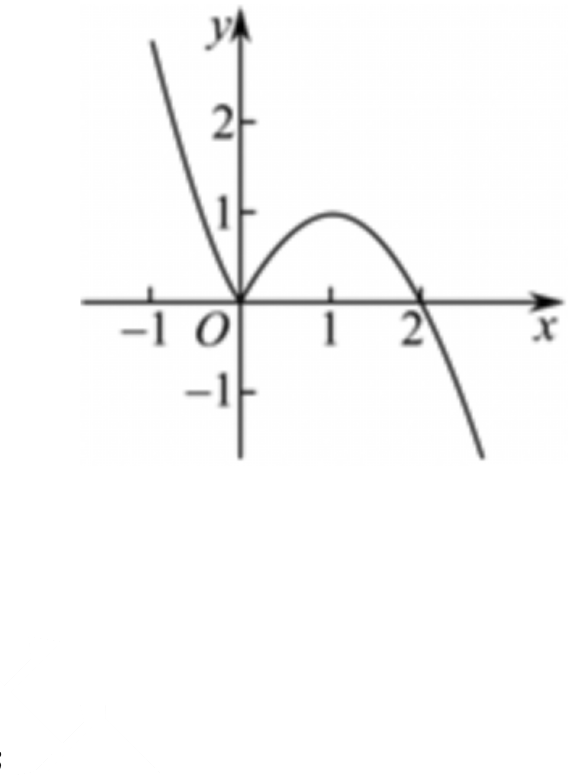
\includegraphics[width=0.20\textwidth]{figures/gao83_q15_graph.png}
\end{center}
\step{由 $[f(x)]^2+af(x)<0$ 得 $[f(x)+a]f(x)<0$，}
\step{当 $a=0$ 时，$[f(x)]^2<0$，不等式无解；}
\step{当 $a>0$ 时，由 $[f(x)+a]f(x)<0$ 得 $-a<f(x)<0$，}
\step{若不等式恰有 $1$ 个整数解，则整数解为 $3$，}
\step{又 $f(3)=-3$，$f(4)=-8$，所以 $-8\leqslant-a<-3$，所以 $3<a\leqslant8$；}
\step{当 $a<0$ 时，由 $[f(x)+a]f(x)<0$ 得 $0<f(x)<-a$，此时有多个解，故舍去；}
\step{综上所述，实数 $a$ 的取值范围为 $(3,8]$. 故选 $C$.}
\solend
\fi

\item 设函数 $f(x)=\begin{cases}\lvert2^x-1\rvert,&x\leqslant2\\ -x+7,&x>2\end{cases}$，若互不相等的实数 $a$、$b$、$c$ 满足 $f(a)=f(b)=f(c)$，
则 $2^a+2^b+2^c$ 的取值范围是\mbox{（\quad）}

\keepwithprev
A. $(8,9)$\qquad B. $(65,129)$\qquad C. $(64,128)$\qquad D. $(66,130)$

\ifanswer
\solbegin
\step{作出函数 $f(x)=\begin{cases}\lvert2^x-1\rvert,&x\leqslant2\\ -x+7,&x>2\end{cases}$ 的图象如图，}
\begin{center}
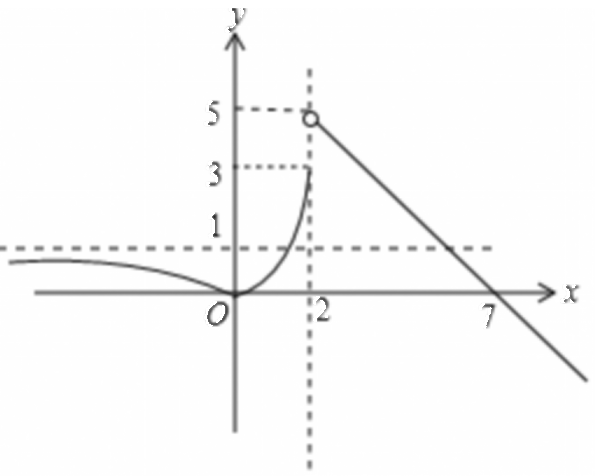
\includegraphics[width=0.22\textwidth]{figures/gao83_q16_graph.png}
\end{center}
\step{不妨设 $a<b<c$，由 $f(a)=f(b)$，得 $1-2^a=2^b-1$，则 $2^a+2^b=2$.}
\step{由 $f(-c)-c+6\in(0,1)$，得 $c\in(6,7)$，则 $64<2^c<128$，}
\step{所以 $66<2^a+2^b+2^c<130$，即 $2^a+2^b+2^c$ 的取值范围是 $(66,130)$. 故选 $D$.}
\solend
\fi

\end{enumerate}

\bigsec{三、解答题}

\begin{enumerate}
\setcounter{enumi}{16}

\item 已知幂函数 $f(x)$ 与一次函数 $g(x)$ 的图象都经过点 $(4,2)$，且 $f(9)=g(5)$.

（1）求 $f(x)$ 与 $g(x)$ 的解析式；

（2）求函数 $h(x)=g(x)-f(x)$ 在 $[0,4]$ 上的值域.

\ansspace*[8]

\ifanswer
\solbegin
\stepm{（1）}{设 $f(x)=x^\alpha$，$g(x)=kx+b$，则 $4^\alpha=2$，即 $\alpha=\dfrac12$，}
\step{$\begin{cases}4k+b=2\\ 3=5k+b\end{cases}$，则 $k=1$，$b=-2$，所以 $f(x)=\sqrt x$，$g(x)=x-2$；}
\stepm{（2）}{$h(x)=g(x)-f(x)=x-\sqrt x-2$，}
\step{令 $t=\sqrt x$，则 $t\in[0,2]$，原函数可化为 $p(t)=t^2-t-2$，}
\step{当 $t=\dfrac12$ 时，函数取得最小值 $-\dfrac94$，当 $t=2$ 时，函数取得最大值 $0$，}
\step{即函数值域为 $\left[-\dfrac94,0\right]$.}
\solend
\fi

\item 目前某县有 $100$ 万人. 经过 $x$ 年后为 $y$ 万人. 如果年平均增长率是 $1.2\%$. 请回答下列问题：

（1）写出 $y$ 关于 $x$ 的函数解析式.

（2）计算 $10$ 年后该县的人口总数（精确到 $0.1$ 万人）.

（3）计算大约多少年后该县的人口总数将达到 $120$ 万（精确到 $1$ 年）.

\ansspace*[9]

\ifanswer
\solbegin
\stepm{（1）}{当 $x=1$ 时，$y=100+100\times1.2\%=100(1+1.2\%)$，}
\step{当 $x=2$ 时，$y=100(1+1.2\%)+100(1+1.2\%)\times1.2\%=100(1+1.2\%)^2$，}
\step{当 $x=3$ 时，$y=100(1+1.2\%)^2+100(1+1.2\%)^2\times1.2\%=100(1+1.2\%)^3$，}
\step{$\cdots\cdots$}
\step{故 $y$ 关于 $x$ 的函数解析式为 $y=100(1+1.2\%)^x\,(x\in\N^*)$；}
\stepm{（2）}{当 $x=10$ 时，$y=100(1+1.2\%)^{10}=100\times1.012^{10}\approx112.7$，}
\step{故 $10$ 年后该县的人口总数约为 $112.7$ 万人；}
\stepm{（3）}{设 $x$ 年后该县的人口总数将达到 $120$ 万，即 $y=100(1+1.2\%)^x=120$，}
\step{解得 $x=\log_{1.012}\dfrac{120}{100}\approx16$，故大约 $16$ 年后该县的人口总数将达到 $120$ 万.}
\solend
\fi

\item 已知 $a>0$ 且 $a\neq1$，$m>0$，函数 $f(x)=(m^2+m-5)a^x$ 是指数函数，且 $f(2)=4$.

（1）求实数 $m$ 和 $a$ 的值；

（2）$f(2x)-2f(x)+2\geqslant nf(x)$ 对任意 $x\in[-1,2]$ 恒成立，求实数 $n$ 的取值范围；

（3）若关于 $x$ 的方程 $f(2x)-(2k+8)f(x)+2k+7b=0$ 有两个不相等的实数根，且一根
大于 $0$，另一根小于 $0$，其中 $k>0$，求整数 $b$ 的最大值.

\ansspace*[11]

\ifanswer
\solbegin
\stepm{（1）}{因为函数 $f(x)=(m^2+m-5)a^x$ 是指数函数，}
\step{所以 $m^2+m-5=1$，即 $m^2+m-6=0$，解得 $m=2$ 或 $m=-3$，}
\step{又 $m>0$，所以 $m=2$，又 $f(2)=a^2=4$，$a>0$ 且 $a\neq1$，所以 $a=2$；}
\stepm{（2）}{由（1）得 $f(x)=2^x$，}
\step{由题意 $2^{2x}-2\cdot2^x+2\geqslant n2^x$ 对任意 $x\in[-1,2]$ 恒成立，}
\step{所以 $n\leqslant2^x-2+\dfrac2{2^x}$ 对任意 $x\in[-1,2]$ 恒成立，则 $n\leqslant\left(2^x-2+\dfrac2{2^x}\right)_{\min}$，}
\step{记 $g(x)=2^x-2+\dfrac2{2^x}$，$x\in[-1,2]$，}
\step{令 $t=2^x$，因为 $x\in[-1,2]$，所以 $t\in\left[\dfrac12,4\right]$，则 $y=t+\dfrac2t-2$，$t\in\left[\dfrac12,4\right]$，}
\step{函数 $y=t+\dfrac2t-2$ 在 $\left[\dfrac12,\sqrt2\right]$ 上严格减，在 $[\sqrt2,4]$ 上严格增，}
\step{所以 $y=t+\dfrac2t-2$ 的最小值为 $\sqrt2+\dfrac2{\sqrt2}-2=2\sqrt2-2$，}
\step{所以 $n\leqslant2\sqrt2-2$，即实数 $n$ 的取值范围为 $(-\infty,2\sqrt2-2]$；}
\stepm{（3）}{方程 $f(2x)-(2k+8)f(x)+2k+7b=0$，}
\step{即方程 $2^{2x}-(2k+8)2^x+2k+7b=0$，即方程 $(2^x)^2-(2k+8)2^x+2k+7b=0$，}
\step{令 $t=2^x>0$，则方程 $t^2-(2k+8)t+2k+7b=0$，}
\step{因为关于 $x$ 的方程 $f(2x)-(2k+8)f(x)+2k+7b=0$ 的一根大于 $0$，另一根小于 $0$，}
\step{所以关于 $t$ 的方程 $t^2-(2k+8)t+2k+7b=0$ 的一根大于 $1$，另一根大于 $0$ 且小于 $1$，}
\step{记 $h(t)=t^2-(2k+8)t+2k+7b$，}
\step{所以 $\begin{cases}h(1)=1^2-(2k+8)\cdot1+2k+7b<0\\ h(0)=2k+7b>0\\ k>0\end{cases}$，所以 $\begin{cases}b<1\\ b>-\dfrac27k\\ k>0\end{cases}$，}
\step{所以整数 $b$ 的最大值为 $0$.}
\solend
\fi

\item 已知幂函数 $f(x)=(p^2-3p+3)x^{p^2-\frac32p-\frac12}$ 满足 $f(2)<f(4)$.

（1）求函数 $f(x)$ 的解析式；

（2）若函数 $g(x)=f^2(x)+mf(x)$，$x\in[1,9]$，是否存在实数 $m$ 使得 $g(x)$ 的最小值为 $0$？
若存在，求出 $m$ 的值；若不存在，说明理由.

（3）若函数 $h(x)=n-f(x+3)$，是否存在实数 $a$、$b\,(a<b)$，使函数 $h(x)$ 在 $[a,b]$ 上的
值域为 $[a,b]$？若存在，求出实数 $n$ 的取值范围；若不存在，说明理由.

\ansspace*[12]

\ifanswer
\solbegin
\stepm{（1）}{因为 $f(x)$ 是幂函数，所以 $p^2-3p+3=1$，解得 $p=1$ 或 $p=2$，}
\step{当 $p=1$ 时，$f(x)=\dfrac1x$，不满足 $f(2)<f(4)$.}
\step{当 $p=2$ 时，$f(x)=\sqrt x$，满足 $f(2)<f(4)$.}
\step{故 $p=2$，函数 $f(x)$ 的解析式为 $f(x)=\sqrt x$；}
\stepm{（2）}{由函数 $g(x)=f^2(x)+mf(x)$，即 $g(x)=(\sqrt x)^2+m\sqrt x$，}
\step{令 $t=\sqrt x$，因为 $x\in[1,9]$，所以 $t\in[1,3]$，}
\step{记 $k(x)=t^2+mt$，其对称轴 $t=-\dfrac m2$，}
\step{①当 $-\dfrac m2\leqslant1$，即 $m\geqslant-2$ 时，则 $k(x)_{\min}=k(1)=1+m=0$，解得 $m=-1$；}
\step{②当 $1<-\dfrac m2<3$ 时，即 $-6<m<-2$，则 $k(x)_{\min}=k\left(-\dfrac m2\right)=-\dfrac{m^2}4=0$，}
\step{解得 $m=0$，不满足，舍去；}
\step{③当 $-\dfrac m2\geqslant3$ 时，即 $m\leqslant-6$ 时，则 $k(x)_{\min}=k(3)=3m+9=0$，解得 $m=-3$，}
\step{不满足，舍去；}
\step{综上所述，存在 $m=-1$ 使得 $g(x)$ 的最小值为 $0$；}
\stepm{（3）}{由函数 $h(x)=n-f(x+3)=n-\sqrt{x+3}$ 在定义域内为严格减函数，}
\step{若存在实数 $a$、$b\,(a<b)$，使函数 $h(x)$ 在 $[a,b]$ 上的值域为 $[a,b]$，}
\step{则 $h(x)=\begin{cases}n-\sqrt{a+3}=b\text{ ①}\\ n-\sqrt{b+3}=a\text{ ②}\end{cases}$，}
\step{两式相减得 $\sqrt{a+3}-\sqrt{b+3}=a-b=(a+3)-(b+3)$，}
\step{所以 $\sqrt{a+3}+\sqrt{b+3}=1$ ③，}
\step{将③代入②得 $n=a+\sqrt{b+3}=a+1-\sqrt{a+3}$，}
\step{令 $t=\sqrt{a+3}$，因为 $a<b$，所以 $0\leqslant t<\dfrac12$，得 $n=t^2-t-2=\left(t-\dfrac12\right)^2-\dfrac94$，}
\step{故实数 $n$ 的取值范围为 $\left(-\dfrac94,-2\right]$.}
\solend
\fi

\item 定理（三角不等式），对于任意的 $a$、$b\in\R$，恒有 $\bigl\lvert\lvert a\rvert-\lvert b\rvert\bigr\rvert\leqslant\lvert a\pm b\rvert\leqslant\lvert a\rvert+\lvert b\rvert$. 定义：
已知 $n\in\N$ 且 $n\geqslant3$，对于有序数组 $a_1$、$a_2$、$\cdots$、$a_n$，称 $\lvert a_1-a_2\rvert+\lvert a_2-a_3\rvert+\cdots+\lvert a_{n-1}-a_n\rvert$
为有序数组 $a_1$、$a_2$、$\cdots$、$a_n$ 的波动距离，记作 $f(a_1,a_2,\cdots,a_n)$，即
$f(a_1,a_2,\cdots,a_n)=\lvert a_1-a_2\rvert+\lvert a_2-a_3\rvert+\cdots+\lvert a_{n-1}-a_n\rvert$，请根据上述信息解决以下几个问题：

（1）求函数 $y=\lvert x-2\rvert+\lvert x-4\rvert$ 的最小值，并指出函数取到最小值时 $x$ 的取值范围；

（2）①求有序数组 $2$、$5$、$3$、$4$ 的波动距离 $f(2,5,3,4)$；

②求证：若 $a$、$b$、$c$、$d\in\R$ 且 $a<b<c$，则 $f(a,b,c,d)\leqslant f(a,c,b,d)$；

（3）同理可证得命题“若 $a$、$b$、$c$、$d\in\R$ 且 $c<b<a$ 时，$f(a,b,c,d)\leqslant f(a,c,b,d)$”也
是真命题（注：该命题无需证明，需要时可直接使用）.

设两两不相等的四个实数 $a_1$、$a_2$、$a_3$、$a_4\in\{3^1,3^2,3^3,3^4\}$，求有序数组 $a_1$、$a_2$、$a_3$、$a_4$ 的
波动距离 $f(a_1,a_2,a_3,a_4)$ 的最大值.

\ansspace*[14]

\ifanswer
\solbegin
\stepm{（1）}{由三角不等式得 $\bigl\lvert\lvert a\rvert-\lvert b\rvert\bigr\rvert\leqslant\lvert a\pm b\rvert\leqslant\lvert a\rvert+\lvert b\rvert$，}
\step{当且仅当 $\lvert a+b\rvert^2=(\lvert a\rvert+\lvert b\rvert)^2$ 时，}
\step{即当 $-ab=\lvert ab\rvert$ 时，即当 $ab\leqslant0$ 时取等号，}
\step{由三角不等式得 $y=\lvert x-2\rvert+\lvert x-4\rvert\geqslant\lvert(x-2)-(x-4)\rvert=2$，}
\step{当且仅当 $(x-2)(x-4)\leqslant0$ 时，即 $2\leqslant x\leqslant4$ 时取等号，}
\step{因此，函数 $y=\lvert x-2\rvert+\lvert x-4\rvert$ 的最小值为 $2$，此时 $x$ 的取值范围是 $[2,4]$.}
\stepm{（2）}{①由题中定义得 $f(2,5,3,4)=\lvert2-5\rvert+\lvert5-3\rvert+\lvert3-4\rvert=6$；}
\step{②$f(a,b,c,d)-f(a,c,b,d)=\lvert a-b\rvert+\lvert c-d\rvert-\lvert a-c\rvert-\lvert b-d\rvert$，}
\step{因为 $a<b<c$，所以 $\lvert a-b\rvert-\lvert a-c\rvert=-\lvert b-c\rvert$，$\lvert c-d\rvert-\lvert b-d\rvert\leqslant\lvert b-c\rvert$，}
\step{所以 $f(a,b,c,d)-f(a,c,b,d)\leqslant0$，即 $f(a,b,c,d)\leqslant f(a,c,b,d)$，}
\stepm{（3）}{$f(a,b,c,d)=\lvert a-b\rvert+\lvert b-c\rvert+\lvert c-d\rvert$}
\step{$=\lvert d-c\rvert+\lvert c-b\rvert+\lvert b-a\rvert=f(d,c,b,a)$，}
\step{当 $f(a_1,a_2,a_3,a_4)$ 取得最大值时，$a_2=\max\{a_1,a_2,a_3\}$ 或 $a_2=\min\{a_1,a_2,a_3\}$，}
\step{同理 $a_3=\max\{a_2,a_3,a_4\}$ 或 $a_3=\min\{a_2,a_3,a_4\}$，}
\step{若 $a_2=\max\{a_1,a_2,a_3\}$，则 $a_2>a_3$，所以 $a_3=\min\{a_2,a_3,a_4\}$，}
\step{故 $f(a_1,a_2,a_3,a_4)=\lvert a_1-a_2\rvert+\lvert a_2-a_3\rvert+\lvert a_3-a_4\rvert=a_2-a_1+a_2-a_3+a_4-a_3$}
\step{$=2a_2+a_4-2a_3-a_1\leqslant2\times3^4+3^3-2\times3^1-3^2=174$，}
\step{当且仅当 $a_1=3^2$，$a_2=3^4$，$a_3=3^1$，$a_4=3^3$ 时取等号，}
\step{所以 $f(3^2,3^4,3^1,3^3)$ 为 $f(a_1,a_2,a_3,a_4)$ 的最大值，}
\step{若 $a_2=\min\{a_1,a_2,a_3\}$，则 $a_2<a_3$，所以 $a_3=\max\{a_2,a_3,a_4\}$，}
\step{同理可得 $f(3^3,3^4,3^1,3^2)$ 为 $f(a_1,a_2,a_3,a_4)$ 的最大值，}
\step{综上所述，$f(a_1,a_2,a_3,a_4)$ 的最大值为 $174$.}
\solend
\fi

\end{enumerate}

\end{document}
"
% 紧凑版：xelatex "\def\iscompact{1}% 高一83_交附闵行_周末作业10.23.tex
%   —— 高一上数学“2026-2027 年交附闵行高一上周末作业 10.23”（讲评版）
% 试卷版：xelatex 高一83_交附闵行_周末作业10.23.tex
% 答案版：xelatex "\def\isanswer{1}\input{高一83_交附闵行_周末作业10.23.tex}"
% 紧凑版：xelatex "\def\iscompact{1}\input{高一83_交附闵行_周末作业10.23.tex}"
%
% 原始材料：微信公众号“魔都数学加油站”文章，连载“27学年高一83”；
% 原文标题“27学年高一83——2026-2027年上海市交附闵行高一上周末作业10.23”；
% 原文链接：https://mp.weixin.qq.com/s/t5AfTwQXg4Sj4i_Dl5rgXA。
% 页面标注发布时间 2026-10-26 20:15（上海）。
% 正文为 12 张 PNG 页（`原图/高一83_交附闵行_周末作业10.23/01..12.png`），
% 尺寸混排（第 1—8 页为 4762×6735，第 9—12 页为 2560×3620），均按页序读取。
%
% 篇幅与题号：原卷自第 3 题起编号（第 1、2 题不在原文内）。填空题 3—12（10 题）、
% 选择题 13—16（4 题）、解答题 17—21（5 题），共 19 题。
%
% 讲评版：19 题全部印【解析】，本稿不另提 \ans{}；选择题答案在解析末句“故选 C／B／C／D”。
%
% 副标题：原卷未印副标题。本稿按内容标作“函数与导数”（本卷考幂函数、指数函数、
% 对数与函数应用，属“函数与导数”模块；副标题只用知识模块名，见 README 说明）。
%
% 与原卷的排版差异：
%   ① 原卷每题下直接印【解析】，本稿按全稿惯例将解析置于答案版；
%   ② 原卷未印副标题，本稿补出；填空横线统一排 \blankline[4.4em]；
%   ③ 原卷数集记号排斜体 $R$、$Z$、$N$，本稿按全稿惯例改用 $\R$、$\Z$、$\N$；
%   ④ 第 17—21 题的子问用行内“（1）（2）（3）”段，解析中的子问标号用 \stepm；
%   ⑤ 解答题按惯例加 \ansspace；选择题括号排 \mbox{（\quad）}；
%   ⑥ 第 15、16 题解析各有一幅函数图象，裁自原图（第 6 页）后去粉色水印、转灰度，
%      仅答案版出。
%
% 行数核对：逐题数 \step/\stepm 条数，合计 145 条（Q3：1；Q4：1；Q5：4；Q6：5；
% Q7：2；Q8：7；Q9：10；Q10：5；Q11：6；Q12：8；Q13：3；Q14：4；Q15：8；
% Q16：4；Q17：6；Q18：9；Q19：19；Q20：21；Q21：22）。原卷解析的换行
% 按语意合并，未逐行强拆。
%
\documentclass[a4paper,11pt]{article}
\usepackage{common}

\begin{document}

\examtitlest[4]{2026--2027 年交附闵行高一上周末作业 10.23}{函数与导数}

\bigsec{一、填空题}

\begin{enumerate}
\setcounter{enumi}{2}

\item 已知 $10^a=2$，$10^b=5$，则 $10^{3a-2b}$ 的值为\blankline[4.4em].

\ifanswer
\solbegin
\step{$10^{3a-2b}=\dfrac{10^{3a}}{10^{2b}}=\dfrac{(10^a)^3}{(10^b)^2}=\dfrac{2^3}{5^2}=\dfrac8{25}$.}
\solend
\fi

\item 根式 $a\sqrt{-a}$ 化成分数指数幂是\blankline[4.4em].

\ifanswer
\solbegin
\step{$a\sqrt{-a}=a(-a)^{\frac12}=-(-a)(-a)^{\frac12}=-(-a)^{\frac32}$.}
\solend
\fi

\item 已知数列 $\{a_n\}$ 的通项公式为 $a_n=\left(\dfrac49\right)^{n-1}-\left(\dfrac23\right)^{n-1}$，在下列说法中：①有最大项；
②有最小项；③没有最大项；④没有最小项. 正确的是\blankline[3.6em]（填序号）.

\ifanswer
\solbegin
\step{令 $t=\left(\dfrac23\right)^{n-1}$，则 $t\in\left\{1,\dfrac23,\dfrac49,\dfrac8{27},\cdots\right\}\subset(0,1]$，$t$ 是关于 $n$ 的减函数，}
\step{则 $a_n=t^2-t=\left(t-\dfrac12\right)^2-\dfrac14$，}
\step{所以当 $t=1$ 即 $n=1$ 时 $a_n$ 取得最大为 $0$，当 $t=\dfrac49$ 即 $n=3$ 时 $a_n$ 取得最小为 $-\dfrac{20}{81}$，}
\step{所以 $a_n$ 既有最大项又有最小项，故①和②正确.}
\solend
\fi

\item 已知 $f(x)=\mathrm{e}^{x-\frac12}-\mathrm{e}^{-x+\frac12}+\dfrac{4x}{2x-1}$，则
$f\left(\dfrac1{2020}\right)+f\left(\dfrac2{2020}\right)+f\left(\dfrac3{2020}\right)+\cdots+f\left(\dfrac{1009}{2020}\right)+f\left(\dfrac{1011}{2020}\right)+\cdots+f\left(\dfrac{2019}{2020}\right)$ 的
值为\blankline[4.4em].

\ifanswer
\solbegin
\step{因为 $f(x)+f(1-x)=\mathrm{e}^{x-\frac12}-\mathrm{e}^{-x+\frac12}+\dfrac{4x}{2x-1}+\mathrm{e}^{(1-x)-\frac12}-\mathrm{e}^{-(1-x)+\frac12}+\dfrac{4(1-x)}{2(1-x)-1}$}
\step{$=\dfrac{4x}{2x-1}+\dfrac{4-4x}{1-2x}=\dfrac{4(2x-1)}{2x-1}=4$，}
\step{记 $S=f\left(\dfrac1{2020}\right)+f\left(\dfrac2{2020}\right)+\cdots+f\left(\dfrac{2019}{2020}\right)$，}
\step{又 $S=f\left(\dfrac{2019}{2020}\right)+f\left(\dfrac{2018}{2020}\right)+\cdots+f\left(\dfrac2{2020}\right)+f\left(\dfrac1{2020}\right)$，}
\step{对齐相加得 $2S=2018\times4$，所以 $S=4036$.}
\solend
\fi

\item 不等式 $2^{x^2-2x-3}<\left(\dfrac12\right)^{3(x-1)}$ 的解集为\blankline[4.4em].

\ifanswer
\solbegin
\step{由 $2^{x^2-2x-3}<\left(\dfrac12\right)^{3(x-1)}$ 得 $x^2-2x-3<-3(x-1)$，即 $x^2+x-6<0$，}
\step{故解集为 $(-3,2)$.}
\solend
\fi

\item 函数 $f(x)=x^{\ln5}+x^{\ln12}-13^{\ln x}$ 的零点是\blankline[4.4em]. 附：$a^{\log_bc}=c^{\log_ba}$
（$a>0$，$b>0$，$c>0$，$b\neq1$）.

\ifanswer
\solbegin
\step{函数 $f(x)=x^{\ln5}+x^{\ln12}-13^{\ln x}$，}
\step{若 $f(x)=x^{\ln5}+x^{\ln12}-13^{\ln x}=0$，变形得 $x^{\ln5}+x^{\ln12}=13^{\ln x}$，}
\step{又 $a^{\log_bc}=c^{\log_ba}$（$a>0$，$b>0$，$c>0$，$b\neq1$），得 $5^{\ln x}+12^{\ln x}=13^{\ln x}$，}
\step{令 $g(t)=\left(\dfrac5{13}\right)^t+\left(\dfrac{12}{13}\right)^t-1$，易得 $g(t)$ 严格减，所以 $g(t)=0$ 至多有一解，}
\step{即 $\left(\dfrac5{13}\right)^t+\left(\dfrac{12}{13}\right)^t-1=0$ 至多有一解，变形得方程 $5^t+12^t=13^t$ 至多有一解，}
\step{易得 $t=2$ 时，有 $5^2+12^2=13^2$ 成立，则方程 $5^t+12^t=13^t$ 有唯一解 $t=2$，}
\step{即 $\ln x=2$，解得 $x=\mathrm{e}^2$，即函数 $f(x)$ 的零点为 $\mathrm{e}^2$.}
\solend
\fi

\item 已知幂函数 $f(x)=(m^2-2m-2)x^{m^2+m-2}$ 在 $(0,+\infty)$ 上是严格减函数，则不等式
$f(x-1)<f(3-2x)$ 的解集为\blankline[4.4em].

\ifanswer
\solbegin
\step{因为 $f(x)$ 为幂函数，所以 $m^2-2m-2=1$，解得 $m=-1$ 或 $m=3$；}
\step{当 $m=3$ 时，$f(x)=x^{10}$ 在 $(0,+\infty)$ 上严格增，不合题意；}
\step{当 $m=-1$ 时，$f(x)=x^{-2}$ 在 $(0,+\infty)$ 上严格减，符合题意；}
\step{综上所述，$m=-1$；}
\step{因为 $f(x)=x^{-2}$ 的定义域为 $(-\infty,0)\cup(0,+\infty)$，$f(-x)=(-x)^{-2}=x^{-2}=f(x)$，}
\step{所以 $f(x)$ 为定义在 $(-\infty,0)\cup(0,+\infty)$ 上的偶函数，}
\step{故 $f(x-1)=f(\lvert x-1\rvert)$，$f(3-2x)=f(\lvert3-2x\rvert)$，}
\step{$f(x-1)<f(3-2x)\Rightarrow f(\lvert x-1\rvert)<f(\lvert3-2x\rvert)\Rightarrow\lvert x-1\rvert>\lvert3-2x\rvert$}
\step{且 $\lvert x-1\rvert\neq0$，$\lvert3-2x\rvert\neq0$，解得 $\dfrac43<x<\dfrac32$ 或 $\dfrac32<x<2$，}
\step{所以 $f(x-1)<f(3-2x)$ 的解集为 $\left(\dfrac43,\dfrac32\right)\cup\left(\dfrac32,2\right)$.}
\solend
\fi

\item 若实数 $x_1$、$x_2$ 满足 $\mathrm{e}^{x_1}+x_1-3=0$，$x_2\ln x_2+3x_2-1=0$，则 $\dfrac{x_1x_2+1}{x_2}$ 的值为\blankline[4.4em].

\ifanswer
\solbegin
\step{易得 $x_2>0$，则 $\ln x_2+3-\dfrac1{x_2}=0$，即 $\mathrm{e}^{-\ln x_2}+(-\ln x_2)-3=0$.}
\step{设 $f(x)=\mathrm{e}^x+x-3$，则函数 $f(x)$ 在 $(-\infty,+\infty)$ 上严格增.}
\step{由 $\mathrm{e}^{x_1}+x_1-3=0$，$\mathrm{e}^{-\ln x_2}+(-\ln x_2)-3=0$，得 $f(x_1)=0$，$f(-\ln x_2)=0$，}
\step{所以 $f(x_1)=f(-\ln x_2)$，得 $x_1=-\ln x_2$，即 $\ln x_2=-x_1$，所以 $x_2=\mathrm{e}^{-x_1}$，得 $\dfrac1{x_2}=\mathrm{e}^{x_1}$.}
\step{因为 $\mathrm{e}^{x_1}+x_1-3=0$，所以 $\mathrm{e}^{x_1}+x_1=3$，所以 $\dfrac{x_1x_2+1}{x_2}=x_1+\dfrac1{x_2}=\mathrm{e}^{x_1}+x_1=3$.}
\solend
\fi

\item 已知 $\alpha$、$\beta$ 是方程 $9^x-2m\cdot3^x+m^2-1=0$ 的两个根，若 $\alpha+\beta=1$，则 $\alpha\beta=\blankline[4.4em]$.

\ifanswer
\solbegin
\step{由题意得方程 $9^x-2m\cdot3^x+m^2-1=0$ 有两个根，}
\step{则方程 $t^2-2mt+m^2-1=0$ 有二正根，则 $\begin{cases}\Delta=4m^2-4(m^2-1)\geqslant0\\ 2m>0\\ m^2-1>0\end{cases}$，解得 $m>1$，}
\step{又 $\alpha$、$\beta$ 是方程 $9^x-2m\cdot3^x+m^2-1=0$ 的两个根，则 $3^\alpha\times3^\beta=m^2-1$，}
\step{又 $\alpha+\beta=1$，则 $m^2-1=3^{\alpha+\beta}=3$，解得 $m=2$ 或 $m=-2$（舍），}
\step{则 $3^\alpha+3^\beta=2m=4$，又 $\alpha=1-\beta$，则 $3^{1-\beta}+3^\beta=4$，解得 $\beta=0$ 或 $\beta=1$，}
\step{则 $\begin{cases}\alpha=1\\ \beta=0\end{cases}$ 或 $\begin{cases}\alpha=0\\ \beta=1\end{cases}$，则 $\alpha\beta=0$.}
\solend
\fi

\item 已知实数 $a,b,c\in(1,+\infty)$，满足 $a^{\log_ba}\cdot b^{\log_cb}\cdot c^{\log_ac}=100$，则 $abc$ 的最大值为\blankline[4.4em].

\ifanswer
\solbegin
\step{由换底公式得 $\log_ba=\dfrac{\ln a}{\ln b}$，$\log_cb=\dfrac{\ln b}{\ln c}$，$\log_ac=\dfrac{\ln c}{\ln a}$，}
\step{设 $X=\ln a$，$Y=\ln b$，$Z=\ln c$，得 $a=\mathrm{e}^X$，$b=\mathrm{e}^Y$，$c=\mathrm{e}^Z$，}
\step{代入得 $a^{\log_ba}\cdot b^{\log_cb}\cdot c^{\log_ac}=a^{\frac{\ln a}{\ln b}}\cdot b^{\frac{\ln b}{\ln c}}\cdot c^{\frac{\ln c}{\ln a}}=(\mathrm{e}^X)^{\frac XY}\cdot(\mathrm{e}^Y)^{\frac YZ}\cdot(\mathrm{e}^Z)^{\frac ZX}=100$，}
\step{即 $\mathrm{e}^{\frac{X^2}Y+\frac{Y^2}Z+\frac{Z^2}X}=100$，两边取对数得 $\dfrac{X^2}Y+\dfrac{Y^2}Z+\dfrac{Z^2}X=\ln100$.}
\step{由 $a,b,c\in(1,+\infty)$，得 $X>0$，$Y>0$，$Z>0$，}
\step{由柯西不等式，得 $\left(\dfrac{X^2}Y+\dfrac{Y^2}Z+\dfrac{Z^2}X\right)(X+Y+Z)\geqslant(X+Y+Z)^2$，}
\step{即 $X+Y+Z\leqslant\dfrac{X^2}Y+\dfrac{Y^2}Z+\dfrac{Z^2}X=\ln100$，当且仅当 $X=Y=Z$ 时取等号，}
\step{因此 $(X+Y+Z)_{\max}=\ln100$，所以 $(abc)_{\max}=\mathrm{e}^{(X+Y+Z)_{\max}}=\mathrm{e}^{\ln100}=100$.}
\solend
\fi

\end{enumerate}

\bigsec{二、选择题}

\begin{enumerate}
\setcounter{enumi}{12}

\item 已知集合 $A=\{x\mid x=2k,k\in\Z\}$，$B=\{x\mid x=4k+2,\,k\in\Z\}$，则 $A\cup B=\mbox{（\quad）}$

\keepwithprev
A. $B$\qquad B. $\R$\qquad C. $A$\qquad D. 以上都不是

\ifanswer
\solbegin
\step{$B=\{x\mid x=4k+2,k\in\Z\}=\{x\mid x=2(2k+1),k\in\Z\}$，它表示奇数的 $2$ 倍组成的集合，}
\step{$A=\{x\mid x=2k,k\in\Z\}$，即集合 $A$ 是整数的 $2$ 倍组成的集合，}
\step{则 $B\subseteq A$，则 $A\cup B=A$. 故选 $C$.}
\solend
\fi

\item 教室通风的目的是通过空气的流动，排出室内的污浊空气和致病微生物，降低室内二氧化碳和致病微生物的浓度，送进室外的新鲜空气. 按照国家标准，教室内空气中二氧化碳日平均最高容许浓度应小于等于 $0.1\%$. 经测定，刚下课时，空气中含有 $0.2\%$ 的二氧化碳，若开窗通风后教室内二氧化碳的浓度为 $y\%$，且 $y$ 随时间 $t$（单位：分钟）的变化规律可以用函数 $y=0.05+\lambda\mathrm{e}^{-\frac t{12}}\,(\lambda\in\R)$ 描述，则该教室内的二氧化碳浓度达到国家标准至少需要的时间为\mbox{（\quad）}

\keepwithprev
A. $10$ 分钟\qquad B. $14$ 分钟\qquad C. $15$ 分钟\qquad D. $20$ 分钟

\ifanswer
\solbegin
\step{由题意得，当 $t=0$ 时，$y=0.2$，即 $0.05+\lambda\mathrm{e}^0=0.2$，解得 $\lambda=0.15$，}
\step{所以 $y=0.05+0.15\mathrm{e}^{-\frac t{12}}$，由题意得 $0.05+0.15\mathrm{e}^{-\frac t{12}}\leqslant0.1$，即 $\mathrm{e}^{-\frac t{12}}\leqslant\dfrac13$，}
\step{两边取对数得 $-\dfrac t{12}\leqslant-\ln3$，所以 $t\geqslant12\ln3\approx13.2$，}
\step{所以该教室内的二氧化碳浓度达到国家标准至少需要的时间为 $14$ 分钟. 故选 $B$.}
\solend
\fi

\item 已知函数 $f(x)=\begin{cases}-x^2+2x,&x\geqslant0\\ x^2-2x,&x<0\end{cases}$，若关于 $x$ 的不等式 $[f(x)]^2+af(x)<0$ 恰有 $1$ 个整数
解，则实数 $a$ 的最大值为\mbox{（\quad）}

\keepwithprev
A. $-2$\qquad B. $3$\qquad C. $8$\qquad D. $9$

\ifanswer
\solbegin
\step{作出 $f(x)$ 的图象，如图所示：}
\begin{center}
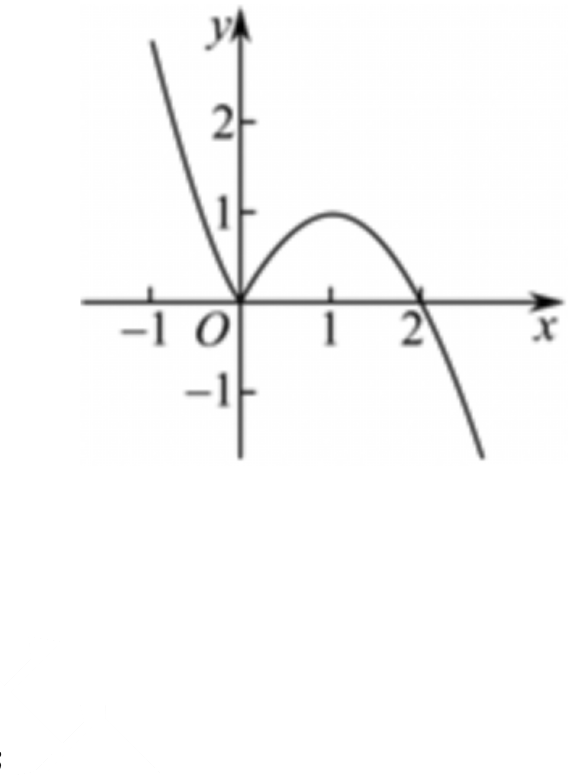
\includegraphics[width=0.20\textwidth]{figures/gao83_q15_graph.png}
\end{center}
\step{由 $[f(x)]^2+af(x)<0$ 得 $[f(x)+a]f(x)<0$，}
\step{当 $a=0$ 时，$[f(x)]^2<0$，不等式无解；}
\step{当 $a>0$ 时，由 $[f(x)+a]f(x)<0$ 得 $-a<f(x)<0$，}
\step{若不等式恰有 $1$ 个整数解，则整数解为 $3$，}
\step{又 $f(3)=-3$，$f(4)=-8$，所以 $-8\leqslant-a<-3$，所以 $3<a\leqslant8$；}
\step{当 $a<0$ 时，由 $[f(x)+a]f(x)<0$ 得 $0<f(x)<-a$，此时有多个解，故舍去；}
\step{综上所述，实数 $a$ 的取值范围为 $(3,8]$. 故选 $C$.}
\solend
\fi

\item 设函数 $f(x)=\begin{cases}\lvert2^x-1\rvert,&x\leqslant2\\ -x+7,&x>2\end{cases}$，若互不相等的实数 $a$、$b$、$c$ 满足 $f(a)=f(b)=f(c)$，
则 $2^a+2^b+2^c$ 的取值范围是\mbox{（\quad）}

\keepwithprev
A. $(8,9)$\qquad B. $(65,129)$\qquad C. $(64,128)$\qquad D. $(66,130)$

\ifanswer
\solbegin
\step{作出函数 $f(x)=\begin{cases}\lvert2^x-1\rvert,&x\leqslant2\\ -x+7,&x>2\end{cases}$ 的图象如图，}
\begin{center}
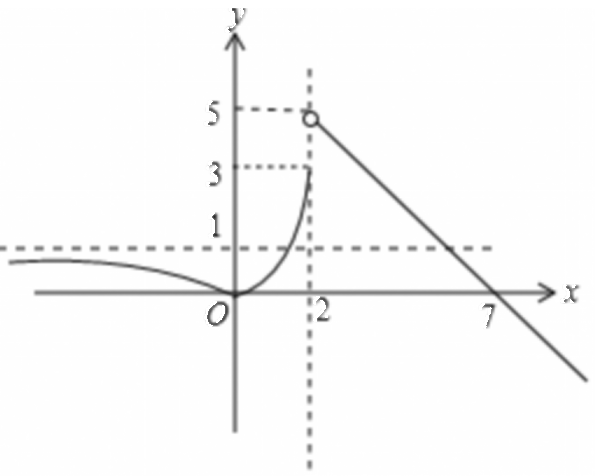
\includegraphics[width=0.22\textwidth]{figures/gao83_q16_graph.png}
\end{center}
\step{不妨设 $a<b<c$，由 $f(a)=f(b)$，得 $1-2^a=2^b-1$，则 $2^a+2^b=2$.}
\step{由 $f(-c)-c+6\in(0,1)$，得 $c\in(6,7)$，则 $64<2^c<128$，}
\step{所以 $66<2^a+2^b+2^c<130$，即 $2^a+2^b+2^c$ 的取值范围是 $(66,130)$. 故选 $D$.}
\solend
\fi

\end{enumerate}

\bigsec{三、解答题}

\begin{enumerate}
\setcounter{enumi}{16}

\item 已知幂函数 $f(x)$ 与一次函数 $g(x)$ 的图象都经过点 $(4,2)$，且 $f(9)=g(5)$.

（1）求 $f(x)$ 与 $g(x)$ 的解析式；

（2）求函数 $h(x)=g(x)-f(x)$ 在 $[0,4]$ 上的值域.

\ansspace*[8]

\ifanswer
\solbegin
\stepm{（1）}{设 $f(x)=x^\alpha$，$g(x)=kx+b$，则 $4^\alpha=2$，即 $\alpha=\dfrac12$，}
\step{$\begin{cases}4k+b=2\\ 3=5k+b\end{cases}$，则 $k=1$，$b=-2$，所以 $f(x)=\sqrt x$，$g(x)=x-2$；}
\stepm{（2）}{$h(x)=g(x)-f(x)=x-\sqrt x-2$，}
\step{令 $t=\sqrt x$，则 $t\in[0,2]$，原函数可化为 $p(t)=t^2-t-2$，}
\step{当 $t=\dfrac12$ 时，函数取得最小值 $-\dfrac94$，当 $t=2$ 时，函数取得最大值 $0$，}
\step{即函数值域为 $\left[-\dfrac94,0\right]$.}
\solend
\fi

\item 目前某县有 $100$ 万人. 经过 $x$ 年后为 $y$ 万人. 如果年平均增长率是 $1.2\%$. 请回答下列问题：

（1）写出 $y$ 关于 $x$ 的函数解析式.

（2）计算 $10$ 年后该县的人口总数（精确到 $0.1$ 万人）.

（3）计算大约多少年后该县的人口总数将达到 $120$ 万（精确到 $1$ 年）.

\ansspace*[9]

\ifanswer
\solbegin
\stepm{（1）}{当 $x=1$ 时，$y=100+100\times1.2\%=100(1+1.2\%)$，}
\step{当 $x=2$ 时，$y=100(1+1.2\%)+100(1+1.2\%)\times1.2\%=100(1+1.2\%)^2$，}
\step{当 $x=3$ 时，$y=100(1+1.2\%)^2+100(1+1.2\%)^2\times1.2\%=100(1+1.2\%)^3$，}
\step{$\cdots\cdots$}
\step{故 $y$ 关于 $x$ 的函数解析式为 $y=100(1+1.2\%)^x\,(x\in\N^*)$；}
\stepm{（2）}{当 $x=10$ 时，$y=100(1+1.2\%)^{10}=100\times1.012^{10}\approx112.7$，}
\step{故 $10$ 年后该县的人口总数约为 $112.7$ 万人；}
\stepm{（3）}{设 $x$ 年后该县的人口总数将达到 $120$ 万，即 $y=100(1+1.2\%)^x=120$，}
\step{解得 $x=\log_{1.012}\dfrac{120}{100}\approx16$，故大约 $16$ 年后该县的人口总数将达到 $120$ 万.}
\solend
\fi

\item 已知 $a>0$ 且 $a\neq1$，$m>0$，函数 $f(x)=(m^2+m-5)a^x$ 是指数函数，且 $f(2)=4$.

（1）求实数 $m$ 和 $a$ 的值；

（2）$f(2x)-2f(x)+2\geqslant nf(x)$ 对任意 $x\in[-1,2]$ 恒成立，求实数 $n$ 的取值范围；

（3）若关于 $x$ 的方程 $f(2x)-(2k+8)f(x)+2k+7b=0$ 有两个不相等的实数根，且一根
大于 $0$，另一根小于 $0$，其中 $k>0$，求整数 $b$ 的最大值.

\ansspace*[11]

\ifanswer
\solbegin
\stepm{（1）}{因为函数 $f(x)=(m^2+m-5)a^x$ 是指数函数，}
\step{所以 $m^2+m-5=1$，即 $m^2+m-6=0$，解得 $m=2$ 或 $m=-3$，}
\step{又 $m>0$，所以 $m=2$，又 $f(2)=a^2=4$，$a>0$ 且 $a\neq1$，所以 $a=2$；}
\stepm{（2）}{由（1）得 $f(x)=2^x$，}
\step{由题意 $2^{2x}-2\cdot2^x+2\geqslant n2^x$ 对任意 $x\in[-1,2]$ 恒成立，}
\step{所以 $n\leqslant2^x-2+\dfrac2{2^x}$ 对任意 $x\in[-1,2]$ 恒成立，则 $n\leqslant\left(2^x-2+\dfrac2{2^x}\right)_{\min}$，}
\step{记 $g(x)=2^x-2+\dfrac2{2^x}$，$x\in[-1,2]$，}
\step{令 $t=2^x$，因为 $x\in[-1,2]$，所以 $t\in\left[\dfrac12,4\right]$，则 $y=t+\dfrac2t-2$，$t\in\left[\dfrac12,4\right]$，}
\step{函数 $y=t+\dfrac2t-2$ 在 $\left[\dfrac12,\sqrt2\right]$ 上严格减，在 $[\sqrt2,4]$ 上严格增，}
\step{所以 $y=t+\dfrac2t-2$ 的最小值为 $\sqrt2+\dfrac2{\sqrt2}-2=2\sqrt2-2$，}
\step{所以 $n\leqslant2\sqrt2-2$，即实数 $n$ 的取值范围为 $(-\infty,2\sqrt2-2]$；}
\stepm{（3）}{方程 $f(2x)-(2k+8)f(x)+2k+7b=0$，}
\step{即方程 $2^{2x}-(2k+8)2^x+2k+7b=0$，即方程 $(2^x)^2-(2k+8)2^x+2k+7b=0$，}
\step{令 $t=2^x>0$，则方程 $t^2-(2k+8)t+2k+7b=0$，}
\step{因为关于 $x$ 的方程 $f(2x)-(2k+8)f(x)+2k+7b=0$ 的一根大于 $0$，另一根小于 $0$，}
\step{所以关于 $t$ 的方程 $t^2-(2k+8)t+2k+7b=0$ 的一根大于 $1$，另一根大于 $0$ 且小于 $1$，}
\step{记 $h(t)=t^2-(2k+8)t+2k+7b$，}
\step{所以 $\begin{cases}h(1)=1^2-(2k+8)\cdot1+2k+7b<0\\ h(0)=2k+7b>0\\ k>0\end{cases}$，所以 $\begin{cases}b<1\\ b>-\dfrac27k\\ k>0\end{cases}$，}
\step{所以整数 $b$ 的最大值为 $0$.}
\solend
\fi

\item 已知幂函数 $f(x)=(p^2-3p+3)x^{p^2-\frac32p-\frac12}$ 满足 $f(2)<f(4)$.

（1）求函数 $f(x)$ 的解析式；

（2）若函数 $g(x)=f^2(x)+mf(x)$，$x\in[1,9]$，是否存在实数 $m$ 使得 $g(x)$ 的最小值为 $0$？
若存在，求出 $m$ 的值；若不存在，说明理由.

（3）若函数 $h(x)=n-f(x+3)$，是否存在实数 $a$、$b\,(a<b)$，使函数 $h(x)$ 在 $[a,b]$ 上的
值域为 $[a,b]$？若存在，求出实数 $n$ 的取值范围；若不存在，说明理由.

\ansspace*[12]

\ifanswer
\solbegin
\stepm{（1）}{因为 $f(x)$ 是幂函数，所以 $p^2-3p+3=1$，解得 $p=1$ 或 $p=2$，}
\step{当 $p=1$ 时，$f(x)=\dfrac1x$，不满足 $f(2)<f(4)$.}
\step{当 $p=2$ 时，$f(x)=\sqrt x$，满足 $f(2)<f(4)$.}
\step{故 $p=2$，函数 $f(x)$ 的解析式为 $f(x)=\sqrt x$；}
\stepm{（2）}{由函数 $g(x)=f^2(x)+mf(x)$，即 $g(x)=(\sqrt x)^2+m\sqrt x$，}
\step{令 $t=\sqrt x$，因为 $x\in[1,9]$，所以 $t\in[1,3]$，}
\step{记 $k(x)=t^2+mt$，其对称轴 $t=-\dfrac m2$，}
\step{①当 $-\dfrac m2\leqslant1$，即 $m\geqslant-2$ 时，则 $k(x)_{\min}=k(1)=1+m=0$，解得 $m=-1$；}
\step{②当 $1<-\dfrac m2<3$ 时，即 $-6<m<-2$，则 $k(x)_{\min}=k\left(-\dfrac m2\right)=-\dfrac{m^2}4=0$，}
\step{解得 $m=0$，不满足，舍去；}
\step{③当 $-\dfrac m2\geqslant3$ 时，即 $m\leqslant-6$ 时，则 $k(x)_{\min}=k(3)=3m+9=0$，解得 $m=-3$，}
\step{不满足，舍去；}
\step{综上所述，存在 $m=-1$ 使得 $g(x)$ 的最小值为 $0$；}
\stepm{（3）}{由函数 $h(x)=n-f(x+3)=n-\sqrt{x+3}$ 在定义域内为严格减函数，}
\step{若存在实数 $a$、$b\,(a<b)$，使函数 $h(x)$ 在 $[a,b]$ 上的值域为 $[a,b]$，}
\step{则 $h(x)=\begin{cases}n-\sqrt{a+3}=b\text{ ①}\\ n-\sqrt{b+3}=a\text{ ②}\end{cases}$，}
\step{两式相减得 $\sqrt{a+3}-\sqrt{b+3}=a-b=(a+3)-(b+3)$，}
\step{所以 $\sqrt{a+3}+\sqrt{b+3}=1$ ③，}
\step{将③代入②得 $n=a+\sqrt{b+3}=a+1-\sqrt{a+3}$，}
\step{令 $t=\sqrt{a+3}$，因为 $a<b$，所以 $0\leqslant t<\dfrac12$，得 $n=t^2-t-2=\left(t-\dfrac12\right)^2-\dfrac94$，}
\step{故实数 $n$ 的取值范围为 $\left(-\dfrac94,-2\right]$.}
\solend
\fi

\item 定理（三角不等式），对于任意的 $a$、$b\in\R$，恒有 $\bigl\lvert\lvert a\rvert-\lvert b\rvert\bigr\rvert\leqslant\lvert a\pm b\rvert\leqslant\lvert a\rvert+\lvert b\rvert$. 定义：
已知 $n\in\N$ 且 $n\geqslant3$，对于有序数组 $a_1$、$a_2$、$\cdots$、$a_n$，称 $\lvert a_1-a_2\rvert+\lvert a_2-a_3\rvert+\cdots+\lvert a_{n-1}-a_n\rvert$
为有序数组 $a_1$、$a_2$、$\cdots$、$a_n$ 的波动距离，记作 $f(a_1,a_2,\cdots,a_n)$，即
$f(a_1,a_2,\cdots,a_n)=\lvert a_1-a_2\rvert+\lvert a_2-a_3\rvert+\cdots+\lvert a_{n-1}-a_n\rvert$，请根据上述信息解决以下几个问题：

（1）求函数 $y=\lvert x-2\rvert+\lvert x-4\rvert$ 的最小值，并指出函数取到最小值时 $x$ 的取值范围；

（2）①求有序数组 $2$、$5$、$3$、$4$ 的波动距离 $f(2,5,3,4)$；

②求证：若 $a$、$b$、$c$、$d\in\R$ 且 $a<b<c$，则 $f(a,b,c,d)\leqslant f(a,c,b,d)$；

（3）同理可证得命题“若 $a$、$b$、$c$、$d\in\R$ 且 $c<b<a$ 时，$f(a,b,c,d)\leqslant f(a,c,b,d)$”也
是真命题（注：该命题无需证明，需要时可直接使用）.

设两两不相等的四个实数 $a_1$、$a_2$、$a_3$、$a_4\in\{3^1,3^2,3^3,3^4\}$，求有序数组 $a_1$、$a_2$、$a_3$、$a_4$ 的
波动距离 $f(a_1,a_2,a_3,a_4)$ 的最大值.

\ansspace*[14]

\ifanswer
\solbegin
\stepm{（1）}{由三角不等式得 $\bigl\lvert\lvert a\rvert-\lvert b\rvert\bigr\rvert\leqslant\lvert a\pm b\rvert\leqslant\lvert a\rvert+\lvert b\rvert$，}
\step{当且仅当 $\lvert a+b\rvert^2=(\lvert a\rvert+\lvert b\rvert)^2$ 时，}
\step{即当 $-ab=\lvert ab\rvert$ 时，即当 $ab\leqslant0$ 时取等号，}
\step{由三角不等式得 $y=\lvert x-2\rvert+\lvert x-4\rvert\geqslant\lvert(x-2)-(x-4)\rvert=2$，}
\step{当且仅当 $(x-2)(x-4)\leqslant0$ 时，即 $2\leqslant x\leqslant4$ 时取等号，}
\step{因此，函数 $y=\lvert x-2\rvert+\lvert x-4\rvert$ 的最小值为 $2$，此时 $x$ 的取值范围是 $[2,4]$.}
\stepm{（2）}{①由题中定义得 $f(2,5,3,4)=\lvert2-5\rvert+\lvert5-3\rvert+\lvert3-4\rvert=6$；}
\step{②$f(a,b,c,d)-f(a,c,b,d)=\lvert a-b\rvert+\lvert c-d\rvert-\lvert a-c\rvert-\lvert b-d\rvert$，}
\step{因为 $a<b<c$，所以 $\lvert a-b\rvert-\lvert a-c\rvert=-\lvert b-c\rvert$，$\lvert c-d\rvert-\lvert b-d\rvert\leqslant\lvert b-c\rvert$，}
\step{所以 $f(a,b,c,d)-f(a,c,b,d)\leqslant0$，即 $f(a,b,c,d)\leqslant f(a,c,b,d)$，}
\stepm{（3）}{$f(a,b,c,d)=\lvert a-b\rvert+\lvert b-c\rvert+\lvert c-d\rvert$}
\step{$=\lvert d-c\rvert+\lvert c-b\rvert+\lvert b-a\rvert=f(d,c,b,a)$，}
\step{当 $f(a_1,a_2,a_3,a_4)$ 取得最大值时，$a_2=\max\{a_1,a_2,a_3\}$ 或 $a_2=\min\{a_1,a_2,a_3\}$，}
\step{同理 $a_3=\max\{a_2,a_3,a_4\}$ 或 $a_3=\min\{a_2,a_3,a_4\}$，}
\step{若 $a_2=\max\{a_1,a_2,a_3\}$，则 $a_2>a_3$，所以 $a_3=\min\{a_2,a_3,a_4\}$，}
\step{故 $f(a_1,a_2,a_3,a_4)=\lvert a_1-a_2\rvert+\lvert a_2-a_3\rvert+\lvert a_3-a_4\rvert=a_2-a_1+a_2-a_3+a_4-a_3$}
\step{$=2a_2+a_4-2a_3-a_1\leqslant2\times3^4+3^3-2\times3^1-3^2=174$，}
\step{当且仅当 $a_1=3^2$，$a_2=3^4$，$a_3=3^1$，$a_4=3^3$ 时取等号，}
\step{所以 $f(3^2,3^4,3^1,3^3)$ 为 $f(a_1,a_2,a_3,a_4)$ 的最大值，}
\step{若 $a_2=\min\{a_1,a_2,a_3\}$，则 $a_2<a_3$，所以 $a_3=\max\{a_2,a_3,a_4\}$，}
\step{同理可得 $f(3^3,3^4,3^1,3^2)$ 为 $f(a_1,a_2,a_3,a_4)$ 的最大值，}
\step{综上所述，$f(a_1,a_2,a_3,a_4)$ 的最大值为 $174$.}
\solend
\fi

\end{enumerate}

\end{document}
"
%
% 原始材料：微信公众号“魔都数学加油站”文章，连载“27学年高一83”；
% 原文标题“27学年高一83——2026-2027年上海市交附闵行高一上周末作业10.23”；
% 原文链接：https://mp.weixin.qq.com/s/t5AfTwQXg4Sj4i_Dl5rgXA。
% 页面标注发布时间 2026-10-26 20:15（上海）。
% 正文为 12 张 PNG 页（`原图/高一83_交附闵行_周末作业10.23/01..12.png`），
% 尺寸混排（第 1—8 页为 4762×6735，第 9—12 页为 2560×3620），均按页序读取。
%
% 篇幅与题号：原卷自第 3 题起编号（第 1、2 题不在原文内）。填空题 3—12（10 题）、
% 选择题 13—16（4 题）、解答题 17—21（5 题），共 19 题。
%
% 讲评版：19 题全部印【解析】，本稿不另提 \ans{}；选择题答案在解析末句“故选 C／B／C／D”。
%
% 副标题：原卷未印副标题。本稿按内容标作“函数与导数”（本卷考幂函数、指数函数、
% 对数与函数应用，属“函数与导数”模块；副标题只用知识模块名，见 README 说明）。
%
% 与原卷的排版差异：
%   ① 原卷每题下直接印【解析】，本稿按全稿惯例将解析置于答案版；
%   ② 原卷未印副标题，本稿补出；填空横线统一排 \blankline[4.4em]；
%   ③ 原卷数集记号排斜体 $R$、$Z$、$N$，本稿按全稿惯例改用 $\R$、$\Z$、$\N$；
%   ④ 第 17—21 题的子问用行内“（1）（2）（3）”段，解析中的子问标号用 \stepm；
%   ⑤ 解答题按惯例加 \ansspace；选择题括号排 \mbox{（\quad）}；
%   ⑥ 第 15、16 题解析各有一幅函数图象，裁自原图（第 6 页）后去粉色水印、转灰度，
%      仅答案版出。
%
% 行数核对：逐题数 \step/\stepm 条数，合计 145 条（Q3：1；Q4：1；Q5：4；Q6：5；
% Q7：2；Q8：7；Q9：10；Q10：5；Q11：6；Q12：8；Q13：3；Q14：4；Q15：8；
% Q16：4；Q17：6；Q18：9；Q19：19；Q20：21；Q21：22）。原卷解析的换行
% 按语意合并，未逐行强拆。
%
\documentclass[a4paper,11pt]{article}
\usepackage{common}

\begin{document}

\examtitlest[4]{2026--2027 年交附闵行高一上周末作业 10.23}{函数与导数}

\bigsec{一、填空题}

\begin{enumerate}
\setcounter{enumi}{2}

\item 已知 $10^a=2$，$10^b=5$，则 $10^{3a-2b}$ 的值为\blankline[4.4em].

\ifanswer
\solbegin
\step{$10^{3a-2b}=\dfrac{10^{3a}}{10^{2b}}=\dfrac{(10^a)^3}{(10^b)^2}=\dfrac{2^3}{5^2}=\dfrac8{25}$.}
\solend
\fi

\item 根式 $a\sqrt{-a}$ 化成分数指数幂是\blankline[4.4em].

\ifanswer
\solbegin
\step{$a\sqrt{-a}=a(-a)^{\frac12}=-(-a)(-a)^{\frac12}=-(-a)^{\frac32}$.}
\solend
\fi

\item 已知数列 $\{a_n\}$ 的通项公式为 $a_n=\left(\dfrac49\right)^{n-1}-\left(\dfrac23\right)^{n-1}$，在下列说法中：①有最大项；
②有最小项；③没有最大项；④没有最小项. 正确的是\blankline[3.6em]（填序号）.

\ifanswer
\solbegin
\step{令 $t=\left(\dfrac23\right)^{n-1}$，则 $t\in\left\{1,\dfrac23,\dfrac49,\dfrac8{27},\cdots\right\}\subset(0,1]$，$t$ 是关于 $n$ 的减函数，}
\step{则 $a_n=t^2-t=\left(t-\dfrac12\right)^2-\dfrac14$，}
\step{所以当 $t=1$ 即 $n=1$ 时 $a_n$ 取得最大为 $0$，当 $t=\dfrac49$ 即 $n=3$ 时 $a_n$ 取得最小为 $-\dfrac{20}{81}$，}
\step{所以 $a_n$ 既有最大项又有最小项，故①和②正确.}
\solend
\fi

\item 已知 $f(x)=\mathrm{e}^{x-\frac12}-\mathrm{e}^{-x+\frac12}+\dfrac{4x}{2x-1}$，则
$f\left(\dfrac1{2020}\right)+f\left(\dfrac2{2020}\right)+f\left(\dfrac3{2020}\right)+\cdots+f\left(\dfrac{1009}{2020}\right)+f\left(\dfrac{1011}{2020}\right)+\cdots+f\left(\dfrac{2019}{2020}\right)$ 的
值为\blankline[4.4em].

\ifanswer
\solbegin
\step{因为 $f(x)+f(1-x)=\mathrm{e}^{x-\frac12}-\mathrm{e}^{-x+\frac12}+\dfrac{4x}{2x-1}+\mathrm{e}^{(1-x)-\frac12}-\mathrm{e}^{-(1-x)+\frac12}+\dfrac{4(1-x)}{2(1-x)-1}$}
\step{$=\dfrac{4x}{2x-1}+\dfrac{4-4x}{1-2x}=\dfrac{4(2x-1)}{2x-1}=4$，}
\step{记 $S=f\left(\dfrac1{2020}\right)+f\left(\dfrac2{2020}\right)+\cdots+f\left(\dfrac{2019}{2020}\right)$，}
\step{又 $S=f\left(\dfrac{2019}{2020}\right)+f\left(\dfrac{2018}{2020}\right)+\cdots+f\left(\dfrac2{2020}\right)+f\left(\dfrac1{2020}\right)$，}
\step{对齐相加得 $2S=2018\times4$，所以 $S=4036$.}
\solend
\fi

\item 不等式 $2^{x^2-2x-3}<\left(\dfrac12\right)^{3(x-1)}$ 的解集为\blankline[4.4em].

\ifanswer
\solbegin
\step{由 $2^{x^2-2x-3}<\left(\dfrac12\right)^{3(x-1)}$ 得 $x^2-2x-3<-3(x-1)$，即 $x^2+x-6<0$，}
\step{故解集为 $(-3,2)$.}
\solend
\fi

\item 函数 $f(x)=x^{\ln5}+x^{\ln12}-13^{\ln x}$ 的零点是\blankline[4.4em]. 附：$a^{\log_bc}=c^{\log_ba}$
（$a>0$，$b>0$，$c>0$，$b\neq1$）.

\ifanswer
\solbegin
\step{函数 $f(x)=x^{\ln5}+x^{\ln12}-13^{\ln x}$，}
\step{若 $f(x)=x^{\ln5}+x^{\ln12}-13^{\ln x}=0$，变形得 $x^{\ln5}+x^{\ln12}=13^{\ln x}$，}
\step{又 $a^{\log_bc}=c^{\log_ba}$（$a>0$，$b>0$，$c>0$，$b\neq1$），得 $5^{\ln x}+12^{\ln x}=13^{\ln x}$，}
\step{令 $g(t)=\left(\dfrac5{13}\right)^t+\left(\dfrac{12}{13}\right)^t-1$，易得 $g(t)$ 严格减，所以 $g(t)=0$ 至多有一解，}
\step{即 $\left(\dfrac5{13}\right)^t+\left(\dfrac{12}{13}\right)^t-1=0$ 至多有一解，变形得方程 $5^t+12^t=13^t$ 至多有一解，}
\step{易得 $t=2$ 时，有 $5^2+12^2=13^2$ 成立，则方程 $5^t+12^t=13^t$ 有唯一解 $t=2$，}
\step{即 $\ln x=2$，解得 $x=\mathrm{e}^2$，即函数 $f(x)$ 的零点为 $\mathrm{e}^2$.}
\solend
\fi

\item 已知幂函数 $f(x)=(m^2-2m-2)x^{m^2+m-2}$ 在 $(0,+\infty)$ 上是严格减函数，则不等式
$f(x-1)<f(3-2x)$ 的解集为\blankline[4.4em].

\ifanswer
\solbegin
\step{因为 $f(x)$ 为幂函数，所以 $m^2-2m-2=1$，解得 $m=-1$ 或 $m=3$；}
\step{当 $m=3$ 时，$f(x)=x^{10}$ 在 $(0,+\infty)$ 上严格增，不合题意；}
\step{当 $m=-1$ 时，$f(x)=x^{-2}$ 在 $(0,+\infty)$ 上严格减，符合题意；}
\step{综上所述，$m=-1$；}
\step{因为 $f(x)=x^{-2}$ 的定义域为 $(-\infty,0)\cup(0,+\infty)$，$f(-x)=(-x)^{-2}=x^{-2}=f(x)$，}
\step{所以 $f(x)$ 为定义在 $(-\infty,0)\cup(0,+\infty)$ 上的偶函数，}
\step{故 $f(x-1)=f(\lvert x-1\rvert)$，$f(3-2x)=f(\lvert3-2x\rvert)$，}
\step{$f(x-1)<f(3-2x)\Rightarrow f(\lvert x-1\rvert)<f(\lvert3-2x\rvert)\Rightarrow\lvert x-1\rvert>\lvert3-2x\rvert$}
\step{且 $\lvert x-1\rvert\neq0$，$\lvert3-2x\rvert\neq0$，解得 $\dfrac43<x<\dfrac32$ 或 $\dfrac32<x<2$，}
\step{所以 $f(x-1)<f(3-2x)$ 的解集为 $\left(\dfrac43,\dfrac32\right)\cup\left(\dfrac32,2\right)$.}
\solend
\fi

\item 若实数 $x_1$、$x_2$ 满足 $\mathrm{e}^{x_1}+x_1-3=0$，$x_2\ln x_2+3x_2-1=0$，则 $\dfrac{x_1x_2+1}{x_2}$ 的值为\blankline[4.4em].

\ifanswer
\solbegin
\step{易得 $x_2>0$，则 $\ln x_2+3-\dfrac1{x_2}=0$，即 $\mathrm{e}^{-\ln x_2}+(-\ln x_2)-3=0$.}
\step{设 $f(x)=\mathrm{e}^x+x-3$，则函数 $f(x)$ 在 $(-\infty,+\infty)$ 上严格增.}
\step{由 $\mathrm{e}^{x_1}+x_1-3=0$，$\mathrm{e}^{-\ln x_2}+(-\ln x_2)-3=0$，得 $f(x_1)=0$，$f(-\ln x_2)=0$，}
\step{所以 $f(x_1)=f(-\ln x_2)$，得 $x_1=-\ln x_2$，即 $\ln x_2=-x_1$，所以 $x_2=\mathrm{e}^{-x_1}$，得 $\dfrac1{x_2}=\mathrm{e}^{x_1}$.}
\step{因为 $\mathrm{e}^{x_1}+x_1-3=0$，所以 $\mathrm{e}^{x_1}+x_1=3$，所以 $\dfrac{x_1x_2+1}{x_2}=x_1+\dfrac1{x_2}=\mathrm{e}^{x_1}+x_1=3$.}
\solend
\fi

\item 已知 $\alpha$、$\beta$ 是方程 $9^x-2m\cdot3^x+m^2-1=0$ 的两个根，若 $\alpha+\beta=1$，则 $\alpha\beta=\blankline[4.4em]$.

\ifanswer
\solbegin
\step{由题意得方程 $9^x-2m\cdot3^x+m^2-1=0$ 有两个根，}
\step{则方程 $t^2-2mt+m^2-1=0$ 有二正根，则 $\begin{cases}\Delta=4m^2-4(m^2-1)\geqslant0\\ 2m>0\\ m^2-1>0\end{cases}$，解得 $m>1$，}
\step{又 $\alpha$、$\beta$ 是方程 $9^x-2m\cdot3^x+m^2-1=0$ 的两个根，则 $3^\alpha\times3^\beta=m^2-1$，}
\step{又 $\alpha+\beta=1$，则 $m^2-1=3^{\alpha+\beta}=3$，解得 $m=2$ 或 $m=-2$（舍），}
\step{则 $3^\alpha+3^\beta=2m=4$，又 $\alpha=1-\beta$，则 $3^{1-\beta}+3^\beta=4$，解得 $\beta=0$ 或 $\beta=1$，}
\step{则 $\begin{cases}\alpha=1\\ \beta=0\end{cases}$ 或 $\begin{cases}\alpha=0\\ \beta=1\end{cases}$，则 $\alpha\beta=0$.}
\solend
\fi

\item 已知实数 $a,b,c\in(1,+\infty)$，满足 $a^{\log_ba}\cdot b^{\log_cb}\cdot c^{\log_ac}=100$，则 $abc$ 的最大值为\blankline[4.4em].

\ifanswer
\solbegin
\step{由换底公式得 $\log_ba=\dfrac{\ln a}{\ln b}$，$\log_cb=\dfrac{\ln b}{\ln c}$，$\log_ac=\dfrac{\ln c}{\ln a}$，}
\step{设 $X=\ln a$，$Y=\ln b$，$Z=\ln c$，得 $a=\mathrm{e}^X$，$b=\mathrm{e}^Y$，$c=\mathrm{e}^Z$，}
\step{代入得 $a^{\log_ba}\cdot b^{\log_cb}\cdot c^{\log_ac}=a^{\frac{\ln a}{\ln b}}\cdot b^{\frac{\ln b}{\ln c}}\cdot c^{\frac{\ln c}{\ln a}}=(\mathrm{e}^X)^{\frac XY}\cdot(\mathrm{e}^Y)^{\frac YZ}\cdot(\mathrm{e}^Z)^{\frac ZX}=100$，}
\step{即 $\mathrm{e}^{\frac{X^2}Y+\frac{Y^2}Z+\frac{Z^2}X}=100$，两边取对数得 $\dfrac{X^2}Y+\dfrac{Y^2}Z+\dfrac{Z^2}X=\ln100$.}
\step{由 $a,b,c\in(1,+\infty)$，得 $X>0$，$Y>0$，$Z>0$，}
\step{由柯西不等式，得 $\left(\dfrac{X^2}Y+\dfrac{Y^2}Z+\dfrac{Z^2}X\right)(X+Y+Z)\geqslant(X+Y+Z)^2$，}
\step{即 $X+Y+Z\leqslant\dfrac{X^2}Y+\dfrac{Y^2}Z+\dfrac{Z^2}X=\ln100$，当且仅当 $X=Y=Z$ 时取等号，}
\step{因此 $(X+Y+Z)_{\max}=\ln100$，所以 $(abc)_{\max}=\mathrm{e}^{(X+Y+Z)_{\max}}=\mathrm{e}^{\ln100}=100$.}
\solend
\fi

\end{enumerate}

\bigsec{二、选择题}

\begin{enumerate}
\setcounter{enumi}{12}

\item 已知集合 $A=\{x\mid x=2k,k\in\Z\}$，$B=\{x\mid x=4k+2,\,k\in\Z\}$，则 $A\cup B=\mbox{（\quad）}$

\keepwithprev
A. $B$\qquad B. $\R$\qquad C. $A$\qquad D. 以上都不是

\ifanswer
\solbegin
\step{$B=\{x\mid x=4k+2,k\in\Z\}=\{x\mid x=2(2k+1),k\in\Z\}$，它表示奇数的 $2$ 倍组成的集合，}
\step{$A=\{x\mid x=2k,k\in\Z\}$，即集合 $A$ 是整数的 $2$ 倍组成的集合，}
\step{则 $B\subseteq A$，则 $A\cup B=A$. 故选 $C$.}
\solend
\fi

\item 教室通风的目的是通过空气的流动，排出室内的污浊空气和致病微生物，降低室内二氧化碳和致病微生物的浓度，送进室外的新鲜空气. 按照国家标准，教室内空气中二氧化碳日平均最高容许浓度应小于等于 $0.1\%$. 经测定，刚下课时，空气中含有 $0.2\%$ 的二氧化碳，若开窗通风后教室内二氧化碳的浓度为 $y\%$，且 $y$ 随时间 $t$（单位：分钟）的变化规律可以用函数 $y=0.05+\lambda\mathrm{e}^{-\frac t{12}}\,(\lambda\in\R)$ 描述，则该教室内的二氧化碳浓度达到国家标准至少需要的时间为\mbox{（\quad）}

\keepwithprev
A. $10$ 分钟\qquad B. $14$ 分钟\qquad C. $15$ 分钟\qquad D. $20$ 分钟

\ifanswer
\solbegin
\step{由题意得，当 $t=0$ 时，$y=0.2$，即 $0.05+\lambda\mathrm{e}^0=0.2$，解得 $\lambda=0.15$，}
\step{所以 $y=0.05+0.15\mathrm{e}^{-\frac t{12}}$，由题意得 $0.05+0.15\mathrm{e}^{-\frac t{12}}\leqslant0.1$，即 $\mathrm{e}^{-\frac t{12}}\leqslant\dfrac13$，}
\step{两边取对数得 $-\dfrac t{12}\leqslant-\ln3$，所以 $t\geqslant12\ln3\approx13.2$，}
\step{所以该教室内的二氧化碳浓度达到国家标准至少需要的时间为 $14$ 分钟. 故选 $B$.}
\solend
\fi

\item 已知函数 $f(x)=\begin{cases}-x^2+2x,&x\geqslant0\\ x^2-2x,&x<0\end{cases}$，若关于 $x$ 的不等式 $[f(x)]^2+af(x)<0$ 恰有 $1$ 个整数
解，则实数 $a$ 的最大值为\mbox{（\quad）}

\keepwithprev
A. $-2$\qquad B. $3$\qquad C. $8$\qquad D. $9$

\ifanswer
\solbegin
\step{作出 $f(x)$ 的图象，如图所示：}
\begin{center}
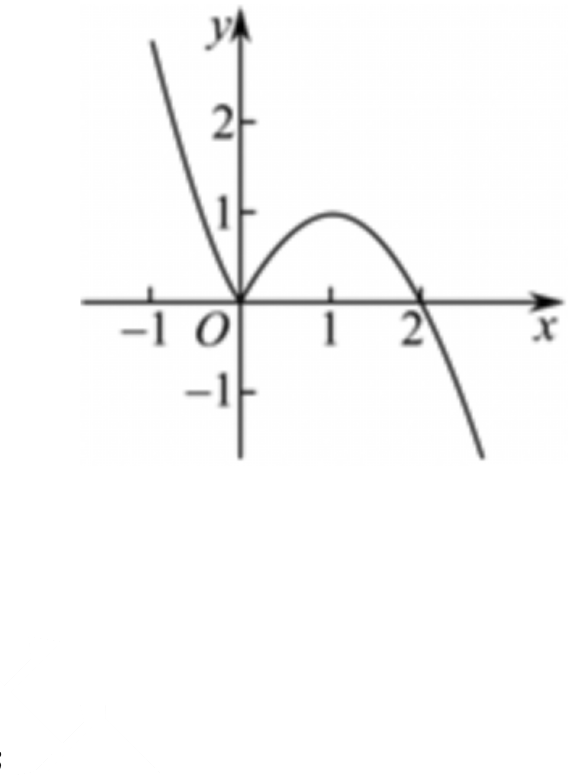
\includegraphics[width=0.20\textwidth]{figures/gao83_q15_graph.png}
\end{center}
\step{由 $[f(x)]^2+af(x)<0$ 得 $[f(x)+a]f(x)<0$，}
\step{当 $a=0$ 时，$[f(x)]^2<0$，不等式无解；}
\step{当 $a>0$ 时，由 $[f(x)+a]f(x)<0$ 得 $-a<f(x)<0$，}
\step{若不等式恰有 $1$ 个整数解，则整数解为 $3$，}
\step{又 $f(3)=-3$，$f(4)=-8$，所以 $-8\leqslant-a<-3$，所以 $3<a\leqslant8$；}
\step{当 $a<0$ 时，由 $[f(x)+a]f(x)<0$ 得 $0<f(x)<-a$，此时有多个解，故舍去；}
\step{综上所述，实数 $a$ 的取值范围为 $(3,8]$. 故选 $C$.}
\solend
\fi

\item 设函数 $f(x)=\begin{cases}\lvert2^x-1\rvert,&x\leqslant2\\ -x+7,&x>2\end{cases}$，若互不相等的实数 $a$、$b$、$c$ 满足 $f(a)=f(b)=f(c)$，
则 $2^a+2^b+2^c$ 的取值范围是\mbox{（\quad）}

\keepwithprev
A. $(8,9)$\qquad B. $(65,129)$\qquad C. $(64,128)$\qquad D. $(66,130)$

\ifanswer
\solbegin
\step{作出函数 $f(x)=\begin{cases}\lvert2^x-1\rvert,&x\leqslant2\\ -x+7,&x>2\end{cases}$ 的图象如图，}
\begin{center}
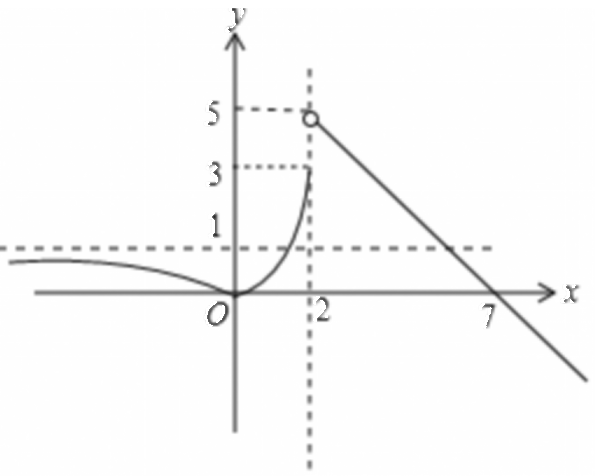
\includegraphics[width=0.22\textwidth]{figures/gao83_q16_graph.png}
\end{center}
\step{不妨设 $a<b<c$，由 $f(a)=f(b)$，得 $1-2^a=2^b-1$，则 $2^a+2^b=2$.}
\step{由 $f(-c)-c+6\in(0,1)$，得 $c\in(6,7)$，则 $64<2^c<128$，}
\step{所以 $66<2^a+2^b+2^c<130$，即 $2^a+2^b+2^c$ 的取值范围是 $(66,130)$. 故选 $D$.}
\solend
\fi

\end{enumerate}

\bigsec{三、解答题}

\begin{enumerate}
\setcounter{enumi}{16}

\item 已知幂函数 $f(x)$ 与一次函数 $g(x)$ 的图象都经过点 $(4,2)$，且 $f(9)=g(5)$.

（1）求 $f(x)$ 与 $g(x)$ 的解析式；

（2）求函数 $h(x)=g(x)-f(x)$ 在 $[0,4]$ 上的值域.

\ansspace*[8]

\ifanswer
\solbegin
\stepm{（1）}{设 $f(x)=x^\alpha$，$g(x)=kx+b$，则 $4^\alpha=2$，即 $\alpha=\dfrac12$，}
\step{$\begin{cases}4k+b=2\\ 3=5k+b\end{cases}$，则 $k=1$，$b=-2$，所以 $f(x)=\sqrt x$，$g(x)=x-2$；}
\stepm{（2）}{$h(x)=g(x)-f(x)=x-\sqrt x-2$，}
\step{令 $t=\sqrt x$，则 $t\in[0,2]$，原函数可化为 $p(t)=t^2-t-2$，}
\step{当 $t=\dfrac12$ 时，函数取得最小值 $-\dfrac94$，当 $t=2$ 时，函数取得最大值 $0$，}
\step{即函数值域为 $\left[-\dfrac94,0\right]$.}
\solend
\fi

\item 目前某县有 $100$ 万人. 经过 $x$ 年后为 $y$ 万人. 如果年平均增长率是 $1.2\%$. 请回答下列问题：

（1）写出 $y$ 关于 $x$ 的函数解析式.

（2）计算 $10$ 年后该县的人口总数（精确到 $0.1$ 万人）.

（3）计算大约多少年后该县的人口总数将达到 $120$ 万（精确到 $1$ 年）.

\ansspace*[9]

\ifanswer
\solbegin
\stepm{（1）}{当 $x=1$ 时，$y=100+100\times1.2\%=100(1+1.2\%)$，}
\step{当 $x=2$ 时，$y=100(1+1.2\%)+100(1+1.2\%)\times1.2\%=100(1+1.2\%)^2$，}
\step{当 $x=3$ 时，$y=100(1+1.2\%)^2+100(1+1.2\%)^2\times1.2\%=100(1+1.2\%)^3$，}
\step{$\cdots\cdots$}
\step{故 $y$ 关于 $x$ 的函数解析式为 $y=100(1+1.2\%)^x\,(x\in\N^*)$；}
\stepm{（2）}{当 $x=10$ 时，$y=100(1+1.2\%)^{10}=100\times1.012^{10}\approx112.7$，}
\step{故 $10$ 年后该县的人口总数约为 $112.7$ 万人；}
\stepm{（3）}{设 $x$ 年后该县的人口总数将达到 $120$ 万，即 $y=100(1+1.2\%)^x=120$，}
\step{解得 $x=\log_{1.012}\dfrac{120}{100}\approx16$，故大约 $16$ 年后该县的人口总数将达到 $120$ 万.}
\solend
\fi

\item 已知 $a>0$ 且 $a\neq1$，$m>0$，函数 $f(x)=(m^2+m-5)a^x$ 是指数函数，且 $f(2)=4$.

（1）求实数 $m$ 和 $a$ 的值；

（2）$f(2x)-2f(x)+2\geqslant nf(x)$ 对任意 $x\in[-1,2]$ 恒成立，求实数 $n$ 的取值范围；

（3）若关于 $x$ 的方程 $f(2x)-(2k+8)f(x)+2k+7b=0$ 有两个不相等的实数根，且一根
大于 $0$，另一根小于 $0$，其中 $k>0$，求整数 $b$ 的最大值.

\ansspace*[11]

\ifanswer
\solbegin
\stepm{（1）}{因为函数 $f(x)=(m^2+m-5)a^x$ 是指数函数，}
\step{所以 $m^2+m-5=1$，即 $m^2+m-6=0$，解得 $m=2$ 或 $m=-3$，}
\step{又 $m>0$，所以 $m=2$，又 $f(2)=a^2=4$，$a>0$ 且 $a\neq1$，所以 $a=2$；}
\stepm{（2）}{由（1）得 $f(x)=2^x$，}
\step{由题意 $2^{2x}-2\cdot2^x+2\geqslant n2^x$ 对任意 $x\in[-1,2]$ 恒成立，}
\step{所以 $n\leqslant2^x-2+\dfrac2{2^x}$ 对任意 $x\in[-1,2]$ 恒成立，则 $n\leqslant\left(2^x-2+\dfrac2{2^x}\right)_{\min}$，}
\step{记 $g(x)=2^x-2+\dfrac2{2^x}$，$x\in[-1,2]$，}
\step{令 $t=2^x$，因为 $x\in[-1,2]$，所以 $t\in\left[\dfrac12,4\right]$，则 $y=t+\dfrac2t-2$，$t\in\left[\dfrac12,4\right]$，}
\step{函数 $y=t+\dfrac2t-2$ 在 $\left[\dfrac12,\sqrt2\right]$ 上严格减，在 $[\sqrt2,4]$ 上严格增，}
\step{所以 $y=t+\dfrac2t-2$ 的最小值为 $\sqrt2+\dfrac2{\sqrt2}-2=2\sqrt2-2$，}
\step{所以 $n\leqslant2\sqrt2-2$，即实数 $n$ 的取值范围为 $(-\infty,2\sqrt2-2]$；}
\stepm{（3）}{方程 $f(2x)-(2k+8)f(x)+2k+7b=0$，}
\step{即方程 $2^{2x}-(2k+8)2^x+2k+7b=0$，即方程 $(2^x)^2-(2k+8)2^x+2k+7b=0$，}
\step{令 $t=2^x>0$，则方程 $t^2-(2k+8)t+2k+7b=0$，}
\step{因为关于 $x$ 的方程 $f(2x)-(2k+8)f(x)+2k+7b=0$ 的一根大于 $0$，另一根小于 $0$，}
\step{所以关于 $t$ 的方程 $t^2-(2k+8)t+2k+7b=0$ 的一根大于 $1$，另一根大于 $0$ 且小于 $1$，}
\step{记 $h(t)=t^2-(2k+8)t+2k+7b$，}
\step{所以 $\begin{cases}h(1)=1^2-(2k+8)\cdot1+2k+7b<0\\ h(0)=2k+7b>0\\ k>0\end{cases}$，所以 $\begin{cases}b<1\\ b>-\dfrac27k\\ k>0\end{cases}$，}
\step{所以整数 $b$ 的最大值为 $0$.}
\solend
\fi

\item 已知幂函数 $f(x)=(p^2-3p+3)x^{p^2-\frac32p-\frac12}$ 满足 $f(2)<f(4)$.

（1）求函数 $f(x)$ 的解析式；

（2）若函数 $g(x)=f^2(x)+mf(x)$，$x\in[1,9]$，是否存在实数 $m$ 使得 $g(x)$ 的最小值为 $0$？
若存在，求出 $m$ 的值；若不存在，说明理由.

（3）若函数 $h(x)=n-f(x+3)$，是否存在实数 $a$、$b\,(a<b)$，使函数 $h(x)$ 在 $[a,b]$ 上的
值域为 $[a,b]$？若存在，求出实数 $n$ 的取值范围；若不存在，说明理由.

\ansspace*[12]

\ifanswer
\solbegin
\stepm{（1）}{因为 $f(x)$ 是幂函数，所以 $p^2-3p+3=1$，解得 $p=1$ 或 $p=2$，}
\step{当 $p=1$ 时，$f(x)=\dfrac1x$，不满足 $f(2)<f(4)$.}
\step{当 $p=2$ 时，$f(x)=\sqrt x$，满足 $f(2)<f(4)$.}
\step{故 $p=2$，函数 $f(x)$ 的解析式为 $f(x)=\sqrt x$；}
\stepm{（2）}{由函数 $g(x)=f^2(x)+mf(x)$，即 $g(x)=(\sqrt x)^2+m\sqrt x$，}
\step{令 $t=\sqrt x$，因为 $x\in[1,9]$，所以 $t\in[1,3]$，}
\step{记 $k(x)=t^2+mt$，其对称轴 $t=-\dfrac m2$，}
\step{①当 $-\dfrac m2\leqslant1$，即 $m\geqslant-2$ 时，则 $k(x)_{\min}=k(1)=1+m=0$，解得 $m=-1$；}
\step{②当 $1<-\dfrac m2<3$ 时，即 $-6<m<-2$，则 $k(x)_{\min}=k\left(-\dfrac m2\right)=-\dfrac{m^2}4=0$，}
\step{解得 $m=0$，不满足，舍去；}
\step{③当 $-\dfrac m2\geqslant3$ 时，即 $m\leqslant-6$ 时，则 $k(x)_{\min}=k(3)=3m+9=0$，解得 $m=-3$，}
\step{不满足，舍去；}
\step{综上所述，存在 $m=-1$ 使得 $g(x)$ 的最小值为 $0$；}
\stepm{（3）}{由函数 $h(x)=n-f(x+3)=n-\sqrt{x+3}$ 在定义域内为严格减函数，}
\step{若存在实数 $a$、$b\,(a<b)$，使函数 $h(x)$ 在 $[a,b]$ 上的值域为 $[a,b]$，}
\step{则 $h(x)=\begin{cases}n-\sqrt{a+3}=b\text{ ①}\\ n-\sqrt{b+3}=a\text{ ②}\end{cases}$，}
\step{两式相减得 $\sqrt{a+3}-\sqrt{b+3}=a-b=(a+3)-(b+3)$，}
\step{所以 $\sqrt{a+3}+\sqrt{b+3}=1$ ③，}
\step{将③代入②得 $n=a+\sqrt{b+3}=a+1-\sqrt{a+3}$，}
\step{令 $t=\sqrt{a+3}$，因为 $a<b$，所以 $0\leqslant t<\dfrac12$，得 $n=t^2-t-2=\left(t-\dfrac12\right)^2-\dfrac94$，}
\step{故实数 $n$ 的取值范围为 $\left(-\dfrac94,-2\right]$.}
\solend
\fi

\item 定理（三角不等式），对于任意的 $a$、$b\in\R$，恒有 $\bigl\lvert\lvert a\rvert-\lvert b\rvert\bigr\rvert\leqslant\lvert a\pm b\rvert\leqslant\lvert a\rvert+\lvert b\rvert$. 定义：
已知 $n\in\N$ 且 $n\geqslant3$，对于有序数组 $a_1$、$a_2$、$\cdots$、$a_n$，称 $\lvert a_1-a_2\rvert+\lvert a_2-a_3\rvert+\cdots+\lvert a_{n-1}-a_n\rvert$
为有序数组 $a_1$、$a_2$、$\cdots$、$a_n$ 的波动距离，记作 $f(a_1,a_2,\cdots,a_n)$，即
$f(a_1,a_2,\cdots,a_n)=\lvert a_1-a_2\rvert+\lvert a_2-a_3\rvert+\cdots+\lvert a_{n-1}-a_n\rvert$，请根据上述信息解决以下几个问题：

（1）求函数 $y=\lvert x-2\rvert+\lvert x-4\rvert$ 的最小值，并指出函数取到最小值时 $x$ 的取值范围；

（2）①求有序数组 $2$、$5$、$3$、$4$ 的波动距离 $f(2,5,3,4)$；

②求证：若 $a$、$b$、$c$、$d\in\R$ 且 $a<b<c$，则 $f(a,b,c,d)\leqslant f(a,c,b,d)$；

（3）同理可证得命题“若 $a$、$b$、$c$、$d\in\R$ 且 $c<b<a$ 时，$f(a,b,c,d)\leqslant f(a,c,b,d)$”也
是真命题（注：该命题无需证明，需要时可直接使用）.

设两两不相等的四个实数 $a_1$、$a_2$、$a_3$、$a_4\in\{3^1,3^2,3^3,3^4\}$，求有序数组 $a_1$、$a_2$、$a_3$、$a_4$ 的
波动距离 $f(a_1,a_2,a_3,a_4)$ 的最大值.

\ansspace*[14]

\ifanswer
\solbegin
\stepm{（1）}{由三角不等式得 $\bigl\lvert\lvert a\rvert-\lvert b\rvert\bigr\rvert\leqslant\lvert a\pm b\rvert\leqslant\lvert a\rvert+\lvert b\rvert$，}
\step{当且仅当 $\lvert a+b\rvert^2=(\lvert a\rvert+\lvert b\rvert)^2$ 时，}
\step{即当 $-ab=\lvert ab\rvert$ 时，即当 $ab\leqslant0$ 时取等号，}
\step{由三角不等式得 $y=\lvert x-2\rvert+\lvert x-4\rvert\geqslant\lvert(x-2)-(x-4)\rvert=2$，}
\step{当且仅当 $(x-2)(x-4)\leqslant0$ 时，即 $2\leqslant x\leqslant4$ 时取等号，}
\step{因此，函数 $y=\lvert x-2\rvert+\lvert x-4\rvert$ 的最小值为 $2$，此时 $x$ 的取值范围是 $[2,4]$.}
\stepm{（2）}{①由题中定义得 $f(2,5,3,4)=\lvert2-5\rvert+\lvert5-3\rvert+\lvert3-4\rvert=6$；}
\step{②$f(a,b,c,d)-f(a,c,b,d)=\lvert a-b\rvert+\lvert c-d\rvert-\lvert a-c\rvert-\lvert b-d\rvert$，}
\step{因为 $a<b<c$，所以 $\lvert a-b\rvert-\lvert a-c\rvert=-\lvert b-c\rvert$，$\lvert c-d\rvert-\lvert b-d\rvert\leqslant\lvert b-c\rvert$，}
\step{所以 $f(a,b,c,d)-f(a,c,b,d)\leqslant0$，即 $f(a,b,c,d)\leqslant f(a,c,b,d)$，}
\stepm{（3）}{$f(a,b,c,d)=\lvert a-b\rvert+\lvert b-c\rvert+\lvert c-d\rvert$}
\step{$=\lvert d-c\rvert+\lvert c-b\rvert+\lvert b-a\rvert=f(d,c,b,a)$，}
\step{当 $f(a_1,a_2,a_3,a_4)$ 取得最大值时，$a_2=\max\{a_1,a_2,a_3\}$ 或 $a_2=\min\{a_1,a_2,a_3\}$，}
\step{同理 $a_3=\max\{a_2,a_3,a_4\}$ 或 $a_3=\min\{a_2,a_3,a_4\}$，}
\step{若 $a_2=\max\{a_1,a_2,a_3\}$，则 $a_2>a_3$，所以 $a_3=\min\{a_2,a_3,a_4\}$，}
\step{故 $f(a_1,a_2,a_3,a_4)=\lvert a_1-a_2\rvert+\lvert a_2-a_3\rvert+\lvert a_3-a_4\rvert=a_2-a_1+a_2-a_3+a_4-a_3$}
\step{$=2a_2+a_4-2a_3-a_1\leqslant2\times3^4+3^3-2\times3^1-3^2=174$，}
\step{当且仅当 $a_1=3^2$，$a_2=3^4$，$a_3=3^1$，$a_4=3^3$ 时取等号，}
\step{所以 $f(3^2,3^4,3^1,3^3)$ 为 $f(a_1,a_2,a_3,a_4)$ 的最大值，}
\step{若 $a_2=\min\{a_1,a_2,a_3\}$，则 $a_2<a_3$，所以 $a_3=\max\{a_2,a_3,a_4\}$，}
\step{同理可得 $f(3^3,3^4,3^1,3^2)$ 为 $f(a_1,a_2,a_3,a_4)$ 的最大值，}
\step{综上所述，$f(a_1,a_2,a_3,a_4)$ 的最大值为 $174$.}
\solend
\fi

\end{enumerate}

\end{document}
"
% 紧凑版：xelatex "\def\iscompact{1}% 高一83_交附闵行_周末作业10.23.tex
%   —— 高一上数学“2026-2027 年交附闵行高一上周末作业 10.23”（讲评版）
% 试卷版：xelatex 高一83_交附闵行_周末作业10.23.tex
% 答案版：xelatex "\def\isanswer{1}% 高一83_交附闵行_周末作业10.23.tex
%   —— 高一上数学“2026-2027 年交附闵行高一上周末作业 10.23”（讲评版）
% 试卷版：xelatex 高一83_交附闵行_周末作业10.23.tex
% 答案版：xelatex "\def\isanswer{1}\input{高一83_交附闵行_周末作业10.23.tex}"
% 紧凑版：xelatex "\def\iscompact{1}\input{高一83_交附闵行_周末作业10.23.tex}"
%
% 原始材料：微信公众号“魔都数学加油站”文章，连载“27学年高一83”；
% 原文标题“27学年高一83——2026-2027年上海市交附闵行高一上周末作业10.23”；
% 原文链接：https://mp.weixin.qq.com/s/t5AfTwQXg4Sj4i_Dl5rgXA。
% 页面标注发布时间 2026-10-26 20:15（上海）。
% 正文为 12 张 PNG 页（`原图/高一83_交附闵行_周末作业10.23/01..12.png`），
% 尺寸混排（第 1—8 页为 4762×6735，第 9—12 页为 2560×3620），均按页序读取。
%
% 篇幅与题号：原卷自第 3 题起编号（第 1、2 题不在原文内）。填空题 3—12（10 题）、
% 选择题 13—16（4 题）、解答题 17—21（5 题），共 19 题。
%
% 讲评版：19 题全部印【解析】，本稿不另提 \ans{}；选择题答案在解析末句“故选 C／B／C／D”。
%
% 副标题：原卷未印副标题。本稿按内容标作“函数与导数”（本卷考幂函数、指数函数、
% 对数与函数应用，属“函数与导数”模块；副标题只用知识模块名，见 README 说明）。
%
% 与原卷的排版差异：
%   ① 原卷每题下直接印【解析】，本稿按全稿惯例将解析置于答案版；
%   ② 原卷未印副标题，本稿补出；填空横线统一排 \blankline[4.4em]；
%   ③ 原卷数集记号排斜体 $R$、$Z$、$N$，本稿按全稿惯例改用 $\R$、$\Z$、$\N$；
%   ④ 第 17—21 题的子问用行内“（1）（2）（3）”段，解析中的子问标号用 \stepm；
%   ⑤ 解答题按惯例加 \ansspace；选择题括号排 \mbox{（\quad）}；
%   ⑥ 第 15、16 题解析各有一幅函数图象，裁自原图（第 6 页）后去粉色水印、转灰度，
%      仅答案版出。
%
% 行数核对：逐题数 \step/\stepm 条数，合计 145 条（Q3：1；Q4：1；Q5：4；Q6：5；
% Q7：2；Q8：7；Q9：10；Q10：5；Q11：6；Q12：8；Q13：3；Q14：4；Q15：8；
% Q16：4；Q17：6；Q18：9；Q19：19；Q20：21；Q21：22）。原卷解析的换行
% 按语意合并，未逐行强拆。
%
\documentclass[a4paper,11pt]{article}
\usepackage{common}

\begin{document}

\examtitlest[4]{2026--2027 年交附闵行高一上周末作业 10.23}{函数与导数}

\bigsec{一、填空题}

\begin{enumerate}
\setcounter{enumi}{2}

\item 已知 $10^a=2$，$10^b=5$，则 $10^{3a-2b}$ 的值为\blankline[4.4em].

\ifanswer
\solbegin
\step{$10^{3a-2b}=\dfrac{10^{3a}}{10^{2b}}=\dfrac{(10^a)^3}{(10^b)^2}=\dfrac{2^3}{5^2}=\dfrac8{25}$.}
\solend
\fi

\item 根式 $a\sqrt{-a}$ 化成分数指数幂是\blankline[4.4em].

\ifanswer
\solbegin
\step{$a\sqrt{-a}=a(-a)^{\frac12}=-(-a)(-a)^{\frac12}=-(-a)^{\frac32}$.}
\solend
\fi

\item 已知数列 $\{a_n\}$ 的通项公式为 $a_n=\left(\dfrac49\right)^{n-1}-\left(\dfrac23\right)^{n-1}$，在下列说法中：①有最大项；
②有最小项；③没有最大项；④没有最小项. 正确的是\blankline[3.6em]（填序号）.

\ifanswer
\solbegin
\step{令 $t=\left(\dfrac23\right)^{n-1}$，则 $t\in\left\{1,\dfrac23,\dfrac49,\dfrac8{27},\cdots\right\}\subset(0,1]$，$t$ 是关于 $n$ 的减函数，}
\step{则 $a_n=t^2-t=\left(t-\dfrac12\right)^2-\dfrac14$，}
\step{所以当 $t=1$ 即 $n=1$ 时 $a_n$ 取得最大为 $0$，当 $t=\dfrac49$ 即 $n=3$ 时 $a_n$ 取得最小为 $-\dfrac{20}{81}$，}
\step{所以 $a_n$ 既有最大项又有最小项，故①和②正确.}
\solend
\fi

\item 已知 $f(x)=\mathrm{e}^{x-\frac12}-\mathrm{e}^{-x+\frac12}+\dfrac{4x}{2x-1}$，则
$f\left(\dfrac1{2020}\right)+f\left(\dfrac2{2020}\right)+f\left(\dfrac3{2020}\right)+\cdots+f\left(\dfrac{1009}{2020}\right)+f\left(\dfrac{1011}{2020}\right)+\cdots+f\left(\dfrac{2019}{2020}\right)$ 的
值为\blankline[4.4em].

\ifanswer
\solbegin
\step{因为 $f(x)+f(1-x)=\mathrm{e}^{x-\frac12}-\mathrm{e}^{-x+\frac12}+\dfrac{4x}{2x-1}+\mathrm{e}^{(1-x)-\frac12}-\mathrm{e}^{-(1-x)+\frac12}+\dfrac{4(1-x)}{2(1-x)-1}$}
\step{$=\dfrac{4x}{2x-1}+\dfrac{4-4x}{1-2x}=\dfrac{4(2x-1)}{2x-1}=4$，}
\step{记 $S=f\left(\dfrac1{2020}\right)+f\left(\dfrac2{2020}\right)+\cdots+f\left(\dfrac{2019}{2020}\right)$，}
\step{又 $S=f\left(\dfrac{2019}{2020}\right)+f\left(\dfrac{2018}{2020}\right)+\cdots+f\left(\dfrac2{2020}\right)+f\left(\dfrac1{2020}\right)$，}
\step{对齐相加得 $2S=2018\times4$，所以 $S=4036$.}
\solend
\fi

\item 不等式 $2^{x^2-2x-3}<\left(\dfrac12\right)^{3(x-1)}$ 的解集为\blankline[4.4em].

\ifanswer
\solbegin
\step{由 $2^{x^2-2x-3}<\left(\dfrac12\right)^{3(x-1)}$ 得 $x^2-2x-3<-3(x-1)$，即 $x^2+x-6<0$，}
\step{故解集为 $(-3,2)$.}
\solend
\fi

\item 函数 $f(x)=x^{\ln5}+x^{\ln12}-13^{\ln x}$ 的零点是\blankline[4.4em]. 附：$a^{\log_bc}=c^{\log_ba}$
（$a>0$，$b>0$，$c>0$，$b\neq1$）.

\ifanswer
\solbegin
\step{函数 $f(x)=x^{\ln5}+x^{\ln12}-13^{\ln x}$，}
\step{若 $f(x)=x^{\ln5}+x^{\ln12}-13^{\ln x}=0$，变形得 $x^{\ln5}+x^{\ln12}=13^{\ln x}$，}
\step{又 $a^{\log_bc}=c^{\log_ba}$（$a>0$，$b>0$，$c>0$，$b\neq1$），得 $5^{\ln x}+12^{\ln x}=13^{\ln x}$，}
\step{令 $g(t)=\left(\dfrac5{13}\right)^t+\left(\dfrac{12}{13}\right)^t-1$，易得 $g(t)$ 严格减，所以 $g(t)=0$ 至多有一解，}
\step{即 $\left(\dfrac5{13}\right)^t+\left(\dfrac{12}{13}\right)^t-1=0$ 至多有一解，变形得方程 $5^t+12^t=13^t$ 至多有一解，}
\step{易得 $t=2$ 时，有 $5^2+12^2=13^2$ 成立，则方程 $5^t+12^t=13^t$ 有唯一解 $t=2$，}
\step{即 $\ln x=2$，解得 $x=\mathrm{e}^2$，即函数 $f(x)$ 的零点为 $\mathrm{e}^2$.}
\solend
\fi

\item 已知幂函数 $f(x)=(m^2-2m-2)x^{m^2+m-2}$ 在 $(0,+\infty)$ 上是严格减函数，则不等式
$f(x-1)<f(3-2x)$ 的解集为\blankline[4.4em].

\ifanswer
\solbegin
\step{因为 $f(x)$ 为幂函数，所以 $m^2-2m-2=1$，解得 $m=-1$ 或 $m=3$；}
\step{当 $m=3$ 时，$f(x)=x^{10}$ 在 $(0,+\infty)$ 上严格增，不合题意；}
\step{当 $m=-1$ 时，$f(x)=x^{-2}$ 在 $(0,+\infty)$ 上严格减，符合题意；}
\step{综上所述，$m=-1$；}
\step{因为 $f(x)=x^{-2}$ 的定义域为 $(-\infty,0)\cup(0,+\infty)$，$f(-x)=(-x)^{-2}=x^{-2}=f(x)$，}
\step{所以 $f(x)$ 为定义在 $(-\infty,0)\cup(0,+\infty)$ 上的偶函数，}
\step{故 $f(x-1)=f(\lvert x-1\rvert)$，$f(3-2x)=f(\lvert3-2x\rvert)$，}
\step{$f(x-1)<f(3-2x)\Rightarrow f(\lvert x-1\rvert)<f(\lvert3-2x\rvert)\Rightarrow\lvert x-1\rvert>\lvert3-2x\rvert$}
\step{且 $\lvert x-1\rvert\neq0$，$\lvert3-2x\rvert\neq0$，解得 $\dfrac43<x<\dfrac32$ 或 $\dfrac32<x<2$，}
\step{所以 $f(x-1)<f(3-2x)$ 的解集为 $\left(\dfrac43,\dfrac32\right)\cup\left(\dfrac32,2\right)$.}
\solend
\fi

\item 若实数 $x_1$、$x_2$ 满足 $\mathrm{e}^{x_1}+x_1-3=0$，$x_2\ln x_2+3x_2-1=0$，则 $\dfrac{x_1x_2+1}{x_2}$ 的值为\blankline[4.4em].

\ifanswer
\solbegin
\step{易得 $x_2>0$，则 $\ln x_2+3-\dfrac1{x_2}=0$，即 $\mathrm{e}^{-\ln x_2}+(-\ln x_2)-3=0$.}
\step{设 $f(x)=\mathrm{e}^x+x-3$，则函数 $f(x)$ 在 $(-\infty,+\infty)$ 上严格增.}
\step{由 $\mathrm{e}^{x_1}+x_1-3=0$，$\mathrm{e}^{-\ln x_2}+(-\ln x_2)-3=0$，得 $f(x_1)=0$，$f(-\ln x_2)=0$，}
\step{所以 $f(x_1)=f(-\ln x_2)$，得 $x_1=-\ln x_2$，即 $\ln x_2=-x_1$，所以 $x_2=\mathrm{e}^{-x_1}$，得 $\dfrac1{x_2}=\mathrm{e}^{x_1}$.}
\step{因为 $\mathrm{e}^{x_1}+x_1-3=0$，所以 $\mathrm{e}^{x_1}+x_1=3$，所以 $\dfrac{x_1x_2+1}{x_2}=x_1+\dfrac1{x_2}=\mathrm{e}^{x_1}+x_1=3$.}
\solend
\fi

\item 已知 $\alpha$、$\beta$ 是方程 $9^x-2m\cdot3^x+m^2-1=0$ 的两个根，若 $\alpha+\beta=1$，则 $\alpha\beta=\blankline[4.4em]$.

\ifanswer
\solbegin
\step{由题意得方程 $9^x-2m\cdot3^x+m^2-1=0$ 有两个根，}
\step{则方程 $t^2-2mt+m^2-1=0$ 有二正根，则 $\begin{cases}\Delta=4m^2-4(m^2-1)\geqslant0\\ 2m>0\\ m^2-1>0\end{cases}$，解得 $m>1$，}
\step{又 $\alpha$、$\beta$ 是方程 $9^x-2m\cdot3^x+m^2-1=0$ 的两个根，则 $3^\alpha\times3^\beta=m^2-1$，}
\step{又 $\alpha+\beta=1$，则 $m^2-1=3^{\alpha+\beta}=3$，解得 $m=2$ 或 $m=-2$（舍），}
\step{则 $3^\alpha+3^\beta=2m=4$，又 $\alpha=1-\beta$，则 $3^{1-\beta}+3^\beta=4$，解得 $\beta=0$ 或 $\beta=1$，}
\step{则 $\begin{cases}\alpha=1\\ \beta=0\end{cases}$ 或 $\begin{cases}\alpha=0\\ \beta=1\end{cases}$，则 $\alpha\beta=0$.}
\solend
\fi

\item 已知实数 $a,b,c\in(1,+\infty)$，满足 $a^{\log_ba}\cdot b^{\log_cb}\cdot c^{\log_ac}=100$，则 $abc$ 的最大值为\blankline[4.4em].

\ifanswer
\solbegin
\step{由换底公式得 $\log_ba=\dfrac{\ln a}{\ln b}$，$\log_cb=\dfrac{\ln b}{\ln c}$，$\log_ac=\dfrac{\ln c}{\ln a}$，}
\step{设 $X=\ln a$，$Y=\ln b$，$Z=\ln c$，得 $a=\mathrm{e}^X$，$b=\mathrm{e}^Y$，$c=\mathrm{e}^Z$，}
\step{代入得 $a^{\log_ba}\cdot b^{\log_cb}\cdot c^{\log_ac}=a^{\frac{\ln a}{\ln b}}\cdot b^{\frac{\ln b}{\ln c}}\cdot c^{\frac{\ln c}{\ln a}}=(\mathrm{e}^X)^{\frac XY}\cdot(\mathrm{e}^Y)^{\frac YZ}\cdot(\mathrm{e}^Z)^{\frac ZX}=100$，}
\step{即 $\mathrm{e}^{\frac{X^2}Y+\frac{Y^2}Z+\frac{Z^2}X}=100$，两边取对数得 $\dfrac{X^2}Y+\dfrac{Y^2}Z+\dfrac{Z^2}X=\ln100$.}
\step{由 $a,b,c\in(1,+\infty)$，得 $X>0$，$Y>0$，$Z>0$，}
\step{由柯西不等式，得 $\left(\dfrac{X^2}Y+\dfrac{Y^2}Z+\dfrac{Z^2}X\right)(X+Y+Z)\geqslant(X+Y+Z)^2$，}
\step{即 $X+Y+Z\leqslant\dfrac{X^2}Y+\dfrac{Y^2}Z+\dfrac{Z^2}X=\ln100$，当且仅当 $X=Y=Z$ 时取等号，}
\step{因此 $(X+Y+Z)_{\max}=\ln100$，所以 $(abc)_{\max}=\mathrm{e}^{(X+Y+Z)_{\max}}=\mathrm{e}^{\ln100}=100$.}
\solend
\fi

\end{enumerate}

\bigsec{二、选择题}

\begin{enumerate}
\setcounter{enumi}{12}

\item 已知集合 $A=\{x\mid x=2k,k\in\Z\}$，$B=\{x\mid x=4k+2,\,k\in\Z\}$，则 $A\cup B=\mbox{（\quad）}$

\keepwithprev
A. $B$\qquad B. $\R$\qquad C. $A$\qquad D. 以上都不是

\ifanswer
\solbegin
\step{$B=\{x\mid x=4k+2,k\in\Z\}=\{x\mid x=2(2k+1),k\in\Z\}$，它表示奇数的 $2$ 倍组成的集合，}
\step{$A=\{x\mid x=2k,k\in\Z\}$，即集合 $A$ 是整数的 $2$ 倍组成的集合，}
\step{则 $B\subseteq A$，则 $A\cup B=A$. 故选 $C$.}
\solend
\fi

\item 教室通风的目的是通过空气的流动，排出室内的污浊空气和致病微生物，降低室内二氧化碳和致病微生物的浓度，送进室外的新鲜空气. 按照国家标准，教室内空气中二氧化碳日平均最高容许浓度应小于等于 $0.1\%$. 经测定，刚下课时，空气中含有 $0.2\%$ 的二氧化碳，若开窗通风后教室内二氧化碳的浓度为 $y\%$，且 $y$ 随时间 $t$（单位：分钟）的变化规律可以用函数 $y=0.05+\lambda\mathrm{e}^{-\frac t{12}}\,(\lambda\in\R)$ 描述，则该教室内的二氧化碳浓度达到国家标准至少需要的时间为\mbox{（\quad）}

\keepwithprev
A. $10$ 分钟\qquad B. $14$ 分钟\qquad C. $15$ 分钟\qquad D. $20$ 分钟

\ifanswer
\solbegin
\step{由题意得，当 $t=0$ 时，$y=0.2$，即 $0.05+\lambda\mathrm{e}^0=0.2$，解得 $\lambda=0.15$，}
\step{所以 $y=0.05+0.15\mathrm{e}^{-\frac t{12}}$，由题意得 $0.05+0.15\mathrm{e}^{-\frac t{12}}\leqslant0.1$，即 $\mathrm{e}^{-\frac t{12}}\leqslant\dfrac13$，}
\step{两边取对数得 $-\dfrac t{12}\leqslant-\ln3$，所以 $t\geqslant12\ln3\approx13.2$，}
\step{所以该教室内的二氧化碳浓度达到国家标准至少需要的时间为 $14$ 分钟. 故选 $B$.}
\solend
\fi

\item 已知函数 $f(x)=\begin{cases}-x^2+2x,&x\geqslant0\\ x^2-2x,&x<0\end{cases}$，若关于 $x$ 的不等式 $[f(x)]^2+af(x)<0$ 恰有 $1$ 个整数
解，则实数 $a$ 的最大值为\mbox{（\quad）}

\keepwithprev
A. $-2$\qquad B. $3$\qquad C. $8$\qquad D. $9$

\ifanswer
\solbegin
\step{作出 $f(x)$ 的图象，如图所示：}
\begin{center}
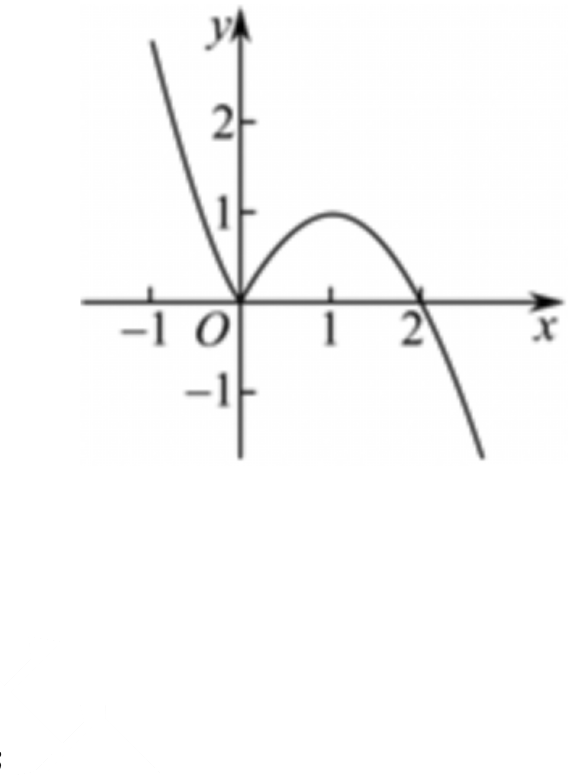
\includegraphics[width=0.20\textwidth]{figures/gao83_q15_graph.png}
\end{center}
\step{由 $[f(x)]^2+af(x)<0$ 得 $[f(x)+a]f(x)<0$，}
\step{当 $a=0$ 时，$[f(x)]^2<0$，不等式无解；}
\step{当 $a>0$ 时，由 $[f(x)+a]f(x)<0$ 得 $-a<f(x)<0$，}
\step{若不等式恰有 $1$ 个整数解，则整数解为 $3$，}
\step{又 $f(3)=-3$，$f(4)=-8$，所以 $-8\leqslant-a<-3$，所以 $3<a\leqslant8$；}
\step{当 $a<0$ 时，由 $[f(x)+a]f(x)<0$ 得 $0<f(x)<-a$，此时有多个解，故舍去；}
\step{综上所述，实数 $a$ 的取值范围为 $(3,8]$. 故选 $C$.}
\solend
\fi

\item 设函数 $f(x)=\begin{cases}\lvert2^x-1\rvert,&x\leqslant2\\ -x+7,&x>2\end{cases}$，若互不相等的实数 $a$、$b$、$c$ 满足 $f(a)=f(b)=f(c)$，
则 $2^a+2^b+2^c$ 的取值范围是\mbox{（\quad）}

\keepwithprev
A. $(8,9)$\qquad B. $(65,129)$\qquad C. $(64,128)$\qquad D. $(66,130)$

\ifanswer
\solbegin
\step{作出函数 $f(x)=\begin{cases}\lvert2^x-1\rvert,&x\leqslant2\\ -x+7,&x>2\end{cases}$ 的图象如图，}
\begin{center}
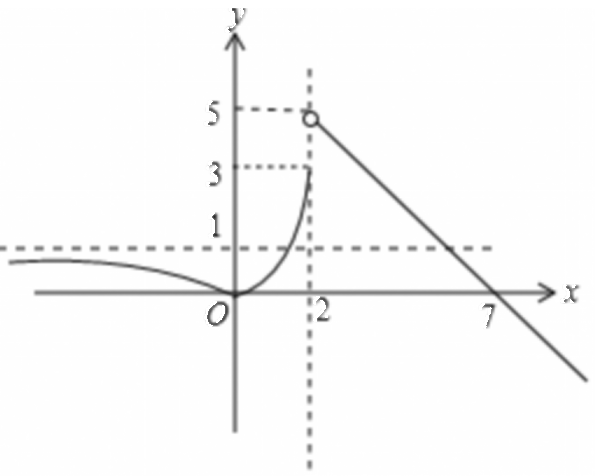
\includegraphics[width=0.22\textwidth]{figures/gao83_q16_graph.png}
\end{center}
\step{不妨设 $a<b<c$，由 $f(a)=f(b)$，得 $1-2^a=2^b-1$，则 $2^a+2^b=2$.}
\step{由 $f(-c)-c+6\in(0,1)$，得 $c\in(6,7)$，则 $64<2^c<128$，}
\step{所以 $66<2^a+2^b+2^c<130$，即 $2^a+2^b+2^c$ 的取值范围是 $(66,130)$. 故选 $D$.}
\solend
\fi

\end{enumerate}

\bigsec{三、解答题}

\begin{enumerate}
\setcounter{enumi}{16}

\item 已知幂函数 $f(x)$ 与一次函数 $g(x)$ 的图象都经过点 $(4,2)$，且 $f(9)=g(5)$.

（1）求 $f(x)$ 与 $g(x)$ 的解析式；

（2）求函数 $h(x)=g(x)-f(x)$ 在 $[0,4]$ 上的值域.

\ansspace*[8]

\ifanswer
\solbegin
\stepm{（1）}{设 $f(x)=x^\alpha$，$g(x)=kx+b$，则 $4^\alpha=2$，即 $\alpha=\dfrac12$，}
\step{$\begin{cases}4k+b=2\\ 3=5k+b\end{cases}$，则 $k=1$，$b=-2$，所以 $f(x)=\sqrt x$，$g(x)=x-2$；}
\stepm{（2）}{$h(x)=g(x)-f(x)=x-\sqrt x-2$，}
\step{令 $t=\sqrt x$，则 $t\in[0,2]$，原函数可化为 $p(t)=t^2-t-2$，}
\step{当 $t=\dfrac12$ 时，函数取得最小值 $-\dfrac94$，当 $t=2$ 时，函数取得最大值 $0$，}
\step{即函数值域为 $\left[-\dfrac94,0\right]$.}
\solend
\fi

\item 目前某县有 $100$ 万人. 经过 $x$ 年后为 $y$ 万人. 如果年平均增长率是 $1.2\%$. 请回答下列问题：

（1）写出 $y$ 关于 $x$ 的函数解析式.

（2）计算 $10$ 年后该县的人口总数（精确到 $0.1$ 万人）.

（3）计算大约多少年后该县的人口总数将达到 $120$ 万（精确到 $1$ 年）.

\ansspace*[9]

\ifanswer
\solbegin
\stepm{（1）}{当 $x=1$ 时，$y=100+100\times1.2\%=100(1+1.2\%)$，}
\step{当 $x=2$ 时，$y=100(1+1.2\%)+100(1+1.2\%)\times1.2\%=100(1+1.2\%)^2$，}
\step{当 $x=3$ 时，$y=100(1+1.2\%)^2+100(1+1.2\%)^2\times1.2\%=100(1+1.2\%)^3$，}
\step{$\cdots\cdots$}
\step{故 $y$ 关于 $x$ 的函数解析式为 $y=100(1+1.2\%)^x\,(x\in\N^*)$；}
\stepm{（2）}{当 $x=10$ 时，$y=100(1+1.2\%)^{10}=100\times1.012^{10}\approx112.7$，}
\step{故 $10$ 年后该县的人口总数约为 $112.7$ 万人；}
\stepm{（3）}{设 $x$ 年后该县的人口总数将达到 $120$ 万，即 $y=100(1+1.2\%)^x=120$，}
\step{解得 $x=\log_{1.012}\dfrac{120}{100}\approx16$，故大约 $16$ 年后该县的人口总数将达到 $120$ 万.}
\solend
\fi

\item 已知 $a>0$ 且 $a\neq1$，$m>0$，函数 $f(x)=(m^2+m-5)a^x$ 是指数函数，且 $f(2)=4$.

（1）求实数 $m$ 和 $a$ 的值；

（2）$f(2x)-2f(x)+2\geqslant nf(x)$ 对任意 $x\in[-1,2]$ 恒成立，求实数 $n$ 的取值范围；

（3）若关于 $x$ 的方程 $f(2x)-(2k+8)f(x)+2k+7b=0$ 有两个不相等的实数根，且一根
大于 $0$，另一根小于 $0$，其中 $k>0$，求整数 $b$ 的最大值.

\ansspace*[11]

\ifanswer
\solbegin
\stepm{（1）}{因为函数 $f(x)=(m^2+m-5)a^x$ 是指数函数，}
\step{所以 $m^2+m-5=1$，即 $m^2+m-6=0$，解得 $m=2$ 或 $m=-3$，}
\step{又 $m>0$，所以 $m=2$，又 $f(2)=a^2=4$，$a>0$ 且 $a\neq1$，所以 $a=2$；}
\stepm{（2）}{由（1）得 $f(x)=2^x$，}
\step{由题意 $2^{2x}-2\cdot2^x+2\geqslant n2^x$ 对任意 $x\in[-1,2]$ 恒成立，}
\step{所以 $n\leqslant2^x-2+\dfrac2{2^x}$ 对任意 $x\in[-1,2]$ 恒成立，则 $n\leqslant\left(2^x-2+\dfrac2{2^x}\right)_{\min}$，}
\step{记 $g(x)=2^x-2+\dfrac2{2^x}$，$x\in[-1,2]$，}
\step{令 $t=2^x$，因为 $x\in[-1,2]$，所以 $t\in\left[\dfrac12,4\right]$，则 $y=t+\dfrac2t-2$，$t\in\left[\dfrac12,4\right]$，}
\step{函数 $y=t+\dfrac2t-2$ 在 $\left[\dfrac12,\sqrt2\right]$ 上严格减，在 $[\sqrt2,4]$ 上严格增，}
\step{所以 $y=t+\dfrac2t-2$ 的最小值为 $\sqrt2+\dfrac2{\sqrt2}-2=2\sqrt2-2$，}
\step{所以 $n\leqslant2\sqrt2-2$，即实数 $n$ 的取值范围为 $(-\infty,2\sqrt2-2]$；}
\stepm{（3）}{方程 $f(2x)-(2k+8)f(x)+2k+7b=0$，}
\step{即方程 $2^{2x}-(2k+8)2^x+2k+7b=0$，即方程 $(2^x)^2-(2k+8)2^x+2k+7b=0$，}
\step{令 $t=2^x>0$，则方程 $t^2-(2k+8)t+2k+7b=0$，}
\step{因为关于 $x$ 的方程 $f(2x)-(2k+8)f(x)+2k+7b=0$ 的一根大于 $0$，另一根小于 $0$，}
\step{所以关于 $t$ 的方程 $t^2-(2k+8)t+2k+7b=0$ 的一根大于 $1$，另一根大于 $0$ 且小于 $1$，}
\step{记 $h(t)=t^2-(2k+8)t+2k+7b$，}
\step{所以 $\begin{cases}h(1)=1^2-(2k+8)\cdot1+2k+7b<0\\ h(0)=2k+7b>0\\ k>0\end{cases}$，所以 $\begin{cases}b<1\\ b>-\dfrac27k\\ k>0\end{cases}$，}
\step{所以整数 $b$ 的最大值为 $0$.}
\solend
\fi

\item 已知幂函数 $f(x)=(p^2-3p+3)x^{p^2-\frac32p-\frac12}$ 满足 $f(2)<f(4)$.

（1）求函数 $f(x)$ 的解析式；

（2）若函数 $g(x)=f^2(x)+mf(x)$，$x\in[1,9]$，是否存在实数 $m$ 使得 $g(x)$ 的最小值为 $0$？
若存在，求出 $m$ 的值；若不存在，说明理由.

（3）若函数 $h(x)=n-f(x+3)$，是否存在实数 $a$、$b\,(a<b)$，使函数 $h(x)$ 在 $[a,b]$ 上的
值域为 $[a,b]$？若存在，求出实数 $n$ 的取值范围；若不存在，说明理由.

\ansspace*[12]

\ifanswer
\solbegin
\stepm{（1）}{因为 $f(x)$ 是幂函数，所以 $p^2-3p+3=1$，解得 $p=1$ 或 $p=2$，}
\step{当 $p=1$ 时，$f(x)=\dfrac1x$，不满足 $f(2)<f(4)$.}
\step{当 $p=2$ 时，$f(x)=\sqrt x$，满足 $f(2)<f(4)$.}
\step{故 $p=2$，函数 $f(x)$ 的解析式为 $f(x)=\sqrt x$；}
\stepm{（2）}{由函数 $g(x)=f^2(x)+mf(x)$，即 $g(x)=(\sqrt x)^2+m\sqrt x$，}
\step{令 $t=\sqrt x$，因为 $x\in[1,9]$，所以 $t\in[1,3]$，}
\step{记 $k(x)=t^2+mt$，其对称轴 $t=-\dfrac m2$，}
\step{①当 $-\dfrac m2\leqslant1$，即 $m\geqslant-2$ 时，则 $k(x)_{\min}=k(1)=1+m=0$，解得 $m=-1$；}
\step{②当 $1<-\dfrac m2<3$ 时，即 $-6<m<-2$，则 $k(x)_{\min}=k\left(-\dfrac m2\right)=-\dfrac{m^2}4=0$，}
\step{解得 $m=0$，不满足，舍去；}
\step{③当 $-\dfrac m2\geqslant3$ 时，即 $m\leqslant-6$ 时，则 $k(x)_{\min}=k(3)=3m+9=0$，解得 $m=-3$，}
\step{不满足，舍去；}
\step{综上所述，存在 $m=-1$ 使得 $g(x)$ 的最小值为 $0$；}
\stepm{（3）}{由函数 $h(x)=n-f(x+3)=n-\sqrt{x+3}$ 在定义域内为严格减函数，}
\step{若存在实数 $a$、$b\,(a<b)$，使函数 $h(x)$ 在 $[a,b]$ 上的值域为 $[a,b]$，}
\step{则 $h(x)=\begin{cases}n-\sqrt{a+3}=b\text{ ①}\\ n-\sqrt{b+3}=a\text{ ②}\end{cases}$，}
\step{两式相减得 $\sqrt{a+3}-\sqrt{b+3}=a-b=(a+3)-(b+3)$，}
\step{所以 $\sqrt{a+3}+\sqrt{b+3}=1$ ③，}
\step{将③代入②得 $n=a+\sqrt{b+3}=a+1-\sqrt{a+3}$，}
\step{令 $t=\sqrt{a+3}$，因为 $a<b$，所以 $0\leqslant t<\dfrac12$，得 $n=t^2-t-2=\left(t-\dfrac12\right)^2-\dfrac94$，}
\step{故实数 $n$ 的取值范围为 $\left(-\dfrac94,-2\right]$.}
\solend
\fi

\item 定理（三角不等式），对于任意的 $a$、$b\in\R$，恒有 $\bigl\lvert\lvert a\rvert-\lvert b\rvert\bigr\rvert\leqslant\lvert a\pm b\rvert\leqslant\lvert a\rvert+\lvert b\rvert$. 定义：
已知 $n\in\N$ 且 $n\geqslant3$，对于有序数组 $a_1$、$a_2$、$\cdots$、$a_n$，称 $\lvert a_1-a_2\rvert+\lvert a_2-a_3\rvert+\cdots+\lvert a_{n-1}-a_n\rvert$
为有序数组 $a_1$、$a_2$、$\cdots$、$a_n$ 的波动距离，记作 $f(a_1,a_2,\cdots,a_n)$，即
$f(a_1,a_2,\cdots,a_n)=\lvert a_1-a_2\rvert+\lvert a_2-a_3\rvert+\cdots+\lvert a_{n-1}-a_n\rvert$，请根据上述信息解决以下几个问题：

（1）求函数 $y=\lvert x-2\rvert+\lvert x-4\rvert$ 的最小值，并指出函数取到最小值时 $x$ 的取值范围；

（2）①求有序数组 $2$、$5$、$3$、$4$ 的波动距离 $f(2,5,3,4)$；

②求证：若 $a$、$b$、$c$、$d\in\R$ 且 $a<b<c$，则 $f(a,b,c,d)\leqslant f(a,c,b,d)$；

（3）同理可证得命题“若 $a$、$b$、$c$、$d\in\R$ 且 $c<b<a$ 时，$f(a,b,c,d)\leqslant f(a,c,b,d)$”也
是真命题（注：该命题无需证明，需要时可直接使用）.

设两两不相等的四个实数 $a_1$、$a_2$、$a_3$、$a_4\in\{3^1,3^2,3^3,3^4\}$，求有序数组 $a_1$、$a_2$、$a_3$、$a_4$ 的
波动距离 $f(a_1,a_2,a_3,a_4)$ 的最大值.

\ansspace*[14]

\ifanswer
\solbegin
\stepm{（1）}{由三角不等式得 $\bigl\lvert\lvert a\rvert-\lvert b\rvert\bigr\rvert\leqslant\lvert a\pm b\rvert\leqslant\lvert a\rvert+\lvert b\rvert$，}
\step{当且仅当 $\lvert a+b\rvert^2=(\lvert a\rvert+\lvert b\rvert)^2$ 时，}
\step{即当 $-ab=\lvert ab\rvert$ 时，即当 $ab\leqslant0$ 时取等号，}
\step{由三角不等式得 $y=\lvert x-2\rvert+\lvert x-4\rvert\geqslant\lvert(x-2)-(x-4)\rvert=2$，}
\step{当且仅当 $(x-2)(x-4)\leqslant0$ 时，即 $2\leqslant x\leqslant4$ 时取等号，}
\step{因此，函数 $y=\lvert x-2\rvert+\lvert x-4\rvert$ 的最小值为 $2$，此时 $x$ 的取值范围是 $[2,4]$.}
\stepm{（2）}{①由题中定义得 $f(2,5,3,4)=\lvert2-5\rvert+\lvert5-3\rvert+\lvert3-4\rvert=6$；}
\step{②$f(a,b,c,d)-f(a,c,b,d)=\lvert a-b\rvert+\lvert c-d\rvert-\lvert a-c\rvert-\lvert b-d\rvert$，}
\step{因为 $a<b<c$，所以 $\lvert a-b\rvert-\lvert a-c\rvert=-\lvert b-c\rvert$，$\lvert c-d\rvert-\lvert b-d\rvert\leqslant\lvert b-c\rvert$，}
\step{所以 $f(a,b,c,d)-f(a,c,b,d)\leqslant0$，即 $f(a,b,c,d)\leqslant f(a,c,b,d)$，}
\stepm{（3）}{$f(a,b,c,d)=\lvert a-b\rvert+\lvert b-c\rvert+\lvert c-d\rvert$}
\step{$=\lvert d-c\rvert+\lvert c-b\rvert+\lvert b-a\rvert=f(d,c,b,a)$，}
\step{当 $f(a_1,a_2,a_3,a_4)$ 取得最大值时，$a_2=\max\{a_1,a_2,a_3\}$ 或 $a_2=\min\{a_1,a_2,a_3\}$，}
\step{同理 $a_3=\max\{a_2,a_3,a_4\}$ 或 $a_3=\min\{a_2,a_3,a_4\}$，}
\step{若 $a_2=\max\{a_1,a_2,a_3\}$，则 $a_2>a_3$，所以 $a_3=\min\{a_2,a_3,a_4\}$，}
\step{故 $f(a_1,a_2,a_3,a_4)=\lvert a_1-a_2\rvert+\lvert a_2-a_3\rvert+\lvert a_3-a_4\rvert=a_2-a_1+a_2-a_3+a_4-a_3$}
\step{$=2a_2+a_4-2a_3-a_1\leqslant2\times3^4+3^3-2\times3^1-3^2=174$，}
\step{当且仅当 $a_1=3^2$，$a_2=3^4$，$a_3=3^1$，$a_4=3^3$ 时取等号，}
\step{所以 $f(3^2,3^4,3^1,3^3)$ 为 $f(a_1,a_2,a_3,a_4)$ 的最大值，}
\step{若 $a_2=\min\{a_1,a_2,a_3\}$，则 $a_2<a_3$，所以 $a_3=\max\{a_2,a_3,a_4\}$，}
\step{同理可得 $f(3^3,3^4,3^1,3^2)$ 为 $f(a_1,a_2,a_3,a_4)$ 的最大值，}
\step{综上所述，$f(a_1,a_2,a_3,a_4)$ 的最大值为 $174$.}
\solend
\fi

\end{enumerate}

\end{document}
"
% 紧凑版：xelatex "\def\iscompact{1}% 高一83_交附闵行_周末作业10.23.tex
%   —— 高一上数学“2026-2027 年交附闵行高一上周末作业 10.23”（讲评版）
% 试卷版：xelatex 高一83_交附闵行_周末作业10.23.tex
% 答案版：xelatex "\def\isanswer{1}\input{高一83_交附闵行_周末作业10.23.tex}"
% 紧凑版：xelatex "\def\iscompact{1}\input{高一83_交附闵行_周末作业10.23.tex}"
%
% 原始材料：微信公众号“魔都数学加油站”文章，连载“27学年高一83”；
% 原文标题“27学年高一83——2026-2027年上海市交附闵行高一上周末作业10.23”；
% 原文链接：https://mp.weixin.qq.com/s/t5AfTwQXg4Sj4i_Dl5rgXA。
% 页面标注发布时间 2026-10-26 20:15（上海）。
% 正文为 12 张 PNG 页（`原图/高一83_交附闵行_周末作业10.23/01..12.png`），
% 尺寸混排（第 1—8 页为 4762×6735，第 9—12 页为 2560×3620），均按页序读取。
%
% 篇幅与题号：原卷自第 3 题起编号（第 1、2 题不在原文内）。填空题 3—12（10 题）、
% 选择题 13—16（4 题）、解答题 17—21（5 题），共 19 题。
%
% 讲评版：19 题全部印【解析】，本稿不另提 \ans{}；选择题答案在解析末句“故选 C／B／C／D”。
%
% 副标题：原卷未印副标题。本稿按内容标作“函数与导数”（本卷考幂函数、指数函数、
% 对数与函数应用，属“函数与导数”模块；副标题只用知识模块名，见 README 说明）。
%
% 与原卷的排版差异：
%   ① 原卷每题下直接印【解析】，本稿按全稿惯例将解析置于答案版；
%   ② 原卷未印副标题，本稿补出；填空横线统一排 \blankline[4.4em]；
%   ③ 原卷数集记号排斜体 $R$、$Z$、$N$，本稿按全稿惯例改用 $\R$、$\Z$、$\N$；
%   ④ 第 17—21 题的子问用行内“（1）（2）（3）”段，解析中的子问标号用 \stepm；
%   ⑤ 解答题按惯例加 \ansspace；选择题括号排 \mbox{（\quad）}；
%   ⑥ 第 15、16 题解析各有一幅函数图象，裁自原图（第 6 页）后去粉色水印、转灰度，
%      仅答案版出。
%
% 行数核对：逐题数 \step/\stepm 条数，合计 145 条（Q3：1；Q4：1；Q5：4；Q6：5；
% Q7：2；Q8：7；Q9：10；Q10：5；Q11：6；Q12：8；Q13：3；Q14：4；Q15：8；
% Q16：4；Q17：6；Q18：9；Q19：19；Q20：21；Q21：22）。原卷解析的换行
% 按语意合并，未逐行强拆。
%
\documentclass[a4paper,11pt]{article}
\usepackage{common}

\begin{document}

\examtitlest[4]{2026--2027 年交附闵行高一上周末作业 10.23}{函数与导数}

\bigsec{一、填空题}

\begin{enumerate}
\setcounter{enumi}{2}

\item 已知 $10^a=2$，$10^b=5$，则 $10^{3a-2b}$ 的值为\blankline[4.4em].

\ifanswer
\solbegin
\step{$10^{3a-2b}=\dfrac{10^{3a}}{10^{2b}}=\dfrac{(10^a)^3}{(10^b)^2}=\dfrac{2^3}{5^2}=\dfrac8{25}$.}
\solend
\fi

\item 根式 $a\sqrt{-a}$ 化成分数指数幂是\blankline[4.4em].

\ifanswer
\solbegin
\step{$a\sqrt{-a}=a(-a)^{\frac12}=-(-a)(-a)^{\frac12}=-(-a)^{\frac32}$.}
\solend
\fi

\item 已知数列 $\{a_n\}$ 的通项公式为 $a_n=\left(\dfrac49\right)^{n-1}-\left(\dfrac23\right)^{n-1}$，在下列说法中：①有最大项；
②有最小项；③没有最大项；④没有最小项. 正确的是\blankline[3.6em]（填序号）.

\ifanswer
\solbegin
\step{令 $t=\left(\dfrac23\right)^{n-1}$，则 $t\in\left\{1,\dfrac23,\dfrac49,\dfrac8{27},\cdots\right\}\subset(0,1]$，$t$ 是关于 $n$ 的减函数，}
\step{则 $a_n=t^2-t=\left(t-\dfrac12\right)^2-\dfrac14$，}
\step{所以当 $t=1$ 即 $n=1$ 时 $a_n$ 取得最大为 $0$，当 $t=\dfrac49$ 即 $n=3$ 时 $a_n$ 取得最小为 $-\dfrac{20}{81}$，}
\step{所以 $a_n$ 既有最大项又有最小项，故①和②正确.}
\solend
\fi

\item 已知 $f(x)=\mathrm{e}^{x-\frac12}-\mathrm{e}^{-x+\frac12}+\dfrac{4x}{2x-1}$，则
$f\left(\dfrac1{2020}\right)+f\left(\dfrac2{2020}\right)+f\left(\dfrac3{2020}\right)+\cdots+f\left(\dfrac{1009}{2020}\right)+f\left(\dfrac{1011}{2020}\right)+\cdots+f\left(\dfrac{2019}{2020}\right)$ 的
值为\blankline[4.4em].

\ifanswer
\solbegin
\step{因为 $f(x)+f(1-x)=\mathrm{e}^{x-\frac12}-\mathrm{e}^{-x+\frac12}+\dfrac{4x}{2x-1}+\mathrm{e}^{(1-x)-\frac12}-\mathrm{e}^{-(1-x)+\frac12}+\dfrac{4(1-x)}{2(1-x)-1}$}
\step{$=\dfrac{4x}{2x-1}+\dfrac{4-4x}{1-2x}=\dfrac{4(2x-1)}{2x-1}=4$，}
\step{记 $S=f\left(\dfrac1{2020}\right)+f\left(\dfrac2{2020}\right)+\cdots+f\left(\dfrac{2019}{2020}\right)$，}
\step{又 $S=f\left(\dfrac{2019}{2020}\right)+f\left(\dfrac{2018}{2020}\right)+\cdots+f\left(\dfrac2{2020}\right)+f\left(\dfrac1{2020}\right)$，}
\step{对齐相加得 $2S=2018\times4$，所以 $S=4036$.}
\solend
\fi

\item 不等式 $2^{x^2-2x-3}<\left(\dfrac12\right)^{3(x-1)}$ 的解集为\blankline[4.4em].

\ifanswer
\solbegin
\step{由 $2^{x^2-2x-3}<\left(\dfrac12\right)^{3(x-1)}$ 得 $x^2-2x-3<-3(x-1)$，即 $x^2+x-6<0$，}
\step{故解集为 $(-3,2)$.}
\solend
\fi

\item 函数 $f(x)=x^{\ln5}+x^{\ln12}-13^{\ln x}$ 的零点是\blankline[4.4em]. 附：$a^{\log_bc}=c^{\log_ba}$
（$a>0$，$b>0$，$c>0$，$b\neq1$）.

\ifanswer
\solbegin
\step{函数 $f(x)=x^{\ln5}+x^{\ln12}-13^{\ln x}$，}
\step{若 $f(x)=x^{\ln5}+x^{\ln12}-13^{\ln x}=0$，变形得 $x^{\ln5}+x^{\ln12}=13^{\ln x}$，}
\step{又 $a^{\log_bc}=c^{\log_ba}$（$a>0$，$b>0$，$c>0$，$b\neq1$），得 $5^{\ln x}+12^{\ln x}=13^{\ln x}$，}
\step{令 $g(t)=\left(\dfrac5{13}\right)^t+\left(\dfrac{12}{13}\right)^t-1$，易得 $g(t)$ 严格减，所以 $g(t)=0$ 至多有一解，}
\step{即 $\left(\dfrac5{13}\right)^t+\left(\dfrac{12}{13}\right)^t-1=0$ 至多有一解，变形得方程 $5^t+12^t=13^t$ 至多有一解，}
\step{易得 $t=2$ 时，有 $5^2+12^2=13^2$ 成立，则方程 $5^t+12^t=13^t$ 有唯一解 $t=2$，}
\step{即 $\ln x=2$，解得 $x=\mathrm{e}^2$，即函数 $f(x)$ 的零点为 $\mathrm{e}^2$.}
\solend
\fi

\item 已知幂函数 $f(x)=(m^2-2m-2)x^{m^2+m-2}$ 在 $(0,+\infty)$ 上是严格减函数，则不等式
$f(x-1)<f(3-2x)$ 的解集为\blankline[4.4em].

\ifanswer
\solbegin
\step{因为 $f(x)$ 为幂函数，所以 $m^2-2m-2=1$，解得 $m=-1$ 或 $m=3$；}
\step{当 $m=3$ 时，$f(x)=x^{10}$ 在 $(0,+\infty)$ 上严格增，不合题意；}
\step{当 $m=-1$ 时，$f(x)=x^{-2}$ 在 $(0,+\infty)$ 上严格减，符合题意；}
\step{综上所述，$m=-1$；}
\step{因为 $f(x)=x^{-2}$ 的定义域为 $(-\infty,0)\cup(0,+\infty)$，$f(-x)=(-x)^{-2}=x^{-2}=f(x)$，}
\step{所以 $f(x)$ 为定义在 $(-\infty,0)\cup(0,+\infty)$ 上的偶函数，}
\step{故 $f(x-1)=f(\lvert x-1\rvert)$，$f(3-2x)=f(\lvert3-2x\rvert)$，}
\step{$f(x-1)<f(3-2x)\Rightarrow f(\lvert x-1\rvert)<f(\lvert3-2x\rvert)\Rightarrow\lvert x-1\rvert>\lvert3-2x\rvert$}
\step{且 $\lvert x-1\rvert\neq0$，$\lvert3-2x\rvert\neq0$，解得 $\dfrac43<x<\dfrac32$ 或 $\dfrac32<x<2$，}
\step{所以 $f(x-1)<f(3-2x)$ 的解集为 $\left(\dfrac43,\dfrac32\right)\cup\left(\dfrac32,2\right)$.}
\solend
\fi

\item 若实数 $x_1$、$x_2$ 满足 $\mathrm{e}^{x_1}+x_1-3=0$，$x_2\ln x_2+3x_2-1=0$，则 $\dfrac{x_1x_2+1}{x_2}$ 的值为\blankline[4.4em].

\ifanswer
\solbegin
\step{易得 $x_2>0$，则 $\ln x_2+3-\dfrac1{x_2}=0$，即 $\mathrm{e}^{-\ln x_2}+(-\ln x_2)-3=0$.}
\step{设 $f(x)=\mathrm{e}^x+x-3$，则函数 $f(x)$ 在 $(-\infty,+\infty)$ 上严格增.}
\step{由 $\mathrm{e}^{x_1}+x_1-3=0$，$\mathrm{e}^{-\ln x_2}+(-\ln x_2)-3=0$，得 $f(x_1)=0$，$f(-\ln x_2)=0$，}
\step{所以 $f(x_1)=f(-\ln x_2)$，得 $x_1=-\ln x_2$，即 $\ln x_2=-x_1$，所以 $x_2=\mathrm{e}^{-x_1}$，得 $\dfrac1{x_2}=\mathrm{e}^{x_1}$.}
\step{因为 $\mathrm{e}^{x_1}+x_1-3=0$，所以 $\mathrm{e}^{x_1}+x_1=3$，所以 $\dfrac{x_1x_2+1}{x_2}=x_1+\dfrac1{x_2}=\mathrm{e}^{x_1}+x_1=3$.}
\solend
\fi

\item 已知 $\alpha$、$\beta$ 是方程 $9^x-2m\cdot3^x+m^2-1=0$ 的两个根，若 $\alpha+\beta=1$，则 $\alpha\beta=\blankline[4.4em]$.

\ifanswer
\solbegin
\step{由题意得方程 $9^x-2m\cdot3^x+m^2-1=0$ 有两个根，}
\step{则方程 $t^2-2mt+m^2-1=0$ 有二正根，则 $\begin{cases}\Delta=4m^2-4(m^2-1)\geqslant0\\ 2m>0\\ m^2-1>0\end{cases}$，解得 $m>1$，}
\step{又 $\alpha$、$\beta$ 是方程 $9^x-2m\cdot3^x+m^2-1=0$ 的两个根，则 $3^\alpha\times3^\beta=m^2-1$，}
\step{又 $\alpha+\beta=1$，则 $m^2-1=3^{\alpha+\beta}=3$，解得 $m=2$ 或 $m=-2$（舍），}
\step{则 $3^\alpha+3^\beta=2m=4$，又 $\alpha=1-\beta$，则 $3^{1-\beta}+3^\beta=4$，解得 $\beta=0$ 或 $\beta=1$，}
\step{则 $\begin{cases}\alpha=1\\ \beta=0\end{cases}$ 或 $\begin{cases}\alpha=0\\ \beta=1\end{cases}$，则 $\alpha\beta=0$.}
\solend
\fi

\item 已知实数 $a,b,c\in(1,+\infty)$，满足 $a^{\log_ba}\cdot b^{\log_cb}\cdot c^{\log_ac}=100$，则 $abc$ 的最大值为\blankline[4.4em].

\ifanswer
\solbegin
\step{由换底公式得 $\log_ba=\dfrac{\ln a}{\ln b}$，$\log_cb=\dfrac{\ln b}{\ln c}$，$\log_ac=\dfrac{\ln c}{\ln a}$，}
\step{设 $X=\ln a$，$Y=\ln b$，$Z=\ln c$，得 $a=\mathrm{e}^X$，$b=\mathrm{e}^Y$，$c=\mathrm{e}^Z$，}
\step{代入得 $a^{\log_ba}\cdot b^{\log_cb}\cdot c^{\log_ac}=a^{\frac{\ln a}{\ln b}}\cdot b^{\frac{\ln b}{\ln c}}\cdot c^{\frac{\ln c}{\ln a}}=(\mathrm{e}^X)^{\frac XY}\cdot(\mathrm{e}^Y)^{\frac YZ}\cdot(\mathrm{e}^Z)^{\frac ZX}=100$，}
\step{即 $\mathrm{e}^{\frac{X^2}Y+\frac{Y^2}Z+\frac{Z^2}X}=100$，两边取对数得 $\dfrac{X^2}Y+\dfrac{Y^2}Z+\dfrac{Z^2}X=\ln100$.}
\step{由 $a,b,c\in(1,+\infty)$，得 $X>0$，$Y>0$，$Z>0$，}
\step{由柯西不等式，得 $\left(\dfrac{X^2}Y+\dfrac{Y^2}Z+\dfrac{Z^2}X\right)(X+Y+Z)\geqslant(X+Y+Z)^2$，}
\step{即 $X+Y+Z\leqslant\dfrac{X^2}Y+\dfrac{Y^2}Z+\dfrac{Z^2}X=\ln100$，当且仅当 $X=Y=Z$ 时取等号，}
\step{因此 $(X+Y+Z)_{\max}=\ln100$，所以 $(abc)_{\max}=\mathrm{e}^{(X+Y+Z)_{\max}}=\mathrm{e}^{\ln100}=100$.}
\solend
\fi

\end{enumerate}

\bigsec{二、选择题}

\begin{enumerate}
\setcounter{enumi}{12}

\item 已知集合 $A=\{x\mid x=2k,k\in\Z\}$，$B=\{x\mid x=4k+2,\,k\in\Z\}$，则 $A\cup B=\mbox{（\quad）}$

\keepwithprev
A. $B$\qquad B. $\R$\qquad C. $A$\qquad D. 以上都不是

\ifanswer
\solbegin
\step{$B=\{x\mid x=4k+2,k\in\Z\}=\{x\mid x=2(2k+1),k\in\Z\}$，它表示奇数的 $2$ 倍组成的集合，}
\step{$A=\{x\mid x=2k,k\in\Z\}$，即集合 $A$ 是整数的 $2$ 倍组成的集合，}
\step{则 $B\subseteq A$，则 $A\cup B=A$. 故选 $C$.}
\solend
\fi

\item 教室通风的目的是通过空气的流动，排出室内的污浊空气和致病微生物，降低室内二氧化碳和致病微生物的浓度，送进室外的新鲜空气. 按照国家标准，教室内空气中二氧化碳日平均最高容许浓度应小于等于 $0.1\%$. 经测定，刚下课时，空气中含有 $0.2\%$ 的二氧化碳，若开窗通风后教室内二氧化碳的浓度为 $y\%$，且 $y$ 随时间 $t$（单位：分钟）的变化规律可以用函数 $y=0.05+\lambda\mathrm{e}^{-\frac t{12}}\,(\lambda\in\R)$ 描述，则该教室内的二氧化碳浓度达到国家标准至少需要的时间为\mbox{（\quad）}

\keepwithprev
A. $10$ 分钟\qquad B. $14$ 分钟\qquad C. $15$ 分钟\qquad D. $20$ 分钟

\ifanswer
\solbegin
\step{由题意得，当 $t=0$ 时，$y=0.2$，即 $0.05+\lambda\mathrm{e}^0=0.2$，解得 $\lambda=0.15$，}
\step{所以 $y=0.05+0.15\mathrm{e}^{-\frac t{12}}$，由题意得 $0.05+0.15\mathrm{e}^{-\frac t{12}}\leqslant0.1$，即 $\mathrm{e}^{-\frac t{12}}\leqslant\dfrac13$，}
\step{两边取对数得 $-\dfrac t{12}\leqslant-\ln3$，所以 $t\geqslant12\ln3\approx13.2$，}
\step{所以该教室内的二氧化碳浓度达到国家标准至少需要的时间为 $14$ 分钟. 故选 $B$.}
\solend
\fi

\item 已知函数 $f(x)=\begin{cases}-x^2+2x,&x\geqslant0\\ x^2-2x,&x<0\end{cases}$，若关于 $x$ 的不等式 $[f(x)]^2+af(x)<0$ 恰有 $1$ 个整数
解，则实数 $a$ 的最大值为\mbox{（\quad）}

\keepwithprev
A. $-2$\qquad B. $3$\qquad C. $8$\qquad D. $9$

\ifanswer
\solbegin
\step{作出 $f(x)$ 的图象，如图所示：}
\begin{center}
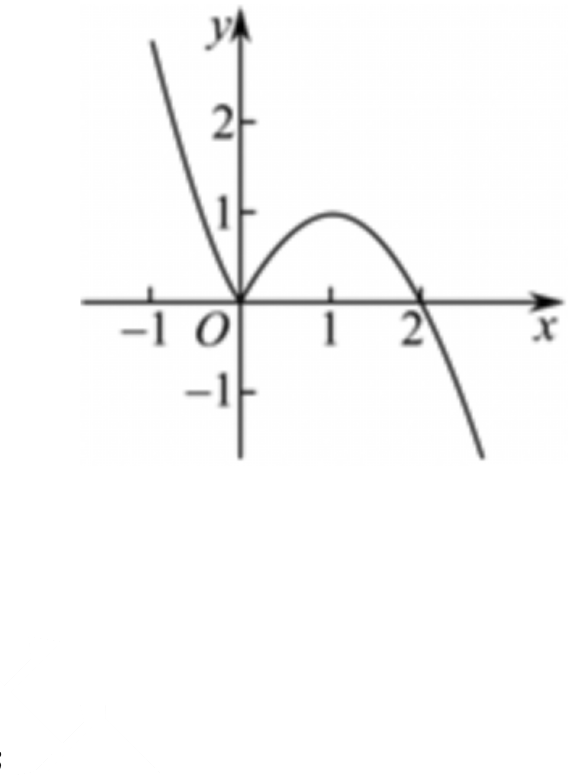
\includegraphics[width=0.20\textwidth]{figures/gao83_q15_graph.png}
\end{center}
\step{由 $[f(x)]^2+af(x)<0$ 得 $[f(x)+a]f(x)<0$，}
\step{当 $a=0$ 时，$[f(x)]^2<0$，不等式无解；}
\step{当 $a>0$ 时，由 $[f(x)+a]f(x)<0$ 得 $-a<f(x)<0$，}
\step{若不等式恰有 $1$ 个整数解，则整数解为 $3$，}
\step{又 $f(3)=-3$，$f(4)=-8$，所以 $-8\leqslant-a<-3$，所以 $3<a\leqslant8$；}
\step{当 $a<0$ 时，由 $[f(x)+a]f(x)<0$ 得 $0<f(x)<-a$，此时有多个解，故舍去；}
\step{综上所述，实数 $a$ 的取值范围为 $(3,8]$. 故选 $C$.}
\solend
\fi

\item 设函数 $f(x)=\begin{cases}\lvert2^x-1\rvert,&x\leqslant2\\ -x+7,&x>2\end{cases}$，若互不相等的实数 $a$、$b$、$c$ 满足 $f(a)=f(b)=f(c)$，
则 $2^a+2^b+2^c$ 的取值范围是\mbox{（\quad）}

\keepwithprev
A. $(8,9)$\qquad B. $(65,129)$\qquad C. $(64,128)$\qquad D. $(66,130)$

\ifanswer
\solbegin
\step{作出函数 $f(x)=\begin{cases}\lvert2^x-1\rvert,&x\leqslant2\\ -x+7,&x>2\end{cases}$ 的图象如图，}
\begin{center}
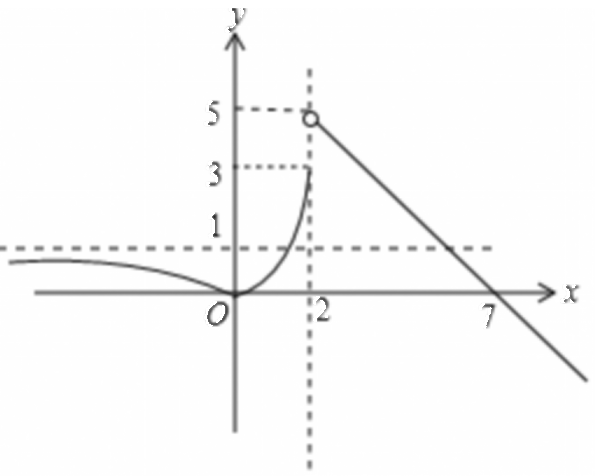
\includegraphics[width=0.22\textwidth]{figures/gao83_q16_graph.png}
\end{center}
\step{不妨设 $a<b<c$，由 $f(a)=f(b)$，得 $1-2^a=2^b-1$，则 $2^a+2^b=2$.}
\step{由 $f(-c)-c+6\in(0,1)$，得 $c\in(6,7)$，则 $64<2^c<128$，}
\step{所以 $66<2^a+2^b+2^c<130$，即 $2^a+2^b+2^c$ 的取值范围是 $(66,130)$. 故选 $D$.}
\solend
\fi

\end{enumerate}

\bigsec{三、解答题}

\begin{enumerate}
\setcounter{enumi}{16}

\item 已知幂函数 $f(x)$ 与一次函数 $g(x)$ 的图象都经过点 $(4,2)$，且 $f(9)=g(5)$.

（1）求 $f(x)$ 与 $g(x)$ 的解析式；

（2）求函数 $h(x)=g(x)-f(x)$ 在 $[0,4]$ 上的值域.

\ansspace*[8]

\ifanswer
\solbegin
\stepm{（1）}{设 $f(x)=x^\alpha$，$g(x)=kx+b$，则 $4^\alpha=2$，即 $\alpha=\dfrac12$，}
\step{$\begin{cases}4k+b=2\\ 3=5k+b\end{cases}$，则 $k=1$，$b=-2$，所以 $f(x)=\sqrt x$，$g(x)=x-2$；}
\stepm{（2）}{$h(x)=g(x)-f(x)=x-\sqrt x-2$，}
\step{令 $t=\sqrt x$，则 $t\in[0,2]$，原函数可化为 $p(t)=t^2-t-2$，}
\step{当 $t=\dfrac12$ 时，函数取得最小值 $-\dfrac94$，当 $t=2$ 时，函数取得最大值 $0$，}
\step{即函数值域为 $\left[-\dfrac94,0\right]$.}
\solend
\fi

\item 目前某县有 $100$ 万人. 经过 $x$ 年后为 $y$ 万人. 如果年平均增长率是 $1.2\%$. 请回答下列问题：

（1）写出 $y$ 关于 $x$ 的函数解析式.

（2）计算 $10$ 年后该县的人口总数（精确到 $0.1$ 万人）.

（3）计算大约多少年后该县的人口总数将达到 $120$ 万（精确到 $1$ 年）.

\ansspace*[9]

\ifanswer
\solbegin
\stepm{（1）}{当 $x=1$ 时，$y=100+100\times1.2\%=100(1+1.2\%)$，}
\step{当 $x=2$ 时，$y=100(1+1.2\%)+100(1+1.2\%)\times1.2\%=100(1+1.2\%)^2$，}
\step{当 $x=3$ 时，$y=100(1+1.2\%)^2+100(1+1.2\%)^2\times1.2\%=100(1+1.2\%)^3$，}
\step{$\cdots\cdots$}
\step{故 $y$ 关于 $x$ 的函数解析式为 $y=100(1+1.2\%)^x\,(x\in\N^*)$；}
\stepm{（2）}{当 $x=10$ 时，$y=100(1+1.2\%)^{10}=100\times1.012^{10}\approx112.7$，}
\step{故 $10$ 年后该县的人口总数约为 $112.7$ 万人；}
\stepm{（3）}{设 $x$ 年后该县的人口总数将达到 $120$ 万，即 $y=100(1+1.2\%)^x=120$，}
\step{解得 $x=\log_{1.012}\dfrac{120}{100}\approx16$，故大约 $16$ 年后该县的人口总数将达到 $120$ 万.}
\solend
\fi

\item 已知 $a>0$ 且 $a\neq1$，$m>0$，函数 $f(x)=(m^2+m-5)a^x$ 是指数函数，且 $f(2)=4$.

（1）求实数 $m$ 和 $a$ 的值；

（2）$f(2x)-2f(x)+2\geqslant nf(x)$ 对任意 $x\in[-1,2]$ 恒成立，求实数 $n$ 的取值范围；

（3）若关于 $x$ 的方程 $f(2x)-(2k+8)f(x)+2k+7b=0$ 有两个不相等的实数根，且一根
大于 $0$，另一根小于 $0$，其中 $k>0$，求整数 $b$ 的最大值.

\ansspace*[11]

\ifanswer
\solbegin
\stepm{（1）}{因为函数 $f(x)=(m^2+m-5)a^x$ 是指数函数，}
\step{所以 $m^2+m-5=1$，即 $m^2+m-6=0$，解得 $m=2$ 或 $m=-3$，}
\step{又 $m>0$，所以 $m=2$，又 $f(2)=a^2=4$，$a>0$ 且 $a\neq1$，所以 $a=2$；}
\stepm{（2）}{由（1）得 $f(x)=2^x$，}
\step{由题意 $2^{2x}-2\cdot2^x+2\geqslant n2^x$ 对任意 $x\in[-1,2]$ 恒成立，}
\step{所以 $n\leqslant2^x-2+\dfrac2{2^x}$ 对任意 $x\in[-1,2]$ 恒成立，则 $n\leqslant\left(2^x-2+\dfrac2{2^x}\right)_{\min}$，}
\step{记 $g(x)=2^x-2+\dfrac2{2^x}$，$x\in[-1,2]$，}
\step{令 $t=2^x$，因为 $x\in[-1,2]$，所以 $t\in\left[\dfrac12,4\right]$，则 $y=t+\dfrac2t-2$，$t\in\left[\dfrac12,4\right]$，}
\step{函数 $y=t+\dfrac2t-2$ 在 $\left[\dfrac12,\sqrt2\right]$ 上严格减，在 $[\sqrt2,4]$ 上严格增，}
\step{所以 $y=t+\dfrac2t-2$ 的最小值为 $\sqrt2+\dfrac2{\sqrt2}-2=2\sqrt2-2$，}
\step{所以 $n\leqslant2\sqrt2-2$，即实数 $n$ 的取值范围为 $(-\infty,2\sqrt2-2]$；}
\stepm{（3）}{方程 $f(2x)-(2k+8)f(x)+2k+7b=0$，}
\step{即方程 $2^{2x}-(2k+8)2^x+2k+7b=0$，即方程 $(2^x)^2-(2k+8)2^x+2k+7b=0$，}
\step{令 $t=2^x>0$，则方程 $t^2-(2k+8)t+2k+7b=0$，}
\step{因为关于 $x$ 的方程 $f(2x)-(2k+8)f(x)+2k+7b=0$ 的一根大于 $0$，另一根小于 $0$，}
\step{所以关于 $t$ 的方程 $t^2-(2k+8)t+2k+7b=0$ 的一根大于 $1$，另一根大于 $0$ 且小于 $1$，}
\step{记 $h(t)=t^2-(2k+8)t+2k+7b$，}
\step{所以 $\begin{cases}h(1)=1^2-(2k+8)\cdot1+2k+7b<0\\ h(0)=2k+7b>0\\ k>0\end{cases}$，所以 $\begin{cases}b<1\\ b>-\dfrac27k\\ k>0\end{cases}$，}
\step{所以整数 $b$ 的最大值为 $0$.}
\solend
\fi

\item 已知幂函数 $f(x)=(p^2-3p+3)x^{p^2-\frac32p-\frac12}$ 满足 $f(2)<f(4)$.

（1）求函数 $f(x)$ 的解析式；

（2）若函数 $g(x)=f^2(x)+mf(x)$，$x\in[1,9]$，是否存在实数 $m$ 使得 $g(x)$ 的最小值为 $0$？
若存在，求出 $m$ 的值；若不存在，说明理由.

（3）若函数 $h(x)=n-f(x+3)$，是否存在实数 $a$、$b\,(a<b)$，使函数 $h(x)$ 在 $[a,b]$ 上的
值域为 $[a,b]$？若存在，求出实数 $n$ 的取值范围；若不存在，说明理由.

\ansspace*[12]

\ifanswer
\solbegin
\stepm{（1）}{因为 $f(x)$ 是幂函数，所以 $p^2-3p+3=1$，解得 $p=1$ 或 $p=2$，}
\step{当 $p=1$ 时，$f(x)=\dfrac1x$，不满足 $f(2)<f(4)$.}
\step{当 $p=2$ 时，$f(x)=\sqrt x$，满足 $f(2)<f(4)$.}
\step{故 $p=2$，函数 $f(x)$ 的解析式为 $f(x)=\sqrt x$；}
\stepm{（2）}{由函数 $g(x)=f^2(x)+mf(x)$，即 $g(x)=(\sqrt x)^2+m\sqrt x$，}
\step{令 $t=\sqrt x$，因为 $x\in[1,9]$，所以 $t\in[1,3]$，}
\step{记 $k(x)=t^2+mt$，其对称轴 $t=-\dfrac m2$，}
\step{①当 $-\dfrac m2\leqslant1$，即 $m\geqslant-2$ 时，则 $k(x)_{\min}=k(1)=1+m=0$，解得 $m=-1$；}
\step{②当 $1<-\dfrac m2<3$ 时，即 $-6<m<-2$，则 $k(x)_{\min}=k\left(-\dfrac m2\right)=-\dfrac{m^2}4=0$，}
\step{解得 $m=0$，不满足，舍去；}
\step{③当 $-\dfrac m2\geqslant3$ 时，即 $m\leqslant-6$ 时，则 $k(x)_{\min}=k(3)=3m+9=0$，解得 $m=-3$，}
\step{不满足，舍去；}
\step{综上所述，存在 $m=-1$ 使得 $g(x)$ 的最小值为 $0$；}
\stepm{（3）}{由函数 $h(x)=n-f(x+3)=n-\sqrt{x+3}$ 在定义域内为严格减函数，}
\step{若存在实数 $a$、$b\,(a<b)$，使函数 $h(x)$ 在 $[a,b]$ 上的值域为 $[a,b]$，}
\step{则 $h(x)=\begin{cases}n-\sqrt{a+3}=b\text{ ①}\\ n-\sqrt{b+3}=a\text{ ②}\end{cases}$，}
\step{两式相减得 $\sqrt{a+3}-\sqrt{b+3}=a-b=(a+3)-(b+3)$，}
\step{所以 $\sqrt{a+3}+\sqrt{b+3}=1$ ③，}
\step{将③代入②得 $n=a+\sqrt{b+3}=a+1-\sqrt{a+3}$，}
\step{令 $t=\sqrt{a+3}$，因为 $a<b$，所以 $0\leqslant t<\dfrac12$，得 $n=t^2-t-2=\left(t-\dfrac12\right)^2-\dfrac94$，}
\step{故实数 $n$ 的取值范围为 $\left(-\dfrac94,-2\right]$.}
\solend
\fi

\item 定理（三角不等式），对于任意的 $a$、$b\in\R$，恒有 $\bigl\lvert\lvert a\rvert-\lvert b\rvert\bigr\rvert\leqslant\lvert a\pm b\rvert\leqslant\lvert a\rvert+\lvert b\rvert$. 定义：
已知 $n\in\N$ 且 $n\geqslant3$，对于有序数组 $a_1$、$a_2$、$\cdots$、$a_n$，称 $\lvert a_1-a_2\rvert+\lvert a_2-a_3\rvert+\cdots+\lvert a_{n-1}-a_n\rvert$
为有序数组 $a_1$、$a_2$、$\cdots$、$a_n$ 的波动距离，记作 $f(a_1,a_2,\cdots,a_n)$，即
$f(a_1,a_2,\cdots,a_n)=\lvert a_1-a_2\rvert+\lvert a_2-a_3\rvert+\cdots+\lvert a_{n-1}-a_n\rvert$，请根据上述信息解决以下几个问题：

（1）求函数 $y=\lvert x-2\rvert+\lvert x-4\rvert$ 的最小值，并指出函数取到最小值时 $x$ 的取值范围；

（2）①求有序数组 $2$、$5$、$3$、$4$ 的波动距离 $f(2,5,3,4)$；

②求证：若 $a$、$b$、$c$、$d\in\R$ 且 $a<b<c$，则 $f(a,b,c,d)\leqslant f(a,c,b,d)$；

（3）同理可证得命题“若 $a$、$b$、$c$、$d\in\R$ 且 $c<b<a$ 时，$f(a,b,c,d)\leqslant f(a,c,b,d)$”也
是真命题（注：该命题无需证明，需要时可直接使用）.

设两两不相等的四个实数 $a_1$、$a_2$、$a_3$、$a_4\in\{3^1,3^2,3^3,3^4\}$，求有序数组 $a_1$、$a_2$、$a_3$、$a_4$ 的
波动距离 $f(a_1,a_2,a_3,a_4)$ 的最大值.

\ansspace*[14]

\ifanswer
\solbegin
\stepm{（1）}{由三角不等式得 $\bigl\lvert\lvert a\rvert-\lvert b\rvert\bigr\rvert\leqslant\lvert a\pm b\rvert\leqslant\lvert a\rvert+\lvert b\rvert$，}
\step{当且仅当 $\lvert a+b\rvert^2=(\lvert a\rvert+\lvert b\rvert)^2$ 时，}
\step{即当 $-ab=\lvert ab\rvert$ 时，即当 $ab\leqslant0$ 时取等号，}
\step{由三角不等式得 $y=\lvert x-2\rvert+\lvert x-4\rvert\geqslant\lvert(x-2)-(x-4)\rvert=2$，}
\step{当且仅当 $(x-2)(x-4)\leqslant0$ 时，即 $2\leqslant x\leqslant4$ 时取等号，}
\step{因此，函数 $y=\lvert x-2\rvert+\lvert x-4\rvert$ 的最小值为 $2$，此时 $x$ 的取值范围是 $[2,4]$.}
\stepm{（2）}{①由题中定义得 $f(2,5,3,4)=\lvert2-5\rvert+\lvert5-3\rvert+\lvert3-4\rvert=6$；}
\step{②$f(a,b,c,d)-f(a,c,b,d)=\lvert a-b\rvert+\lvert c-d\rvert-\lvert a-c\rvert-\lvert b-d\rvert$，}
\step{因为 $a<b<c$，所以 $\lvert a-b\rvert-\lvert a-c\rvert=-\lvert b-c\rvert$，$\lvert c-d\rvert-\lvert b-d\rvert\leqslant\lvert b-c\rvert$，}
\step{所以 $f(a,b,c,d)-f(a,c,b,d)\leqslant0$，即 $f(a,b,c,d)\leqslant f(a,c,b,d)$，}
\stepm{（3）}{$f(a,b,c,d)=\lvert a-b\rvert+\lvert b-c\rvert+\lvert c-d\rvert$}
\step{$=\lvert d-c\rvert+\lvert c-b\rvert+\lvert b-a\rvert=f(d,c,b,a)$，}
\step{当 $f(a_1,a_2,a_3,a_4)$ 取得最大值时，$a_2=\max\{a_1,a_2,a_3\}$ 或 $a_2=\min\{a_1,a_2,a_3\}$，}
\step{同理 $a_3=\max\{a_2,a_3,a_4\}$ 或 $a_3=\min\{a_2,a_3,a_4\}$，}
\step{若 $a_2=\max\{a_1,a_2,a_3\}$，则 $a_2>a_3$，所以 $a_3=\min\{a_2,a_3,a_4\}$，}
\step{故 $f(a_1,a_2,a_3,a_4)=\lvert a_1-a_2\rvert+\lvert a_2-a_3\rvert+\lvert a_3-a_4\rvert=a_2-a_1+a_2-a_3+a_4-a_3$}
\step{$=2a_2+a_4-2a_3-a_1\leqslant2\times3^4+3^3-2\times3^1-3^2=174$，}
\step{当且仅当 $a_1=3^2$，$a_2=3^4$，$a_3=3^1$，$a_4=3^3$ 时取等号，}
\step{所以 $f(3^2,3^4,3^1,3^3)$ 为 $f(a_1,a_2,a_3,a_4)$ 的最大值，}
\step{若 $a_2=\min\{a_1,a_2,a_3\}$，则 $a_2<a_3$，所以 $a_3=\max\{a_2,a_3,a_4\}$，}
\step{同理可得 $f(3^3,3^4,3^1,3^2)$ 为 $f(a_1,a_2,a_3,a_4)$ 的最大值，}
\step{综上所述，$f(a_1,a_2,a_3,a_4)$ 的最大值为 $174$.}
\solend
\fi

\end{enumerate}

\end{document}
"
%
% 原始材料：微信公众号“魔都数学加油站”文章，连载“27学年高一83”；
% 原文标题“27学年高一83——2026-2027年上海市交附闵行高一上周末作业10.23”；
% 原文链接：https://mp.weixin.qq.com/s/t5AfTwQXg4Sj4i_Dl5rgXA。
% 页面标注发布时间 2026-10-26 20:15（上海）。
% 正文为 12 张 PNG 页（`原图/高一83_交附闵行_周末作业10.23/01..12.png`），
% 尺寸混排（第 1—8 页为 4762×6735，第 9—12 页为 2560×3620），均按页序读取。
%
% 篇幅与题号：原卷自第 3 题起编号（第 1、2 题不在原文内）。填空题 3—12（10 题）、
% 选择题 13—16（4 题）、解答题 17—21（5 题），共 19 题。
%
% 讲评版：19 题全部印【解析】，本稿不另提 \ans{}；选择题答案在解析末句“故选 C／B／C／D”。
%
% 副标题：原卷未印副标题。本稿按内容标作“函数与导数”（本卷考幂函数、指数函数、
% 对数与函数应用，属“函数与导数”模块；副标题只用知识模块名，见 README 说明）。
%
% 与原卷的排版差异：
%   ① 原卷每题下直接印【解析】，本稿按全稿惯例将解析置于答案版；
%   ② 原卷未印副标题，本稿补出；填空横线统一排 \blankline[4.4em]；
%   ③ 原卷数集记号排斜体 $R$、$Z$、$N$，本稿按全稿惯例改用 $\R$、$\Z$、$\N$；
%   ④ 第 17—21 题的子问用行内“（1）（2）（3）”段，解析中的子问标号用 \stepm；
%   ⑤ 解答题按惯例加 \ansspace；选择题括号排 \mbox{（\quad）}；
%   ⑥ 第 15、16 题解析各有一幅函数图象，裁自原图（第 6 页）后去粉色水印、转灰度，
%      仅答案版出。
%
% 行数核对：逐题数 \step/\stepm 条数，合计 145 条（Q3：1；Q4：1；Q5：4；Q6：5；
% Q7：2；Q8：7；Q9：10；Q10：5；Q11：6；Q12：8；Q13：3；Q14：4；Q15：8；
% Q16：4；Q17：6；Q18：9；Q19：19；Q20：21；Q21：22）。原卷解析的换行
% 按语意合并，未逐行强拆。
%
\documentclass[a4paper,11pt]{article}
\usepackage{common}

\begin{document}

\examtitlest[4]{2026--2027 年交附闵行高一上周末作业 10.23}{函数与导数}

\bigsec{一、填空题}

\begin{enumerate}
\setcounter{enumi}{2}

\item 已知 $10^a=2$，$10^b=5$，则 $10^{3a-2b}$ 的值为\blankline[4.4em].

\ifanswer
\solbegin
\step{$10^{3a-2b}=\dfrac{10^{3a}}{10^{2b}}=\dfrac{(10^a)^3}{(10^b)^2}=\dfrac{2^3}{5^2}=\dfrac8{25}$.}
\solend
\fi

\item 根式 $a\sqrt{-a}$ 化成分数指数幂是\blankline[4.4em].

\ifanswer
\solbegin
\step{$a\sqrt{-a}=a(-a)^{\frac12}=-(-a)(-a)^{\frac12}=-(-a)^{\frac32}$.}
\solend
\fi

\item 已知数列 $\{a_n\}$ 的通项公式为 $a_n=\left(\dfrac49\right)^{n-1}-\left(\dfrac23\right)^{n-1}$，在下列说法中：①有最大项；
②有最小项；③没有最大项；④没有最小项. 正确的是\blankline[3.6em]（填序号）.

\ifanswer
\solbegin
\step{令 $t=\left(\dfrac23\right)^{n-1}$，则 $t\in\left\{1,\dfrac23,\dfrac49,\dfrac8{27},\cdots\right\}\subset(0,1]$，$t$ 是关于 $n$ 的减函数，}
\step{则 $a_n=t^2-t=\left(t-\dfrac12\right)^2-\dfrac14$，}
\step{所以当 $t=1$ 即 $n=1$ 时 $a_n$ 取得最大为 $0$，当 $t=\dfrac49$ 即 $n=3$ 时 $a_n$ 取得最小为 $-\dfrac{20}{81}$，}
\step{所以 $a_n$ 既有最大项又有最小项，故①和②正确.}
\solend
\fi

\item 已知 $f(x)=\mathrm{e}^{x-\frac12}-\mathrm{e}^{-x+\frac12}+\dfrac{4x}{2x-1}$，则
$f\left(\dfrac1{2020}\right)+f\left(\dfrac2{2020}\right)+f\left(\dfrac3{2020}\right)+\cdots+f\left(\dfrac{1009}{2020}\right)+f\left(\dfrac{1011}{2020}\right)+\cdots+f\left(\dfrac{2019}{2020}\right)$ 的
值为\blankline[4.4em].

\ifanswer
\solbegin
\step{因为 $f(x)+f(1-x)=\mathrm{e}^{x-\frac12}-\mathrm{e}^{-x+\frac12}+\dfrac{4x}{2x-1}+\mathrm{e}^{(1-x)-\frac12}-\mathrm{e}^{-(1-x)+\frac12}+\dfrac{4(1-x)}{2(1-x)-1}$}
\step{$=\dfrac{4x}{2x-1}+\dfrac{4-4x}{1-2x}=\dfrac{4(2x-1)}{2x-1}=4$，}
\step{记 $S=f\left(\dfrac1{2020}\right)+f\left(\dfrac2{2020}\right)+\cdots+f\left(\dfrac{2019}{2020}\right)$，}
\step{又 $S=f\left(\dfrac{2019}{2020}\right)+f\left(\dfrac{2018}{2020}\right)+\cdots+f\left(\dfrac2{2020}\right)+f\left(\dfrac1{2020}\right)$，}
\step{对齐相加得 $2S=2018\times4$，所以 $S=4036$.}
\solend
\fi

\item 不等式 $2^{x^2-2x-3}<\left(\dfrac12\right)^{3(x-1)}$ 的解集为\blankline[4.4em].

\ifanswer
\solbegin
\step{由 $2^{x^2-2x-3}<\left(\dfrac12\right)^{3(x-1)}$ 得 $x^2-2x-3<-3(x-1)$，即 $x^2+x-6<0$，}
\step{故解集为 $(-3,2)$.}
\solend
\fi

\item 函数 $f(x)=x^{\ln5}+x^{\ln12}-13^{\ln x}$ 的零点是\blankline[4.4em]. 附：$a^{\log_bc}=c^{\log_ba}$
（$a>0$，$b>0$，$c>0$，$b\neq1$）.

\ifanswer
\solbegin
\step{函数 $f(x)=x^{\ln5}+x^{\ln12}-13^{\ln x}$，}
\step{若 $f(x)=x^{\ln5}+x^{\ln12}-13^{\ln x}=0$，变形得 $x^{\ln5}+x^{\ln12}=13^{\ln x}$，}
\step{又 $a^{\log_bc}=c^{\log_ba}$（$a>0$，$b>0$，$c>0$，$b\neq1$），得 $5^{\ln x}+12^{\ln x}=13^{\ln x}$，}
\step{令 $g(t)=\left(\dfrac5{13}\right)^t+\left(\dfrac{12}{13}\right)^t-1$，易得 $g(t)$ 严格减，所以 $g(t)=0$ 至多有一解，}
\step{即 $\left(\dfrac5{13}\right)^t+\left(\dfrac{12}{13}\right)^t-1=0$ 至多有一解，变形得方程 $5^t+12^t=13^t$ 至多有一解，}
\step{易得 $t=2$ 时，有 $5^2+12^2=13^2$ 成立，则方程 $5^t+12^t=13^t$ 有唯一解 $t=2$，}
\step{即 $\ln x=2$，解得 $x=\mathrm{e}^2$，即函数 $f(x)$ 的零点为 $\mathrm{e}^2$.}
\solend
\fi

\item 已知幂函数 $f(x)=(m^2-2m-2)x^{m^2+m-2}$ 在 $(0,+\infty)$ 上是严格减函数，则不等式
$f(x-1)<f(3-2x)$ 的解集为\blankline[4.4em].

\ifanswer
\solbegin
\step{因为 $f(x)$ 为幂函数，所以 $m^2-2m-2=1$，解得 $m=-1$ 或 $m=3$；}
\step{当 $m=3$ 时，$f(x)=x^{10}$ 在 $(0,+\infty)$ 上严格增，不合题意；}
\step{当 $m=-1$ 时，$f(x)=x^{-2}$ 在 $(0,+\infty)$ 上严格减，符合题意；}
\step{综上所述，$m=-1$；}
\step{因为 $f(x)=x^{-2}$ 的定义域为 $(-\infty,0)\cup(0,+\infty)$，$f(-x)=(-x)^{-2}=x^{-2}=f(x)$，}
\step{所以 $f(x)$ 为定义在 $(-\infty,0)\cup(0,+\infty)$ 上的偶函数，}
\step{故 $f(x-1)=f(\lvert x-1\rvert)$，$f(3-2x)=f(\lvert3-2x\rvert)$，}
\step{$f(x-1)<f(3-2x)\Rightarrow f(\lvert x-1\rvert)<f(\lvert3-2x\rvert)\Rightarrow\lvert x-1\rvert>\lvert3-2x\rvert$}
\step{且 $\lvert x-1\rvert\neq0$，$\lvert3-2x\rvert\neq0$，解得 $\dfrac43<x<\dfrac32$ 或 $\dfrac32<x<2$，}
\step{所以 $f(x-1)<f(3-2x)$ 的解集为 $\left(\dfrac43,\dfrac32\right)\cup\left(\dfrac32,2\right)$.}
\solend
\fi

\item 若实数 $x_1$、$x_2$ 满足 $\mathrm{e}^{x_1}+x_1-3=0$，$x_2\ln x_2+3x_2-1=0$，则 $\dfrac{x_1x_2+1}{x_2}$ 的值为\blankline[4.4em].

\ifanswer
\solbegin
\step{易得 $x_2>0$，则 $\ln x_2+3-\dfrac1{x_2}=0$，即 $\mathrm{e}^{-\ln x_2}+(-\ln x_2)-3=0$.}
\step{设 $f(x)=\mathrm{e}^x+x-3$，则函数 $f(x)$ 在 $(-\infty,+\infty)$ 上严格增.}
\step{由 $\mathrm{e}^{x_1}+x_1-3=0$，$\mathrm{e}^{-\ln x_2}+(-\ln x_2)-3=0$，得 $f(x_1)=0$，$f(-\ln x_2)=0$，}
\step{所以 $f(x_1)=f(-\ln x_2)$，得 $x_1=-\ln x_2$，即 $\ln x_2=-x_1$，所以 $x_2=\mathrm{e}^{-x_1}$，得 $\dfrac1{x_2}=\mathrm{e}^{x_1}$.}
\step{因为 $\mathrm{e}^{x_1}+x_1-3=0$，所以 $\mathrm{e}^{x_1}+x_1=3$，所以 $\dfrac{x_1x_2+1}{x_2}=x_1+\dfrac1{x_2}=\mathrm{e}^{x_1}+x_1=3$.}
\solend
\fi

\item 已知 $\alpha$、$\beta$ 是方程 $9^x-2m\cdot3^x+m^2-1=0$ 的两个根，若 $\alpha+\beta=1$，则 $\alpha\beta=\blankline[4.4em]$.

\ifanswer
\solbegin
\step{由题意得方程 $9^x-2m\cdot3^x+m^2-1=0$ 有两个根，}
\step{则方程 $t^2-2mt+m^2-1=0$ 有二正根，则 $\begin{cases}\Delta=4m^2-4(m^2-1)\geqslant0\\ 2m>0\\ m^2-1>0\end{cases}$，解得 $m>1$，}
\step{又 $\alpha$、$\beta$ 是方程 $9^x-2m\cdot3^x+m^2-1=0$ 的两个根，则 $3^\alpha\times3^\beta=m^2-1$，}
\step{又 $\alpha+\beta=1$，则 $m^2-1=3^{\alpha+\beta}=3$，解得 $m=2$ 或 $m=-2$（舍），}
\step{则 $3^\alpha+3^\beta=2m=4$，又 $\alpha=1-\beta$，则 $3^{1-\beta}+3^\beta=4$，解得 $\beta=0$ 或 $\beta=1$，}
\step{则 $\begin{cases}\alpha=1\\ \beta=0\end{cases}$ 或 $\begin{cases}\alpha=0\\ \beta=1\end{cases}$，则 $\alpha\beta=0$.}
\solend
\fi

\item 已知实数 $a,b,c\in(1,+\infty)$，满足 $a^{\log_ba}\cdot b^{\log_cb}\cdot c^{\log_ac}=100$，则 $abc$ 的最大值为\blankline[4.4em].

\ifanswer
\solbegin
\step{由换底公式得 $\log_ba=\dfrac{\ln a}{\ln b}$，$\log_cb=\dfrac{\ln b}{\ln c}$，$\log_ac=\dfrac{\ln c}{\ln a}$，}
\step{设 $X=\ln a$，$Y=\ln b$，$Z=\ln c$，得 $a=\mathrm{e}^X$，$b=\mathrm{e}^Y$，$c=\mathrm{e}^Z$，}
\step{代入得 $a^{\log_ba}\cdot b^{\log_cb}\cdot c^{\log_ac}=a^{\frac{\ln a}{\ln b}}\cdot b^{\frac{\ln b}{\ln c}}\cdot c^{\frac{\ln c}{\ln a}}=(\mathrm{e}^X)^{\frac XY}\cdot(\mathrm{e}^Y)^{\frac YZ}\cdot(\mathrm{e}^Z)^{\frac ZX}=100$，}
\step{即 $\mathrm{e}^{\frac{X^2}Y+\frac{Y^2}Z+\frac{Z^2}X}=100$，两边取对数得 $\dfrac{X^2}Y+\dfrac{Y^2}Z+\dfrac{Z^2}X=\ln100$.}
\step{由 $a,b,c\in(1,+\infty)$，得 $X>0$，$Y>0$，$Z>0$，}
\step{由柯西不等式，得 $\left(\dfrac{X^2}Y+\dfrac{Y^2}Z+\dfrac{Z^2}X\right)(X+Y+Z)\geqslant(X+Y+Z)^2$，}
\step{即 $X+Y+Z\leqslant\dfrac{X^2}Y+\dfrac{Y^2}Z+\dfrac{Z^2}X=\ln100$，当且仅当 $X=Y=Z$ 时取等号，}
\step{因此 $(X+Y+Z)_{\max}=\ln100$，所以 $(abc)_{\max}=\mathrm{e}^{(X+Y+Z)_{\max}}=\mathrm{e}^{\ln100}=100$.}
\solend
\fi

\end{enumerate}

\bigsec{二、选择题}

\begin{enumerate}
\setcounter{enumi}{12}

\item 已知集合 $A=\{x\mid x=2k,k\in\Z\}$，$B=\{x\mid x=4k+2,\,k\in\Z\}$，则 $A\cup B=\mbox{（\quad）}$

\keepwithprev
A. $B$\qquad B. $\R$\qquad C. $A$\qquad D. 以上都不是

\ifanswer
\solbegin
\step{$B=\{x\mid x=4k+2,k\in\Z\}=\{x\mid x=2(2k+1),k\in\Z\}$，它表示奇数的 $2$ 倍组成的集合，}
\step{$A=\{x\mid x=2k,k\in\Z\}$，即集合 $A$ 是整数的 $2$ 倍组成的集合，}
\step{则 $B\subseteq A$，则 $A\cup B=A$. 故选 $C$.}
\solend
\fi

\item 教室通风的目的是通过空气的流动，排出室内的污浊空气和致病微生物，降低室内二氧化碳和致病微生物的浓度，送进室外的新鲜空气. 按照国家标准，教室内空气中二氧化碳日平均最高容许浓度应小于等于 $0.1\%$. 经测定，刚下课时，空气中含有 $0.2\%$ 的二氧化碳，若开窗通风后教室内二氧化碳的浓度为 $y\%$，且 $y$ 随时间 $t$（单位：分钟）的变化规律可以用函数 $y=0.05+\lambda\mathrm{e}^{-\frac t{12}}\,(\lambda\in\R)$ 描述，则该教室内的二氧化碳浓度达到国家标准至少需要的时间为\mbox{（\quad）}

\keepwithprev
A. $10$ 分钟\qquad B. $14$ 分钟\qquad C. $15$ 分钟\qquad D. $20$ 分钟

\ifanswer
\solbegin
\step{由题意得，当 $t=0$ 时，$y=0.2$，即 $0.05+\lambda\mathrm{e}^0=0.2$，解得 $\lambda=0.15$，}
\step{所以 $y=0.05+0.15\mathrm{e}^{-\frac t{12}}$，由题意得 $0.05+0.15\mathrm{e}^{-\frac t{12}}\leqslant0.1$，即 $\mathrm{e}^{-\frac t{12}}\leqslant\dfrac13$，}
\step{两边取对数得 $-\dfrac t{12}\leqslant-\ln3$，所以 $t\geqslant12\ln3\approx13.2$，}
\step{所以该教室内的二氧化碳浓度达到国家标准至少需要的时间为 $14$ 分钟. 故选 $B$.}
\solend
\fi

\item 已知函数 $f(x)=\begin{cases}-x^2+2x,&x\geqslant0\\ x^2-2x,&x<0\end{cases}$，若关于 $x$ 的不等式 $[f(x)]^2+af(x)<0$ 恰有 $1$ 个整数
解，则实数 $a$ 的最大值为\mbox{（\quad）}

\keepwithprev
A. $-2$\qquad B. $3$\qquad C. $8$\qquad D. $9$

\ifanswer
\solbegin
\step{作出 $f(x)$ 的图象，如图所示：}
\begin{center}
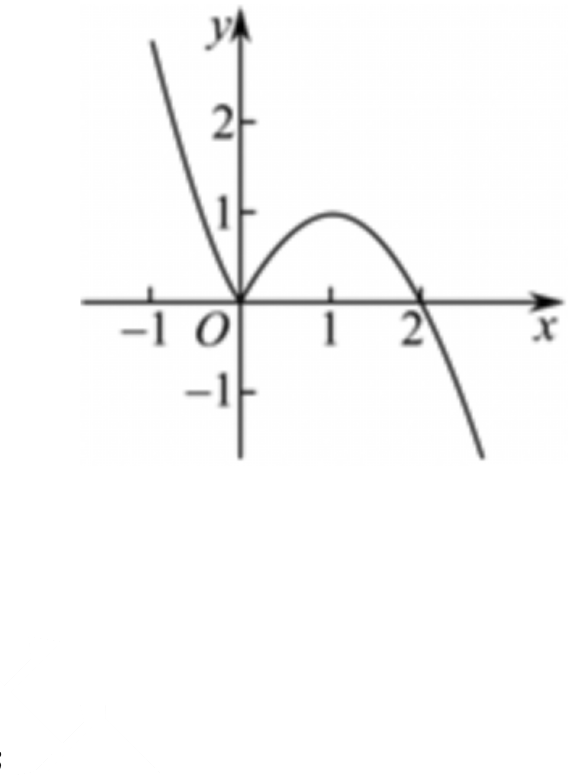
\includegraphics[width=0.20\textwidth]{figures/gao83_q15_graph.png}
\end{center}
\step{由 $[f(x)]^2+af(x)<0$ 得 $[f(x)+a]f(x)<0$，}
\step{当 $a=0$ 时，$[f(x)]^2<0$，不等式无解；}
\step{当 $a>0$ 时，由 $[f(x)+a]f(x)<0$ 得 $-a<f(x)<0$，}
\step{若不等式恰有 $1$ 个整数解，则整数解为 $3$，}
\step{又 $f(3)=-3$，$f(4)=-8$，所以 $-8\leqslant-a<-3$，所以 $3<a\leqslant8$；}
\step{当 $a<0$ 时，由 $[f(x)+a]f(x)<0$ 得 $0<f(x)<-a$，此时有多个解，故舍去；}
\step{综上所述，实数 $a$ 的取值范围为 $(3,8]$. 故选 $C$.}
\solend
\fi

\item 设函数 $f(x)=\begin{cases}\lvert2^x-1\rvert,&x\leqslant2\\ -x+7,&x>2\end{cases}$，若互不相等的实数 $a$、$b$、$c$ 满足 $f(a)=f(b)=f(c)$，
则 $2^a+2^b+2^c$ 的取值范围是\mbox{（\quad）}

\keepwithprev
A. $(8,9)$\qquad B. $(65,129)$\qquad C. $(64,128)$\qquad D. $(66,130)$

\ifanswer
\solbegin
\step{作出函数 $f(x)=\begin{cases}\lvert2^x-1\rvert,&x\leqslant2\\ -x+7,&x>2\end{cases}$ 的图象如图，}
\begin{center}
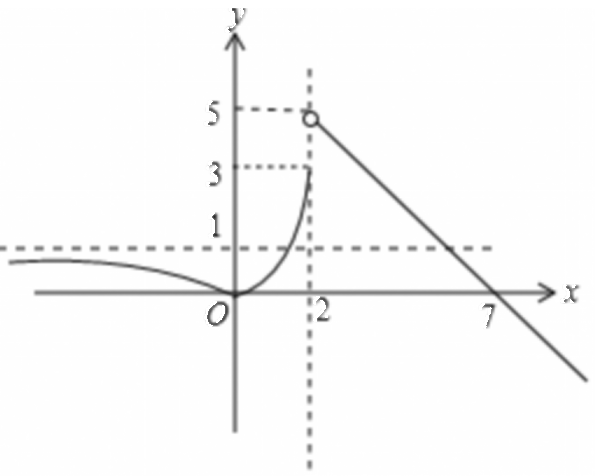
\includegraphics[width=0.22\textwidth]{figures/gao83_q16_graph.png}
\end{center}
\step{不妨设 $a<b<c$，由 $f(a)=f(b)$，得 $1-2^a=2^b-1$，则 $2^a+2^b=2$.}
\step{由 $f(-c)-c+6\in(0,1)$，得 $c\in(6,7)$，则 $64<2^c<128$，}
\step{所以 $66<2^a+2^b+2^c<130$，即 $2^a+2^b+2^c$ 的取值范围是 $(66,130)$. 故选 $D$.}
\solend
\fi

\end{enumerate}

\bigsec{三、解答题}

\begin{enumerate}
\setcounter{enumi}{16}

\item 已知幂函数 $f(x)$ 与一次函数 $g(x)$ 的图象都经过点 $(4,2)$，且 $f(9)=g(5)$.

（1）求 $f(x)$ 与 $g(x)$ 的解析式；

（2）求函数 $h(x)=g(x)-f(x)$ 在 $[0,4]$ 上的值域.

\ansspace*[8]

\ifanswer
\solbegin
\stepm{（1）}{设 $f(x)=x^\alpha$，$g(x)=kx+b$，则 $4^\alpha=2$，即 $\alpha=\dfrac12$，}
\step{$\begin{cases}4k+b=2\\ 3=5k+b\end{cases}$，则 $k=1$，$b=-2$，所以 $f(x)=\sqrt x$，$g(x)=x-2$；}
\stepm{（2）}{$h(x)=g(x)-f(x)=x-\sqrt x-2$，}
\step{令 $t=\sqrt x$，则 $t\in[0,2]$，原函数可化为 $p(t)=t^2-t-2$，}
\step{当 $t=\dfrac12$ 时，函数取得最小值 $-\dfrac94$，当 $t=2$ 时，函数取得最大值 $0$，}
\step{即函数值域为 $\left[-\dfrac94,0\right]$.}
\solend
\fi

\item 目前某县有 $100$ 万人. 经过 $x$ 年后为 $y$ 万人. 如果年平均增长率是 $1.2\%$. 请回答下列问题：

（1）写出 $y$ 关于 $x$ 的函数解析式.

（2）计算 $10$ 年后该县的人口总数（精确到 $0.1$ 万人）.

（3）计算大约多少年后该县的人口总数将达到 $120$ 万（精确到 $1$ 年）.

\ansspace*[9]

\ifanswer
\solbegin
\stepm{（1）}{当 $x=1$ 时，$y=100+100\times1.2\%=100(1+1.2\%)$，}
\step{当 $x=2$ 时，$y=100(1+1.2\%)+100(1+1.2\%)\times1.2\%=100(1+1.2\%)^2$，}
\step{当 $x=3$ 时，$y=100(1+1.2\%)^2+100(1+1.2\%)^2\times1.2\%=100(1+1.2\%)^3$，}
\step{$\cdots\cdots$}
\step{故 $y$ 关于 $x$ 的函数解析式为 $y=100(1+1.2\%)^x\,(x\in\N^*)$；}
\stepm{（2）}{当 $x=10$ 时，$y=100(1+1.2\%)^{10}=100\times1.012^{10}\approx112.7$，}
\step{故 $10$ 年后该县的人口总数约为 $112.7$ 万人；}
\stepm{（3）}{设 $x$ 年后该县的人口总数将达到 $120$ 万，即 $y=100(1+1.2\%)^x=120$，}
\step{解得 $x=\log_{1.012}\dfrac{120}{100}\approx16$，故大约 $16$ 年后该县的人口总数将达到 $120$ 万.}
\solend
\fi

\item 已知 $a>0$ 且 $a\neq1$，$m>0$，函数 $f(x)=(m^2+m-5)a^x$ 是指数函数，且 $f(2)=4$.

（1）求实数 $m$ 和 $a$ 的值；

（2）$f(2x)-2f(x)+2\geqslant nf(x)$ 对任意 $x\in[-1,2]$ 恒成立，求实数 $n$ 的取值范围；

（3）若关于 $x$ 的方程 $f(2x)-(2k+8)f(x)+2k+7b=0$ 有两个不相等的实数根，且一根
大于 $0$，另一根小于 $0$，其中 $k>0$，求整数 $b$ 的最大值.

\ansspace*[11]

\ifanswer
\solbegin
\stepm{（1）}{因为函数 $f(x)=(m^2+m-5)a^x$ 是指数函数，}
\step{所以 $m^2+m-5=1$，即 $m^2+m-6=0$，解得 $m=2$ 或 $m=-3$，}
\step{又 $m>0$，所以 $m=2$，又 $f(2)=a^2=4$，$a>0$ 且 $a\neq1$，所以 $a=2$；}
\stepm{（2）}{由（1）得 $f(x)=2^x$，}
\step{由题意 $2^{2x}-2\cdot2^x+2\geqslant n2^x$ 对任意 $x\in[-1,2]$ 恒成立，}
\step{所以 $n\leqslant2^x-2+\dfrac2{2^x}$ 对任意 $x\in[-1,2]$ 恒成立，则 $n\leqslant\left(2^x-2+\dfrac2{2^x}\right)_{\min}$，}
\step{记 $g(x)=2^x-2+\dfrac2{2^x}$，$x\in[-1,2]$，}
\step{令 $t=2^x$，因为 $x\in[-1,2]$，所以 $t\in\left[\dfrac12,4\right]$，则 $y=t+\dfrac2t-2$，$t\in\left[\dfrac12,4\right]$，}
\step{函数 $y=t+\dfrac2t-2$ 在 $\left[\dfrac12,\sqrt2\right]$ 上严格减，在 $[\sqrt2,4]$ 上严格增，}
\step{所以 $y=t+\dfrac2t-2$ 的最小值为 $\sqrt2+\dfrac2{\sqrt2}-2=2\sqrt2-2$，}
\step{所以 $n\leqslant2\sqrt2-2$，即实数 $n$ 的取值范围为 $(-\infty,2\sqrt2-2]$；}
\stepm{（3）}{方程 $f(2x)-(2k+8)f(x)+2k+7b=0$，}
\step{即方程 $2^{2x}-(2k+8)2^x+2k+7b=0$，即方程 $(2^x)^2-(2k+8)2^x+2k+7b=0$，}
\step{令 $t=2^x>0$，则方程 $t^2-(2k+8)t+2k+7b=0$，}
\step{因为关于 $x$ 的方程 $f(2x)-(2k+8)f(x)+2k+7b=0$ 的一根大于 $0$，另一根小于 $0$，}
\step{所以关于 $t$ 的方程 $t^2-(2k+8)t+2k+7b=0$ 的一根大于 $1$，另一根大于 $0$ 且小于 $1$，}
\step{记 $h(t)=t^2-(2k+8)t+2k+7b$，}
\step{所以 $\begin{cases}h(1)=1^2-(2k+8)\cdot1+2k+7b<0\\ h(0)=2k+7b>0\\ k>0\end{cases}$，所以 $\begin{cases}b<1\\ b>-\dfrac27k\\ k>0\end{cases}$，}
\step{所以整数 $b$ 的最大值为 $0$.}
\solend
\fi

\item 已知幂函数 $f(x)=(p^2-3p+3)x^{p^2-\frac32p-\frac12}$ 满足 $f(2)<f(4)$.

（1）求函数 $f(x)$ 的解析式；

（2）若函数 $g(x)=f^2(x)+mf(x)$，$x\in[1,9]$，是否存在实数 $m$ 使得 $g(x)$ 的最小值为 $0$？
若存在，求出 $m$ 的值；若不存在，说明理由.

（3）若函数 $h(x)=n-f(x+3)$，是否存在实数 $a$、$b\,(a<b)$，使函数 $h(x)$ 在 $[a,b]$ 上的
值域为 $[a,b]$？若存在，求出实数 $n$ 的取值范围；若不存在，说明理由.

\ansspace*[12]

\ifanswer
\solbegin
\stepm{（1）}{因为 $f(x)$ 是幂函数，所以 $p^2-3p+3=1$，解得 $p=1$ 或 $p=2$，}
\step{当 $p=1$ 时，$f(x)=\dfrac1x$，不满足 $f(2)<f(4)$.}
\step{当 $p=2$ 时，$f(x)=\sqrt x$，满足 $f(2)<f(4)$.}
\step{故 $p=2$，函数 $f(x)$ 的解析式为 $f(x)=\sqrt x$；}
\stepm{（2）}{由函数 $g(x)=f^2(x)+mf(x)$，即 $g(x)=(\sqrt x)^2+m\sqrt x$，}
\step{令 $t=\sqrt x$，因为 $x\in[1,9]$，所以 $t\in[1,3]$，}
\step{记 $k(x)=t^2+mt$，其对称轴 $t=-\dfrac m2$，}
\step{①当 $-\dfrac m2\leqslant1$，即 $m\geqslant-2$ 时，则 $k(x)_{\min}=k(1)=1+m=0$，解得 $m=-1$；}
\step{②当 $1<-\dfrac m2<3$ 时，即 $-6<m<-2$，则 $k(x)_{\min}=k\left(-\dfrac m2\right)=-\dfrac{m^2}4=0$，}
\step{解得 $m=0$，不满足，舍去；}
\step{③当 $-\dfrac m2\geqslant3$ 时，即 $m\leqslant-6$ 时，则 $k(x)_{\min}=k(3)=3m+9=0$，解得 $m=-3$，}
\step{不满足，舍去；}
\step{综上所述，存在 $m=-1$ 使得 $g(x)$ 的最小值为 $0$；}
\stepm{（3）}{由函数 $h(x)=n-f(x+3)=n-\sqrt{x+3}$ 在定义域内为严格减函数，}
\step{若存在实数 $a$、$b\,(a<b)$，使函数 $h(x)$ 在 $[a,b]$ 上的值域为 $[a,b]$，}
\step{则 $h(x)=\begin{cases}n-\sqrt{a+3}=b\text{ ①}\\ n-\sqrt{b+3}=a\text{ ②}\end{cases}$，}
\step{两式相减得 $\sqrt{a+3}-\sqrt{b+3}=a-b=(a+3)-(b+3)$，}
\step{所以 $\sqrt{a+3}+\sqrt{b+3}=1$ ③，}
\step{将③代入②得 $n=a+\sqrt{b+3}=a+1-\sqrt{a+3}$，}
\step{令 $t=\sqrt{a+3}$，因为 $a<b$，所以 $0\leqslant t<\dfrac12$，得 $n=t^2-t-2=\left(t-\dfrac12\right)^2-\dfrac94$，}
\step{故实数 $n$ 的取值范围为 $\left(-\dfrac94,-2\right]$.}
\solend
\fi

\item 定理（三角不等式），对于任意的 $a$、$b\in\R$，恒有 $\bigl\lvert\lvert a\rvert-\lvert b\rvert\bigr\rvert\leqslant\lvert a\pm b\rvert\leqslant\lvert a\rvert+\lvert b\rvert$. 定义：
已知 $n\in\N$ 且 $n\geqslant3$，对于有序数组 $a_1$、$a_2$、$\cdots$、$a_n$，称 $\lvert a_1-a_2\rvert+\lvert a_2-a_3\rvert+\cdots+\lvert a_{n-1}-a_n\rvert$
为有序数组 $a_1$、$a_2$、$\cdots$、$a_n$ 的波动距离，记作 $f(a_1,a_2,\cdots,a_n)$，即
$f(a_1,a_2,\cdots,a_n)=\lvert a_1-a_2\rvert+\lvert a_2-a_3\rvert+\cdots+\lvert a_{n-1}-a_n\rvert$，请根据上述信息解决以下几个问题：

（1）求函数 $y=\lvert x-2\rvert+\lvert x-4\rvert$ 的最小值，并指出函数取到最小值时 $x$ 的取值范围；

（2）①求有序数组 $2$、$5$、$3$、$4$ 的波动距离 $f(2,5,3,4)$；

②求证：若 $a$、$b$、$c$、$d\in\R$ 且 $a<b<c$，则 $f(a,b,c,d)\leqslant f(a,c,b,d)$；

（3）同理可证得命题“若 $a$、$b$、$c$、$d\in\R$ 且 $c<b<a$ 时，$f(a,b,c,d)\leqslant f(a,c,b,d)$”也
是真命题（注：该命题无需证明，需要时可直接使用）.

设两两不相等的四个实数 $a_1$、$a_2$、$a_3$、$a_4\in\{3^1,3^2,3^3,3^4\}$，求有序数组 $a_1$、$a_2$、$a_3$、$a_4$ 的
波动距离 $f(a_1,a_2,a_3,a_4)$ 的最大值.

\ansspace*[14]

\ifanswer
\solbegin
\stepm{（1）}{由三角不等式得 $\bigl\lvert\lvert a\rvert-\lvert b\rvert\bigr\rvert\leqslant\lvert a\pm b\rvert\leqslant\lvert a\rvert+\lvert b\rvert$，}
\step{当且仅当 $\lvert a+b\rvert^2=(\lvert a\rvert+\lvert b\rvert)^2$ 时，}
\step{即当 $-ab=\lvert ab\rvert$ 时，即当 $ab\leqslant0$ 时取等号，}
\step{由三角不等式得 $y=\lvert x-2\rvert+\lvert x-4\rvert\geqslant\lvert(x-2)-(x-4)\rvert=2$，}
\step{当且仅当 $(x-2)(x-4)\leqslant0$ 时，即 $2\leqslant x\leqslant4$ 时取等号，}
\step{因此，函数 $y=\lvert x-2\rvert+\lvert x-4\rvert$ 的最小值为 $2$，此时 $x$ 的取值范围是 $[2,4]$.}
\stepm{（2）}{①由题中定义得 $f(2,5,3,4)=\lvert2-5\rvert+\lvert5-3\rvert+\lvert3-4\rvert=6$；}
\step{②$f(a,b,c,d)-f(a,c,b,d)=\lvert a-b\rvert+\lvert c-d\rvert-\lvert a-c\rvert-\lvert b-d\rvert$，}
\step{因为 $a<b<c$，所以 $\lvert a-b\rvert-\lvert a-c\rvert=-\lvert b-c\rvert$，$\lvert c-d\rvert-\lvert b-d\rvert\leqslant\lvert b-c\rvert$，}
\step{所以 $f(a,b,c,d)-f(a,c,b,d)\leqslant0$，即 $f(a,b,c,d)\leqslant f(a,c,b,d)$，}
\stepm{（3）}{$f(a,b,c,d)=\lvert a-b\rvert+\lvert b-c\rvert+\lvert c-d\rvert$}
\step{$=\lvert d-c\rvert+\lvert c-b\rvert+\lvert b-a\rvert=f(d,c,b,a)$，}
\step{当 $f(a_1,a_2,a_3,a_4)$ 取得最大值时，$a_2=\max\{a_1,a_2,a_3\}$ 或 $a_2=\min\{a_1,a_2,a_3\}$，}
\step{同理 $a_3=\max\{a_2,a_3,a_4\}$ 或 $a_3=\min\{a_2,a_3,a_4\}$，}
\step{若 $a_2=\max\{a_1,a_2,a_3\}$，则 $a_2>a_3$，所以 $a_3=\min\{a_2,a_3,a_4\}$，}
\step{故 $f(a_1,a_2,a_3,a_4)=\lvert a_1-a_2\rvert+\lvert a_2-a_3\rvert+\lvert a_3-a_4\rvert=a_2-a_1+a_2-a_3+a_4-a_3$}
\step{$=2a_2+a_4-2a_3-a_1\leqslant2\times3^4+3^3-2\times3^1-3^2=174$，}
\step{当且仅当 $a_1=3^2$，$a_2=3^4$，$a_3=3^1$，$a_4=3^3$ 时取等号，}
\step{所以 $f(3^2,3^4,3^1,3^3)$ 为 $f(a_1,a_2,a_3,a_4)$ 的最大值，}
\step{若 $a_2=\min\{a_1,a_2,a_3\}$，则 $a_2<a_3$，所以 $a_3=\max\{a_2,a_3,a_4\}$，}
\step{同理可得 $f(3^3,3^4,3^1,3^2)$ 为 $f(a_1,a_2,a_3,a_4)$ 的最大值，}
\step{综上所述，$f(a_1,a_2,a_3,a_4)$ 的最大值为 $174$.}
\solend
\fi

\end{enumerate}

\end{document}
"
%
% 原始材料：微信公众号“魔都数学加油站”文章，连载“27学年高一83”；
% 原文标题“27学年高一83——2026-2027年上海市交附闵行高一上周末作业10.23”；
% 原文链接：https://mp.weixin.qq.com/s/t5AfTwQXg4Sj4i_Dl5rgXA。
% 页面标注发布时间 2026-10-26 20:15（上海）。
% 正文为 12 张 PNG 页（`原图/高一83_交附闵行_周末作业10.23/01..12.png`），
% 尺寸混排（第 1—8 页为 4762×6735，第 9—12 页为 2560×3620），均按页序读取。
%
% 篇幅与题号：原卷自第 3 题起编号（第 1、2 题不在原文内）。填空题 3—12（10 题）、
% 选择题 13—16（4 题）、解答题 17—21（5 题），共 19 题。
%
% 讲评版：19 题全部印【解析】，本稿不另提 \ans{}；选择题答案在解析末句“故选 C／B／C／D”。
%
% 副标题：原卷未印副标题。本稿按内容标作“函数与导数”（本卷考幂函数、指数函数、
% 对数与函数应用，属“函数与导数”模块；副标题只用知识模块名，见 README 说明）。
%
% 与原卷的排版差异：
%   ① 原卷每题下直接印【解析】，本稿按全稿惯例将解析置于答案版；
%   ② 原卷未印副标题，本稿补出；填空横线统一排 \blankline[4.4em]；
%   ③ 原卷数集记号排斜体 $R$、$Z$、$N$，本稿按全稿惯例改用 $\R$、$\Z$、$\N$；
%   ④ 第 17—21 题的子问用行内“（1）（2）（3）”段，解析中的子问标号用 \stepm；
%   ⑤ 解答题按惯例加 \ansspace；选择题括号排 \mbox{（\quad）}；
%   ⑥ 第 15、16 题解析各有一幅函数图象，裁自原图（第 6 页）后去粉色水印、转灰度，
%      仅答案版出。
%
% 行数核对：逐题数 \step/\stepm 条数，合计 145 条（Q3：1；Q4：1；Q5：4；Q6：5；
% Q7：2；Q8：7；Q9：10；Q10：5；Q11：6；Q12：8；Q13：3；Q14：4；Q15：8；
% Q16：4；Q17：6；Q18：9；Q19：19；Q20：21；Q21：22）。原卷解析的换行
% 按语意合并，未逐行强拆。
%
\documentclass[a4paper,11pt]{article}
\usepackage{common}

\begin{document}

\examtitlest[4]{2026--2027 年交附闵行高一上周末作业 10.23}{函数与导数}

\bigsec{一、填空题}

\begin{enumerate}
\setcounter{enumi}{2}

\item 已知 $10^a=2$，$10^b=5$，则 $10^{3a-2b}$ 的值为\blankline[4.4em].

\ifanswer
\solbegin
\step{$10^{3a-2b}=\dfrac{10^{3a}}{10^{2b}}=\dfrac{(10^a)^3}{(10^b)^2}=\dfrac{2^3}{5^2}=\dfrac8{25}$.}
\solend
\fi

\item 根式 $a\sqrt{-a}$ 化成分数指数幂是\blankline[4.4em].

\ifanswer
\solbegin
\step{$a\sqrt{-a}=a(-a)^{\frac12}=-(-a)(-a)^{\frac12}=-(-a)^{\frac32}$.}
\solend
\fi

\item 已知数列 $\{a_n\}$ 的通项公式为 $a_n=\left(\dfrac49\right)^{n-1}-\left(\dfrac23\right)^{n-1}$，在下列说法中：①有最大项；
②有最小项；③没有最大项；④没有最小项. 正确的是\blankline[3.6em]（填序号）.

\ifanswer
\solbegin
\step{令 $t=\left(\dfrac23\right)^{n-1}$，则 $t\in\left\{1,\dfrac23,\dfrac49,\dfrac8{27},\cdots\right\}\subset(0,1]$，$t$ 是关于 $n$ 的减函数，}
\step{则 $a_n=t^2-t=\left(t-\dfrac12\right)^2-\dfrac14$，}
\step{所以当 $t=1$ 即 $n=1$ 时 $a_n$ 取得最大为 $0$，当 $t=\dfrac49$ 即 $n=3$ 时 $a_n$ 取得最小为 $-\dfrac{20}{81}$，}
\step{所以 $a_n$ 既有最大项又有最小项，故①和②正确.}
\solend
\fi

\item 已知 $f(x)=\mathrm{e}^{x-\frac12}-\mathrm{e}^{-x+\frac12}+\dfrac{4x}{2x-1}$，则
$f\left(\dfrac1{2020}\right)+f\left(\dfrac2{2020}\right)+f\left(\dfrac3{2020}\right)+\cdots+f\left(\dfrac{1009}{2020}\right)+f\left(\dfrac{1011}{2020}\right)+\cdots+f\left(\dfrac{2019}{2020}\right)$ 的
值为\blankline[4.4em].

\ifanswer
\solbegin
\step{因为 $f(x)+f(1-x)=\mathrm{e}^{x-\frac12}-\mathrm{e}^{-x+\frac12}+\dfrac{4x}{2x-1}+\mathrm{e}^{(1-x)-\frac12}-\mathrm{e}^{-(1-x)+\frac12}+\dfrac{4(1-x)}{2(1-x)-1}$}
\step{$=\dfrac{4x}{2x-1}+\dfrac{4-4x}{1-2x}=\dfrac{4(2x-1)}{2x-1}=4$，}
\step{记 $S=f\left(\dfrac1{2020}\right)+f\left(\dfrac2{2020}\right)+\cdots+f\left(\dfrac{2019}{2020}\right)$，}
\step{又 $S=f\left(\dfrac{2019}{2020}\right)+f\left(\dfrac{2018}{2020}\right)+\cdots+f\left(\dfrac2{2020}\right)+f\left(\dfrac1{2020}\right)$，}
\step{对齐相加得 $2S=2018\times4$，所以 $S=4036$.}
\solend
\fi

\item 不等式 $2^{x^2-2x-3}<\left(\dfrac12\right)^{3(x-1)}$ 的解集为\blankline[4.4em].

\ifanswer
\solbegin
\step{由 $2^{x^2-2x-3}<\left(\dfrac12\right)^{3(x-1)}$ 得 $x^2-2x-3<-3(x-1)$，即 $x^2+x-6<0$，}
\step{故解集为 $(-3,2)$.}
\solend
\fi

\item 函数 $f(x)=x^{\ln5}+x^{\ln12}-13^{\ln x}$ 的零点是\blankline[4.4em]. 附：$a^{\log_bc}=c^{\log_ba}$
（$a>0$，$b>0$，$c>0$，$b\neq1$）.

\ifanswer
\solbegin
\step{函数 $f(x)=x^{\ln5}+x^{\ln12}-13^{\ln x}$，}
\step{若 $f(x)=x^{\ln5}+x^{\ln12}-13^{\ln x}=0$，变形得 $x^{\ln5}+x^{\ln12}=13^{\ln x}$，}
\step{又 $a^{\log_bc}=c^{\log_ba}$（$a>0$，$b>0$，$c>0$，$b\neq1$），得 $5^{\ln x}+12^{\ln x}=13^{\ln x}$，}
\step{令 $g(t)=\left(\dfrac5{13}\right)^t+\left(\dfrac{12}{13}\right)^t-1$，易得 $g(t)$ 严格减，所以 $g(t)=0$ 至多有一解，}
\step{即 $\left(\dfrac5{13}\right)^t+\left(\dfrac{12}{13}\right)^t-1=0$ 至多有一解，变形得方程 $5^t+12^t=13^t$ 至多有一解，}
\step{易得 $t=2$ 时，有 $5^2+12^2=13^2$ 成立，则方程 $5^t+12^t=13^t$ 有唯一解 $t=2$，}
\step{即 $\ln x=2$，解得 $x=\mathrm{e}^2$，即函数 $f(x)$ 的零点为 $\mathrm{e}^2$.}
\solend
\fi

\item 已知幂函数 $f(x)=(m^2-2m-2)x^{m^2+m-2}$ 在 $(0,+\infty)$ 上是严格减函数，则不等式
$f(x-1)<f(3-2x)$ 的解集为\blankline[4.4em].

\ifanswer
\solbegin
\step{因为 $f(x)$ 为幂函数，所以 $m^2-2m-2=1$，解得 $m=-1$ 或 $m=3$；}
\step{当 $m=3$ 时，$f(x)=x^{10}$ 在 $(0,+\infty)$ 上严格增，不合题意；}
\step{当 $m=-1$ 时，$f(x)=x^{-2}$ 在 $(0,+\infty)$ 上严格减，符合题意；}
\step{综上所述，$m=-1$；}
\step{因为 $f(x)=x^{-2}$ 的定义域为 $(-\infty,0)\cup(0,+\infty)$，$f(-x)=(-x)^{-2}=x^{-2}=f(x)$，}
\step{所以 $f(x)$ 为定义在 $(-\infty,0)\cup(0,+\infty)$ 上的偶函数，}
\step{故 $f(x-1)=f(\lvert x-1\rvert)$，$f(3-2x)=f(\lvert3-2x\rvert)$，}
\step{$f(x-1)<f(3-2x)\Rightarrow f(\lvert x-1\rvert)<f(\lvert3-2x\rvert)\Rightarrow\lvert x-1\rvert>\lvert3-2x\rvert$}
\step{且 $\lvert x-1\rvert\neq0$，$\lvert3-2x\rvert\neq0$，解得 $\dfrac43<x<\dfrac32$ 或 $\dfrac32<x<2$，}
\step{所以 $f(x-1)<f(3-2x)$ 的解集为 $\left(\dfrac43,\dfrac32\right)\cup\left(\dfrac32,2\right)$.}
\solend
\fi

\item 若实数 $x_1$、$x_2$ 满足 $\mathrm{e}^{x_1}+x_1-3=0$，$x_2\ln x_2+3x_2-1=0$，则 $\dfrac{x_1x_2+1}{x_2}$ 的值为\blankline[4.4em].

\ifanswer
\solbegin
\step{易得 $x_2>0$，则 $\ln x_2+3-\dfrac1{x_2}=0$，即 $\mathrm{e}^{-\ln x_2}+(-\ln x_2)-3=0$.}
\step{设 $f(x)=\mathrm{e}^x+x-3$，则函数 $f(x)$ 在 $(-\infty,+\infty)$ 上严格增.}
\step{由 $\mathrm{e}^{x_1}+x_1-3=0$，$\mathrm{e}^{-\ln x_2}+(-\ln x_2)-3=0$，得 $f(x_1)=0$，$f(-\ln x_2)=0$，}
\step{所以 $f(x_1)=f(-\ln x_2)$，得 $x_1=-\ln x_2$，即 $\ln x_2=-x_1$，所以 $x_2=\mathrm{e}^{-x_1}$，得 $\dfrac1{x_2}=\mathrm{e}^{x_1}$.}
\step{因为 $\mathrm{e}^{x_1}+x_1-3=0$，所以 $\mathrm{e}^{x_1}+x_1=3$，所以 $\dfrac{x_1x_2+1}{x_2}=x_1+\dfrac1{x_2}=\mathrm{e}^{x_1}+x_1=3$.}
\solend
\fi

\item 已知 $\alpha$、$\beta$ 是方程 $9^x-2m\cdot3^x+m^2-1=0$ 的两个根，若 $\alpha+\beta=1$，则 $\alpha\beta=\blankline[4.4em]$.

\ifanswer
\solbegin
\step{由题意得方程 $9^x-2m\cdot3^x+m^2-1=0$ 有两个根，}
\step{则方程 $t^2-2mt+m^2-1=0$ 有二正根，则 $\begin{cases}\Delta=4m^2-4(m^2-1)\geqslant0\\ 2m>0\\ m^2-1>0\end{cases}$，解得 $m>1$，}
\step{又 $\alpha$、$\beta$ 是方程 $9^x-2m\cdot3^x+m^2-1=0$ 的两个根，则 $3^\alpha\times3^\beta=m^2-1$，}
\step{又 $\alpha+\beta=1$，则 $m^2-1=3^{\alpha+\beta}=3$，解得 $m=2$ 或 $m=-2$（舍），}
\step{则 $3^\alpha+3^\beta=2m=4$，又 $\alpha=1-\beta$，则 $3^{1-\beta}+3^\beta=4$，解得 $\beta=0$ 或 $\beta=1$，}
\step{则 $\begin{cases}\alpha=1\\ \beta=0\end{cases}$ 或 $\begin{cases}\alpha=0\\ \beta=1\end{cases}$，则 $\alpha\beta=0$.}
\solend
\fi

\item 已知实数 $a,b,c\in(1,+\infty)$，满足 $a^{\log_ba}\cdot b^{\log_cb}\cdot c^{\log_ac}=100$，则 $abc$ 的最大值为\blankline[4.4em].

\ifanswer
\solbegin
\step{由换底公式得 $\log_ba=\dfrac{\ln a}{\ln b}$，$\log_cb=\dfrac{\ln b}{\ln c}$，$\log_ac=\dfrac{\ln c}{\ln a}$，}
\step{设 $X=\ln a$，$Y=\ln b$，$Z=\ln c$，得 $a=\mathrm{e}^X$，$b=\mathrm{e}^Y$，$c=\mathrm{e}^Z$，}
\step{代入得 $a^{\log_ba}\cdot b^{\log_cb}\cdot c^{\log_ac}=a^{\frac{\ln a}{\ln b}}\cdot b^{\frac{\ln b}{\ln c}}\cdot c^{\frac{\ln c}{\ln a}}=(\mathrm{e}^X)^{\frac XY}\cdot(\mathrm{e}^Y)^{\frac YZ}\cdot(\mathrm{e}^Z)^{\frac ZX}=100$，}
\step{即 $\mathrm{e}^{\frac{X^2}Y+\frac{Y^2}Z+\frac{Z^2}X}=100$，两边取对数得 $\dfrac{X^2}Y+\dfrac{Y^2}Z+\dfrac{Z^2}X=\ln100$.}
\step{由 $a,b,c\in(1,+\infty)$，得 $X>0$，$Y>0$，$Z>0$，}
\step{由柯西不等式，得 $\left(\dfrac{X^2}Y+\dfrac{Y^2}Z+\dfrac{Z^2}X\right)(X+Y+Z)\geqslant(X+Y+Z)^2$，}
\step{即 $X+Y+Z\leqslant\dfrac{X^2}Y+\dfrac{Y^2}Z+\dfrac{Z^2}X=\ln100$，当且仅当 $X=Y=Z$ 时取等号，}
\step{因此 $(X+Y+Z)_{\max}=\ln100$，所以 $(abc)_{\max}=\mathrm{e}^{(X+Y+Z)_{\max}}=\mathrm{e}^{\ln100}=100$.}
\solend
\fi

\end{enumerate}

\bigsec{二、选择题}

\begin{enumerate}
\setcounter{enumi}{12}

\item 已知集合 $A=\{x\mid x=2k,k\in\Z\}$，$B=\{x\mid x=4k+2,\,k\in\Z\}$，则 $A\cup B=\mbox{（\quad）}$

\keepwithprev
A. $B$\qquad B. $\R$\qquad C. $A$\qquad D. 以上都不是

\ifanswer
\solbegin
\step{$B=\{x\mid x=4k+2,k\in\Z\}=\{x\mid x=2(2k+1),k\in\Z\}$，它表示奇数的 $2$ 倍组成的集合，}
\step{$A=\{x\mid x=2k,k\in\Z\}$，即集合 $A$ 是整数的 $2$ 倍组成的集合，}
\step{则 $B\subseteq A$，则 $A\cup B=A$. 故选 $C$.}
\solend
\fi

\item 教室通风的目的是通过空气的流动，排出室内的污浊空气和致病微生物，降低室内二氧化碳和致病微生物的浓度，送进室外的新鲜空气. 按照国家标准，教室内空气中二氧化碳日平均最高容许浓度应小于等于 $0.1\%$. 经测定，刚下课时，空气中含有 $0.2\%$ 的二氧化碳，若开窗通风后教室内二氧化碳的浓度为 $y\%$，且 $y$ 随时间 $t$（单位：分钟）的变化规律可以用函数 $y=0.05+\lambda\mathrm{e}^{-\frac t{12}}\,(\lambda\in\R)$ 描述，则该教室内的二氧化碳浓度达到国家标准至少需要的时间为\mbox{（\quad）}

\keepwithprev
A. $10$ 分钟\qquad B. $14$ 分钟\qquad C. $15$ 分钟\qquad D. $20$ 分钟

\ifanswer
\solbegin
\step{由题意得，当 $t=0$ 时，$y=0.2$，即 $0.05+\lambda\mathrm{e}^0=0.2$，解得 $\lambda=0.15$，}
\step{所以 $y=0.05+0.15\mathrm{e}^{-\frac t{12}}$，由题意得 $0.05+0.15\mathrm{e}^{-\frac t{12}}\leqslant0.1$，即 $\mathrm{e}^{-\frac t{12}}\leqslant\dfrac13$，}
\step{两边取对数得 $-\dfrac t{12}\leqslant-\ln3$，所以 $t\geqslant12\ln3\approx13.2$，}
\step{所以该教室内的二氧化碳浓度达到国家标准至少需要的时间为 $14$ 分钟. 故选 $B$.}
\solend
\fi

\item 已知函数 $f(x)=\begin{cases}-x^2+2x,&x\geqslant0\\ x^2-2x,&x<0\end{cases}$，若关于 $x$ 的不等式 $[f(x)]^2+af(x)<0$ 恰有 $1$ 个整数
解，则实数 $a$ 的最大值为\mbox{（\quad）}

\keepwithprev
A. $-2$\qquad B. $3$\qquad C. $8$\qquad D. $9$

\ifanswer
\solbegin
\step{作出 $f(x)$ 的图象，如图所示：}
\begin{center}
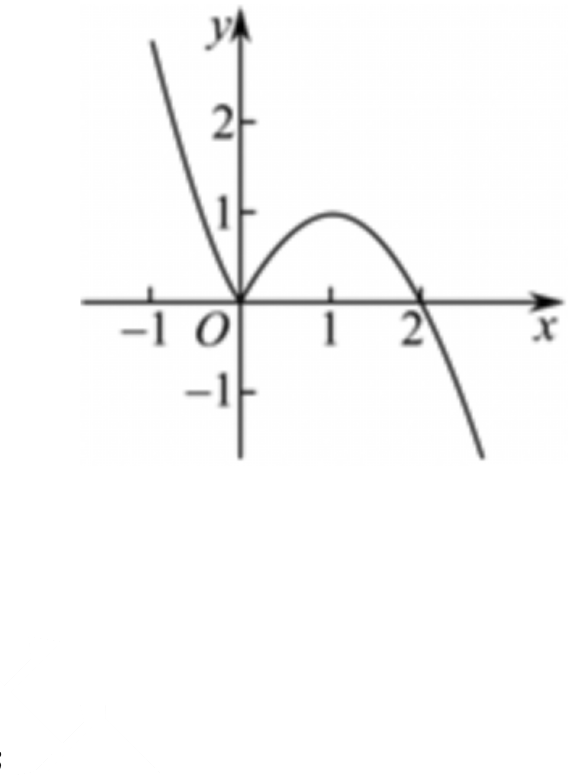
\includegraphics[width=0.20\textwidth]{figures/gao83_q15_graph.png}
\end{center}
\step{由 $[f(x)]^2+af(x)<0$ 得 $[f(x)+a]f(x)<0$，}
\step{当 $a=0$ 时，$[f(x)]^2<0$，不等式无解；}
\step{当 $a>0$ 时，由 $[f(x)+a]f(x)<0$ 得 $-a<f(x)<0$，}
\step{若不等式恰有 $1$ 个整数解，则整数解为 $3$，}
\step{又 $f(3)=-3$，$f(4)=-8$，所以 $-8\leqslant-a<-3$，所以 $3<a\leqslant8$；}
\step{当 $a<0$ 时，由 $[f(x)+a]f(x)<0$ 得 $0<f(x)<-a$，此时有多个解，故舍去；}
\step{综上所述，实数 $a$ 的取值范围为 $(3,8]$. 故选 $C$.}
\solend
\fi

\item 设函数 $f(x)=\begin{cases}\lvert2^x-1\rvert,&x\leqslant2\\ -x+7,&x>2\end{cases}$，若互不相等的实数 $a$、$b$、$c$ 满足 $f(a)=f(b)=f(c)$，
则 $2^a+2^b+2^c$ 的取值范围是\mbox{（\quad）}

\keepwithprev
A. $(8,9)$\qquad B. $(65,129)$\qquad C. $(64,128)$\qquad D. $(66,130)$

\ifanswer
\solbegin
\step{作出函数 $f(x)=\begin{cases}\lvert2^x-1\rvert,&x\leqslant2\\ -x+7,&x>2\end{cases}$ 的图象如图，}
\begin{center}
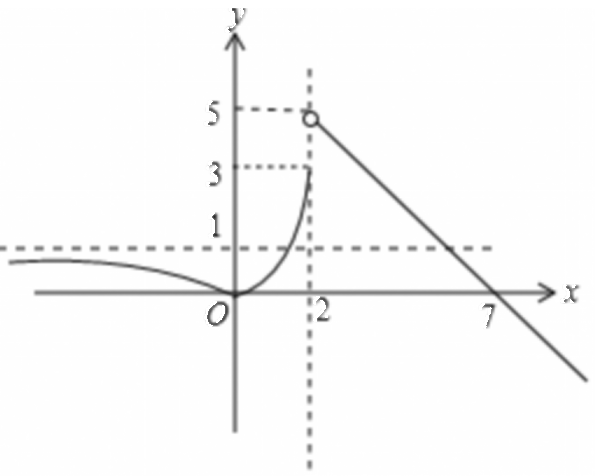
\includegraphics[width=0.22\textwidth]{figures/gao83_q16_graph.png}
\end{center}
\step{不妨设 $a<b<c$，由 $f(a)=f(b)$，得 $1-2^a=2^b-1$，则 $2^a+2^b=2$.}
\step{由 $f(-c)-c+6\in(0,1)$，得 $c\in(6,7)$，则 $64<2^c<128$，}
\step{所以 $66<2^a+2^b+2^c<130$，即 $2^a+2^b+2^c$ 的取值范围是 $(66,130)$. 故选 $D$.}
\solend
\fi

\end{enumerate}

\bigsec{三、解答题}

\begin{enumerate}
\setcounter{enumi}{16}

\item 已知幂函数 $f(x)$ 与一次函数 $g(x)$ 的图象都经过点 $(4,2)$，且 $f(9)=g(5)$.

（1）求 $f(x)$ 与 $g(x)$ 的解析式；

（2）求函数 $h(x)=g(x)-f(x)$ 在 $[0,4]$ 上的值域.

\ansspace*[8]

\ifanswer
\solbegin
\stepm{（1）}{设 $f(x)=x^\alpha$，$g(x)=kx+b$，则 $4^\alpha=2$，即 $\alpha=\dfrac12$，}
\step{$\begin{cases}4k+b=2\\ 3=5k+b\end{cases}$，则 $k=1$，$b=-2$，所以 $f(x)=\sqrt x$，$g(x)=x-2$；}
\stepm{（2）}{$h(x)=g(x)-f(x)=x-\sqrt x-2$，}
\step{令 $t=\sqrt x$，则 $t\in[0,2]$，原函数可化为 $p(t)=t^2-t-2$，}
\step{当 $t=\dfrac12$ 时，函数取得最小值 $-\dfrac94$，当 $t=2$ 时，函数取得最大值 $0$，}
\step{即函数值域为 $\left[-\dfrac94,0\right]$.}
\solend
\fi

\item 目前某县有 $100$ 万人. 经过 $x$ 年后为 $y$ 万人. 如果年平均增长率是 $1.2\%$. 请回答下列问题：

（1）写出 $y$ 关于 $x$ 的函数解析式.

（2）计算 $10$ 年后该县的人口总数（精确到 $0.1$ 万人）.

（3）计算大约多少年后该县的人口总数将达到 $120$ 万（精确到 $1$ 年）.

\ansspace*[9]

\ifanswer
\solbegin
\stepm{（1）}{当 $x=1$ 时，$y=100+100\times1.2\%=100(1+1.2\%)$，}
\step{当 $x=2$ 时，$y=100(1+1.2\%)+100(1+1.2\%)\times1.2\%=100(1+1.2\%)^2$，}
\step{当 $x=3$ 时，$y=100(1+1.2\%)^2+100(1+1.2\%)^2\times1.2\%=100(1+1.2\%)^3$，}
\step{$\cdots\cdots$}
\step{故 $y$ 关于 $x$ 的函数解析式为 $y=100(1+1.2\%)^x\,(x\in\N^*)$；}
\stepm{（2）}{当 $x=10$ 时，$y=100(1+1.2\%)^{10}=100\times1.012^{10}\approx112.7$，}
\step{故 $10$ 年后该县的人口总数约为 $112.7$ 万人；}
\stepm{（3）}{设 $x$ 年后该县的人口总数将达到 $120$ 万，即 $y=100(1+1.2\%)^x=120$，}
\step{解得 $x=\log_{1.012}\dfrac{120}{100}\approx16$，故大约 $16$ 年后该县的人口总数将达到 $120$ 万.}
\solend
\fi

\item 已知 $a>0$ 且 $a\neq1$，$m>0$，函数 $f(x)=(m^2+m-5)a^x$ 是指数函数，且 $f(2)=4$.

（1）求实数 $m$ 和 $a$ 的值；

（2）$f(2x)-2f(x)+2\geqslant nf(x)$ 对任意 $x\in[-1,2]$ 恒成立，求实数 $n$ 的取值范围；

（3）若关于 $x$ 的方程 $f(2x)-(2k+8)f(x)+2k+7b=0$ 有两个不相等的实数根，且一根
大于 $0$，另一根小于 $0$，其中 $k>0$，求整数 $b$ 的最大值.

\ansspace*[11]

\ifanswer
\solbegin
\stepm{（1）}{因为函数 $f(x)=(m^2+m-5)a^x$ 是指数函数，}
\step{所以 $m^2+m-5=1$，即 $m^2+m-6=0$，解得 $m=2$ 或 $m=-3$，}
\step{又 $m>0$，所以 $m=2$，又 $f(2)=a^2=4$，$a>0$ 且 $a\neq1$，所以 $a=2$；}
\stepm{（2）}{由（1）得 $f(x)=2^x$，}
\step{由题意 $2^{2x}-2\cdot2^x+2\geqslant n2^x$ 对任意 $x\in[-1,2]$ 恒成立，}
\step{所以 $n\leqslant2^x-2+\dfrac2{2^x}$ 对任意 $x\in[-1,2]$ 恒成立，则 $n\leqslant\left(2^x-2+\dfrac2{2^x}\right)_{\min}$，}
\step{记 $g(x)=2^x-2+\dfrac2{2^x}$，$x\in[-1,2]$，}
\step{令 $t=2^x$，因为 $x\in[-1,2]$，所以 $t\in\left[\dfrac12,4\right]$，则 $y=t+\dfrac2t-2$，$t\in\left[\dfrac12,4\right]$，}
\step{函数 $y=t+\dfrac2t-2$ 在 $\left[\dfrac12,\sqrt2\right]$ 上严格减，在 $[\sqrt2,4]$ 上严格增，}
\step{所以 $y=t+\dfrac2t-2$ 的最小值为 $\sqrt2+\dfrac2{\sqrt2}-2=2\sqrt2-2$，}
\step{所以 $n\leqslant2\sqrt2-2$，即实数 $n$ 的取值范围为 $(-\infty,2\sqrt2-2]$；}
\stepm{（3）}{方程 $f(2x)-(2k+8)f(x)+2k+7b=0$，}
\step{即方程 $2^{2x}-(2k+8)2^x+2k+7b=0$，即方程 $(2^x)^2-(2k+8)2^x+2k+7b=0$，}
\step{令 $t=2^x>0$，则方程 $t^2-(2k+8)t+2k+7b=0$，}
\step{因为关于 $x$ 的方程 $f(2x)-(2k+8)f(x)+2k+7b=0$ 的一根大于 $0$，另一根小于 $0$，}
\step{所以关于 $t$ 的方程 $t^2-(2k+8)t+2k+7b=0$ 的一根大于 $1$，另一根大于 $0$ 且小于 $1$，}
\step{记 $h(t)=t^2-(2k+8)t+2k+7b$，}
\step{所以 $\begin{cases}h(1)=1^2-(2k+8)\cdot1+2k+7b<0\\ h(0)=2k+7b>0\\ k>0\end{cases}$，所以 $\begin{cases}b<1\\ b>-\dfrac27k\\ k>0\end{cases}$，}
\step{所以整数 $b$ 的最大值为 $0$.}
\solend
\fi

\item 已知幂函数 $f(x)=(p^2-3p+3)x^{p^2-\frac32p-\frac12}$ 满足 $f(2)<f(4)$.

（1）求函数 $f(x)$ 的解析式；

（2）若函数 $g(x)=f^2(x)+mf(x)$，$x\in[1,9]$，是否存在实数 $m$ 使得 $g(x)$ 的最小值为 $0$？
若存在，求出 $m$ 的值；若不存在，说明理由.

（3）若函数 $h(x)=n-f(x+3)$，是否存在实数 $a$、$b\,(a<b)$，使函数 $h(x)$ 在 $[a,b]$ 上的
值域为 $[a,b]$？若存在，求出实数 $n$ 的取值范围；若不存在，说明理由.

\ansspace*[12]

\ifanswer
\solbegin
\stepm{（1）}{因为 $f(x)$ 是幂函数，所以 $p^2-3p+3=1$，解得 $p=1$ 或 $p=2$，}
\step{当 $p=1$ 时，$f(x)=\dfrac1x$，不满足 $f(2)<f(4)$.}
\step{当 $p=2$ 时，$f(x)=\sqrt x$，满足 $f(2)<f(4)$.}
\step{故 $p=2$，函数 $f(x)$ 的解析式为 $f(x)=\sqrt x$；}
\stepm{（2）}{由函数 $g(x)=f^2(x)+mf(x)$，即 $g(x)=(\sqrt x)^2+m\sqrt x$，}
\step{令 $t=\sqrt x$，因为 $x\in[1,9]$，所以 $t\in[1,3]$，}
\step{记 $k(x)=t^2+mt$，其对称轴 $t=-\dfrac m2$，}
\step{①当 $-\dfrac m2\leqslant1$，即 $m\geqslant-2$ 时，则 $k(x)_{\min}=k(1)=1+m=0$，解得 $m=-1$；}
\step{②当 $1<-\dfrac m2<3$ 时，即 $-6<m<-2$，则 $k(x)_{\min}=k\left(-\dfrac m2\right)=-\dfrac{m^2}4=0$，}
\step{解得 $m=0$，不满足，舍去；}
\step{③当 $-\dfrac m2\geqslant3$ 时，即 $m\leqslant-6$ 时，则 $k(x)_{\min}=k(3)=3m+9=0$，解得 $m=-3$，}
\step{不满足，舍去；}
\step{综上所述，存在 $m=-1$ 使得 $g(x)$ 的最小值为 $0$；}
\stepm{（3）}{由函数 $h(x)=n-f(x+3)=n-\sqrt{x+3}$ 在定义域内为严格减函数，}
\step{若存在实数 $a$、$b\,(a<b)$，使函数 $h(x)$ 在 $[a,b]$ 上的值域为 $[a,b]$，}
\step{则 $h(x)=\begin{cases}n-\sqrt{a+3}=b\text{ ①}\\ n-\sqrt{b+3}=a\text{ ②}\end{cases}$，}
\step{两式相减得 $\sqrt{a+3}-\sqrt{b+3}=a-b=(a+3)-(b+3)$，}
\step{所以 $\sqrt{a+3}+\sqrt{b+3}=1$ ③，}
\step{将③代入②得 $n=a+\sqrt{b+3}=a+1-\sqrt{a+3}$，}
\step{令 $t=\sqrt{a+3}$，因为 $a<b$，所以 $0\leqslant t<\dfrac12$，得 $n=t^2-t-2=\left(t-\dfrac12\right)^2-\dfrac94$，}
\step{故实数 $n$ 的取值范围为 $\left(-\dfrac94,-2\right]$.}
\solend
\fi

\item 定理（三角不等式），对于任意的 $a$、$b\in\R$，恒有 $\bigl\lvert\lvert a\rvert-\lvert b\rvert\bigr\rvert\leqslant\lvert a\pm b\rvert\leqslant\lvert a\rvert+\lvert b\rvert$. 定义：
已知 $n\in\N$ 且 $n\geqslant3$，对于有序数组 $a_1$、$a_2$、$\cdots$、$a_n$，称 $\lvert a_1-a_2\rvert+\lvert a_2-a_3\rvert+\cdots+\lvert a_{n-1}-a_n\rvert$
为有序数组 $a_1$、$a_2$、$\cdots$、$a_n$ 的波动距离，记作 $f(a_1,a_2,\cdots,a_n)$，即
$f(a_1,a_2,\cdots,a_n)=\lvert a_1-a_2\rvert+\lvert a_2-a_3\rvert+\cdots+\lvert a_{n-1}-a_n\rvert$，请根据上述信息解决以下几个问题：

（1）求函数 $y=\lvert x-2\rvert+\lvert x-4\rvert$ 的最小值，并指出函数取到最小值时 $x$ 的取值范围；

（2）①求有序数组 $2$、$5$、$3$、$4$ 的波动距离 $f(2,5,3,4)$；

②求证：若 $a$、$b$、$c$、$d\in\R$ 且 $a<b<c$，则 $f(a,b,c,d)\leqslant f(a,c,b,d)$；

（3）同理可证得命题“若 $a$、$b$、$c$、$d\in\R$ 且 $c<b<a$ 时，$f(a,b,c,d)\leqslant f(a,c,b,d)$”也
是真命题（注：该命题无需证明，需要时可直接使用）.

设两两不相等的四个实数 $a_1$、$a_2$、$a_3$、$a_4\in\{3^1,3^2,3^3,3^4\}$，求有序数组 $a_1$、$a_2$、$a_3$、$a_4$ 的
波动距离 $f(a_1,a_2,a_3,a_4)$ 的最大值.

\ansspace*[14]

\ifanswer
\solbegin
\stepm{（1）}{由三角不等式得 $\bigl\lvert\lvert a\rvert-\lvert b\rvert\bigr\rvert\leqslant\lvert a\pm b\rvert\leqslant\lvert a\rvert+\lvert b\rvert$，}
\step{当且仅当 $\lvert a+b\rvert^2=(\lvert a\rvert+\lvert b\rvert)^2$ 时，}
\step{即当 $-ab=\lvert ab\rvert$ 时，即当 $ab\leqslant0$ 时取等号，}
\step{由三角不等式得 $y=\lvert x-2\rvert+\lvert x-4\rvert\geqslant\lvert(x-2)-(x-4)\rvert=2$，}
\step{当且仅当 $(x-2)(x-4)\leqslant0$ 时，即 $2\leqslant x\leqslant4$ 时取等号，}
\step{因此，函数 $y=\lvert x-2\rvert+\lvert x-4\rvert$ 的最小值为 $2$，此时 $x$ 的取值范围是 $[2,4]$.}
\stepm{（2）}{①由题中定义得 $f(2,5,3,4)=\lvert2-5\rvert+\lvert5-3\rvert+\lvert3-4\rvert=6$；}
\step{②$f(a,b,c,d)-f(a,c,b,d)=\lvert a-b\rvert+\lvert c-d\rvert-\lvert a-c\rvert-\lvert b-d\rvert$，}
\step{因为 $a<b<c$，所以 $\lvert a-b\rvert-\lvert a-c\rvert=-\lvert b-c\rvert$，$\lvert c-d\rvert-\lvert b-d\rvert\leqslant\lvert b-c\rvert$，}
\step{所以 $f(a,b,c,d)-f(a,c,b,d)\leqslant0$，即 $f(a,b,c,d)\leqslant f(a,c,b,d)$，}
\stepm{（3）}{$f(a,b,c,d)=\lvert a-b\rvert+\lvert b-c\rvert+\lvert c-d\rvert$}
\step{$=\lvert d-c\rvert+\lvert c-b\rvert+\lvert b-a\rvert=f(d,c,b,a)$，}
\step{当 $f(a_1,a_2,a_3,a_4)$ 取得最大值时，$a_2=\max\{a_1,a_2,a_3\}$ 或 $a_2=\min\{a_1,a_2,a_3\}$，}
\step{同理 $a_3=\max\{a_2,a_3,a_4\}$ 或 $a_3=\min\{a_2,a_3,a_4\}$，}
\step{若 $a_2=\max\{a_1,a_2,a_3\}$，则 $a_2>a_3$，所以 $a_3=\min\{a_2,a_3,a_4\}$，}
\step{故 $f(a_1,a_2,a_3,a_4)=\lvert a_1-a_2\rvert+\lvert a_2-a_3\rvert+\lvert a_3-a_4\rvert=a_2-a_1+a_2-a_3+a_4-a_3$}
\step{$=2a_2+a_4-2a_3-a_1\leqslant2\times3^4+3^3-2\times3^1-3^2=174$，}
\step{当且仅当 $a_1=3^2$，$a_2=3^4$，$a_3=3^1$，$a_4=3^3$ 时取等号，}
\step{所以 $f(3^2,3^4,3^1,3^3)$ 为 $f(a_1,a_2,a_3,a_4)$ 的最大值，}
\step{若 $a_2=\min\{a_1,a_2,a_3\}$，则 $a_2<a_3$，所以 $a_3=\max\{a_2,a_3,a_4\}$，}
\step{同理可得 $f(3^3,3^4,3^1,3^2)$ 为 $f(a_1,a_2,a_3,a_4)$ 的最大值，}
\step{综上所述，$f(a_1,a_2,a_3,a_4)$ 的最大值为 $174$.}
\solend
\fi

\end{enumerate}

\end{document}
"
% 紧凑版：xelatex "\def\iscompact{1}% 高一83_交附闵行_周末作业10.23.tex
%   —— 高一上数学“2026-2027 年交附闵行高一上周末作业 10.23”（讲评版）
% 试卷版：xelatex 高一83_交附闵行_周末作业10.23.tex
% 答案版：xelatex "\def\isanswer{1}% 高一83_交附闵行_周末作业10.23.tex
%   —— 高一上数学“2026-2027 年交附闵行高一上周末作业 10.23”（讲评版）
% 试卷版：xelatex 高一83_交附闵行_周末作业10.23.tex
% 答案版：xelatex "\def\isanswer{1}% 高一83_交附闵行_周末作业10.23.tex
%   —— 高一上数学“2026-2027 年交附闵行高一上周末作业 10.23”（讲评版）
% 试卷版：xelatex 高一83_交附闵行_周末作业10.23.tex
% 答案版：xelatex "\def\isanswer{1}\input{高一83_交附闵行_周末作业10.23.tex}"
% 紧凑版：xelatex "\def\iscompact{1}\input{高一83_交附闵行_周末作业10.23.tex}"
%
% 原始材料：微信公众号“魔都数学加油站”文章，连载“27学年高一83”；
% 原文标题“27学年高一83——2026-2027年上海市交附闵行高一上周末作业10.23”；
% 原文链接：https://mp.weixin.qq.com/s/t5AfTwQXg4Sj4i_Dl5rgXA。
% 页面标注发布时间 2026-10-26 20:15（上海）。
% 正文为 12 张 PNG 页（`原图/高一83_交附闵行_周末作业10.23/01..12.png`），
% 尺寸混排（第 1—8 页为 4762×6735，第 9—12 页为 2560×3620），均按页序读取。
%
% 篇幅与题号：原卷自第 3 题起编号（第 1、2 题不在原文内）。填空题 3—12（10 题）、
% 选择题 13—16（4 题）、解答题 17—21（5 题），共 19 题。
%
% 讲评版：19 题全部印【解析】，本稿不另提 \ans{}；选择题答案在解析末句“故选 C／B／C／D”。
%
% 副标题：原卷未印副标题。本稿按内容标作“函数与导数”（本卷考幂函数、指数函数、
% 对数与函数应用，属“函数与导数”模块；副标题只用知识模块名，见 README 说明）。
%
% 与原卷的排版差异：
%   ① 原卷每题下直接印【解析】，本稿按全稿惯例将解析置于答案版；
%   ② 原卷未印副标题，本稿补出；填空横线统一排 \blankline[4.4em]；
%   ③ 原卷数集记号排斜体 $R$、$Z$、$N$，本稿按全稿惯例改用 $\R$、$\Z$、$\N$；
%   ④ 第 17—21 题的子问用行内“（1）（2）（3）”段，解析中的子问标号用 \stepm；
%   ⑤ 解答题按惯例加 \ansspace；选择题括号排 \mbox{（\quad）}；
%   ⑥ 第 15、16 题解析各有一幅函数图象，裁自原图（第 6 页）后去粉色水印、转灰度，
%      仅答案版出。
%
% 行数核对：逐题数 \step/\stepm 条数，合计 145 条（Q3：1；Q4：1；Q5：4；Q6：5；
% Q7：2；Q8：7；Q9：10；Q10：5；Q11：6；Q12：8；Q13：3；Q14：4；Q15：8；
% Q16：4；Q17：6；Q18：9；Q19：19；Q20：21；Q21：22）。原卷解析的换行
% 按语意合并，未逐行强拆。
%
\documentclass[a4paper,11pt]{article}
\usepackage{common}

\begin{document}

\examtitlest[4]{2026--2027 年交附闵行高一上周末作业 10.23}{函数与导数}

\bigsec{一、填空题}

\begin{enumerate}
\setcounter{enumi}{2}

\item 已知 $10^a=2$，$10^b=5$，则 $10^{3a-2b}$ 的值为\blankline[4.4em].

\ifanswer
\solbegin
\step{$10^{3a-2b}=\dfrac{10^{3a}}{10^{2b}}=\dfrac{(10^a)^3}{(10^b)^2}=\dfrac{2^3}{5^2}=\dfrac8{25}$.}
\solend
\fi

\item 根式 $a\sqrt{-a}$ 化成分数指数幂是\blankline[4.4em].

\ifanswer
\solbegin
\step{$a\sqrt{-a}=a(-a)^{\frac12}=-(-a)(-a)^{\frac12}=-(-a)^{\frac32}$.}
\solend
\fi

\item 已知数列 $\{a_n\}$ 的通项公式为 $a_n=\left(\dfrac49\right)^{n-1}-\left(\dfrac23\right)^{n-1}$，在下列说法中：①有最大项；
②有最小项；③没有最大项；④没有最小项. 正确的是\blankline[3.6em]（填序号）.

\ifanswer
\solbegin
\step{令 $t=\left(\dfrac23\right)^{n-1}$，则 $t\in\left\{1,\dfrac23,\dfrac49,\dfrac8{27},\cdots\right\}\subset(0,1]$，$t$ 是关于 $n$ 的减函数，}
\step{则 $a_n=t^2-t=\left(t-\dfrac12\right)^2-\dfrac14$，}
\step{所以当 $t=1$ 即 $n=1$ 时 $a_n$ 取得最大为 $0$，当 $t=\dfrac49$ 即 $n=3$ 时 $a_n$ 取得最小为 $-\dfrac{20}{81}$，}
\step{所以 $a_n$ 既有最大项又有最小项，故①和②正确.}
\solend
\fi

\item 已知 $f(x)=\mathrm{e}^{x-\frac12}-\mathrm{e}^{-x+\frac12}+\dfrac{4x}{2x-1}$，则
$f\left(\dfrac1{2020}\right)+f\left(\dfrac2{2020}\right)+f\left(\dfrac3{2020}\right)+\cdots+f\left(\dfrac{1009}{2020}\right)+f\left(\dfrac{1011}{2020}\right)+\cdots+f\left(\dfrac{2019}{2020}\right)$ 的
值为\blankline[4.4em].

\ifanswer
\solbegin
\step{因为 $f(x)+f(1-x)=\mathrm{e}^{x-\frac12}-\mathrm{e}^{-x+\frac12}+\dfrac{4x}{2x-1}+\mathrm{e}^{(1-x)-\frac12}-\mathrm{e}^{-(1-x)+\frac12}+\dfrac{4(1-x)}{2(1-x)-1}$}
\step{$=\dfrac{4x}{2x-1}+\dfrac{4-4x}{1-2x}=\dfrac{4(2x-1)}{2x-1}=4$，}
\step{记 $S=f\left(\dfrac1{2020}\right)+f\left(\dfrac2{2020}\right)+\cdots+f\left(\dfrac{2019}{2020}\right)$，}
\step{又 $S=f\left(\dfrac{2019}{2020}\right)+f\left(\dfrac{2018}{2020}\right)+\cdots+f\left(\dfrac2{2020}\right)+f\left(\dfrac1{2020}\right)$，}
\step{对齐相加得 $2S=2018\times4$，所以 $S=4036$.}
\solend
\fi

\item 不等式 $2^{x^2-2x-3}<\left(\dfrac12\right)^{3(x-1)}$ 的解集为\blankline[4.4em].

\ifanswer
\solbegin
\step{由 $2^{x^2-2x-3}<\left(\dfrac12\right)^{3(x-1)}$ 得 $x^2-2x-3<-3(x-1)$，即 $x^2+x-6<0$，}
\step{故解集为 $(-3,2)$.}
\solend
\fi

\item 函数 $f(x)=x^{\ln5}+x^{\ln12}-13^{\ln x}$ 的零点是\blankline[4.4em]. 附：$a^{\log_bc}=c^{\log_ba}$
（$a>0$，$b>0$，$c>0$，$b\neq1$）.

\ifanswer
\solbegin
\step{函数 $f(x)=x^{\ln5}+x^{\ln12}-13^{\ln x}$，}
\step{若 $f(x)=x^{\ln5}+x^{\ln12}-13^{\ln x}=0$，变形得 $x^{\ln5}+x^{\ln12}=13^{\ln x}$，}
\step{又 $a^{\log_bc}=c^{\log_ba}$（$a>0$，$b>0$，$c>0$，$b\neq1$），得 $5^{\ln x}+12^{\ln x}=13^{\ln x}$，}
\step{令 $g(t)=\left(\dfrac5{13}\right)^t+\left(\dfrac{12}{13}\right)^t-1$，易得 $g(t)$ 严格减，所以 $g(t)=0$ 至多有一解，}
\step{即 $\left(\dfrac5{13}\right)^t+\left(\dfrac{12}{13}\right)^t-1=0$ 至多有一解，变形得方程 $5^t+12^t=13^t$ 至多有一解，}
\step{易得 $t=2$ 时，有 $5^2+12^2=13^2$ 成立，则方程 $5^t+12^t=13^t$ 有唯一解 $t=2$，}
\step{即 $\ln x=2$，解得 $x=\mathrm{e}^2$，即函数 $f(x)$ 的零点为 $\mathrm{e}^2$.}
\solend
\fi

\item 已知幂函数 $f(x)=(m^2-2m-2)x^{m^2+m-2}$ 在 $(0,+\infty)$ 上是严格减函数，则不等式
$f(x-1)<f(3-2x)$ 的解集为\blankline[4.4em].

\ifanswer
\solbegin
\step{因为 $f(x)$ 为幂函数，所以 $m^2-2m-2=1$，解得 $m=-1$ 或 $m=3$；}
\step{当 $m=3$ 时，$f(x)=x^{10}$ 在 $(0,+\infty)$ 上严格增，不合题意；}
\step{当 $m=-1$ 时，$f(x)=x^{-2}$ 在 $(0,+\infty)$ 上严格减，符合题意；}
\step{综上所述，$m=-1$；}
\step{因为 $f(x)=x^{-2}$ 的定义域为 $(-\infty,0)\cup(0,+\infty)$，$f(-x)=(-x)^{-2}=x^{-2}=f(x)$，}
\step{所以 $f(x)$ 为定义在 $(-\infty,0)\cup(0,+\infty)$ 上的偶函数，}
\step{故 $f(x-1)=f(\lvert x-1\rvert)$，$f(3-2x)=f(\lvert3-2x\rvert)$，}
\step{$f(x-1)<f(3-2x)\Rightarrow f(\lvert x-1\rvert)<f(\lvert3-2x\rvert)\Rightarrow\lvert x-1\rvert>\lvert3-2x\rvert$}
\step{且 $\lvert x-1\rvert\neq0$，$\lvert3-2x\rvert\neq0$，解得 $\dfrac43<x<\dfrac32$ 或 $\dfrac32<x<2$，}
\step{所以 $f(x-1)<f(3-2x)$ 的解集为 $\left(\dfrac43,\dfrac32\right)\cup\left(\dfrac32,2\right)$.}
\solend
\fi

\item 若实数 $x_1$、$x_2$ 满足 $\mathrm{e}^{x_1}+x_1-3=0$，$x_2\ln x_2+3x_2-1=0$，则 $\dfrac{x_1x_2+1}{x_2}$ 的值为\blankline[4.4em].

\ifanswer
\solbegin
\step{易得 $x_2>0$，则 $\ln x_2+3-\dfrac1{x_2}=0$，即 $\mathrm{e}^{-\ln x_2}+(-\ln x_2)-3=0$.}
\step{设 $f(x)=\mathrm{e}^x+x-3$，则函数 $f(x)$ 在 $(-\infty,+\infty)$ 上严格增.}
\step{由 $\mathrm{e}^{x_1}+x_1-3=0$，$\mathrm{e}^{-\ln x_2}+(-\ln x_2)-3=0$，得 $f(x_1)=0$，$f(-\ln x_2)=0$，}
\step{所以 $f(x_1)=f(-\ln x_2)$，得 $x_1=-\ln x_2$，即 $\ln x_2=-x_1$，所以 $x_2=\mathrm{e}^{-x_1}$，得 $\dfrac1{x_2}=\mathrm{e}^{x_1}$.}
\step{因为 $\mathrm{e}^{x_1}+x_1-3=0$，所以 $\mathrm{e}^{x_1}+x_1=3$，所以 $\dfrac{x_1x_2+1}{x_2}=x_1+\dfrac1{x_2}=\mathrm{e}^{x_1}+x_1=3$.}
\solend
\fi

\item 已知 $\alpha$、$\beta$ 是方程 $9^x-2m\cdot3^x+m^2-1=0$ 的两个根，若 $\alpha+\beta=1$，则 $\alpha\beta=\blankline[4.4em]$.

\ifanswer
\solbegin
\step{由题意得方程 $9^x-2m\cdot3^x+m^2-1=0$ 有两个根，}
\step{则方程 $t^2-2mt+m^2-1=0$ 有二正根，则 $\begin{cases}\Delta=4m^2-4(m^2-1)\geqslant0\\ 2m>0\\ m^2-1>0\end{cases}$，解得 $m>1$，}
\step{又 $\alpha$、$\beta$ 是方程 $9^x-2m\cdot3^x+m^2-1=0$ 的两个根，则 $3^\alpha\times3^\beta=m^2-1$，}
\step{又 $\alpha+\beta=1$，则 $m^2-1=3^{\alpha+\beta}=3$，解得 $m=2$ 或 $m=-2$（舍），}
\step{则 $3^\alpha+3^\beta=2m=4$，又 $\alpha=1-\beta$，则 $3^{1-\beta}+3^\beta=4$，解得 $\beta=0$ 或 $\beta=1$，}
\step{则 $\begin{cases}\alpha=1\\ \beta=0\end{cases}$ 或 $\begin{cases}\alpha=0\\ \beta=1\end{cases}$，则 $\alpha\beta=0$.}
\solend
\fi

\item 已知实数 $a,b,c\in(1,+\infty)$，满足 $a^{\log_ba}\cdot b^{\log_cb}\cdot c^{\log_ac}=100$，则 $abc$ 的最大值为\blankline[4.4em].

\ifanswer
\solbegin
\step{由换底公式得 $\log_ba=\dfrac{\ln a}{\ln b}$，$\log_cb=\dfrac{\ln b}{\ln c}$，$\log_ac=\dfrac{\ln c}{\ln a}$，}
\step{设 $X=\ln a$，$Y=\ln b$，$Z=\ln c$，得 $a=\mathrm{e}^X$，$b=\mathrm{e}^Y$，$c=\mathrm{e}^Z$，}
\step{代入得 $a^{\log_ba}\cdot b^{\log_cb}\cdot c^{\log_ac}=a^{\frac{\ln a}{\ln b}}\cdot b^{\frac{\ln b}{\ln c}}\cdot c^{\frac{\ln c}{\ln a}}=(\mathrm{e}^X)^{\frac XY}\cdot(\mathrm{e}^Y)^{\frac YZ}\cdot(\mathrm{e}^Z)^{\frac ZX}=100$，}
\step{即 $\mathrm{e}^{\frac{X^2}Y+\frac{Y^2}Z+\frac{Z^2}X}=100$，两边取对数得 $\dfrac{X^2}Y+\dfrac{Y^2}Z+\dfrac{Z^2}X=\ln100$.}
\step{由 $a,b,c\in(1,+\infty)$，得 $X>0$，$Y>0$，$Z>0$，}
\step{由柯西不等式，得 $\left(\dfrac{X^2}Y+\dfrac{Y^2}Z+\dfrac{Z^2}X\right)(X+Y+Z)\geqslant(X+Y+Z)^2$，}
\step{即 $X+Y+Z\leqslant\dfrac{X^2}Y+\dfrac{Y^2}Z+\dfrac{Z^2}X=\ln100$，当且仅当 $X=Y=Z$ 时取等号，}
\step{因此 $(X+Y+Z)_{\max}=\ln100$，所以 $(abc)_{\max}=\mathrm{e}^{(X+Y+Z)_{\max}}=\mathrm{e}^{\ln100}=100$.}
\solend
\fi

\end{enumerate}

\bigsec{二、选择题}

\begin{enumerate}
\setcounter{enumi}{12}

\item 已知集合 $A=\{x\mid x=2k,k\in\Z\}$，$B=\{x\mid x=4k+2,\,k\in\Z\}$，则 $A\cup B=\mbox{（\quad）}$

\keepwithprev
A. $B$\qquad B. $\R$\qquad C. $A$\qquad D. 以上都不是

\ifanswer
\solbegin
\step{$B=\{x\mid x=4k+2,k\in\Z\}=\{x\mid x=2(2k+1),k\in\Z\}$，它表示奇数的 $2$ 倍组成的集合，}
\step{$A=\{x\mid x=2k,k\in\Z\}$，即集合 $A$ 是整数的 $2$ 倍组成的集合，}
\step{则 $B\subseteq A$，则 $A\cup B=A$. 故选 $C$.}
\solend
\fi

\item 教室通风的目的是通过空气的流动，排出室内的污浊空气和致病微生物，降低室内二氧化碳和致病微生物的浓度，送进室外的新鲜空气. 按照国家标准，教室内空气中二氧化碳日平均最高容许浓度应小于等于 $0.1\%$. 经测定，刚下课时，空气中含有 $0.2\%$ 的二氧化碳，若开窗通风后教室内二氧化碳的浓度为 $y\%$，且 $y$ 随时间 $t$（单位：分钟）的变化规律可以用函数 $y=0.05+\lambda\mathrm{e}^{-\frac t{12}}\,(\lambda\in\R)$ 描述，则该教室内的二氧化碳浓度达到国家标准至少需要的时间为\mbox{（\quad）}

\keepwithprev
A. $10$ 分钟\qquad B. $14$ 分钟\qquad C. $15$ 分钟\qquad D. $20$ 分钟

\ifanswer
\solbegin
\step{由题意得，当 $t=0$ 时，$y=0.2$，即 $0.05+\lambda\mathrm{e}^0=0.2$，解得 $\lambda=0.15$，}
\step{所以 $y=0.05+0.15\mathrm{e}^{-\frac t{12}}$，由题意得 $0.05+0.15\mathrm{e}^{-\frac t{12}}\leqslant0.1$，即 $\mathrm{e}^{-\frac t{12}}\leqslant\dfrac13$，}
\step{两边取对数得 $-\dfrac t{12}\leqslant-\ln3$，所以 $t\geqslant12\ln3\approx13.2$，}
\step{所以该教室内的二氧化碳浓度达到国家标准至少需要的时间为 $14$ 分钟. 故选 $B$.}
\solend
\fi

\item 已知函数 $f(x)=\begin{cases}-x^2+2x,&x\geqslant0\\ x^2-2x,&x<0\end{cases}$，若关于 $x$ 的不等式 $[f(x)]^2+af(x)<0$ 恰有 $1$ 个整数
解，则实数 $a$ 的最大值为\mbox{（\quad）}

\keepwithprev
A. $-2$\qquad B. $3$\qquad C. $8$\qquad D. $9$

\ifanswer
\solbegin
\step{作出 $f(x)$ 的图象，如图所示：}
\begin{center}
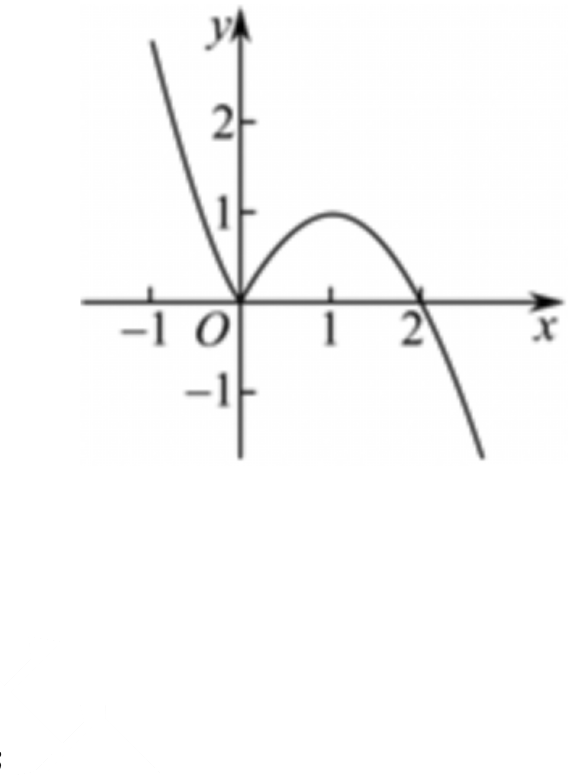
\includegraphics[width=0.20\textwidth]{figures/gao83_q15_graph.png}
\end{center}
\step{由 $[f(x)]^2+af(x)<0$ 得 $[f(x)+a]f(x)<0$，}
\step{当 $a=0$ 时，$[f(x)]^2<0$，不等式无解；}
\step{当 $a>0$ 时，由 $[f(x)+a]f(x)<0$ 得 $-a<f(x)<0$，}
\step{若不等式恰有 $1$ 个整数解，则整数解为 $3$，}
\step{又 $f(3)=-3$，$f(4)=-8$，所以 $-8\leqslant-a<-3$，所以 $3<a\leqslant8$；}
\step{当 $a<0$ 时，由 $[f(x)+a]f(x)<0$ 得 $0<f(x)<-a$，此时有多个解，故舍去；}
\step{综上所述，实数 $a$ 的取值范围为 $(3,8]$. 故选 $C$.}
\solend
\fi

\item 设函数 $f(x)=\begin{cases}\lvert2^x-1\rvert,&x\leqslant2\\ -x+7,&x>2\end{cases}$，若互不相等的实数 $a$、$b$、$c$ 满足 $f(a)=f(b)=f(c)$，
则 $2^a+2^b+2^c$ 的取值范围是\mbox{（\quad）}

\keepwithprev
A. $(8,9)$\qquad B. $(65,129)$\qquad C. $(64,128)$\qquad D. $(66,130)$

\ifanswer
\solbegin
\step{作出函数 $f(x)=\begin{cases}\lvert2^x-1\rvert,&x\leqslant2\\ -x+7,&x>2\end{cases}$ 的图象如图，}
\begin{center}
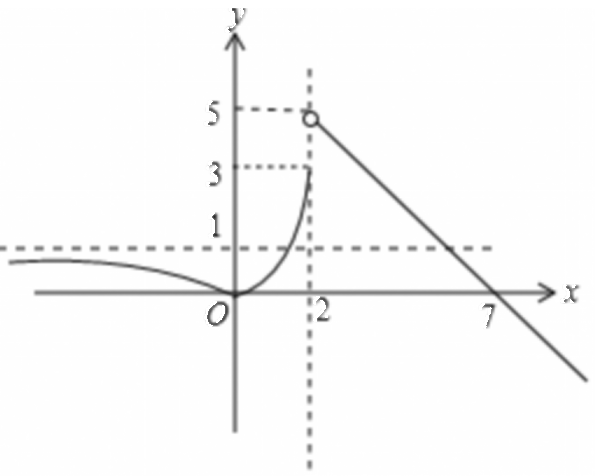
\includegraphics[width=0.22\textwidth]{figures/gao83_q16_graph.png}
\end{center}
\step{不妨设 $a<b<c$，由 $f(a)=f(b)$，得 $1-2^a=2^b-1$，则 $2^a+2^b=2$.}
\step{由 $f(-c)-c+6\in(0,1)$，得 $c\in(6,7)$，则 $64<2^c<128$，}
\step{所以 $66<2^a+2^b+2^c<130$，即 $2^a+2^b+2^c$ 的取值范围是 $(66,130)$. 故选 $D$.}
\solend
\fi

\end{enumerate}

\bigsec{三、解答题}

\begin{enumerate}
\setcounter{enumi}{16}

\item 已知幂函数 $f(x)$ 与一次函数 $g(x)$ 的图象都经过点 $(4,2)$，且 $f(9)=g(5)$.

（1）求 $f(x)$ 与 $g(x)$ 的解析式；

（2）求函数 $h(x)=g(x)-f(x)$ 在 $[0,4]$ 上的值域.

\ansspace*[8]

\ifanswer
\solbegin
\stepm{（1）}{设 $f(x)=x^\alpha$，$g(x)=kx+b$，则 $4^\alpha=2$，即 $\alpha=\dfrac12$，}
\step{$\begin{cases}4k+b=2\\ 3=5k+b\end{cases}$，则 $k=1$，$b=-2$，所以 $f(x)=\sqrt x$，$g(x)=x-2$；}
\stepm{（2）}{$h(x)=g(x)-f(x)=x-\sqrt x-2$，}
\step{令 $t=\sqrt x$，则 $t\in[0,2]$，原函数可化为 $p(t)=t^2-t-2$，}
\step{当 $t=\dfrac12$ 时，函数取得最小值 $-\dfrac94$，当 $t=2$ 时，函数取得最大值 $0$，}
\step{即函数值域为 $\left[-\dfrac94,0\right]$.}
\solend
\fi

\item 目前某县有 $100$ 万人. 经过 $x$ 年后为 $y$ 万人. 如果年平均增长率是 $1.2\%$. 请回答下列问题：

（1）写出 $y$ 关于 $x$ 的函数解析式.

（2）计算 $10$ 年后该县的人口总数（精确到 $0.1$ 万人）.

（3）计算大约多少年后该县的人口总数将达到 $120$ 万（精确到 $1$ 年）.

\ansspace*[9]

\ifanswer
\solbegin
\stepm{（1）}{当 $x=1$ 时，$y=100+100\times1.2\%=100(1+1.2\%)$，}
\step{当 $x=2$ 时，$y=100(1+1.2\%)+100(1+1.2\%)\times1.2\%=100(1+1.2\%)^2$，}
\step{当 $x=3$ 时，$y=100(1+1.2\%)^2+100(1+1.2\%)^2\times1.2\%=100(1+1.2\%)^3$，}
\step{$\cdots\cdots$}
\step{故 $y$ 关于 $x$ 的函数解析式为 $y=100(1+1.2\%)^x\,(x\in\N^*)$；}
\stepm{（2）}{当 $x=10$ 时，$y=100(1+1.2\%)^{10}=100\times1.012^{10}\approx112.7$，}
\step{故 $10$ 年后该县的人口总数约为 $112.7$ 万人；}
\stepm{（3）}{设 $x$ 年后该县的人口总数将达到 $120$ 万，即 $y=100(1+1.2\%)^x=120$，}
\step{解得 $x=\log_{1.012}\dfrac{120}{100}\approx16$，故大约 $16$ 年后该县的人口总数将达到 $120$ 万.}
\solend
\fi

\item 已知 $a>0$ 且 $a\neq1$，$m>0$，函数 $f(x)=(m^2+m-5)a^x$ 是指数函数，且 $f(2)=4$.

（1）求实数 $m$ 和 $a$ 的值；

（2）$f(2x)-2f(x)+2\geqslant nf(x)$ 对任意 $x\in[-1,2]$ 恒成立，求实数 $n$ 的取值范围；

（3）若关于 $x$ 的方程 $f(2x)-(2k+8)f(x)+2k+7b=0$ 有两个不相等的实数根，且一根
大于 $0$，另一根小于 $0$，其中 $k>0$，求整数 $b$ 的最大值.

\ansspace*[11]

\ifanswer
\solbegin
\stepm{（1）}{因为函数 $f(x)=(m^2+m-5)a^x$ 是指数函数，}
\step{所以 $m^2+m-5=1$，即 $m^2+m-6=0$，解得 $m=2$ 或 $m=-3$，}
\step{又 $m>0$，所以 $m=2$，又 $f(2)=a^2=4$，$a>0$ 且 $a\neq1$，所以 $a=2$；}
\stepm{（2）}{由（1）得 $f(x)=2^x$，}
\step{由题意 $2^{2x}-2\cdot2^x+2\geqslant n2^x$ 对任意 $x\in[-1,2]$ 恒成立，}
\step{所以 $n\leqslant2^x-2+\dfrac2{2^x}$ 对任意 $x\in[-1,2]$ 恒成立，则 $n\leqslant\left(2^x-2+\dfrac2{2^x}\right)_{\min}$，}
\step{记 $g(x)=2^x-2+\dfrac2{2^x}$，$x\in[-1,2]$，}
\step{令 $t=2^x$，因为 $x\in[-1,2]$，所以 $t\in\left[\dfrac12,4\right]$，则 $y=t+\dfrac2t-2$，$t\in\left[\dfrac12,4\right]$，}
\step{函数 $y=t+\dfrac2t-2$ 在 $\left[\dfrac12,\sqrt2\right]$ 上严格减，在 $[\sqrt2,4]$ 上严格增，}
\step{所以 $y=t+\dfrac2t-2$ 的最小值为 $\sqrt2+\dfrac2{\sqrt2}-2=2\sqrt2-2$，}
\step{所以 $n\leqslant2\sqrt2-2$，即实数 $n$ 的取值范围为 $(-\infty,2\sqrt2-2]$；}
\stepm{（3）}{方程 $f(2x)-(2k+8)f(x)+2k+7b=0$，}
\step{即方程 $2^{2x}-(2k+8)2^x+2k+7b=0$，即方程 $(2^x)^2-(2k+8)2^x+2k+7b=0$，}
\step{令 $t=2^x>0$，则方程 $t^2-(2k+8)t+2k+7b=0$，}
\step{因为关于 $x$ 的方程 $f(2x)-(2k+8)f(x)+2k+7b=0$ 的一根大于 $0$，另一根小于 $0$，}
\step{所以关于 $t$ 的方程 $t^2-(2k+8)t+2k+7b=0$ 的一根大于 $1$，另一根大于 $0$ 且小于 $1$，}
\step{记 $h(t)=t^2-(2k+8)t+2k+7b$，}
\step{所以 $\begin{cases}h(1)=1^2-(2k+8)\cdot1+2k+7b<0\\ h(0)=2k+7b>0\\ k>0\end{cases}$，所以 $\begin{cases}b<1\\ b>-\dfrac27k\\ k>0\end{cases}$，}
\step{所以整数 $b$ 的最大值为 $0$.}
\solend
\fi

\item 已知幂函数 $f(x)=(p^2-3p+3)x^{p^2-\frac32p-\frac12}$ 满足 $f(2)<f(4)$.

（1）求函数 $f(x)$ 的解析式；

（2）若函数 $g(x)=f^2(x)+mf(x)$，$x\in[1,9]$，是否存在实数 $m$ 使得 $g(x)$ 的最小值为 $0$？
若存在，求出 $m$ 的值；若不存在，说明理由.

（3）若函数 $h(x)=n-f(x+3)$，是否存在实数 $a$、$b\,(a<b)$，使函数 $h(x)$ 在 $[a,b]$ 上的
值域为 $[a,b]$？若存在，求出实数 $n$ 的取值范围；若不存在，说明理由.

\ansspace*[12]

\ifanswer
\solbegin
\stepm{（1）}{因为 $f(x)$ 是幂函数，所以 $p^2-3p+3=1$，解得 $p=1$ 或 $p=2$，}
\step{当 $p=1$ 时，$f(x)=\dfrac1x$，不满足 $f(2)<f(4)$.}
\step{当 $p=2$ 时，$f(x)=\sqrt x$，满足 $f(2)<f(4)$.}
\step{故 $p=2$，函数 $f(x)$ 的解析式为 $f(x)=\sqrt x$；}
\stepm{（2）}{由函数 $g(x)=f^2(x)+mf(x)$，即 $g(x)=(\sqrt x)^2+m\sqrt x$，}
\step{令 $t=\sqrt x$，因为 $x\in[1,9]$，所以 $t\in[1,3]$，}
\step{记 $k(x)=t^2+mt$，其对称轴 $t=-\dfrac m2$，}
\step{①当 $-\dfrac m2\leqslant1$，即 $m\geqslant-2$ 时，则 $k(x)_{\min}=k(1)=1+m=0$，解得 $m=-1$；}
\step{②当 $1<-\dfrac m2<3$ 时，即 $-6<m<-2$，则 $k(x)_{\min}=k\left(-\dfrac m2\right)=-\dfrac{m^2}4=0$，}
\step{解得 $m=0$，不满足，舍去；}
\step{③当 $-\dfrac m2\geqslant3$ 时，即 $m\leqslant-6$ 时，则 $k(x)_{\min}=k(3)=3m+9=0$，解得 $m=-3$，}
\step{不满足，舍去；}
\step{综上所述，存在 $m=-1$ 使得 $g(x)$ 的最小值为 $0$；}
\stepm{（3）}{由函数 $h(x)=n-f(x+3)=n-\sqrt{x+3}$ 在定义域内为严格减函数，}
\step{若存在实数 $a$、$b\,(a<b)$，使函数 $h(x)$ 在 $[a,b]$ 上的值域为 $[a,b]$，}
\step{则 $h(x)=\begin{cases}n-\sqrt{a+3}=b\text{ ①}\\ n-\sqrt{b+3}=a\text{ ②}\end{cases}$，}
\step{两式相减得 $\sqrt{a+3}-\sqrt{b+3}=a-b=(a+3)-(b+3)$，}
\step{所以 $\sqrt{a+3}+\sqrt{b+3}=1$ ③，}
\step{将③代入②得 $n=a+\sqrt{b+3}=a+1-\sqrt{a+3}$，}
\step{令 $t=\sqrt{a+3}$，因为 $a<b$，所以 $0\leqslant t<\dfrac12$，得 $n=t^2-t-2=\left(t-\dfrac12\right)^2-\dfrac94$，}
\step{故实数 $n$ 的取值范围为 $\left(-\dfrac94,-2\right]$.}
\solend
\fi

\item 定理（三角不等式），对于任意的 $a$、$b\in\R$，恒有 $\bigl\lvert\lvert a\rvert-\lvert b\rvert\bigr\rvert\leqslant\lvert a\pm b\rvert\leqslant\lvert a\rvert+\lvert b\rvert$. 定义：
已知 $n\in\N$ 且 $n\geqslant3$，对于有序数组 $a_1$、$a_2$、$\cdots$、$a_n$，称 $\lvert a_1-a_2\rvert+\lvert a_2-a_3\rvert+\cdots+\lvert a_{n-1}-a_n\rvert$
为有序数组 $a_1$、$a_2$、$\cdots$、$a_n$ 的波动距离，记作 $f(a_1,a_2,\cdots,a_n)$，即
$f(a_1,a_2,\cdots,a_n)=\lvert a_1-a_2\rvert+\lvert a_2-a_3\rvert+\cdots+\lvert a_{n-1}-a_n\rvert$，请根据上述信息解决以下几个问题：

（1）求函数 $y=\lvert x-2\rvert+\lvert x-4\rvert$ 的最小值，并指出函数取到最小值时 $x$ 的取值范围；

（2）①求有序数组 $2$、$5$、$3$、$4$ 的波动距离 $f(2,5,3,4)$；

②求证：若 $a$、$b$、$c$、$d\in\R$ 且 $a<b<c$，则 $f(a,b,c,d)\leqslant f(a,c,b,d)$；

（3）同理可证得命题“若 $a$、$b$、$c$、$d\in\R$ 且 $c<b<a$ 时，$f(a,b,c,d)\leqslant f(a,c,b,d)$”也
是真命题（注：该命题无需证明，需要时可直接使用）.

设两两不相等的四个实数 $a_1$、$a_2$、$a_3$、$a_4\in\{3^1,3^2,3^3,3^4\}$，求有序数组 $a_1$、$a_2$、$a_3$、$a_4$ 的
波动距离 $f(a_1,a_2,a_3,a_4)$ 的最大值.

\ansspace*[14]

\ifanswer
\solbegin
\stepm{（1）}{由三角不等式得 $\bigl\lvert\lvert a\rvert-\lvert b\rvert\bigr\rvert\leqslant\lvert a\pm b\rvert\leqslant\lvert a\rvert+\lvert b\rvert$，}
\step{当且仅当 $\lvert a+b\rvert^2=(\lvert a\rvert+\lvert b\rvert)^2$ 时，}
\step{即当 $-ab=\lvert ab\rvert$ 时，即当 $ab\leqslant0$ 时取等号，}
\step{由三角不等式得 $y=\lvert x-2\rvert+\lvert x-4\rvert\geqslant\lvert(x-2)-(x-4)\rvert=2$，}
\step{当且仅当 $(x-2)(x-4)\leqslant0$ 时，即 $2\leqslant x\leqslant4$ 时取等号，}
\step{因此，函数 $y=\lvert x-2\rvert+\lvert x-4\rvert$ 的最小值为 $2$，此时 $x$ 的取值范围是 $[2,4]$.}
\stepm{（2）}{①由题中定义得 $f(2,5,3,4)=\lvert2-5\rvert+\lvert5-3\rvert+\lvert3-4\rvert=6$；}
\step{②$f(a,b,c,d)-f(a,c,b,d)=\lvert a-b\rvert+\lvert c-d\rvert-\lvert a-c\rvert-\lvert b-d\rvert$，}
\step{因为 $a<b<c$，所以 $\lvert a-b\rvert-\lvert a-c\rvert=-\lvert b-c\rvert$，$\lvert c-d\rvert-\lvert b-d\rvert\leqslant\lvert b-c\rvert$，}
\step{所以 $f(a,b,c,d)-f(a,c,b,d)\leqslant0$，即 $f(a,b,c,d)\leqslant f(a,c,b,d)$，}
\stepm{（3）}{$f(a,b,c,d)=\lvert a-b\rvert+\lvert b-c\rvert+\lvert c-d\rvert$}
\step{$=\lvert d-c\rvert+\lvert c-b\rvert+\lvert b-a\rvert=f(d,c,b,a)$，}
\step{当 $f(a_1,a_2,a_3,a_4)$ 取得最大值时，$a_2=\max\{a_1,a_2,a_3\}$ 或 $a_2=\min\{a_1,a_2,a_3\}$，}
\step{同理 $a_3=\max\{a_2,a_3,a_4\}$ 或 $a_3=\min\{a_2,a_3,a_4\}$，}
\step{若 $a_2=\max\{a_1,a_2,a_3\}$，则 $a_2>a_3$，所以 $a_3=\min\{a_2,a_3,a_4\}$，}
\step{故 $f(a_1,a_2,a_3,a_4)=\lvert a_1-a_2\rvert+\lvert a_2-a_3\rvert+\lvert a_3-a_4\rvert=a_2-a_1+a_2-a_3+a_4-a_3$}
\step{$=2a_2+a_4-2a_3-a_1\leqslant2\times3^4+3^3-2\times3^1-3^2=174$，}
\step{当且仅当 $a_1=3^2$，$a_2=3^4$，$a_3=3^1$，$a_4=3^3$ 时取等号，}
\step{所以 $f(3^2,3^4,3^1,3^3)$ 为 $f(a_1,a_2,a_3,a_4)$ 的最大值，}
\step{若 $a_2=\min\{a_1,a_2,a_3\}$，则 $a_2<a_3$，所以 $a_3=\max\{a_2,a_3,a_4\}$，}
\step{同理可得 $f(3^3,3^4,3^1,3^2)$ 为 $f(a_1,a_2,a_3,a_4)$ 的最大值，}
\step{综上所述，$f(a_1,a_2,a_3,a_4)$ 的最大值为 $174$.}
\solend
\fi

\end{enumerate}

\end{document}
"
% 紧凑版：xelatex "\def\iscompact{1}% 高一83_交附闵行_周末作业10.23.tex
%   —— 高一上数学“2026-2027 年交附闵行高一上周末作业 10.23”（讲评版）
% 试卷版：xelatex 高一83_交附闵行_周末作业10.23.tex
% 答案版：xelatex "\def\isanswer{1}\input{高一83_交附闵行_周末作业10.23.tex}"
% 紧凑版：xelatex "\def\iscompact{1}\input{高一83_交附闵行_周末作业10.23.tex}"
%
% 原始材料：微信公众号“魔都数学加油站”文章，连载“27学年高一83”；
% 原文标题“27学年高一83——2026-2027年上海市交附闵行高一上周末作业10.23”；
% 原文链接：https://mp.weixin.qq.com/s/t5AfTwQXg4Sj4i_Dl5rgXA。
% 页面标注发布时间 2026-10-26 20:15（上海）。
% 正文为 12 张 PNG 页（`原图/高一83_交附闵行_周末作业10.23/01..12.png`），
% 尺寸混排（第 1—8 页为 4762×6735，第 9—12 页为 2560×3620），均按页序读取。
%
% 篇幅与题号：原卷自第 3 题起编号（第 1、2 题不在原文内）。填空题 3—12（10 题）、
% 选择题 13—16（4 题）、解答题 17—21（5 题），共 19 题。
%
% 讲评版：19 题全部印【解析】，本稿不另提 \ans{}；选择题答案在解析末句“故选 C／B／C／D”。
%
% 副标题：原卷未印副标题。本稿按内容标作“函数与导数”（本卷考幂函数、指数函数、
% 对数与函数应用，属“函数与导数”模块；副标题只用知识模块名，见 README 说明）。
%
% 与原卷的排版差异：
%   ① 原卷每题下直接印【解析】，本稿按全稿惯例将解析置于答案版；
%   ② 原卷未印副标题，本稿补出；填空横线统一排 \blankline[4.4em]；
%   ③ 原卷数集记号排斜体 $R$、$Z$、$N$，本稿按全稿惯例改用 $\R$、$\Z$、$\N$；
%   ④ 第 17—21 题的子问用行内“（1）（2）（3）”段，解析中的子问标号用 \stepm；
%   ⑤ 解答题按惯例加 \ansspace；选择题括号排 \mbox{（\quad）}；
%   ⑥ 第 15、16 题解析各有一幅函数图象，裁自原图（第 6 页）后去粉色水印、转灰度，
%      仅答案版出。
%
% 行数核对：逐题数 \step/\stepm 条数，合计 145 条（Q3：1；Q4：1；Q5：4；Q6：5；
% Q7：2；Q8：7；Q9：10；Q10：5；Q11：6；Q12：8；Q13：3；Q14：4；Q15：8；
% Q16：4；Q17：6；Q18：9；Q19：19；Q20：21；Q21：22）。原卷解析的换行
% 按语意合并，未逐行强拆。
%
\documentclass[a4paper,11pt]{article}
\usepackage{common}

\begin{document}

\examtitlest[4]{2026--2027 年交附闵行高一上周末作业 10.23}{函数与导数}

\bigsec{一、填空题}

\begin{enumerate}
\setcounter{enumi}{2}

\item 已知 $10^a=2$，$10^b=5$，则 $10^{3a-2b}$ 的值为\blankline[4.4em].

\ifanswer
\solbegin
\step{$10^{3a-2b}=\dfrac{10^{3a}}{10^{2b}}=\dfrac{(10^a)^3}{(10^b)^2}=\dfrac{2^3}{5^2}=\dfrac8{25}$.}
\solend
\fi

\item 根式 $a\sqrt{-a}$ 化成分数指数幂是\blankline[4.4em].

\ifanswer
\solbegin
\step{$a\sqrt{-a}=a(-a)^{\frac12}=-(-a)(-a)^{\frac12}=-(-a)^{\frac32}$.}
\solend
\fi

\item 已知数列 $\{a_n\}$ 的通项公式为 $a_n=\left(\dfrac49\right)^{n-1}-\left(\dfrac23\right)^{n-1}$，在下列说法中：①有最大项；
②有最小项；③没有最大项；④没有最小项. 正确的是\blankline[3.6em]（填序号）.

\ifanswer
\solbegin
\step{令 $t=\left(\dfrac23\right)^{n-1}$，则 $t\in\left\{1,\dfrac23,\dfrac49,\dfrac8{27},\cdots\right\}\subset(0,1]$，$t$ 是关于 $n$ 的减函数，}
\step{则 $a_n=t^2-t=\left(t-\dfrac12\right)^2-\dfrac14$，}
\step{所以当 $t=1$ 即 $n=1$ 时 $a_n$ 取得最大为 $0$，当 $t=\dfrac49$ 即 $n=3$ 时 $a_n$ 取得最小为 $-\dfrac{20}{81}$，}
\step{所以 $a_n$ 既有最大项又有最小项，故①和②正确.}
\solend
\fi

\item 已知 $f(x)=\mathrm{e}^{x-\frac12}-\mathrm{e}^{-x+\frac12}+\dfrac{4x}{2x-1}$，则
$f\left(\dfrac1{2020}\right)+f\left(\dfrac2{2020}\right)+f\left(\dfrac3{2020}\right)+\cdots+f\left(\dfrac{1009}{2020}\right)+f\left(\dfrac{1011}{2020}\right)+\cdots+f\left(\dfrac{2019}{2020}\right)$ 的
值为\blankline[4.4em].

\ifanswer
\solbegin
\step{因为 $f(x)+f(1-x)=\mathrm{e}^{x-\frac12}-\mathrm{e}^{-x+\frac12}+\dfrac{4x}{2x-1}+\mathrm{e}^{(1-x)-\frac12}-\mathrm{e}^{-(1-x)+\frac12}+\dfrac{4(1-x)}{2(1-x)-1}$}
\step{$=\dfrac{4x}{2x-1}+\dfrac{4-4x}{1-2x}=\dfrac{4(2x-1)}{2x-1}=4$，}
\step{记 $S=f\left(\dfrac1{2020}\right)+f\left(\dfrac2{2020}\right)+\cdots+f\left(\dfrac{2019}{2020}\right)$，}
\step{又 $S=f\left(\dfrac{2019}{2020}\right)+f\left(\dfrac{2018}{2020}\right)+\cdots+f\left(\dfrac2{2020}\right)+f\left(\dfrac1{2020}\right)$，}
\step{对齐相加得 $2S=2018\times4$，所以 $S=4036$.}
\solend
\fi

\item 不等式 $2^{x^2-2x-3}<\left(\dfrac12\right)^{3(x-1)}$ 的解集为\blankline[4.4em].

\ifanswer
\solbegin
\step{由 $2^{x^2-2x-3}<\left(\dfrac12\right)^{3(x-1)}$ 得 $x^2-2x-3<-3(x-1)$，即 $x^2+x-6<0$，}
\step{故解集为 $(-3,2)$.}
\solend
\fi

\item 函数 $f(x)=x^{\ln5}+x^{\ln12}-13^{\ln x}$ 的零点是\blankline[4.4em]. 附：$a^{\log_bc}=c^{\log_ba}$
（$a>0$，$b>0$，$c>0$，$b\neq1$）.

\ifanswer
\solbegin
\step{函数 $f(x)=x^{\ln5}+x^{\ln12}-13^{\ln x}$，}
\step{若 $f(x)=x^{\ln5}+x^{\ln12}-13^{\ln x}=0$，变形得 $x^{\ln5}+x^{\ln12}=13^{\ln x}$，}
\step{又 $a^{\log_bc}=c^{\log_ba}$（$a>0$，$b>0$，$c>0$，$b\neq1$），得 $5^{\ln x}+12^{\ln x}=13^{\ln x}$，}
\step{令 $g(t)=\left(\dfrac5{13}\right)^t+\left(\dfrac{12}{13}\right)^t-1$，易得 $g(t)$ 严格减，所以 $g(t)=0$ 至多有一解，}
\step{即 $\left(\dfrac5{13}\right)^t+\left(\dfrac{12}{13}\right)^t-1=0$ 至多有一解，变形得方程 $5^t+12^t=13^t$ 至多有一解，}
\step{易得 $t=2$ 时，有 $5^2+12^2=13^2$ 成立，则方程 $5^t+12^t=13^t$ 有唯一解 $t=2$，}
\step{即 $\ln x=2$，解得 $x=\mathrm{e}^2$，即函数 $f(x)$ 的零点为 $\mathrm{e}^2$.}
\solend
\fi

\item 已知幂函数 $f(x)=(m^2-2m-2)x^{m^2+m-2}$ 在 $(0,+\infty)$ 上是严格减函数，则不等式
$f(x-1)<f(3-2x)$ 的解集为\blankline[4.4em].

\ifanswer
\solbegin
\step{因为 $f(x)$ 为幂函数，所以 $m^2-2m-2=1$，解得 $m=-1$ 或 $m=3$；}
\step{当 $m=3$ 时，$f(x)=x^{10}$ 在 $(0,+\infty)$ 上严格增，不合题意；}
\step{当 $m=-1$ 时，$f(x)=x^{-2}$ 在 $(0,+\infty)$ 上严格减，符合题意；}
\step{综上所述，$m=-1$；}
\step{因为 $f(x)=x^{-2}$ 的定义域为 $(-\infty,0)\cup(0,+\infty)$，$f(-x)=(-x)^{-2}=x^{-2}=f(x)$，}
\step{所以 $f(x)$ 为定义在 $(-\infty,0)\cup(0,+\infty)$ 上的偶函数，}
\step{故 $f(x-1)=f(\lvert x-1\rvert)$，$f(3-2x)=f(\lvert3-2x\rvert)$，}
\step{$f(x-1)<f(3-2x)\Rightarrow f(\lvert x-1\rvert)<f(\lvert3-2x\rvert)\Rightarrow\lvert x-1\rvert>\lvert3-2x\rvert$}
\step{且 $\lvert x-1\rvert\neq0$，$\lvert3-2x\rvert\neq0$，解得 $\dfrac43<x<\dfrac32$ 或 $\dfrac32<x<2$，}
\step{所以 $f(x-1)<f(3-2x)$ 的解集为 $\left(\dfrac43,\dfrac32\right)\cup\left(\dfrac32,2\right)$.}
\solend
\fi

\item 若实数 $x_1$、$x_2$ 满足 $\mathrm{e}^{x_1}+x_1-3=0$，$x_2\ln x_2+3x_2-1=0$，则 $\dfrac{x_1x_2+1}{x_2}$ 的值为\blankline[4.4em].

\ifanswer
\solbegin
\step{易得 $x_2>0$，则 $\ln x_2+3-\dfrac1{x_2}=0$，即 $\mathrm{e}^{-\ln x_2}+(-\ln x_2)-3=0$.}
\step{设 $f(x)=\mathrm{e}^x+x-3$，则函数 $f(x)$ 在 $(-\infty,+\infty)$ 上严格增.}
\step{由 $\mathrm{e}^{x_1}+x_1-3=0$，$\mathrm{e}^{-\ln x_2}+(-\ln x_2)-3=0$，得 $f(x_1)=0$，$f(-\ln x_2)=0$，}
\step{所以 $f(x_1)=f(-\ln x_2)$，得 $x_1=-\ln x_2$，即 $\ln x_2=-x_1$，所以 $x_2=\mathrm{e}^{-x_1}$，得 $\dfrac1{x_2}=\mathrm{e}^{x_1}$.}
\step{因为 $\mathrm{e}^{x_1}+x_1-3=0$，所以 $\mathrm{e}^{x_1}+x_1=3$，所以 $\dfrac{x_1x_2+1}{x_2}=x_1+\dfrac1{x_2}=\mathrm{e}^{x_1}+x_1=3$.}
\solend
\fi

\item 已知 $\alpha$、$\beta$ 是方程 $9^x-2m\cdot3^x+m^2-1=0$ 的两个根，若 $\alpha+\beta=1$，则 $\alpha\beta=\blankline[4.4em]$.

\ifanswer
\solbegin
\step{由题意得方程 $9^x-2m\cdot3^x+m^2-1=0$ 有两个根，}
\step{则方程 $t^2-2mt+m^2-1=0$ 有二正根，则 $\begin{cases}\Delta=4m^2-4(m^2-1)\geqslant0\\ 2m>0\\ m^2-1>0\end{cases}$，解得 $m>1$，}
\step{又 $\alpha$、$\beta$ 是方程 $9^x-2m\cdot3^x+m^2-1=0$ 的两个根，则 $3^\alpha\times3^\beta=m^2-1$，}
\step{又 $\alpha+\beta=1$，则 $m^2-1=3^{\alpha+\beta}=3$，解得 $m=2$ 或 $m=-2$（舍），}
\step{则 $3^\alpha+3^\beta=2m=4$，又 $\alpha=1-\beta$，则 $3^{1-\beta}+3^\beta=4$，解得 $\beta=0$ 或 $\beta=1$，}
\step{则 $\begin{cases}\alpha=1\\ \beta=0\end{cases}$ 或 $\begin{cases}\alpha=0\\ \beta=1\end{cases}$，则 $\alpha\beta=0$.}
\solend
\fi

\item 已知实数 $a,b,c\in(1,+\infty)$，满足 $a^{\log_ba}\cdot b^{\log_cb}\cdot c^{\log_ac}=100$，则 $abc$ 的最大值为\blankline[4.4em].

\ifanswer
\solbegin
\step{由换底公式得 $\log_ba=\dfrac{\ln a}{\ln b}$，$\log_cb=\dfrac{\ln b}{\ln c}$，$\log_ac=\dfrac{\ln c}{\ln a}$，}
\step{设 $X=\ln a$，$Y=\ln b$，$Z=\ln c$，得 $a=\mathrm{e}^X$，$b=\mathrm{e}^Y$，$c=\mathrm{e}^Z$，}
\step{代入得 $a^{\log_ba}\cdot b^{\log_cb}\cdot c^{\log_ac}=a^{\frac{\ln a}{\ln b}}\cdot b^{\frac{\ln b}{\ln c}}\cdot c^{\frac{\ln c}{\ln a}}=(\mathrm{e}^X)^{\frac XY}\cdot(\mathrm{e}^Y)^{\frac YZ}\cdot(\mathrm{e}^Z)^{\frac ZX}=100$，}
\step{即 $\mathrm{e}^{\frac{X^2}Y+\frac{Y^2}Z+\frac{Z^2}X}=100$，两边取对数得 $\dfrac{X^2}Y+\dfrac{Y^2}Z+\dfrac{Z^2}X=\ln100$.}
\step{由 $a,b,c\in(1,+\infty)$，得 $X>0$，$Y>0$，$Z>0$，}
\step{由柯西不等式，得 $\left(\dfrac{X^2}Y+\dfrac{Y^2}Z+\dfrac{Z^2}X\right)(X+Y+Z)\geqslant(X+Y+Z)^2$，}
\step{即 $X+Y+Z\leqslant\dfrac{X^2}Y+\dfrac{Y^2}Z+\dfrac{Z^2}X=\ln100$，当且仅当 $X=Y=Z$ 时取等号，}
\step{因此 $(X+Y+Z)_{\max}=\ln100$，所以 $(abc)_{\max}=\mathrm{e}^{(X+Y+Z)_{\max}}=\mathrm{e}^{\ln100}=100$.}
\solend
\fi

\end{enumerate}

\bigsec{二、选择题}

\begin{enumerate}
\setcounter{enumi}{12}

\item 已知集合 $A=\{x\mid x=2k,k\in\Z\}$，$B=\{x\mid x=4k+2,\,k\in\Z\}$，则 $A\cup B=\mbox{（\quad）}$

\keepwithprev
A. $B$\qquad B. $\R$\qquad C. $A$\qquad D. 以上都不是

\ifanswer
\solbegin
\step{$B=\{x\mid x=4k+2,k\in\Z\}=\{x\mid x=2(2k+1),k\in\Z\}$，它表示奇数的 $2$ 倍组成的集合，}
\step{$A=\{x\mid x=2k,k\in\Z\}$，即集合 $A$ 是整数的 $2$ 倍组成的集合，}
\step{则 $B\subseteq A$，则 $A\cup B=A$. 故选 $C$.}
\solend
\fi

\item 教室通风的目的是通过空气的流动，排出室内的污浊空气和致病微生物，降低室内二氧化碳和致病微生物的浓度，送进室外的新鲜空气. 按照国家标准，教室内空气中二氧化碳日平均最高容许浓度应小于等于 $0.1\%$. 经测定，刚下课时，空气中含有 $0.2\%$ 的二氧化碳，若开窗通风后教室内二氧化碳的浓度为 $y\%$，且 $y$ 随时间 $t$（单位：分钟）的变化规律可以用函数 $y=0.05+\lambda\mathrm{e}^{-\frac t{12}}\,(\lambda\in\R)$ 描述，则该教室内的二氧化碳浓度达到国家标准至少需要的时间为\mbox{（\quad）}

\keepwithprev
A. $10$ 分钟\qquad B. $14$ 分钟\qquad C. $15$ 分钟\qquad D. $20$ 分钟

\ifanswer
\solbegin
\step{由题意得，当 $t=0$ 时，$y=0.2$，即 $0.05+\lambda\mathrm{e}^0=0.2$，解得 $\lambda=0.15$，}
\step{所以 $y=0.05+0.15\mathrm{e}^{-\frac t{12}}$，由题意得 $0.05+0.15\mathrm{e}^{-\frac t{12}}\leqslant0.1$，即 $\mathrm{e}^{-\frac t{12}}\leqslant\dfrac13$，}
\step{两边取对数得 $-\dfrac t{12}\leqslant-\ln3$，所以 $t\geqslant12\ln3\approx13.2$，}
\step{所以该教室内的二氧化碳浓度达到国家标准至少需要的时间为 $14$ 分钟. 故选 $B$.}
\solend
\fi

\item 已知函数 $f(x)=\begin{cases}-x^2+2x,&x\geqslant0\\ x^2-2x,&x<0\end{cases}$，若关于 $x$ 的不等式 $[f(x)]^2+af(x)<0$ 恰有 $1$ 个整数
解，则实数 $a$ 的最大值为\mbox{（\quad）}

\keepwithprev
A. $-2$\qquad B. $3$\qquad C. $8$\qquad D. $9$

\ifanswer
\solbegin
\step{作出 $f(x)$ 的图象，如图所示：}
\begin{center}
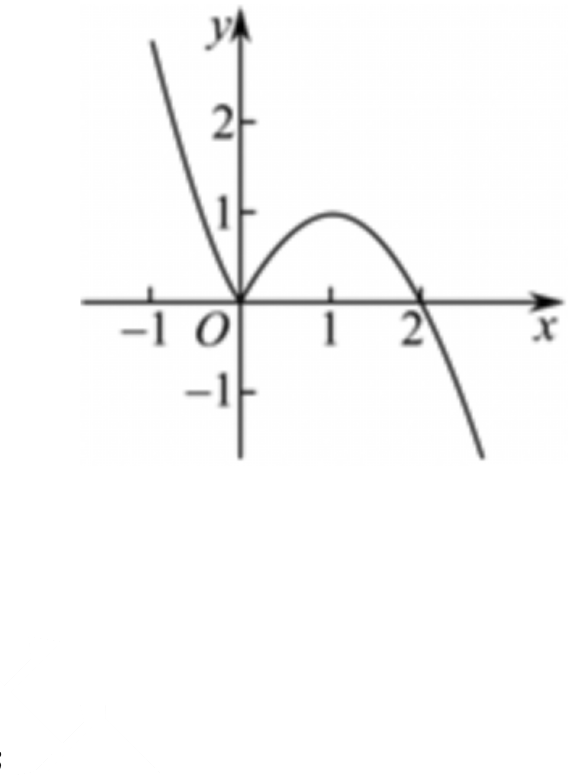
\includegraphics[width=0.20\textwidth]{figures/gao83_q15_graph.png}
\end{center}
\step{由 $[f(x)]^2+af(x)<0$ 得 $[f(x)+a]f(x)<0$，}
\step{当 $a=0$ 时，$[f(x)]^2<0$，不等式无解；}
\step{当 $a>0$ 时，由 $[f(x)+a]f(x)<0$ 得 $-a<f(x)<0$，}
\step{若不等式恰有 $1$ 个整数解，则整数解为 $3$，}
\step{又 $f(3)=-3$，$f(4)=-8$，所以 $-8\leqslant-a<-3$，所以 $3<a\leqslant8$；}
\step{当 $a<0$ 时，由 $[f(x)+a]f(x)<0$ 得 $0<f(x)<-a$，此时有多个解，故舍去；}
\step{综上所述，实数 $a$ 的取值范围为 $(3,8]$. 故选 $C$.}
\solend
\fi

\item 设函数 $f(x)=\begin{cases}\lvert2^x-1\rvert,&x\leqslant2\\ -x+7,&x>2\end{cases}$，若互不相等的实数 $a$、$b$、$c$ 满足 $f(a)=f(b)=f(c)$，
则 $2^a+2^b+2^c$ 的取值范围是\mbox{（\quad）}

\keepwithprev
A. $(8,9)$\qquad B. $(65,129)$\qquad C. $(64,128)$\qquad D. $(66,130)$

\ifanswer
\solbegin
\step{作出函数 $f(x)=\begin{cases}\lvert2^x-1\rvert,&x\leqslant2\\ -x+7,&x>2\end{cases}$ 的图象如图，}
\begin{center}
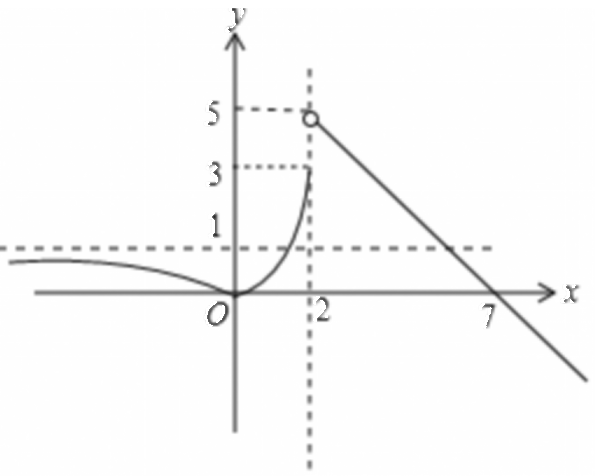
\includegraphics[width=0.22\textwidth]{figures/gao83_q16_graph.png}
\end{center}
\step{不妨设 $a<b<c$，由 $f(a)=f(b)$，得 $1-2^a=2^b-1$，则 $2^a+2^b=2$.}
\step{由 $f(-c)-c+6\in(0,1)$，得 $c\in(6,7)$，则 $64<2^c<128$，}
\step{所以 $66<2^a+2^b+2^c<130$，即 $2^a+2^b+2^c$ 的取值范围是 $(66,130)$. 故选 $D$.}
\solend
\fi

\end{enumerate}

\bigsec{三、解答题}

\begin{enumerate}
\setcounter{enumi}{16}

\item 已知幂函数 $f(x)$ 与一次函数 $g(x)$ 的图象都经过点 $(4,2)$，且 $f(9)=g(5)$.

（1）求 $f(x)$ 与 $g(x)$ 的解析式；

（2）求函数 $h(x)=g(x)-f(x)$ 在 $[0,4]$ 上的值域.

\ansspace*[8]

\ifanswer
\solbegin
\stepm{（1）}{设 $f(x)=x^\alpha$，$g(x)=kx+b$，则 $4^\alpha=2$，即 $\alpha=\dfrac12$，}
\step{$\begin{cases}4k+b=2\\ 3=5k+b\end{cases}$，则 $k=1$，$b=-2$，所以 $f(x)=\sqrt x$，$g(x)=x-2$；}
\stepm{（2）}{$h(x)=g(x)-f(x)=x-\sqrt x-2$，}
\step{令 $t=\sqrt x$，则 $t\in[0,2]$，原函数可化为 $p(t)=t^2-t-2$，}
\step{当 $t=\dfrac12$ 时，函数取得最小值 $-\dfrac94$，当 $t=2$ 时，函数取得最大值 $0$，}
\step{即函数值域为 $\left[-\dfrac94,0\right]$.}
\solend
\fi

\item 目前某县有 $100$ 万人. 经过 $x$ 年后为 $y$ 万人. 如果年平均增长率是 $1.2\%$. 请回答下列问题：

（1）写出 $y$ 关于 $x$ 的函数解析式.

（2）计算 $10$ 年后该县的人口总数（精确到 $0.1$ 万人）.

（3）计算大约多少年后该县的人口总数将达到 $120$ 万（精确到 $1$ 年）.

\ansspace*[9]

\ifanswer
\solbegin
\stepm{（1）}{当 $x=1$ 时，$y=100+100\times1.2\%=100(1+1.2\%)$，}
\step{当 $x=2$ 时，$y=100(1+1.2\%)+100(1+1.2\%)\times1.2\%=100(1+1.2\%)^2$，}
\step{当 $x=3$ 时，$y=100(1+1.2\%)^2+100(1+1.2\%)^2\times1.2\%=100(1+1.2\%)^3$，}
\step{$\cdots\cdots$}
\step{故 $y$ 关于 $x$ 的函数解析式为 $y=100(1+1.2\%)^x\,(x\in\N^*)$；}
\stepm{（2）}{当 $x=10$ 时，$y=100(1+1.2\%)^{10}=100\times1.012^{10}\approx112.7$，}
\step{故 $10$ 年后该县的人口总数约为 $112.7$ 万人；}
\stepm{（3）}{设 $x$ 年后该县的人口总数将达到 $120$ 万，即 $y=100(1+1.2\%)^x=120$，}
\step{解得 $x=\log_{1.012}\dfrac{120}{100}\approx16$，故大约 $16$ 年后该县的人口总数将达到 $120$ 万.}
\solend
\fi

\item 已知 $a>0$ 且 $a\neq1$，$m>0$，函数 $f(x)=(m^2+m-5)a^x$ 是指数函数，且 $f(2)=4$.

（1）求实数 $m$ 和 $a$ 的值；

（2）$f(2x)-2f(x)+2\geqslant nf(x)$ 对任意 $x\in[-1,2]$ 恒成立，求实数 $n$ 的取值范围；

（3）若关于 $x$ 的方程 $f(2x)-(2k+8)f(x)+2k+7b=0$ 有两个不相等的实数根，且一根
大于 $0$，另一根小于 $0$，其中 $k>0$，求整数 $b$ 的最大值.

\ansspace*[11]

\ifanswer
\solbegin
\stepm{（1）}{因为函数 $f(x)=(m^2+m-5)a^x$ 是指数函数，}
\step{所以 $m^2+m-5=1$，即 $m^2+m-6=0$，解得 $m=2$ 或 $m=-3$，}
\step{又 $m>0$，所以 $m=2$，又 $f(2)=a^2=4$，$a>0$ 且 $a\neq1$，所以 $a=2$；}
\stepm{（2）}{由（1）得 $f(x)=2^x$，}
\step{由题意 $2^{2x}-2\cdot2^x+2\geqslant n2^x$ 对任意 $x\in[-1,2]$ 恒成立，}
\step{所以 $n\leqslant2^x-2+\dfrac2{2^x}$ 对任意 $x\in[-1,2]$ 恒成立，则 $n\leqslant\left(2^x-2+\dfrac2{2^x}\right)_{\min}$，}
\step{记 $g(x)=2^x-2+\dfrac2{2^x}$，$x\in[-1,2]$，}
\step{令 $t=2^x$，因为 $x\in[-1,2]$，所以 $t\in\left[\dfrac12,4\right]$，则 $y=t+\dfrac2t-2$，$t\in\left[\dfrac12,4\right]$，}
\step{函数 $y=t+\dfrac2t-2$ 在 $\left[\dfrac12,\sqrt2\right]$ 上严格减，在 $[\sqrt2,4]$ 上严格增，}
\step{所以 $y=t+\dfrac2t-2$ 的最小值为 $\sqrt2+\dfrac2{\sqrt2}-2=2\sqrt2-2$，}
\step{所以 $n\leqslant2\sqrt2-2$，即实数 $n$ 的取值范围为 $(-\infty,2\sqrt2-2]$；}
\stepm{（3）}{方程 $f(2x)-(2k+8)f(x)+2k+7b=0$，}
\step{即方程 $2^{2x}-(2k+8)2^x+2k+7b=0$，即方程 $(2^x)^2-(2k+8)2^x+2k+7b=0$，}
\step{令 $t=2^x>0$，则方程 $t^2-(2k+8)t+2k+7b=0$，}
\step{因为关于 $x$ 的方程 $f(2x)-(2k+8)f(x)+2k+7b=0$ 的一根大于 $0$，另一根小于 $0$，}
\step{所以关于 $t$ 的方程 $t^2-(2k+8)t+2k+7b=0$ 的一根大于 $1$，另一根大于 $0$ 且小于 $1$，}
\step{记 $h(t)=t^2-(2k+8)t+2k+7b$，}
\step{所以 $\begin{cases}h(1)=1^2-(2k+8)\cdot1+2k+7b<0\\ h(0)=2k+7b>0\\ k>0\end{cases}$，所以 $\begin{cases}b<1\\ b>-\dfrac27k\\ k>0\end{cases}$，}
\step{所以整数 $b$ 的最大值为 $0$.}
\solend
\fi

\item 已知幂函数 $f(x)=(p^2-3p+3)x^{p^2-\frac32p-\frac12}$ 满足 $f(2)<f(4)$.

（1）求函数 $f(x)$ 的解析式；

（2）若函数 $g(x)=f^2(x)+mf(x)$，$x\in[1,9]$，是否存在实数 $m$ 使得 $g(x)$ 的最小值为 $0$？
若存在，求出 $m$ 的值；若不存在，说明理由.

（3）若函数 $h(x)=n-f(x+3)$，是否存在实数 $a$、$b\,(a<b)$，使函数 $h(x)$ 在 $[a,b]$ 上的
值域为 $[a,b]$？若存在，求出实数 $n$ 的取值范围；若不存在，说明理由.

\ansspace*[12]

\ifanswer
\solbegin
\stepm{（1）}{因为 $f(x)$ 是幂函数，所以 $p^2-3p+3=1$，解得 $p=1$ 或 $p=2$，}
\step{当 $p=1$ 时，$f(x)=\dfrac1x$，不满足 $f(2)<f(4)$.}
\step{当 $p=2$ 时，$f(x)=\sqrt x$，满足 $f(2)<f(4)$.}
\step{故 $p=2$，函数 $f(x)$ 的解析式为 $f(x)=\sqrt x$；}
\stepm{（2）}{由函数 $g(x)=f^2(x)+mf(x)$，即 $g(x)=(\sqrt x)^2+m\sqrt x$，}
\step{令 $t=\sqrt x$，因为 $x\in[1,9]$，所以 $t\in[1,3]$，}
\step{记 $k(x)=t^2+mt$，其对称轴 $t=-\dfrac m2$，}
\step{①当 $-\dfrac m2\leqslant1$，即 $m\geqslant-2$ 时，则 $k(x)_{\min}=k(1)=1+m=0$，解得 $m=-1$；}
\step{②当 $1<-\dfrac m2<3$ 时，即 $-6<m<-2$，则 $k(x)_{\min}=k\left(-\dfrac m2\right)=-\dfrac{m^2}4=0$，}
\step{解得 $m=0$，不满足，舍去；}
\step{③当 $-\dfrac m2\geqslant3$ 时，即 $m\leqslant-6$ 时，则 $k(x)_{\min}=k(3)=3m+9=0$，解得 $m=-3$，}
\step{不满足，舍去；}
\step{综上所述，存在 $m=-1$ 使得 $g(x)$ 的最小值为 $0$；}
\stepm{（3）}{由函数 $h(x)=n-f(x+3)=n-\sqrt{x+3}$ 在定义域内为严格减函数，}
\step{若存在实数 $a$、$b\,(a<b)$，使函数 $h(x)$ 在 $[a,b]$ 上的值域为 $[a,b]$，}
\step{则 $h(x)=\begin{cases}n-\sqrt{a+3}=b\text{ ①}\\ n-\sqrt{b+3}=a\text{ ②}\end{cases}$，}
\step{两式相减得 $\sqrt{a+3}-\sqrt{b+3}=a-b=(a+3)-(b+3)$，}
\step{所以 $\sqrt{a+3}+\sqrt{b+3}=1$ ③，}
\step{将③代入②得 $n=a+\sqrt{b+3}=a+1-\sqrt{a+3}$，}
\step{令 $t=\sqrt{a+3}$，因为 $a<b$，所以 $0\leqslant t<\dfrac12$，得 $n=t^2-t-2=\left(t-\dfrac12\right)^2-\dfrac94$，}
\step{故实数 $n$ 的取值范围为 $\left(-\dfrac94,-2\right]$.}
\solend
\fi

\item 定理（三角不等式），对于任意的 $a$、$b\in\R$，恒有 $\bigl\lvert\lvert a\rvert-\lvert b\rvert\bigr\rvert\leqslant\lvert a\pm b\rvert\leqslant\lvert a\rvert+\lvert b\rvert$. 定义：
已知 $n\in\N$ 且 $n\geqslant3$，对于有序数组 $a_1$、$a_2$、$\cdots$、$a_n$，称 $\lvert a_1-a_2\rvert+\lvert a_2-a_3\rvert+\cdots+\lvert a_{n-1}-a_n\rvert$
为有序数组 $a_1$、$a_2$、$\cdots$、$a_n$ 的波动距离，记作 $f(a_1,a_2,\cdots,a_n)$，即
$f(a_1,a_2,\cdots,a_n)=\lvert a_1-a_2\rvert+\lvert a_2-a_3\rvert+\cdots+\lvert a_{n-1}-a_n\rvert$，请根据上述信息解决以下几个问题：

（1）求函数 $y=\lvert x-2\rvert+\lvert x-4\rvert$ 的最小值，并指出函数取到最小值时 $x$ 的取值范围；

（2）①求有序数组 $2$、$5$、$3$、$4$ 的波动距离 $f(2,5,3,4)$；

②求证：若 $a$、$b$、$c$、$d\in\R$ 且 $a<b<c$，则 $f(a,b,c,d)\leqslant f(a,c,b,d)$；

（3）同理可证得命题“若 $a$、$b$、$c$、$d\in\R$ 且 $c<b<a$ 时，$f(a,b,c,d)\leqslant f(a,c,b,d)$”也
是真命题（注：该命题无需证明，需要时可直接使用）.

设两两不相等的四个实数 $a_1$、$a_2$、$a_3$、$a_4\in\{3^1,3^2,3^3,3^4\}$，求有序数组 $a_1$、$a_2$、$a_3$、$a_4$ 的
波动距离 $f(a_1,a_2,a_3,a_4)$ 的最大值.

\ansspace*[14]

\ifanswer
\solbegin
\stepm{（1）}{由三角不等式得 $\bigl\lvert\lvert a\rvert-\lvert b\rvert\bigr\rvert\leqslant\lvert a\pm b\rvert\leqslant\lvert a\rvert+\lvert b\rvert$，}
\step{当且仅当 $\lvert a+b\rvert^2=(\lvert a\rvert+\lvert b\rvert)^2$ 时，}
\step{即当 $-ab=\lvert ab\rvert$ 时，即当 $ab\leqslant0$ 时取等号，}
\step{由三角不等式得 $y=\lvert x-2\rvert+\lvert x-4\rvert\geqslant\lvert(x-2)-(x-4)\rvert=2$，}
\step{当且仅当 $(x-2)(x-4)\leqslant0$ 时，即 $2\leqslant x\leqslant4$ 时取等号，}
\step{因此，函数 $y=\lvert x-2\rvert+\lvert x-4\rvert$ 的最小值为 $2$，此时 $x$ 的取值范围是 $[2,4]$.}
\stepm{（2）}{①由题中定义得 $f(2,5,3,4)=\lvert2-5\rvert+\lvert5-3\rvert+\lvert3-4\rvert=6$；}
\step{②$f(a,b,c,d)-f(a,c,b,d)=\lvert a-b\rvert+\lvert c-d\rvert-\lvert a-c\rvert-\lvert b-d\rvert$，}
\step{因为 $a<b<c$，所以 $\lvert a-b\rvert-\lvert a-c\rvert=-\lvert b-c\rvert$，$\lvert c-d\rvert-\lvert b-d\rvert\leqslant\lvert b-c\rvert$，}
\step{所以 $f(a,b,c,d)-f(a,c,b,d)\leqslant0$，即 $f(a,b,c,d)\leqslant f(a,c,b,d)$，}
\stepm{（3）}{$f(a,b,c,d)=\lvert a-b\rvert+\lvert b-c\rvert+\lvert c-d\rvert$}
\step{$=\lvert d-c\rvert+\lvert c-b\rvert+\lvert b-a\rvert=f(d,c,b,a)$，}
\step{当 $f(a_1,a_2,a_3,a_4)$ 取得最大值时，$a_2=\max\{a_1,a_2,a_3\}$ 或 $a_2=\min\{a_1,a_2,a_3\}$，}
\step{同理 $a_3=\max\{a_2,a_3,a_4\}$ 或 $a_3=\min\{a_2,a_3,a_4\}$，}
\step{若 $a_2=\max\{a_1,a_2,a_3\}$，则 $a_2>a_3$，所以 $a_3=\min\{a_2,a_3,a_4\}$，}
\step{故 $f(a_1,a_2,a_3,a_4)=\lvert a_1-a_2\rvert+\lvert a_2-a_3\rvert+\lvert a_3-a_4\rvert=a_2-a_1+a_2-a_3+a_4-a_3$}
\step{$=2a_2+a_4-2a_3-a_1\leqslant2\times3^4+3^3-2\times3^1-3^2=174$，}
\step{当且仅当 $a_1=3^2$，$a_2=3^4$，$a_3=3^1$，$a_4=3^3$ 时取等号，}
\step{所以 $f(3^2,3^4,3^1,3^3)$ 为 $f(a_1,a_2,a_3,a_4)$ 的最大值，}
\step{若 $a_2=\min\{a_1,a_2,a_3\}$，则 $a_2<a_3$，所以 $a_3=\max\{a_2,a_3,a_4\}$，}
\step{同理可得 $f(3^3,3^4,3^1,3^2)$ 为 $f(a_1,a_2,a_3,a_4)$ 的最大值，}
\step{综上所述，$f(a_1,a_2,a_3,a_4)$ 的最大值为 $174$.}
\solend
\fi

\end{enumerate}

\end{document}
"
%
% 原始材料：微信公众号“魔都数学加油站”文章，连载“27学年高一83”；
% 原文标题“27学年高一83——2026-2027年上海市交附闵行高一上周末作业10.23”；
% 原文链接：https://mp.weixin.qq.com/s/t5AfTwQXg4Sj4i_Dl5rgXA。
% 页面标注发布时间 2026-10-26 20:15（上海）。
% 正文为 12 张 PNG 页（`原图/高一83_交附闵行_周末作业10.23/01..12.png`），
% 尺寸混排（第 1—8 页为 4762×6735，第 9—12 页为 2560×3620），均按页序读取。
%
% 篇幅与题号：原卷自第 3 题起编号（第 1、2 题不在原文内）。填空题 3—12（10 题）、
% 选择题 13—16（4 题）、解答题 17—21（5 题），共 19 题。
%
% 讲评版：19 题全部印【解析】，本稿不另提 \ans{}；选择题答案在解析末句“故选 C／B／C／D”。
%
% 副标题：原卷未印副标题。本稿按内容标作“函数与导数”（本卷考幂函数、指数函数、
% 对数与函数应用，属“函数与导数”模块；副标题只用知识模块名，见 README 说明）。
%
% 与原卷的排版差异：
%   ① 原卷每题下直接印【解析】，本稿按全稿惯例将解析置于答案版；
%   ② 原卷未印副标题，本稿补出；填空横线统一排 \blankline[4.4em]；
%   ③ 原卷数集记号排斜体 $R$、$Z$、$N$，本稿按全稿惯例改用 $\R$、$\Z$、$\N$；
%   ④ 第 17—21 题的子问用行内“（1）（2）（3）”段，解析中的子问标号用 \stepm；
%   ⑤ 解答题按惯例加 \ansspace；选择题括号排 \mbox{（\quad）}；
%   ⑥ 第 15、16 题解析各有一幅函数图象，裁自原图（第 6 页）后去粉色水印、转灰度，
%      仅答案版出。
%
% 行数核对：逐题数 \step/\stepm 条数，合计 145 条（Q3：1；Q4：1；Q5：4；Q6：5；
% Q7：2；Q8：7；Q9：10；Q10：5；Q11：6；Q12：8；Q13：3；Q14：4；Q15：8；
% Q16：4；Q17：6；Q18：9；Q19：19；Q20：21；Q21：22）。原卷解析的换行
% 按语意合并，未逐行强拆。
%
\documentclass[a4paper,11pt]{article}
\usepackage{common}

\begin{document}

\examtitlest[4]{2026--2027 年交附闵行高一上周末作业 10.23}{函数与导数}

\bigsec{一、填空题}

\begin{enumerate}
\setcounter{enumi}{2}

\item 已知 $10^a=2$，$10^b=5$，则 $10^{3a-2b}$ 的值为\blankline[4.4em].

\ifanswer
\solbegin
\step{$10^{3a-2b}=\dfrac{10^{3a}}{10^{2b}}=\dfrac{(10^a)^3}{(10^b)^2}=\dfrac{2^3}{5^2}=\dfrac8{25}$.}
\solend
\fi

\item 根式 $a\sqrt{-a}$ 化成分数指数幂是\blankline[4.4em].

\ifanswer
\solbegin
\step{$a\sqrt{-a}=a(-a)^{\frac12}=-(-a)(-a)^{\frac12}=-(-a)^{\frac32}$.}
\solend
\fi

\item 已知数列 $\{a_n\}$ 的通项公式为 $a_n=\left(\dfrac49\right)^{n-1}-\left(\dfrac23\right)^{n-1}$，在下列说法中：①有最大项；
②有最小项；③没有最大项；④没有最小项. 正确的是\blankline[3.6em]（填序号）.

\ifanswer
\solbegin
\step{令 $t=\left(\dfrac23\right)^{n-1}$，则 $t\in\left\{1,\dfrac23,\dfrac49,\dfrac8{27},\cdots\right\}\subset(0,1]$，$t$ 是关于 $n$ 的减函数，}
\step{则 $a_n=t^2-t=\left(t-\dfrac12\right)^2-\dfrac14$，}
\step{所以当 $t=1$ 即 $n=1$ 时 $a_n$ 取得最大为 $0$，当 $t=\dfrac49$ 即 $n=3$ 时 $a_n$ 取得最小为 $-\dfrac{20}{81}$，}
\step{所以 $a_n$ 既有最大项又有最小项，故①和②正确.}
\solend
\fi

\item 已知 $f(x)=\mathrm{e}^{x-\frac12}-\mathrm{e}^{-x+\frac12}+\dfrac{4x}{2x-1}$，则
$f\left(\dfrac1{2020}\right)+f\left(\dfrac2{2020}\right)+f\left(\dfrac3{2020}\right)+\cdots+f\left(\dfrac{1009}{2020}\right)+f\left(\dfrac{1011}{2020}\right)+\cdots+f\left(\dfrac{2019}{2020}\right)$ 的
值为\blankline[4.4em].

\ifanswer
\solbegin
\step{因为 $f(x)+f(1-x)=\mathrm{e}^{x-\frac12}-\mathrm{e}^{-x+\frac12}+\dfrac{4x}{2x-1}+\mathrm{e}^{(1-x)-\frac12}-\mathrm{e}^{-(1-x)+\frac12}+\dfrac{4(1-x)}{2(1-x)-1}$}
\step{$=\dfrac{4x}{2x-1}+\dfrac{4-4x}{1-2x}=\dfrac{4(2x-1)}{2x-1}=4$，}
\step{记 $S=f\left(\dfrac1{2020}\right)+f\left(\dfrac2{2020}\right)+\cdots+f\left(\dfrac{2019}{2020}\right)$，}
\step{又 $S=f\left(\dfrac{2019}{2020}\right)+f\left(\dfrac{2018}{2020}\right)+\cdots+f\left(\dfrac2{2020}\right)+f\left(\dfrac1{2020}\right)$，}
\step{对齐相加得 $2S=2018\times4$，所以 $S=4036$.}
\solend
\fi

\item 不等式 $2^{x^2-2x-3}<\left(\dfrac12\right)^{3(x-1)}$ 的解集为\blankline[4.4em].

\ifanswer
\solbegin
\step{由 $2^{x^2-2x-3}<\left(\dfrac12\right)^{3(x-1)}$ 得 $x^2-2x-3<-3(x-1)$，即 $x^2+x-6<0$，}
\step{故解集为 $(-3,2)$.}
\solend
\fi

\item 函数 $f(x)=x^{\ln5}+x^{\ln12}-13^{\ln x}$ 的零点是\blankline[4.4em]. 附：$a^{\log_bc}=c^{\log_ba}$
（$a>0$，$b>0$，$c>0$，$b\neq1$）.

\ifanswer
\solbegin
\step{函数 $f(x)=x^{\ln5}+x^{\ln12}-13^{\ln x}$，}
\step{若 $f(x)=x^{\ln5}+x^{\ln12}-13^{\ln x}=0$，变形得 $x^{\ln5}+x^{\ln12}=13^{\ln x}$，}
\step{又 $a^{\log_bc}=c^{\log_ba}$（$a>0$，$b>0$，$c>0$，$b\neq1$），得 $5^{\ln x}+12^{\ln x}=13^{\ln x}$，}
\step{令 $g(t)=\left(\dfrac5{13}\right)^t+\left(\dfrac{12}{13}\right)^t-1$，易得 $g(t)$ 严格减，所以 $g(t)=0$ 至多有一解，}
\step{即 $\left(\dfrac5{13}\right)^t+\left(\dfrac{12}{13}\right)^t-1=0$ 至多有一解，变形得方程 $5^t+12^t=13^t$ 至多有一解，}
\step{易得 $t=2$ 时，有 $5^2+12^2=13^2$ 成立，则方程 $5^t+12^t=13^t$ 有唯一解 $t=2$，}
\step{即 $\ln x=2$，解得 $x=\mathrm{e}^2$，即函数 $f(x)$ 的零点为 $\mathrm{e}^2$.}
\solend
\fi

\item 已知幂函数 $f(x)=(m^2-2m-2)x^{m^2+m-2}$ 在 $(0,+\infty)$ 上是严格减函数，则不等式
$f(x-1)<f(3-2x)$ 的解集为\blankline[4.4em].

\ifanswer
\solbegin
\step{因为 $f(x)$ 为幂函数，所以 $m^2-2m-2=1$，解得 $m=-1$ 或 $m=3$；}
\step{当 $m=3$ 时，$f(x)=x^{10}$ 在 $(0,+\infty)$ 上严格增，不合题意；}
\step{当 $m=-1$ 时，$f(x)=x^{-2}$ 在 $(0,+\infty)$ 上严格减，符合题意；}
\step{综上所述，$m=-1$；}
\step{因为 $f(x)=x^{-2}$ 的定义域为 $(-\infty,0)\cup(0,+\infty)$，$f(-x)=(-x)^{-2}=x^{-2}=f(x)$，}
\step{所以 $f(x)$ 为定义在 $(-\infty,0)\cup(0,+\infty)$ 上的偶函数，}
\step{故 $f(x-1)=f(\lvert x-1\rvert)$，$f(3-2x)=f(\lvert3-2x\rvert)$，}
\step{$f(x-1)<f(3-2x)\Rightarrow f(\lvert x-1\rvert)<f(\lvert3-2x\rvert)\Rightarrow\lvert x-1\rvert>\lvert3-2x\rvert$}
\step{且 $\lvert x-1\rvert\neq0$，$\lvert3-2x\rvert\neq0$，解得 $\dfrac43<x<\dfrac32$ 或 $\dfrac32<x<2$，}
\step{所以 $f(x-1)<f(3-2x)$ 的解集为 $\left(\dfrac43,\dfrac32\right)\cup\left(\dfrac32,2\right)$.}
\solend
\fi

\item 若实数 $x_1$、$x_2$ 满足 $\mathrm{e}^{x_1}+x_1-3=0$，$x_2\ln x_2+3x_2-1=0$，则 $\dfrac{x_1x_2+1}{x_2}$ 的值为\blankline[4.4em].

\ifanswer
\solbegin
\step{易得 $x_2>0$，则 $\ln x_2+3-\dfrac1{x_2}=0$，即 $\mathrm{e}^{-\ln x_2}+(-\ln x_2)-3=0$.}
\step{设 $f(x)=\mathrm{e}^x+x-3$，则函数 $f(x)$ 在 $(-\infty,+\infty)$ 上严格增.}
\step{由 $\mathrm{e}^{x_1}+x_1-3=0$，$\mathrm{e}^{-\ln x_2}+(-\ln x_2)-3=0$，得 $f(x_1)=0$，$f(-\ln x_2)=0$，}
\step{所以 $f(x_1)=f(-\ln x_2)$，得 $x_1=-\ln x_2$，即 $\ln x_2=-x_1$，所以 $x_2=\mathrm{e}^{-x_1}$，得 $\dfrac1{x_2}=\mathrm{e}^{x_1}$.}
\step{因为 $\mathrm{e}^{x_1}+x_1-3=0$，所以 $\mathrm{e}^{x_1}+x_1=3$，所以 $\dfrac{x_1x_2+1}{x_2}=x_1+\dfrac1{x_2}=\mathrm{e}^{x_1}+x_1=3$.}
\solend
\fi

\item 已知 $\alpha$、$\beta$ 是方程 $9^x-2m\cdot3^x+m^2-1=0$ 的两个根，若 $\alpha+\beta=1$，则 $\alpha\beta=\blankline[4.4em]$.

\ifanswer
\solbegin
\step{由题意得方程 $9^x-2m\cdot3^x+m^2-1=0$ 有两个根，}
\step{则方程 $t^2-2mt+m^2-1=0$ 有二正根，则 $\begin{cases}\Delta=4m^2-4(m^2-1)\geqslant0\\ 2m>0\\ m^2-1>0\end{cases}$，解得 $m>1$，}
\step{又 $\alpha$、$\beta$ 是方程 $9^x-2m\cdot3^x+m^2-1=0$ 的两个根，则 $3^\alpha\times3^\beta=m^2-1$，}
\step{又 $\alpha+\beta=1$，则 $m^2-1=3^{\alpha+\beta}=3$，解得 $m=2$ 或 $m=-2$（舍），}
\step{则 $3^\alpha+3^\beta=2m=4$，又 $\alpha=1-\beta$，则 $3^{1-\beta}+3^\beta=4$，解得 $\beta=0$ 或 $\beta=1$，}
\step{则 $\begin{cases}\alpha=1\\ \beta=0\end{cases}$ 或 $\begin{cases}\alpha=0\\ \beta=1\end{cases}$，则 $\alpha\beta=0$.}
\solend
\fi

\item 已知实数 $a,b,c\in(1,+\infty)$，满足 $a^{\log_ba}\cdot b^{\log_cb}\cdot c^{\log_ac}=100$，则 $abc$ 的最大值为\blankline[4.4em].

\ifanswer
\solbegin
\step{由换底公式得 $\log_ba=\dfrac{\ln a}{\ln b}$，$\log_cb=\dfrac{\ln b}{\ln c}$，$\log_ac=\dfrac{\ln c}{\ln a}$，}
\step{设 $X=\ln a$，$Y=\ln b$，$Z=\ln c$，得 $a=\mathrm{e}^X$，$b=\mathrm{e}^Y$，$c=\mathrm{e}^Z$，}
\step{代入得 $a^{\log_ba}\cdot b^{\log_cb}\cdot c^{\log_ac}=a^{\frac{\ln a}{\ln b}}\cdot b^{\frac{\ln b}{\ln c}}\cdot c^{\frac{\ln c}{\ln a}}=(\mathrm{e}^X)^{\frac XY}\cdot(\mathrm{e}^Y)^{\frac YZ}\cdot(\mathrm{e}^Z)^{\frac ZX}=100$，}
\step{即 $\mathrm{e}^{\frac{X^2}Y+\frac{Y^2}Z+\frac{Z^2}X}=100$，两边取对数得 $\dfrac{X^2}Y+\dfrac{Y^2}Z+\dfrac{Z^2}X=\ln100$.}
\step{由 $a,b,c\in(1,+\infty)$，得 $X>0$，$Y>0$，$Z>0$，}
\step{由柯西不等式，得 $\left(\dfrac{X^2}Y+\dfrac{Y^2}Z+\dfrac{Z^2}X\right)(X+Y+Z)\geqslant(X+Y+Z)^2$，}
\step{即 $X+Y+Z\leqslant\dfrac{X^2}Y+\dfrac{Y^2}Z+\dfrac{Z^2}X=\ln100$，当且仅当 $X=Y=Z$ 时取等号，}
\step{因此 $(X+Y+Z)_{\max}=\ln100$，所以 $(abc)_{\max}=\mathrm{e}^{(X+Y+Z)_{\max}}=\mathrm{e}^{\ln100}=100$.}
\solend
\fi

\end{enumerate}

\bigsec{二、选择题}

\begin{enumerate}
\setcounter{enumi}{12}

\item 已知集合 $A=\{x\mid x=2k,k\in\Z\}$，$B=\{x\mid x=4k+2,\,k\in\Z\}$，则 $A\cup B=\mbox{（\quad）}$

\keepwithprev
A. $B$\qquad B. $\R$\qquad C. $A$\qquad D. 以上都不是

\ifanswer
\solbegin
\step{$B=\{x\mid x=4k+2,k\in\Z\}=\{x\mid x=2(2k+1),k\in\Z\}$，它表示奇数的 $2$ 倍组成的集合，}
\step{$A=\{x\mid x=2k,k\in\Z\}$，即集合 $A$ 是整数的 $2$ 倍组成的集合，}
\step{则 $B\subseteq A$，则 $A\cup B=A$. 故选 $C$.}
\solend
\fi

\item 教室通风的目的是通过空气的流动，排出室内的污浊空气和致病微生物，降低室内二氧化碳和致病微生物的浓度，送进室外的新鲜空气. 按照国家标准，教室内空气中二氧化碳日平均最高容许浓度应小于等于 $0.1\%$. 经测定，刚下课时，空气中含有 $0.2\%$ 的二氧化碳，若开窗通风后教室内二氧化碳的浓度为 $y\%$，且 $y$ 随时间 $t$（单位：分钟）的变化规律可以用函数 $y=0.05+\lambda\mathrm{e}^{-\frac t{12}}\,(\lambda\in\R)$ 描述，则该教室内的二氧化碳浓度达到国家标准至少需要的时间为\mbox{（\quad）}

\keepwithprev
A. $10$ 分钟\qquad B. $14$ 分钟\qquad C. $15$ 分钟\qquad D. $20$ 分钟

\ifanswer
\solbegin
\step{由题意得，当 $t=0$ 时，$y=0.2$，即 $0.05+\lambda\mathrm{e}^0=0.2$，解得 $\lambda=0.15$，}
\step{所以 $y=0.05+0.15\mathrm{e}^{-\frac t{12}}$，由题意得 $0.05+0.15\mathrm{e}^{-\frac t{12}}\leqslant0.1$，即 $\mathrm{e}^{-\frac t{12}}\leqslant\dfrac13$，}
\step{两边取对数得 $-\dfrac t{12}\leqslant-\ln3$，所以 $t\geqslant12\ln3\approx13.2$，}
\step{所以该教室内的二氧化碳浓度达到国家标准至少需要的时间为 $14$ 分钟. 故选 $B$.}
\solend
\fi

\item 已知函数 $f(x)=\begin{cases}-x^2+2x,&x\geqslant0\\ x^2-2x,&x<0\end{cases}$，若关于 $x$ 的不等式 $[f(x)]^2+af(x)<0$ 恰有 $1$ 个整数
解，则实数 $a$ 的最大值为\mbox{（\quad）}

\keepwithprev
A. $-2$\qquad B. $3$\qquad C. $8$\qquad D. $9$

\ifanswer
\solbegin
\step{作出 $f(x)$ 的图象，如图所示：}
\begin{center}
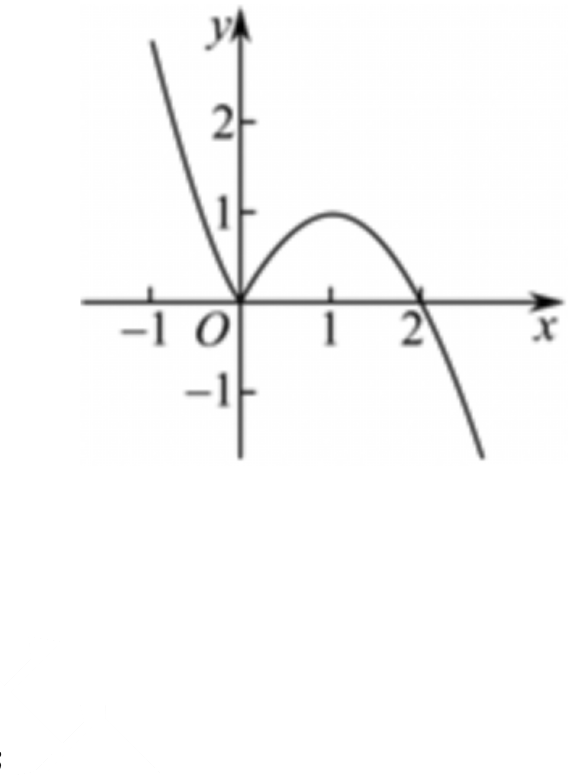
\includegraphics[width=0.20\textwidth]{figures/gao83_q15_graph.png}
\end{center}
\step{由 $[f(x)]^2+af(x)<0$ 得 $[f(x)+a]f(x)<0$，}
\step{当 $a=0$ 时，$[f(x)]^2<0$，不等式无解；}
\step{当 $a>0$ 时，由 $[f(x)+a]f(x)<0$ 得 $-a<f(x)<0$，}
\step{若不等式恰有 $1$ 个整数解，则整数解为 $3$，}
\step{又 $f(3)=-3$，$f(4)=-8$，所以 $-8\leqslant-a<-3$，所以 $3<a\leqslant8$；}
\step{当 $a<0$ 时，由 $[f(x)+a]f(x)<0$ 得 $0<f(x)<-a$，此时有多个解，故舍去；}
\step{综上所述，实数 $a$ 的取值范围为 $(3,8]$. 故选 $C$.}
\solend
\fi

\item 设函数 $f(x)=\begin{cases}\lvert2^x-1\rvert,&x\leqslant2\\ -x+7,&x>2\end{cases}$，若互不相等的实数 $a$、$b$、$c$ 满足 $f(a)=f(b)=f(c)$，
则 $2^a+2^b+2^c$ 的取值范围是\mbox{（\quad）}

\keepwithprev
A. $(8,9)$\qquad B. $(65,129)$\qquad C. $(64,128)$\qquad D. $(66,130)$

\ifanswer
\solbegin
\step{作出函数 $f(x)=\begin{cases}\lvert2^x-1\rvert,&x\leqslant2\\ -x+7,&x>2\end{cases}$ 的图象如图，}
\begin{center}
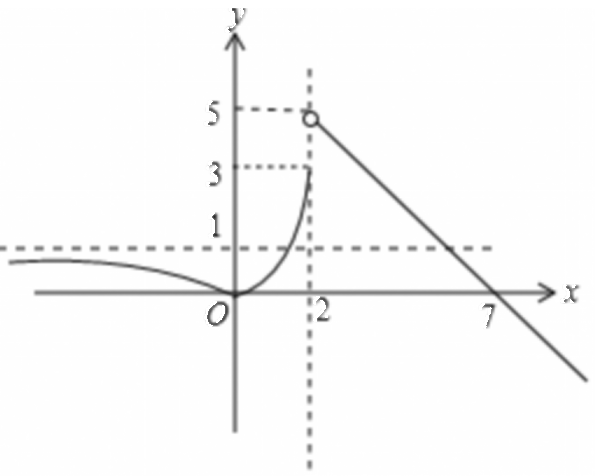
\includegraphics[width=0.22\textwidth]{figures/gao83_q16_graph.png}
\end{center}
\step{不妨设 $a<b<c$，由 $f(a)=f(b)$，得 $1-2^a=2^b-1$，则 $2^a+2^b=2$.}
\step{由 $f(-c)-c+6\in(0,1)$，得 $c\in(6,7)$，则 $64<2^c<128$，}
\step{所以 $66<2^a+2^b+2^c<130$，即 $2^a+2^b+2^c$ 的取值范围是 $(66,130)$. 故选 $D$.}
\solend
\fi

\end{enumerate}

\bigsec{三、解答题}

\begin{enumerate}
\setcounter{enumi}{16}

\item 已知幂函数 $f(x)$ 与一次函数 $g(x)$ 的图象都经过点 $(4,2)$，且 $f(9)=g(5)$.

（1）求 $f(x)$ 与 $g(x)$ 的解析式；

（2）求函数 $h(x)=g(x)-f(x)$ 在 $[0,4]$ 上的值域.

\ansspace*[8]

\ifanswer
\solbegin
\stepm{（1）}{设 $f(x)=x^\alpha$，$g(x)=kx+b$，则 $4^\alpha=2$，即 $\alpha=\dfrac12$，}
\step{$\begin{cases}4k+b=2\\ 3=5k+b\end{cases}$，则 $k=1$，$b=-2$，所以 $f(x)=\sqrt x$，$g(x)=x-2$；}
\stepm{（2）}{$h(x)=g(x)-f(x)=x-\sqrt x-2$，}
\step{令 $t=\sqrt x$，则 $t\in[0,2]$，原函数可化为 $p(t)=t^2-t-2$，}
\step{当 $t=\dfrac12$ 时，函数取得最小值 $-\dfrac94$，当 $t=2$ 时，函数取得最大值 $0$，}
\step{即函数值域为 $\left[-\dfrac94,0\right]$.}
\solend
\fi

\item 目前某县有 $100$ 万人. 经过 $x$ 年后为 $y$ 万人. 如果年平均增长率是 $1.2\%$. 请回答下列问题：

（1）写出 $y$ 关于 $x$ 的函数解析式.

（2）计算 $10$ 年后该县的人口总数（精确到 $0.1$ 万人）.

（3）计算大约多少年后该县的人口总数将达到 $120$ 万（精确到 $1$ 年）.

\ansspace*[9]

\ifanswer
\solbegin
\stepm{（1）}{当 $x=1$ 时，$y=100+100\times1.2\%=100(1+1.2\%)$，}
\step{当 $x=2$ 时，$y=100(1+1.2\%)+100(1+1.2\%)\times1.2\%=100(1+1.2\%)^2$，}
\step{当 $x=3$ 时，$y=100(1+1.2\%)^2+100(1+1.2\%)^2\times1.2\%=100(1+1.2\%)^3$，}
\step{$\cdots\cdots$}
\step{故 $y$ 关于 $x$ 的函数解析式为 $y=100(1+1.2\%)^x\,(x\in\N^*)$；}
\stepm{（2）}{当 $x=10$ 时，$y=100(1+1.2\%)^{10}=100\times1.012^{10}\approx112.7$，}
\step{故 $10$ 年后该县的人口总数约为 $112.7$ 万人；}
\stepm{（3）}{设 $x$ 年后该县的人口总数将达到 $120$ 万，即 $y=100(1+1.2\%)^x=120$，}
\step{解得 $x=\log_{1.012}\dfrac{120}{100}\approx16$，故大约 $16$ 年后该县的人口总数将达到 $120$ 万.}
\solend
\fi

\item 已知 $a>0$ 且 $a\neq1$，$m>0$，函数 $f(x)=(m^2+m-5)a^x$ 是指数函数，且 $f(2)=4$.

（1）求实数 $m$ 和 $a$ 的值；

（2）$f(2x)-2f(x)+2\geqslant nf(x)$ 对任意 $x\in[-1,2]$ 恒成立，求实数 $n$ 的取值范围；

（3）若关于 $x$ 的方程 $f(2x)-(2k+8)f(x)+2k+7b=0$ 有两个不相等的实数根，且一根
大于 $0$，另一根小于 $0$，其中 $k>0$，求整数 $b$ 的最大值.

\ansspace*[11]

\ifanswer
\solbegin
\stepm{（1）}{因为函数 $f(x)=(m^2+m-5)a^x$ 是指数函数，}
\step{所以 $m^2+m-5=1$，即 $m^2+m-6=0$，解得 $m=2$ 或 $m=-3$，}
\step{又 $m>0$，所以 $m=2$，又 $f(2)=a^2=4$，$a>0$ 且 $a\neq1$，所以 $a=2$；}
\stepm{（2）}{由（1）得 $f(x)=2^x$，}
\step{由题意 $2^{2x}-2\cdot2^x+2\geqslant n2^x$ 对任意 $x\in[-1,2]$ 恒成立，}
\step{所以 $n\leqslant2^x-2+\dfrac2{2^x}$ 对任意 $x\in[-1,2]$ 恒成立，则 $n\leqslant\left(2^x-2+\dfrac2{2^x}\right)_{\min}$，}
\step{记 $g(x)=2^x-2+\dfrac2{2^x}$，$x\in[-1,2]$，}
\step{令 $t=2^x$，因为 $x\in[-1,2]$，所以 $t\in\left[\dfrac12,4\right]$，则 $y=t+\dfrac2t-2$，$t\in\left[\dfrac12,4\right]$，}
\step{函数 $y=t+\dfrac2t-2$ 在 $\left[\dfrac12,\sqrt2\right]$ 上严格减，在 $[\sqrt2,4]$ 上严格增，}
\step{所以 $y=t+\dfrac2t-2$ 的最小值为 $\sqrt2+\dfrac2{\sqrt2}-2=2\sqrt2-2$，}
\step{所以 $n\leqslant2\sqrt2-2$，即实数 $n$ 的取值范围为 $(-\infty,2\sqrt2-2]$；}
\stepm{（3）}{方程 $f(2x)-(2k+8)f(x)+2k+7b=0$，}
\step{即方程 $2^{2x}-(2k+8)2^x+2k+7b=0$，即方程 $(2^x)^2-(2k+8)2^x+2k+7b=0$，}
\step{令 $t=2^x>0$，则方程 $t^2-(2k+8)t+2k+7b=0$，}
\step{因为关于 $x$ 的方程 $f(2x)-(2k+8)f(x)+2k+7b=0$ 的一根大于 $0$，另一根小于 $0$，}
\step{所以关于 $t$ 的方程 $t^2-(2k+8)t+2k+7b=0$ 的一根大于 $1$，另一根大于 $0$ 且小于 $1$，}
\step{记 $h(t)=t^2-(2k+8)t+2k+7b$，}
\step{所以 $\begin{cases}h(1)=1^2-(2k+8)\cdot1+2k+7b<0\\ h(0)=2k+7b>0\\ k>0\end{cases}$，所以 $\begin{cases}b<1\\ b>-\dfrac27k\\ k>0\end{cases}$，}
\step{所以整数 $b$ 的最大值为 $0$.}
\solend
\fi

\item 已知幂函数 $f(x)=(p^2-3p+3)x^{p^2-\frac32p-\frac12}$ 满足 $f(2)<f(4)$.

（1）求函数 $f(x)$ 的解析式；

（2）若函数 $g(x)=f^2(x)+mf(x)$，$x\in[1,9]$，是否存在实数 $m$ 使得 $g(x)$ 的最小值为 $0$？
若存在，求出 $m$ 的值；若不存在，说明理由.

（3）若函数 $h(x)=n-f(x+3)$，是否存在实数 $a$、$b\,(a<b)$，使函数 $h(x)$ 在 $[a,b]$ 上的
值域为 $[a,b]$？若存在，求出实数 $n$ 的取值范围；若不存在，说明理由.

\ansspace*[12]

\ifanswer
\solbegin
\stepm{（1）}{因为 $f(x)$ 是幂函数，所以 $p^2-3p+3=1$，解得 $p=1$ 或 $p=2$，}
\step{当 $p=1$ 时，$f(x)=\dfrac1x$，不满足 $f(2)<f(4)$.}
\step{当 $p=2$ 时，$f(x)=\sqrt x$，满足 $f(2)<f(4)$.}
\step{故 $p=2$，函数 $f(x)$ 的解析式为 $f(x)=\sqrt x$；}
\stepm{（2）}{由函数 $g(x)=f^2(x)+mf(x)$，即 $g(x)=(\sqrt x)^2+m\sqrt x$，}
\step{令 $t=\sqrt x$，因为 $x\in[1,9]$，所以 $t\in[1,3]$，}
\step{记 $k(x)=t^2+mt$，其对称轴 $t=-\dfrac m2$，}
\step{①当 $-\dfrac m2\leqslant1$，即 $m\geqslant-2$ 时，则 $k(x)_{\min}=k(1)=1+m=0$，解得 $m=-1$；}
\step{②当 $1<-\dfrac m2<3$ 时，即 $-6<m<-2$，则 $k(x)_{\min}=k\left(-\dfrac m2\right)=-\dfrac{m^2}4=0$，}
\step{解得 $m=0$，不满足，舍去；}
\step{③当 $-\dfrac m2\geqslant3$ 时，即 $m\leqslant-6$ 时，则 $k(x)_{\min}=k(3)=3m+9=0$，解得 $m=-3$，}
\step{不满足，舍去；}
\step{综上所述，存在 $m=-1$ 使得 $g(x)$ 的最小值为 $0$；}
\stepm{（3）}{由函数 $h(x)=n-f(x+3)=n-\sqrt{x+3}$ 在定义域内为严格减函数，}
\step{若存在实数 $a$、$b\,(a<b)$，使函数 $h(x)$ 在 $[a,b]$ 上的值域为 $[a,b]$，}
\step{则 $h(x)=\begin{cases}n-\sqrt{a+3}=b\text{ ①}\\ n-\sqrt{b+3}=a\text{ ②}\end{cases}$，}
\step{两式相减得 $\sqrt{a+3}-\sqrt{b+3}=a-b=(a+3)-(b+3)$，}
\step{所以 $\sqrt{a+3}+\sqrt{b+3}=1$ ③，}
\step{将③代入②得 $n=a+\sqrt{b+3}=a+1-\sqrt{a+3}$，}
\step{令 $t=\sqrt{a+3}$，因为 $a<b$，所以 $0\leqslant t<\dfrac12$，得 $n=t^2-t-2=\left(t-\dfrac12\right)^2-\dfrac94$，}
\step{故实数 $n$ 的取值范围为 $\left(-\dfrac94,-2\right]$.}
\solend
\fi

\item 定理（三角不等式），对于任意的 $a$、$b\in\R$，恒有 $\bigl\lvert\lvert a\rvert-\lvert b\rvert\bigr\rvert\leqslant\lvert a\pm b\rvert\leqslant\lvert a\rvert+\lvert b\rvert$. 定义：
已知 $n\in\N$ 且 $n\geqslant3$，对于有序数组 $a_1$、$a_2$、$\cdots$、$a_n$，称 $\lvert a_1-a_2\rvert+\lvert a_2-a_3\rvert+\cdots+\lvert a_{n-1}-a_n\rvert$
为有序数组 $a_1$、$a_2$、$\cdots$、$a_n$ 的波动距离，记作 $f(a_1,a_2,\cdots,a_n)$，即
$f(a_1,a_2,\cdots,a_n)=\lvert a_1-a_2\rvert+\lvert a_2-a_3\rvert+\cdots+\lvert a_{n-1}-a_n\rvert$，请根据上述信息解决以下几个问题：

（1）求函数 $y=\lvert x-2\rvert+\lvert x-4\rvert$ 的最小值，并指出函数取到最小值时 $x$ 的取值范围；

（2）①求有序数组 $2$、$5$、$3$、$4$ 的波动距离 $f(2,5,3,4)$；

②求证：若 $a$、$b$、$c$、$d\in\R$ 且 $a<b<c$，则 $f(a,b,c,d)\leqslant f(a,c,b,d)$；

（3）同理可证得命题“若 $a$、$b$、$c$、$d\in\R$ 且 $c<b<a$ 时，$f(a,b,c,d)\leqslant f(a,c,b,d)$”也
是真命题（注：该命题无需证明，需要时可直接使用）.

设两两不相等的四个实数 $a_1$、$a_2$、$a_3$、$a_4\in\{3^1,3^2,3^3,3^4\}$，求有序数组 $a_1$、$a_2$、$a_3$、$a_4$ 的
波动距离 $f(a_1,a_2,a_3,a_4)$ 的最大值.

\ansspace*[14]

\ifanswer
\solbegin
\stepm{（1）}{由三角不等式得 $\bigl\lvert\lvert a\rvert-\lvert b\rvert\bigr\rvert\leqslant\lvert a\pm b\rvert\leqslant\lvert a\rvert+\lvert b\rvert$，}
\step{当且仅当 $\lvert a+b\rvert^2=(\lvert a\rvert+\lvert b\rvert)^2$ 时，}
\step{即当 $-ab=\lvert ab\rvert$ 时，即当 $ab\leqslant0$ 时取等号，}
\step{由三角不等式得 $y=\lvert x-2\rvert+\lvert x-4\rvert\geqslant\lvert(x-2)-(x-4)\rvert=2$，}
\step{当且仅当 $(x-2)(x-4)\leqslant0$ 时，即 $2\leqslant x\leqslant4$ 时取等号，}
\step{因此，函数 $y=\lvert x-2\rvert+\lvert x-4\rvert$ 的最小值为 $2$，此时 $x$ 的取值范围是 $[2,4]$.}
\stepm{（2）}{①由题中定义得 $f(2,5,3,4)=\lvert2-5\rvert+\lvert5-3\rvert+\lvert3-4\rvert=6$；}
\step{②$f(a,b,c,d)-f(a,c,b,d)=\lvert a-b\rvert+\lvert c-d\rvert-\lvert a-c\rvert-\lvert b-d\rvert$，}
\step{因为 $a<b<c$，所以 $\lvert a-b\rvert-\lvert a-c\rvert=-\lvert b-c\rvert$，$\lvert c-d\rvert-\lvert b-d\rvert\leqslant\lvert b-c\rvert$，}
\step{所以 $f(a,b,c,d)-f(a,c,b,d)\leqslant0$，即 $f(a,b,c,d)\leqslant f(a,c,b,d)$，}
\stepm{（3）}{$f(a,b,c,d)=\lvert a-b\rvert+\lvert b-c\rvert+\lvert c-d\rvert$}
\step{$=\lvert d-c\rvert+\lvert c-b\rvert+\lvert b-a\rvert=f(d,c,b,a)$，}
\step{当 $f(a_1,a_2,a_3,a_4)$ 取得最大值时，$a_2=\max\{a_1,a_2,a_3\}$ 或 $a_2=\min\{a_1,a_2,a_3\}$，}
\step{同理 $a_3=\max\{a_2,a_3,a_4\}$ 或 $a_3=\min\{a_2,a_3,a_4\}$，}
\step{若 $a_2=\max\{a_1,a_2,a_3\}$，则 $a_2>a_3$，所以 $a_3=\min\{a_2,a_3,a_4\}$，}
\step{故 $f(a_1,a_2,a_3,a_4)=\lvert a_1-a_2\rvert+\lvert a_2-a_3\rvert+\lvert a_3-a_4\rvert=a_2-a_1+a_2-a_3+a_4-a_3$}
\step{$=2a_2+a_4-2a_3-a_1\leqslant2\times3^4+3^3-2\times3^1-3^2=174$，}
\step{当且仅当 $a_1=3^2$，$a_2=3^4$，$a_3=3^1$，$a_4=3^3$ 时取等号，}
\step{所以 $f(3^2,3^4,3^1,3^3)$ 为 $f(a_1,a_2,a_3,a_4)$ 的最大值，}
\step{若 $a_2=\min\{a_1,a_2,a_3\}$，则 $a_2<a_3$，所以 $a_3=\max\{a_2,a_3,a_4\}$，}
\step{同理可得 $f(3^3,3^4,3^1,3^2)$ 为 $f(a_1,a_2,a_3,a_4)$ 的最大值，}
\step{综上所述，$f(a_1,a_2,a_3,a_4)$ 的最大值为 $174$.}
\solend
\fi

\end{enumerate}

\end{document}
"
% 紧凑版：xelatex "\def\iscompact{1}% 高一83_交附闵行_周末作业10.23.tex
%   —— 高一上数学“2026-2027 年交附闵行高一上周末作业 10.23”（讲评版）
% 试卷版：xelatex 高一83_交附闵行_周末作业10.23.tex
% 答案版：xelatex "\def\isanswer{1}% 高一83_交附闵行_周末作业10.23.tex
%   —— 高一上数学“2026-2027 年交附闵行高一上周末作业 10.23”（讲评版）
% 试卷版：xelatex 高一83_交附闵行_周末作业10.23.tex
% 答案版：xelatex "\def\isanswer{1}\input{高一83_交附闵行_周末作业10.23.tex}"
% 紧凑版：xelatex "\def\iscompact{1}\input{高一83_交附闵行_周末作业10.23.tex}"
%
% 原始材料：微信公众号“魔都数学加油站”文章，连载“27学年高一83”；
% 原文标题“27学年高一83——2026-2027年上海市交附闵行高一上周末作业10.23”；
% 原文链接：https://mp.weixin.qq.com/s/t5AfTwQXg4Sj4i_Dl5rgXA。
% 页面标注发布时间 2026-10-26 20:15（上海）。
% 正文为 12 张 PNG 页（`原图/高一83_交附闵行_周末作业10.23/01..12.png`），
% 尺寸混排（第 1—8 页为 4762×6735，第 9—12 页为 2560×3620），均按页序读取。
%
% 篇幅与题号：原卷自第 3 题起编号（第 1、2 题不在原文内）。填空题 3—12（10 题）、
% 选择题 13—16（4 题）、解答题 17—21（5 题），共 19 题。
%
% 讲评版：19 题全部印【解析】，本稿不另提 \ans{}；选择题答案在解析末句“故选 C／B／C／D”。
%
% 副标题：原卷未印副标题。本稿按内容标作“函数与导数”（本卷考幂函数、指数函数、
% 对数与函数应用，属“函数与导数”模块；副标题只用知识模块名，见 README 说明）。
%
% 与原卷的排版差异：
%   ① 原卷每题下直接印【解析】，本稿按全稿惯例将解析置于答案版；
%   ② 原卷未印副标题，本稿补出；填空横线统一排 \blankline[4.4em]；
%   ③ 原卷数集记号排斜体 $R$、$Z$、$N$，本稿按全稿惯例改用 $\R$、$\Z$、$\N$；
%   ④ 第 17—21 题的子问用行内“（1）（2）（3）”段，解析中的子问标号用 \stepm；
%   ⑤ 解答题按惯例加 \ansspace；选择题括号排 \mbox{（\quad）}；
%   ⑥ 第 15、16 题解析各有一幅函数图象，裁自原图（第 6 页）后去粉色水印、转灰度，
%      仅答案版出。
%
% 行数核对：逐题数 \step/\stepm 条数，合计 145 条（Q3：1；Q4：1；Q5：4；Q6：5；
% Q7：2；Q8：7；Q9：10；Q10：5；Q11：6；Q12：8；Q13：3；Q14：4；Q15：8；
% Q16：4；Q17：6；Q18：9；Q19：19；Q20：21；Q21：22）。原卷解析的换行
% 按语意合并，未逐行强拆。
%
\documentclass[a4paper,11pt]{article}
\usepackage{common}

\begin{document}

\examtitlest[4]{2026--2027 年交附闵行高一上周末作业 10.23}{函数与导数}

\bigsec{一、填空题}

\begin{enumerate}
\setcounter{enumi}{2}

\item 已知 $10^a=2$，$10^b=5$，则 $10^{3a-2b}$ 的值为\blankline[4.4em].

\ifanswer
\solbegin
\step{$10^{3a-2b}=\dfrac{10^{3a}}{10^{2b}}=\dfrac{(10^a)^3}{(10^b)^2}=\dfrac{2^3}{5^2}=\dfrac8{25}$.}
\solend
\fi

\item 根式 $a\sqrt{-a}$ 化成分数指数幂是\blankline[4.4em].

\ifanswer
\solbegin
\step{$a\sqrt{-a}=a(-a)^{\frac12}=-(-a)(-a)^{\frac12}=-(-a)^{\frac32}$.}
\solend
\fi

\item 已知数列 $\{a_n\}$ 的通项公式为 $a_n=\left(\dfrac49\right)^{n-1}-\left(\dfrac23\right)^{n-1}$，在下列说法中：①有最大项；
②有最小项；③没有最大项；④没有最小项. 正确的是\blankline[3.6em]（填序号）.

\ifanswer
\solbegin
\step{令 $t=\left(\dfrac23\right)^{n-1}$，则 $t\in\left\{1,\dfrac23,\dfrac49,\dfrac8{27},\cdots\right\}\subset(0,1]$，$t$ 是关于 $n$ 的减函数，}
\step{则 $a_n=t^2-t=\left(t-\dfrac12\right)^2-\dfrac14$，}
\step{所以当 $t=1$ 即 $n=1$ 时 $a_n$ 取得最大为 $0$，当 $t=\dfrac49$ 即 $n=3$ 时 $a_n$ 取得最小为 $-\dfrac{20}{81}$，}
\step{所以 $a_n$ 既有最大项又有最小项，故①和②正确.}
\solend
\fi

\item 已知 $f(x)=\mathrm{e}^{x-\frac12}-\mathrm{e}^{-x+\frac12}+\dfrac{4x}{2x-1}$，则
$f\left(\dfrac1{2020}\right)+f\left(\dfrac2{2020}\right)+f\left(\dfrac3{2020}\right)+\cdots+f\left(\dfrac{1009}{2020}\right)+f\left(\dfrac{1011}{2020}\right)+\cdots+f\left(\dfrac{2019}{2020}\right)$ 的
值为\blankline[4.4em].

\ifanswer
\solbegin
\step{因为 $f(x)+f(1-x)=\mathrm{e}^{x-\frac12}-\mathrm{e}^{-x+\frac12}+\dfrac{4x}{2x-1}+\mathrm{e}^{(1-x)-\frac12}-\mathrm{e}^{-(1-x)+\frac12}+\dfrac{4(1-x)}{2(1-x)-1}$}
\step{$=\dfrac{4x}{2x-1}+\dfrac{4-4x}{1-2x}=\dfrac{4(2x-1)}{2x-1}=4$，}
\step{记 $S=f\left(\dfrac1{2020}\right)+f\left(\dfrac2{2020}\right)+\cdots+f\left(\dfrac{2019}{2020}\right)$，}
\step{又 $S=f\left(\dfrac{2019}{2020}\right)+f\left(\dfrac{2018}{2020}\right)+\cdots+f\left(\dfrac2{2020}\right)+f\left(\dfrac1{2020}\right)$，}
\step{对齐相加得 $2S=2018\times4$，所以 $S=4036$.}
\solend
\fi

\item 不等式 $2^{x^2-2x-3}<\left(\dfrac12\right)^{3(x-1)}$ 的解集为\blankline[4.4em].

\ifanswer
\solbegin
\step{由 $2^{x^2-2x-3}<\left(\dfrac12\right)^{3(x-1)}$ 得 $x^2-2x-3<-3(x-1)$，即 $x^2+x-6<0$，}
\step{故解集为 $(-3,2)$.}
\solend
\fi

\item 函数 $f(x)=x^{\ln5}+x^{\ln12}-13^{\ln x}$ 的零点是\blankline[4.4em]. 附：$a^{\log_bc}=c^{\log_ba}$
（$a>0$，$b>0$，$c>0$，$b\neq1$）.

\ifanswer
\solbegin
\step{函数 $f(x)=x^{\ln5}+x^{\ln12}-13^{\ln x}$，}
\step{若 $f(x)=x^{\ln5}+x^{\ln12}-13^{\ln x}=0$，变形得 $x^{\ln5}+x^{\ln12}=13^{\ln x}$，}
\step{又 $a^{\log_bc}=c^{\log_ba}$（$a>0$，$b>0$，$c>0$，$b\neq1$），得 $5^{\ln x}+12^{\ln x}=13^{\ln x}$，}
\step{令 $g(t)=\left(\dfrac5{13}\right)^t+\left(\dfrac{12}{13}\right)^t-1$，易得 $g(t)$ 严格减，所以 $g(t)=0$ 至多有一解，}
\step{即 $\left(\dfrac5{13}\right)^t+\left(\dfrac{12}{13}\right)^t-1=0$ 至多有一解，变形得方程 $5^t+12^t=13^t$ 至多有一解，}
\step{易得 $t=2$ 时，有 $5^2+12^2=13^2$ 成立，则方程 $5^t+12^t=13^t$ 有唯一解 $t=2$，}
\step{即 $\ln x=2$，解得 $x=\mathrm{e}^2$，即函数 $f(x)$ 的零点为 $\mathrm{e}^2$.}
\solend
\fi

\item 已知幂函数 $f(x)=(m^2-2m-2)x^{m^2+m-2}$ 在 $(0,+\infty)$ 上是严格减函数，则不等式
$f(x-1)<f(3-2x)$ 的解集为\blankline[4.4em].

\ifanswer
\solbegin
\step{因为 $f(x)$ 为幂函数，所以 $m^2-2m-2=1$，解得 $m=-1$ 或 $m=3$；}
\step{当 $m=3$ 时，$f(x)=x^{10}$ 在 $(0,+\infty)$ 上严格增，不合题意；}
\step{当 $m=-1$ 时，$f(x)=x^{-2}$ 在 $(0,+\infty)$ 上严格减，符合题意；}
\step{综上所述，$m=-1$；}
\step{因为 $f(x)=x^{-2}$ 的定义域为 $(-\infty,0)\cup(0,+\infty)$，$f(-x)=(-x)^{-2}=x^{-2}=f(x)$，}
\step{所以 $f(x)$ 为定义在 $(-\infty,0)\cup(0,+\infty)$ 上的偶函数，}
\step{故 $f(x-1)=f(\lvert x-1\rvert)$，$f(3-2x)=f(\lvert3-2x\rvert)$，}
\step{$f(x-1)<f(3-2x)\Rightarrow f(\lvert x-1\rvert)<f(\lvert3-2x\rvert)\Rightarrow\lvert x-1\rvert>\lvert3-2x\rvert$}
\step{且 $\lvert x-1\rvert\neq0$，$\lvert3-2x\rvert\neq0$，解得 $\dfrac43<x<\dfrac32$ 或 $\dfrac32<x<2$，}
\step{所以 $f(x-1)<f(3-2x)$ 的解集为 $\left(\dfrac43,\dfrac32\right)\cup\left(\dfrac32,2\right)$.}
\solend
\fi

\item 若实数 $x_1$、$x_2$ 满足 $\mathrm{e}^{x_1}+x_1-3=0$，$x_2\ln x_2+3x_2-1=0$，则 $\dfrac{x_1x_2+1}{x_2}$ 的值为\blankline[4.4em].

\ifanswer
\solbegin
\step{易得 $x_2>0$，则 $\ln x_2+3-\dfrac1{x_2}=0$，即 $\mathrm{e}^{-\ln x_2}+(-\ln x_2)-3=0$.}
\step{设 $f(x)=\mathrm{e}^x+x-3$，则函数 $f(x)$ 在 $(-\infty,+\infty)$ 上严格增.}
\step{由 $\mathrm{e}^{x_1}+x_1-3=0$，$\mathrm{e}^{-\ln x_2}+(-\ln x_2)-3=0$，得 $f(x_1)=0$，$f(-\ln x_2)=0$，}
\step{所以 $f(x_1)=f(-\ln x_2)$，得 $x_1=-\ln x_2$，即 $\ln x_2=-x_1$，所以 $x_2=\mathrm{e}^{-x_1}$，得 $\dfrac1{x_2}=\mathrm{e}^{x_1}$.}
\step{因为 $\mathrm{e}^{x_1}+x_1-3=0$，所以 $\mathrm{e}^{x_1}+x_1=3$，所以 $\dfrac{x_1x_2+1}{x_2}=x_1+\dfrac1{x_2}=\mathrm{e}^{x_1}+x_1=3$.}
\solend
\fi

\item 已知 $\alpha$、$\beta$ 是方程 $9^x-2m\cdot3^x+m^2-1=0$ 的两个根，若 $\alpha+\beta=1$，则 $\alpha\beta=\blankline[4.4em]$.

\ifanswer
\solbegin
\step{由题意得方程 $9^x-2m\cdot3^x+m^2-1=0$ 有两个根，}
\step{则方程 $t^2-2mt+m^2-1=0$ 有二正根，则 $\begin{cases}\Delta=4m^2-4(m^2-1)\geqslant0\\ 2m>0\\ m^2-1>0\end{cases}$，解得 $m>1$，}
\step{又 $\alpha$、$\beta$ 是方程 $9^x-2m\cdot3^x+m^2-1=0$ 的两个根，则 $3^\alpha\times3^\beta=m^2-1$，}
\step{又 $\alpha+\beta=1$，则 $m^2-1=3^{\alpha+\beta}=3$，解得 $m=2$ 或 $m=-2$（舍），}
\step{则 $3^\alpha+3^\beta=2m=4$，又 $\alpha=1-\beta$，则 $3^{1-\beta}+3^\beta=4$，解得 $\beta=0$ 或 $\beta=1$，}
\step{则 $\begin{cases}\alpha=1\\ \beta=0\end{cases}$ 或 $\begin{cases}\alpha=0\\ \beta=1\end{cases}$，则 $\alpha\beta=0$.}
\solend
\fi

\item 已知实数 $a,b,c\in(1,+\infty)$，满足 $a^{\log_ba}\cdot b^{\log_cb}\cdot c^{\log_ac}=100$，则 $abc$ 的最大值为\blankline[4.4em].

\ifanswer
\solbegin
\step{由换底公式得 $\log_ba=\dfrac{\ln a}{\ln b}$，$\log_cb=\dfrac{\ln b}{\ln c}$，$\log_ac=\dfrac{\ln c}{\ln a}$，}
\step{设 $X=\ln a$，$Y=\ln b$，$Z=\ln c$，得 $a=\mathrm{e}^X$，$b=\mathrm{e}^Y$，$c=\mathrm{e}^Z$，}
\step{代入得 $a^{\log_ba}\cdot b^{\log_cb}\cdot c^{\log_ac}=a^{\frac{\ln a}{\ln b}}\cdot b^{\frac{\ln b}{\ln c}}\cdot c^{\frac{\ln c}{\ln a}}=(\mathrm{e}^X)^{\frac XY}\cdot(\mathrm{e}^Y)^{\frac YZ}\cdot(\mathrm{e}^Z)^{\frac ZX}=100$，}
\step{即 $\mathrm{e}^{\frac{X^2}Y+\frac{Y^2}Z+\frac{Z^2}X}=100$，两边取对数得 $\dfrac{X^2}Y+\dfrac{Y^2}Z+\dfrac{Z^2}X=\ln100$.}
\step{由 $a,b,c\in(1,+\infty)$，得 $X>0$，$Y>0$，$Z>0$，}
\step{由柯西不等式，得 $\left(\dfrac{X^2}Y+\dfrac{Y^2}Z+\dfrac{Z^2}X\right)(X+Y+Z)\geqslant(X+Y+Z)^2$，}
\step{即 $X+Y+Z\leqslant\dfrac{X^2}Y+\dfrac{Y^2}Z+\dfrac{Z^2}X=\ln100$，当且仅当 $X=Y=Z$ 时取等号，}
\step{因此 $(X+Y+Z)_{\max}=\ln100$，所以 $(abc)_{\max}=\mathrm{e}^{(X+Y+Z)_{\max}}=\mathrm{e}^{\ln100}=100$.}
\solend
\fi

\end{enumerate}

\bigsec{二、选择题}

\begin{enumerate}
\setcounter{enumi}{12}

\item 已知集合 $A=\{x\mid x=2k,k\in\Z\}$，$B=\{x\mid x=4k+2,\,k\in\Z\}$，则 $A\cup B=\mbox{（\quad）}$

\keepwithprev
A. $B$\qquad B. $\R$\qquad C. $A$\qquad D. 以上都不是

\ifanswer
\solbegin
\step{$B=\{x\mid x=4k+2,k\in\Z\}=\{x\mid x=2(2k+1),k\in\Z\}$，它表示奇数的 $2$ 倍组成的集合，}
\step{$A=\{x\mid x=2k,k\in\Z\}$，即集合 $A$ 是整数的 $2$ 倍组成的集合，}
\step{则 $B\subseteq A$，则 $A\cup B=A$. 故选 $C$.}
\solend
\fi

\item 教室通风的目的是通过空气的流动，排出室内的污浊空气和致病微生物，降低室内二氧化碳和致病微生物的浓度，送进室外的新鲜空气. 按照国家标准，教室内空气中二氧化碳日平均最高容许浓度应小于等于 $0.1\%$. 经测定，刚下课时，空气中含有 $0.2\%$ 的二氧化碳，若开窗通风后教室内二氧化碳的浓度为 $y\%$，且 $y$ 随时间 $t$（单位：分钟）的变化规律可以用函数 $y=0.05+\lambda\mathrm{e}^{-\frac t{12}}\,(\lambda\in\R)$ 描述，则该教室内的二氧化碳浓度达到国家标准至少需要的时间为\mbox{（\quad）}

\keepwithprev
A. $10$ 分钟\qquad B. $14$ 分钟\qquad C. $15$ 分钟\qquad D. $20$ 分钟

\ifanswer
\solbegin
\step{由题意得，当 $t=0$ 时，$y=0.2$，即 $0.05+\lambda\mathrm{e}^0=0.2$，解得 $\lambda=0.15$，}
\step{所以 $y=0.05+0.15\mathrm{e}^{-\frac t{12}}$，由题意得 $0.05+0.15\mathrm{e}^{-\frac t{12}}\leqslant0.1$，即 $\mathrm{e}^{-\frac t{12}}\leqslant\dfrac13$，}
\step{两边取对数得 $-\dfrac t{12}\leqslant-\ln3$，所以 $t\geqslant12\ln3\approx13.2$，}
\step{所以该教室内的二氧化碳浓度达到国家标准至少需要的时间为 $14$ 分钟. 故选 $B$.}
\solend
\fi

\item 已知函数 $f(x)=\begin{cases}-x^2+2x,&x\geqslant0\\ x^2-2x,&x<0\end{cases}$，若关于 $x$ 的不等式 $[f(x)]^2+af(x)<0$ 恰有 $1$ 个整数
解，则实数 $a$ 的最大值为\mbox{（\quad）}

\keepwithprev
A. $-2$\qquad B. $3$\qquad C. $8$\qquad D. $9$

\ifanswer
\solbegin
\step{作出 $f(x)$ 的图象，如图所示：}
\begin{center}
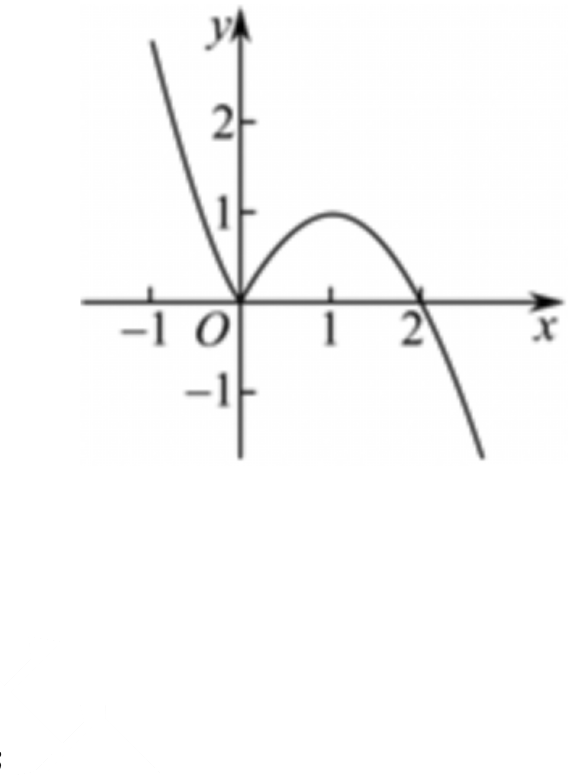
\includegraphics[width=0.20\textwidth]{figures/gao83_q15_graph.png}
\end{center}
\step{由 $[f(x)]^2+af(x)<0$ 得 $[f(x)+a]f(x)<0$，}
\step{当 $a=0$ 时，$[f(x)]^2<0$，不等式无解；}
\step{当 $a>0$ 时，由 $[f(x)+a]f(x)<0$ 得 $-a<f(x)<0$，}
\step{若不等式恰有 $1$ 个整数解，则整数解为 $3$，}
\step{又 $f(3)=-3$，$f(4)=-8$，所以 $-8\leqslant-a<-3$，所以 $3<a\leqslant8$；}
\step{当 $a<0$ 时，由 $[f(x)+a]f(x)<0$ 得 $0<f(x)<-a$，此时有多个解，故舍去；}
\step{综上所述，实数 $a$ 的取值范围为 $(3,8]$. 故选 $C$.}
\solend
\fi

\item 设函数 $f(x)=\begin{cases}\lvert2^x-1\rvert,&x\leqslant2\\ -x+7,&x>2\end{cases}$，若互不相等的实数 $a$、$b$、$c$ 满足 $f(a)=f(b)=f(c)$，
则 $2^a+2^b+2^c$ 的取值范围是\mbox{（\quad）}

\keepwithprev
A. $(8,9)$\qquad B. $(65,129)$\qquad C. $(64,128)$\qquad D. $(66,130)$

\ifanswer
\solbegin
\step{作出函数 $f(x)=\begin{cases}\lvert2^x-1\rvert,&x\leqslant2\\ -x+7,&x>2\end{cases}$ 的图象如图，}
\begin{center}
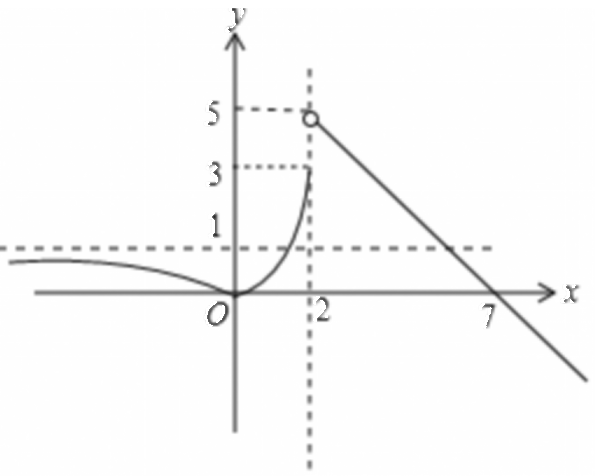
\includegraphics[width=0.22\textwidth]{figures/gao83_q16_graph.png}
\end{center}
\step{不妨设 $a<b<c$，由 $f(a)=f(b)$，得 $1-2^a=2^b-1$，则 $2^a+2^b=2$.}
\step{由 $f(-c)-c+6\in(0,1)$，得 $c\in(6,7)$，则 $64<2^c<128$，}
\step{所以 $66<2^a+2^b+2^c<130$，即 $2^a+2^b+2^c$ 的取值范围是 $(66,130)$. 故选 $D$.}
\solend
\fi

\end{enumerate}

\bigsec{三、解答题}

\begin{enumerate}
\setcounter{enumi}{16}

\item 已知幂函数 $f(x)$ 与一次函数 $g(x)$ 的图象都经过点 $(4,2)$，且 $f(9)=g(5)$.

（1）求 $f(x)$ 与 $g(x)$ 的解析式；

（2）求函数 $h(x)=g(x)-f(x)$ 在 $[0,4]$ 上的值域.

\ansspace*[8]

\ifanswer
\solbegin
\stepm{（1）}{设 $f(x)=x^\alpha$，$g(x)=kx+b$，则 $4^\alpha=2$，即 $\alpha=\dfrac12$，}
\step{$\begin{cases}4k+b=2\\ 3=5k+b\end{cases}$，则 $k=1$，$b=-2$，所以 $f(x)=\sqrt x$，$g(x)=x-2$；}
\stepm{（2）}{$h(x)=g(x)-f(x)=x-\sqrt x-2$，}
\step{令 $t=\sqrt x$，则 $t\in[0,2]$，原函数可化为 $p(t)=t^2-t-2$，}
\step{当 $t=\dfrac12$ 时，函数取得最小值 $-\dfrac94$，当 $t=2$ 时，函数取得最大值 $0$，}
\step{即函数值域为 $\left[-\dfrac94,0\right]$.}
\solend
\fi

\item 目前某县有 $100$ 万人. 经过 $x$ 年后为 $y$ 万人. 如果年平均增长率是 $1.2\%$. 请回答下列问题：

（1）写出 $y$ 关于 $x$ 的函数解析式.

（2）计算 $10$ 年后该县的人口总数（精确到 $0.1$ 万人）.

（3）计算大约多少年后该县的人口总数将达到 $120$ 万（精确到 $1$ 年）.

\ansspace*[9]

\ifanswer
\solbegin
\stepm{（1）}{当 $x=1$ 时，$y=100+100\times1.2\%=100(1+1.2\%)$，}
\step{当 $x=2$ 时，$y=100(1+1.2\%)+100(1+1.2\%)\times1.2\%=100(1+1.2\%)^2$，}
\step{当 $x=3$ 时，$y=100(1+1.2\%)^2+100(1+1.2\%)^2\times1.2\%=100(1+1.2\%)^3$，}
\step{$\cdots\cdots$}
\step{故 $y$ 关于 $x$ 的函数解析式为 $y=100(1+1.2\%)^x\,(x\in\N^*)$；}
\stepm{（2）}{当 $x=10$ 时，$y=100(1+1.2\%)^{10}=100\times1.012^{10}\approx112.7$，}
\step{故 $10$ 年后该县的人口总数约为 $112.7$ 万人；}
\stepm{（3）}{设 $x$ 年后该县的人口总数将达到 $120$ 万，即 $y=100(1+1.2\%)^x=120$，}
\step{解得 $x=\log_{1.012}\dfrac{120}{100}\approx16$，故大约 $16$ 年后该县的人口总数将达到 $120$ 万.}
\solend
\fi

\item 已知 $a>0$ 且 $a\neq1$，$m>0$，函数 $f(x)=(m^2+m-5)a^x$ 是指数函数，且 $f(2)=4$.

（1）求实数 $m$ 和 $a$ 的值；

（2）$f(2x)-2f(x)+2\geqslant nf(x)$ 对任意 $x\in[-1,2]$ 恒成立，求实数 $n$ 的取值范围；

（3）若关于 $x$ 的方程 $f(2x)-(2k+8)f(x)+2k+7b=0$ 有两个不相等的实数根，且一根
大于 $0$，另一根小于 $0$，其中 $k>0$，求整数 $b$ 的最大值.

\ansspace*[11]

\ifanswer
\solbegin
\stepm{（1）}{因为函数 $f(x)=(m^2+m-5)a^x$ 是指数函数，}
\step{所以 $m^2+m-5=1$，即 $m^2+m-6=0$，解得 $m=2$ 或 $m=-3$，}
\step{又 $m>0$，所以 $m=2$，又 $f(2)=a^2=4$，$a>0$ 且 $a\neq1$，所以 $a=2$；}
\stepm{（2）}{由（1）得 $f(x)=2^x$，}
\step{由题意 $2^{2x}-2\cdot2^x+2\geqslant n2^x$ 对任意 $x\in[-1,2]$ 恒成立，}
\step{所以 $n\leqslant2^x-2+\dfrac2{2^x}$ 对任意 $x\in[-1,2]$ 恒成立，则 $n\leqslant\left(2^x-2+\dfrac2{2^x}\right)_{\min}$，}
\step{记 $g(x)=2^x-2+\dfrac2{2^x}$，$x\in[-1,2]$，}
\step{令 $t=2^x$，因为 $x\in[-1,2]$，所以 $t\in\left[\dfrac12,4\right]$，则 $y=t+\dfrac2t-2$，$t\in\left[\dfrac12,4\right]$，}
\step{函数 $y=t+\dfrac2t-2$ 在 $\left[\dfrac12,\sqrt2\right]$ 上严格减，在 $[\sqrt2,4]$ 上严格增，}
\step{所以 $y=t+\dfrac2t-2$ 的最小值为 $\sqrt2+\dfrac2{\sqrt2}-2=2\sqrt2-2$，}
\step{所以 $n\leqslant2\sqrt2-2$，即实数 $n$ 的取值范围为 $(-\infty,2\sqrt2-2]$；}
\stepm{（3）}{方程 $f(2x)-(2k+8)f(x)+2k+7b=0$，}
\step{即方程 $2^{2x}-(2k+8)2^x+2k+7b=0$，即方程 $(2^x)^2-(2k+8)2^x+2k+7b=0$，}
\step{令 $t=2^x>0$，则方程 $t^2-(2k+8)t+2k+7b=0$，}
\step{因为关于 $x$ 的方程 $f(2x)-(2k+8)f(x)+2k+7b=0$ 的一根大于 $0$，另一根小于 $0$，}
\step{所以关于 $t$ 的方程 $t^2-(2k+8)t+2k+7b=0$ 的一根大于 $1$，另一根大于 $0$ 且小于 $1$，}
\step{记 $h(t)=t^2-(2k+8)t+2k+7b$，}
\step{所以 $\begin{cases}h(1)=1^2-(2k+8)\cdot1+2k+7b<0\\ h(0)=2k+7b>0\\ k>0\end{cases}$，所以 $\begin{cases}b<1\\ b>-\dfrac27k\\ k>0\end{cases}$，}
\step{所以整数 $b$ 的最大值为 $0$.}
\solend
\fi

\item 已知幂函数 $f(x)=(p^2-3p+3)x^{p^2-\frac32p-\frac12}$ 满足 $f(2)<f(4)$.

（1）求函数 $f(x)$ 的解析式；

（2）若函数 $g(x)=f^2(x)+mf(x)$，$x\in[1,9]$，是否存在实数 $m$ 使得 $g(x)$ 的最小值为 $0$？
若存在，求出 $m$ 的值；若不存在，说明理由.

（3）若函数 $h(x)=n-f(x+3)$，是否存在实数 $a$、$b\,(a<b)$，使函数 $h(x)$ 在 $[a,b]$ 上的
值域为 $[a,b]$？若存在，求出实数 $n$ 的取值范围；若不存在，说明理由.

\ansspace*[12]

\ifanswer
\solbegin
\stepm{（1）}{因为 $f(x)$ 是幂函数，所以 $p^2-3p+3=1$，解得 $p=1$ 或 $p=2$，}
\step{当 $p=1$ 时，$f(x)=\dfrac1x$，不满足 $f(2)<f(4)$.}
\step{当 $p=2$ 时，$f(x)=\sqrt x$，满足 $f(2)<f(4)$.}
\step{故 $p=2$，函数 $f(x)$ 的解析式为 $f(x)=\sqrt x$；}
\stepm{（2）}{由函数 $g(x)=f^2(x)+mf(x)$，即 $g(x)=(\sqrt x)^2+m\sqrt x$，}
\step{令 $t=\sqrt x$，因为 $x\in[1,9]$，所以 $t\in[1,3]$，}
\step{记 $k(x)=t^2+mt$，其对称轴 $t=-\dfrac m2$，}
\step{①当 $-\dfrac m2\leqslant1$，即 $m\geqslant-2$ 时，则 $k(x)_{\min}=k(1)=1+m=0$，解得 $m=-1$；}
\step{②当 $1<-\dfrac m2<3$ 时，即 $-6<m<-2$，则 $k(x)_{\min}=k\left(-\dfrac m2\right)=-\dfrac{m^2}4=0$，}
\step{解得 $m=0$，不满足，舍去；}
\step{③当 $-\dfrac m2\geqslant3$ 时，即 $m\leqslant-6$ 时，则 $k(x)_{\min}=k(3)=3m+9=0$，解得 $m=-3$，}
\step{不满足，舍去；}
\step{综上所述，存在 $m=-1$ 使得 $g(x)$ 的最小值为 $0$；}
\stepm{（3）}{由函数 $h(x)=n-f(x+3)=n-\sqrt{x+3}$ 在定义域内为严格减函数，}
\step{若存在实数 $a$、$b\,(a<b)$，使函数 $h(x)$ 在 $[a,b]$ 上的值域为 $[a,b]$，}
\step{则 $h(x)=\begin{cases}n-\sqrt{a+3}=b\text{ ①}\\ n-\sqrt{b+3}=a\text{ ②}\end{cases}$，}
\step{两式相减得 $\sqrt{a+3}-\sqrt{b+3}=a-b=(a+3)-(b+3)$，}
\step{所以 $\sqrt{a+3}+\sqrt{b+3}=1$ ③，}
\step{将③代入②得 $n=a+\sqrt{b+3}=a+1-\sqrt{a+3}$，}
\step{令 $t=\sqrt{a+3}$，因为 $a<b$，所以 $0\leqslant t<\dfrac12$，得 $n=t^2-t-2=\left(t-\dfrac12\right)^2-\dfrac94$，}
\step{故实数 $n$ 的取值范围为 $\left(-\dfrac94,-2\right]$.}
\solend
\fi

\item 定理（三角不等式），对于任意的 $a$、$b\in\R$，恒有 $\bigl\lvert\lvert a\rvert-\lvert b\rvert\bigr\rvert\leqslant\lvert a\pm b\rvert\leqslant\lvert a\rvert+\lvert b\rvert$. 定义：
已知 $n\in\N$ 且 $n\geqslant3$，对于有序数组 $a_1$、$a_2$、$\cdots$、$a_n$，称 $\lvert a_1-a_2\rvert+\lvert a_2-a_3\rvert+\cdots+\lvert a_{n-1}-a_n\rvert$
为有序数组 $a_1$、$a_2$、$\cdots$、$a_n$ 的波动距离，记作 $f(a_1,a_2,\cdots,a_n)$，即
$f(a_1,a_2,\cdots,a_n)=\lvert a_1-a_2\rvert+\lvert a_2-a_3\rvert+\cdots+\lvert a_{n-1}-a_n\rvert$，请根据上述信息解决以下几个问题：

（1）求函数 $y=\lvert x-2\rvert+\lvert x-4\rvert$ 的最小值，并指出函数取到最小值时 $x$ 的取值范围；

（2）①求有序数组 $2$、$5$、$3$、$4$ 的波动距离 $f(2,5,3,4)$；

②求证：若 $a$、$b$、$c$、$d\in\R$ 且 $a<b<c$，则 $f(a,b,c,d)\leqslant f(a,c,b,d)$；

（3）同理可证得命题“若 $a$、$b$、$c$、$d\in\R$ 且 $c<b<a$ 时，$f(a,b,c,d)\leqslant f(a,c,b,d)$”也
是真命题（注：该命题无需证明，需要时可直接使用）.

设两两不相等的四个实数 $a_1$、$a_2$、$a_3$、$a_4\in\{3^1,3^2,3^3,3^4\}$，求有序数组 $a_1$、$a_2$、$a_3$、$a_4$ 的
波动距离 $f(a_1,a_2,a_3,a_4)$ 的最大值.

\ansspace*[14]

\ifanswer
\solbegin
\stepm{（1）}{由三角不等式得 $\bigl\lvert\lvert a\rvert-\lvert b\rvert\bigr\rvert\leqslant\lvert a\pm b\rvert\leqslant\lvert a\rvert+\lvert b\rvert$，}
\step{当且仅当 $\lvert a+b\rvert^2=(\lvert a\rvert+\lvert b\rvert)^2$ 时，}
\step{即当 $-ab=\lvert ab\rvert$ 时，即当 $ab\leqslant0$ 时取等号，}
\step{由三角不等式得 $y=\lvert x-2\rvert+\lvert x-4\rvert\geqslant\lvert(x-2)-(x-4)\rvert=2$，}
\step{当且仅当 $(x-2)(x-4)\leqslant0$ 时，即 $2\leqslant x\leqslant4$ 时取等号，}
\step{因此，函数 $y=\lvert x-2\rvert+\lvert x-4\rvert$ 的最小值为 $2$，此时 $x$ 的取值范围是 $[2,4]$.}
\stepm{（2）}{①由题中定义得 $f(2,5,3,4)=\lvert2-5\rvert+\lvert5-3\rvert+\lvert3-4\rvert=6$；}
\step{②$f(a,b,c,d)-f(a,c,b,d)=\lvert a-b\rvert+\lvert c-d\rvert-\lvert a-c\rvert-\lvert b-d\rvert$，}
\step{因为 $a<b<c$，所以 $\lvert a-b\rvert-\lvert a-c\rvert=-\lvert b-c\rvert$，$\lvert c-d\rvert-\lvert b-d\rvert\leqslant\lvert b-c\rvert$，}
\step{所以 $f(a,b,c,d)-f(a,c,b,d)\leqslant0$，即 $f(a,b,c,d)\leqslant f(a,c,b,d)$，}
\stepm{（3）}{$f(a,b,c,d)=\lvert a-b\rvert+\lvert b-c\rvert+\lvert c-d\rvert$}
\step{$=\lvert d-c\rvert+\lvert c-b\rvert+\lvert b-a\rvert=f(d,c,b,a)$，}
\step{当 $f(a_1,a_2,a_3,a_4)$ 取得最大值时，$a_2=\max\{a_1,a_2,a_3\}$ 或 $a_2=\min\{a_1,a_2,a_3\}$，}
\step{同理 $a_3=\max\{a_2,a_3,a_4\}$ 或 $a_3=\min\{a_2,a_3,a_4\}$，}
\step{若 $a_2=\max\{a_1,a_2,a_3\}$，则 $a_2>a_3$，所以 $a_3=\min\{a_2,a_3,a_4\}$，}
\step{故 $f(a_1,a_2,a_3,a_4)=\lvert a_1-a_2\rvert+\lvert a_2-a_3\rvert+\lvert a_3-a_4\rvert=a_2-a_1+a_2-a_3+a_4-a_3$}
\step{$=2a_2+a_4-2a_3-a_1\leqslant2\times3^4+3^3-2\times3^1-3^2=174$，}
\step{当且仅当 $a_1=3^2$，$a_2=3^4$，$a_3=3^1$，$a_4=3^3$ 时取等号，}
\step{所以 $f(3^2,3^4,3^1,3^3)$ 为 $f(a_1,a_2,a_3,a_4)$ 的最大值，}
\step{若 $a_2=\min\{a_1,a_2,a_3\}$，则 $a_2<a_3$，所以 $a_3=\max\{a_2,a_3,a_4\}$，}
\step{同理可得 $f(3^3,3^4,3^1,3^2)$ 为 $f(a_1,a_2,a_3,a_4)$ 的最大值，}
\step{综上所述，$f(a_1,a_2,a_3,a_4)$ 的最大值为 $174$.}
\solend
\fi

\end{enumerate}

\end{document}
"
% 紧凑版：xelatex "\def\iscompact{1}% 高一83_交附闵行_周末作业10.23.tex
%   —— 高一上数学“2026-2027 年交附闵行高一上周末作业 10.23”（讲评版）
% 试卷版：xelatex 高一83_交附闵行_周末作业10.23.tex
% 答案版：xelatex "\def\isanswer{1}\input{高一83_交附闵行_周末作业10.23.tex}"
% 紧凑版：xelatex "\def\iscompact{1}\input{高一83_交附闵行_周末作业10.23.tex}"
%
% 原始材料：微信公众号“魔都数学加油站”文章，连载“27学年高一83”；
% 原文标题“27学年高一83——2026-2027年上海市交附闵行高一上周末作业10.23”；
% 原文链接：https://mp.weixin.qq.com/s/t5AfTwQXg4Sj4i_Dl5rgXA。
% 页面标注发布时间 2026-10-26 20:15（上海）。
% 正文为 12 张 PNG 页（`原图/高一83_交附闵行_周末作业10.23/01..12.png`），
% 尺寸混排（第 1—8 页为 4762×6735，第 9—12 页为 2560×3620），均按页序读取。
%
% 篇幅与题号：原卷自第 3 题起编号（第 1、2 题不在原文内）。填空题 3—12（10 题）、
% 选择题 13—16（4 题）、解答题 17—21（5 题），共 19 题。
%
% 讲评版：19 题全部印【解析】，本稿不另提 \ans{}；选择题答案在解析末句“故选 C／B／C／D”。
%
% 副标题：原卷未印副标题。本稿按内容标作“函数与导数”（本卷考幂函数、指数函数、
% 对数与函数应用，属“函数与导数”模块；副标题只用知识模块名，见 README 说明）。
%
% 与原卷的排版差异：
%   ① 原卷每题下直接印【解析】，本稿按全稿惯例将解析置于答案版；
%   ② 原卷未印副标题，本稿补出；填空横线统一排 \blankline[4.4em]；
%   ③ 原卷数集记号排斜体 $R$、$Z$、$N$，本稿按全稿惯例改用 $\R$、$\Z$、$\N$；
%   ④ 第 17—21 题的子问用行内“（1）（2）（3）”段，解析中的子问标号用 \stepm；
%   ⑤ 解答题按惯例加 \ansspace；选择题括号排 \mbox{（\quad）}；
%   ⑥ 第 15、16 题解析各有一幅函数图象，裁自原图（第 6 页）后去粉色水印、转灰度，
%      仅答案版出。
%
% 行数核对：逐题数 \step/\stepm 条数，合计 145 条（Q3：1；Q4：1；Q5：4；Q6：5；
% Q7：2；Q8：7；Q9：10；Q10：5；Q11：6；Q12：8；Q13：3；Q14：4；Q15：8；
% Q16：4；Q17：6；Q18：9；Q19：19；Q20：21；Q21：22）。原卷解析的换行
% 按语意合并，未逐行强拆。
%
\documentclass[a4paper,11pt]{article}
\usepackage{common}

\begin{document}

\examtitlest[4]{2026--2027 年交附闵行高一上周末作业 10.23}{函数与导数}

\bigsec{一、填空题}

\begin{enumerate}
\setcounter{enumi}{2}

\item 已知 $10^a=2$，$10^b=5$，则 $10^{3a-2b}$ 的值为\blankline[4.4em].

\ifanswer
\solbegin
\step{$10^{3a-2b}=\dfrac{10^{3a}}{10^{2b}}=\dfrac{(10^a)^3}{(10^b)^2}=\dfrac{2^3}{5^2}=\dfrac8{25}$.}
\solend
\fi

\item 根式 $a\sqrt{-a}$ 化成分数指数幂是\blankline[4.4em].

\ifanswer
\solbegin
\step{$a\sqrt{-a}=a(-a)^{\frac12}=-(-a)(-a)^{\frac12}=-(-a)^{\frac32}$.}
\solend
\fi

\item 已知数列 $\{a_n\}$ 的通项公式为 $a_n=\left(\dfrac49\right)^{n-1}-\left(\dfrac23\right)^{n-1}$，在下列说法中：①有最大项；
②有最小项；③没有最大项；④没有最小项. 正确的是\blankline[3.6em]（填序号）.

\ifanswer
\solbegin
\step{令 $t=\left(\dfrac23\right)^{n-1}$，则 $t\in\left\{1,\dfrac23,\dfrac49,\dfrac8{27},\cdots\right\}\subset(0,1]$，$t$ 是关于 $n$ 的减函数，}
\step{则 $a_n=t^2-t=\left(t-\dfrac12\right)^2-\dfrac14$，}
\step{所以当 $t=1$ 即 $n=1$ 时 $a_n$ 取得最大为 $0$，当 $t=\dfrac49$ 即 $n=3$ 时 $a_n$ 取得最小为 $-\dfrac{20}{81}$，}
\step{所以 $a_n$ 既有最大项又有最小项，故①和②正确.}
\solend
\fi

\item 已知 $f(x)=\mathrm{e}^{x-\frac12}-\mathrm{e}^{-x+\frac12}+\dfrac{4x}{2x-1}$，则
$f\left(\dfrac1{2020}\right)+f\left(\dfrac2{2020}\right)+f\left(\dfrac3{2020}\right)+\cdots+f\left(\dfrac{1009}{2020}\right)+f\left(\dfrac{1011}{2020}\right)+\cdots+f\left(\dfrac{2019}{2020}\right)$ 的
值为\blankline[4.4em].

\ifanswer
\solbegin
\step{因为 $f(x)+f(1-x)=\mathrm{e}^{x-\frac12}-\mathrm{e}^{-x+\frac12}+\dfrac{4x}{2x-1}+\mathrm{e}^{(1-x)-\frac12}-\mathrm{e}^{-(1-x)+\frac12}+\dfrac{4(1-x)}{2(1-x)-1}$}
\step{$=\dfrac{4x}{2x-1}+\dfrac{4-4x}{1-2x}=\dfrac{4(2x-1)}{2x-1}=4$，}
\step{记 $S=f\left(\dfrac1{2020}\right)+f\left(\dfrac2{2020}\right)+\cdots+f\left(\dfrac{2019}{2020}\right)$，}
\step{又 $S=f\left(\dfrac{2019}{2020}\right)+f\left(\dfrac{2018}{2020}\right)+\cdots+f\left(\dfrac2{2020}\right)+f\left(\dfrac1{2020}\right)$，}
\step{对齐相加得 $2S=2018\times4$，所以 $S=4036$.}
\solend
\fi

\item 不等式 $2^{x^2-2x-3}<\left(\dfrac12\right)^{3(x-1)}$ 的解集为\blankline[4.4em].

\ifanswer
\solbegin
\step{由 $2^{x^2-2x-3}<\left(\dfrac12\right)^{3(x-1)}$ 得 $x^2-2x-3<-3(x-1)$，即 $x^2+x-6<0$，}
\step{故解集为 $(-3,2)$.}
\solend
\fi

\item 函数 $f(x)=x^{\ln5}+x^{\ln12}-13^{\ln x}$ 的零点是\blankline[4.4em]. 附：$a^{\log_bc}=c^{\log_ba}$
（$a>0$，$b>0$，$c>0$，$b\neq1$）.

\ifanswer
\solbegin
\step{函数 $f(x)=x^{\ln5}+x^{\ln12}-13^{\ln x}$，}
\step{若 $f(x)=x^{\ln5}+x^{\ln12}-13^{\ln x}=0$，变形得 $x^{\ln5}+x^{\ln12}=13^{\ln x}$，}
\step{又 $a^{\log_bc}=c^{\log_ba}$（$a>0$，$b>0$，$c>0$，$b\neq1$），得 $5^{\ln x}+12^{\ln x}=13^{\ln x}$，}
\step{令 $g(t)=\left(\dfrac5{13}\right)^t+\left(\dfrac{12}{13}\right)^t-1$，易得 $g(t)$ 严格减，所以 $g(t)=0$ 至多有一解，}
\step{即 $\left(\dfrac5{13}\right)^t+\left(\dfrac{12}{13}\right)^t-1=0$ 至多有一解，变形得方程 $5^t+12^t=13^t$ 至多有一解，}
\step{易得 $t=2$ 时，有 $5^2+12^2=13^2$ 成立，则方程 $5^t+12^t=13^t$ 有唯一解 $t=2$，}
\step{即 $\ln x=2$，解得 $x=\mathrm{e}^2$，即函数 $f(x)$ 的零点为 $\mathrm{e}^2$.}
\solend
\fi

\item 已知幂函数 $f(x)=(m^2-2m-2)x^{m^2+m-2}$ 在 $(0,+\infty)$ 上是严格减函数，则不等式
$f(x-1)<f(3-2x)$ 的解集为\blankline[4.4em].

\ifanswer
\solbegin
\step{因为 $f(x)$ 为幂函数，所以 $m^2-2m-2=1$，解得 $m=-1$ 或 $m=3$；}
\step{当 $m=3$ 时，$f(x)=x^{10}$ 在 $(0,+\infty)$ 上严格增，不合题意；}
\step{当 $m=-1$ 时，$f(x)=x^{-2}$ 在 $(0,+\infty)$ 上严格减，符合题意；}
\step{综上所述，$m=-1$；}
\step{因为 $f(x)=x^{-2}$ 的定义域为 $(-\infty,0)\cup(0,+\infty)$，$f(-x)=(-x)^{-2}=x^{-2}=f(x)$，}
\step{所以 $f(x)$ 为定义在 $(-\infty,0)\cup(0,+\infty)$ 上的偶函数，}
\step{故 $f(x-1)=f(\lvert x-1\rvert)$，$f(3-2x)=f(\lvert3-2x\rvert)$，}
\step{$f(x-1)<f(3-2x)\Rightarrow f(\lvert x-1\rvert)<f(\lvert3-2x\rvert)\Rightarrow\lvert x-1\rvert>\lvert3-2x\rvert$}
\step{且 $\lvert x-1\rvert\neq0$，$\lvert3-2x\rvert\neq0$，解得 $\dfrac43<x<\dfrac32$ 或 $\dfrac32<x<2$，}
\step{所以 $f(x-1)<f(3-2x)$ 的解集为 $\left(\dfrac43,\dfrac32\right)\cup\left(\dfrac32,2\right)$.}
\solend
\fi

\item 若实数 $x_1$、$x_2$ 满足 $\mathrm{e}^{x_1}+x_1-3=0$，$x_2\ln x_2+3x_2-1=0$，则 $\dfrac{x_1x_2+1}{x_2}$ 的值为\blankline[4.4em].

\ifanswer
\solbegin
\step{易得 $x_2>0$，则 $\ln x_2+3-\dfrac1{x_2}=0$，即 $\mathrm{e}^{-\ln x_2}+(-\ln x_2)-3=0$.}
\step{设 $f(x)=\mathrm{e}^x+x-3$，则函数 $f(x)$ 在 $(-\infty,+\infty)$ 上严格增.}
\step{由 $\mathrm{e}^{x_1}+x_1-3=0$，$\mathrm{e}^{-\ln x_2}+(-\ln x_2)-3=0$，得 $f(x_1)=0$，$f(-\ln x_2)=0$，}
\step{所以 $f(x_1)=f(-\ln x_2)$，得 $x_1=-\ln x_2$，即 $\ln x_2=-x_1$，所以 $x_2=\mathrm{e}^{-x_1}$，得 $\dfrac1{x_2}=\mathrm{e}^{x_1}$.}
\step{因为 $\mathrm{e}^{x_1}+x_1-3=0$，所以 $\mathrm{e}^{x_1}+x_1=3$，所以 $\dfrac{x_1x_2+1}{x_2}=x_1+\dfrac1{x_2}=\mathrm{e}^{x_1}+x_1=3$.}
\solend
\fi

\item 已知 $\alpha$、$\beta$ 是方程 $9^x-2m\cdot3^x+m^2-1=0$ 的两个根，若 $\alpha+\beta=1$，则 $\alpha\beta=\blankline[4.4em]$.

\ifanswer
\solbegin
\step{由题意得方程 $9^x-2m\cdot3^x+m^2-1=0$ 有两个根，}
\step{则方程 $t^2-2mt+m^2-1=0$ 有二正根，则 $\begin{cases}\Delta=4m^2-4(m^2-1)\geqslant0\\ 2m>0\\ m^2-1>0\end{cases}$，解得 $m>1$，}
\step{又 $\alpha$、$\beta$ 是方程 $9^x-2m\cdot3^x+m^2-1=0$ 的两个根，则 $3^\alpha\times3^\beta=m^2-1$，}
\step{又 $\alpha+\beta=1$，则 $m^2-1=3^{\alpha+\beta}=3$，解得 $m=2$ 或 $m=-2$（舍），}
\step{则 $3^\alpha+3^\beta=2m=4$，又 $\alpha=1-\beta$，则 $3^{1-\beta}+3^\beta=4$，解得 $\beta=0$ 或 $\beta=1$，}
\step{则 $\begin{cases}\alpha=1\\ \beta=0\end{cases}$ 或 $\begin{cases}\alpha=0\\ \beta=1\end{cases}$，则 $\alpha\beta=0$.}
\solend
\fi

\item 已知实数 $a,b,c\in(1,+\infty)$，满足 $a^{\log_ba}\cdot b^{\log_cb}\cdot c^{\log_ac}=100$，则 $abc$ 的最大值为\blankline[4.4em].

\ifanswer
\solbegin
\step{由换底公式得 $\log_ba=\dfrac{\ln a}{\ln b}$，$\log_cb=\dfrac{\ln b}{\ln c}$，$\log_ac=\dfrac{\ln c}{\ln a}$，}
\step{设 $X=\ln a$，$Y=\ln b$，$Z=\ln c$，得 $a=\mathrm{e}^X$，$b=\mathrm{e}^Y$，$c=\mathrm{e}^Z$，}
\step{代入得 $a^{\log_ba}\cdot b^{\log_cb}\cdot c^{\log_ac}=a^{\frac{\ln a}{\ln b}}\cdot b^{\frac{\ln b}{\ln c}}\cdot c^{\frac{\ln c}{\ln a}}=(\mathrm{e}^X)^{\frac XY}\cdot(\mathrm{e}^Y)^{\frac YZ}\cdot(\mathrm{e}^Z)^{\frac ZX}=100$，}
\step{即 $\mathrm{e}^{\frac{X^2}Y+\frac{Y^2}Z+\frac{Z^2}X}=100$，两边取对数得 $\dfrac{X^2}Y+\dfrac{Y^2}Z+\dfrac{Z^2}X=\ln100$.}
\step{由 $a,b,c\in(1,+\infty)$，得 $X>0$，$Y>0$，$Z>0$，}
\step{由柯西不等式，得 $\left(\dfrac{X^2}Y+\dfrac{Y^2}Z+\dfrac{Z^2}X\right)(X+Y+Z)\geqslant(X+Y+Z)^2$，}
\step{即 $X+Y+Z\leqslant\dfrac{X^2}Y+\dfrac{Y^2}Z+\dfrac{Z^2}X=\ln100$，当且仅当 $X=Y=Z$ 时取等号，}
\step{因此 $(X+Y+Z)_{\max}=\ln100$，所以 $(abc)_{\max}=\mathrm{e}^{(X+Y+Z)_{\max}}=\mathrm{e}^{\ln100}=100$.}
\solend
\fi

\end{enumerate}

\bigsec{二、选择题}

\begin{enumerate}
\setcounter{enumi}{12}

\item 已知集合 $A=\{x\mid x=2k,k\in\Z\}$，$B=\{x\mid x=4k+2,\,k\in\Z\}$，则 $A\cup B=\mbox{（\quad）}$

\keepwithprev
A. $B$\qquad B. $\R$\qquad C. $A$\qquad D. 以上都不是

\ifanswer
\solbegin
\step{$B=\{x\mid x=4k+2,k\in\Z\}=\{x\mid x=2(2k+1),k\in\Z\}$，它表示奇数的 $2$ 倍组成的集合，}
\step{$A=\{x\mid x=2k,k\in\Z\}$，即集合 $A$ 是整数的 $2$ 倍组成的集合，}
\step{则 $B\subseteq A$，则 $A\cup B=A$. 故选 $C$.}
\solend
\fi

\item 教室通风的目的是通过空气的流动，排出室内的污浊空气和致病微生物，降低室内二氧化碳和致病微生物的浓度，送进室外的新鲜空气. 按照国家标准，教室内空气中二氧化碳日平均最高容许浓度应小于等于 $0.1\%$. 经测定，刚下课时，空气中含有 $0.2\%$ 的二氧化碳，若开窗通风后教室内二氧化碳的浓度为 $y\%$，且 $y$ 随时间 $t$（单位：分钟）的变化规律可以用函数 $y=0.05+\lambda\mathrm{e}^{-\frac t{12}}\,(\lambda\in\R)$ 描述，则该教室内的二氧化碳浓度达到国家标准至少需要的时间为\mbox{（\quad）}

\keepwithprev
A. $10$ 分钟\qquad B. $14$ 分钟\qquad C. $15$ 分钟\qquad D. $20$ 分钟

\ifanswer
\solbegin
\step{由题意得，当 $t=0$ 时，$y=0.2$，即 $0.05+\lambda\mathrm{e}^0=0.2$，解得 $\lambda=0.15$，}
\step{所以 $y=0.05+0.15\mathrm{e}^{-\frac t{12}}$，由题意得 $0.05+0.15\mathrm{e}^{-\frac t{12}}\leqslant0.1$，即 $\mathrm{e}^{-\frac t{12}}\leqslant\dfrac13$，}
\step{两边取对数得 $-\dfrac t{12}\leqslant-\ln3$，所以 $t\geqslant12\ln3\approx13.2$，}
\step{所以该教室内的二氧化碳浓度达到国家标准至少需要的时间为 $14$ 分钟. 故选 $B$.}
\solend
\fi

\item 已知函数 $f(x)=\begin{cases}-x^2+2x,&x\geqslant0\\ x^2-2x,&x<0\end{cases}$，若关于 $x$ 的不等式 $[f(x)]^2+af(x)<0$ 恰有 $1$ 个整数
解，则实数 $a$ 的最大值为\mbox{（\quad）}

\keepwithprev
A. $-2$\qquad B. $3$\qquad C. $8$\qquad D. $9$

\ifanswer
\solbegin
\step{作出 $f(x)$ 的图象，如图所示：}
\begin{center}
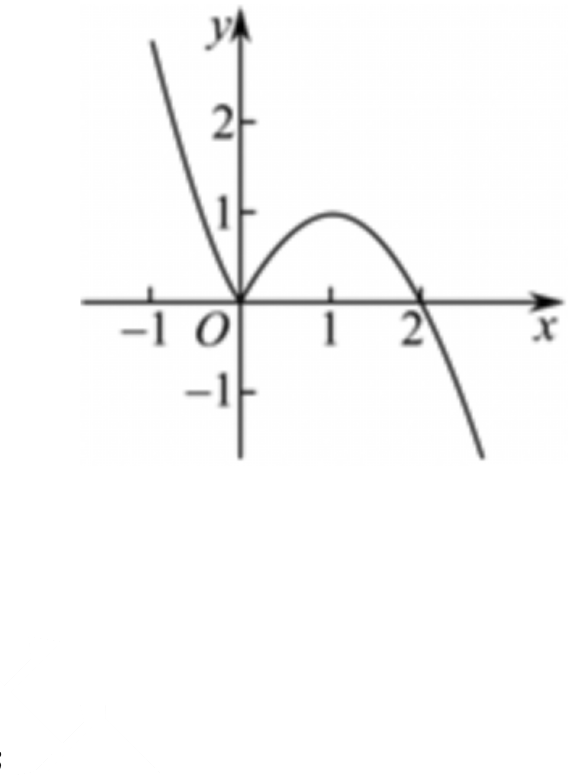
\includegraphics[width=0.20\textwidth]{figures/gao83_q15_graph.png}
\end{center}
\step{由 $[f(x)]^2+af(x)<0$ 得 $[f(x)+a]f(x)<0$，}
\step{当 $a=0$ 时，$[f(x)]^2<0$，不等式无解；}
\step{当 $a>0$ 时，由 $[f(x)+a]f(x)<0$ 得 $-a<f(x)<0$，}
\step{若不等式恰有 $1$ 个整数解，则整数解为 $3$，}
\step{又 $f(3)=-3$，$f(4)=-8$，所以 $-8\leqslant-a<-3$，所以 $3<a\leqslant8$；}
\step{当 $a<0$ 时，由 $[f(x)+a]f(x)<0$ 得 $0<f(x)<-a$，此时有多个解，故舍去；}
\step{综上所述，实数 $a$ 的取值范围为 $(3,8]$. 故选 $C$.}
\solend
\fi

\item 设函数 $f(x)=\begin{cases}\lvert2^x-1\rvert,&x\leqslant2\\ -x+7,&x>2\end{cases}$，若互不相等的实数 $a$、$b$、$c$ 满足 $f(a)=f(b)=f(c)$，
则 $2^a+2^b+2^c$ 的取值范围是\mbox{（\quad）}

\keepwithprev
A. $(8,9)$\qquad B. $(65,129)$\qquad C. $(64,128)$\qquad D. $(66,130)$

\ifanswer
\solbegin
\step{作出函数 $f(x)=\begin{cases}\lvert2^x-1\rvert,&x\leqslant2\\ -x+7,&x>2\end{cases}$ 的图象如图，}
\begin{center}
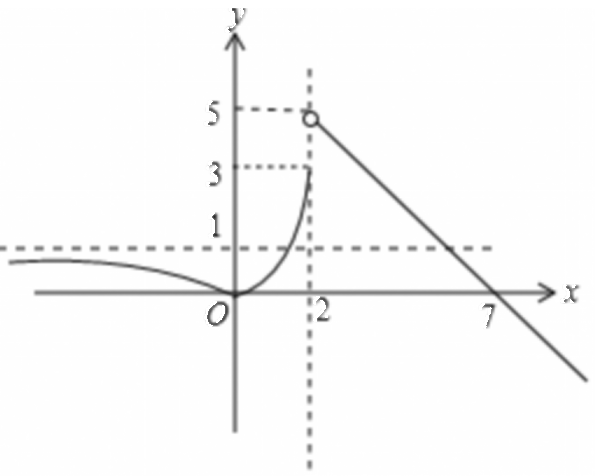
\includegraphics[width=0.22\textwidth]{figures/gao83_q16_graph.png}
\end{center}
\step{不妨设 $a<b<c$，由 $f(a)=f(b)$，得 $1-2^a=2^b-1$，则 $2^a+2^b=2$.}
\step{由 $f(-c)-c+6\in(0,1)$，得 $c\in(6,7)$，则 $64<2^c<128$，}
\step{所以 $66<2^a+2^b+2^c<130$，即 $2^a+2^b+2^c$ 的取值范围是 $(66,130)$. 故选 $D$.}
\solend
\fi

\end{enumerate}

\bigsec{三、解答题}

\begin{enumerate}
\setcounter{enumi}{16}

\item 已知幂函数 $f(x)$ 与一次函数 $g(x)$ 的图象都经过点 $(4,2)$，且 $f(9)=g(5)$.

（1）求 $f(x)$ 与 $g(x)$ 的解析式；

（2）求函数 $h(x)=g(x)-f(x)$ 在 $[0,4]$ 上的值域.

\ansspace*[8]

\ifanswer
\solbegin
\stepm{（1）}{设 $f(x)=x^\alpha$，$g(x)=kx+b$，则 $4^\alpha=2$，即 $\alpha=\dfrac12$，}
\step{$\begin{cases}4k+b=2\\ 3=5k+b\end{cases}$，则 $k=1$，$b=-2$，所以 $f(x)=\sqrt x$，$g(x)=x-2$；}
\stepm{（2）}{$h(x)=g(x)-f(x)=x-\sqrt x-2$，}
\step{令 $t=\sqrt x$，则 $t\in[0,2]$，原函数可化为 $p(t)=t^2-t-2$，}
\step{当 $t=\dfrac12$ 时，函数取得最小值 $-\dfrac94$，当 $t=2$ 时，函数取得最大值 $0$，}
\step{即函数值域为 $\left[-\dfrac94,0\right]$.}
\solend
\fi

\item 目前某县有 $100$ 万人. 经过 $x$ 年后为 $y$ 万人. 如果年平均增长率是 $1.2\%$. 请回答下列问题：

（1）写出 $y$ 关于 $x$ 的函数解析式.

（2）计算 $10$ 年后该县的人口总数（精确到 $0.1$ 万人）.

（3）计算大约多少年后该县的人口总数将达到 $120$ 万（精确到 $1$ 年）.

\ansspace*[9]

\ifanswer
\solbegin
\stepm{（1）}{当 $x=1$ 时，$y=100+100\times1.2\%=100(1+1.2\%)$，}
\step{当 $x=2$ 时，$y=100(1+1.2\%)+100(1+1.2\%)\times1.2\%=100(1+1.2\%)^2$，}
\step{当 $x=3$ 时，$y=100(1+1.2\%)^2+100(1+1.2\%)^2\times1.2\%=100(1+1.2\%)^3$，}
\step{$\cdots\cdots$}
\step{故 $y$ 关于 $x$ 的函数解析式为 $y=100(1+1.2\%)^x\,(x\in\N^*)$；}
\stepm{（2）}{当 $x=10$ 时，$y=100(1+1.2\%)^{10}=100\times1.012^{10}\approx112.7$，}
\step{故 $10$ 年后该县的人口总数约为 $112.7$ 万人；}
\stepm{（3）}{设 $x$ 年后该县的人口总数将达到 $120$ 万，即 $y=100(1+1.2\%)^x=120$，}
\step{解得 $x=\log_{1.012}\dfrac{120}{100}\approx16$，故大约 $16$ 年后该县的人口总数将达到 $120$ 万.}
\solend
\fi

\item 已知 $a>0$ 且 $a\neq1$，$m>0$，函数 $f(x)=(m^2+m-5)a^x$ 是指数函数，且 $f(2)=4$.

（1）求实数 $m$ 和 $a$ 的值；

（2）$f(2x)-2f(x)+2\geqslant nf(x)$ 对任意 $x\in[-1,2]$ 恒成立，求实数 $n$ 的取值范围；

（3）若关于 $x$ 的方程 $f(2x)-(2k+8)f(x)+2k+7b=0$ 有两个不相等的实数根，且一根
大于 $0$，另一根小于 $0$，其中 $k>0$，求整数 $b$ 的最大值.

\ansspace*[11]

\ifanswer
\solbegin
\stepm{（1）}{因为函数 $f(x)=(m^2+m-5)a^x$ 是指数函数，}
\step{所以 $m^2+m-5=1$，即 $m^2+m-6=0$，解得 $m=2$ 或 $m=-3$，}
\step{又 $m>0$，所以 $m=2$，又 $f(2)=a^2=4$，$a>0$ 且 $a\neq1$，所以 $a=2$；}
\stepm{（2）}{由（1）得 $f(x)=2^x$，}
\step{由题意 $2^{2x}-2\cdot2^x+2\geqslant n2^x$ 对任意 $x\in[-1,2]$ 恒成立，}
\step{所以 $n\leqslant2^x-2+\dfrac2{2^x}$ 对任意 $x\in[-1,2]$ 恒成立，则 $n\leqslant\left(2^x-2+\dfrac2{2^x}\right)_{\min}$，}
\step{记 $g(x)=2^x-2+\dfrac2{2^x}$，$x\in[-1,2]$，}
\step{令 $t=2^x$，因为 $x\in[-1,2]$，所以 $t\in\left[\dfrac12,4\right]$，则 $y=t+\dfrac2t-2$，$t\in\left[\dfrac12,4\right]$，}
\step{函数 $y=t+\dfrac2t-2$ 在 $\left[\dfrac12,\sqrt2\right]$ 上严格减，在 $[\sqrt2,4]$ 上严格增，}
\step{所以 $y=t+\dfrac2t-2$ 的最小值为 $\sqrt2+\dfrac2{\sqrt2}-2=2\sqrt2-2$，}
\step{所以 $n\leqslant2\sqrt2-2$，即实数 $n$ 的取值范围为 $(-\infty,2\sqrt2-2]$；}
\stepm{（3）}{方程 $f(2x)-(2k+8)f(x)+2k+7b=0$，}
\step{即方程 $2^{2x}-(2k+8)2^x+2k+7b=0$，即方程 $(2^x)^2-(2k+8)2^x+2k+7b=0$，}
\step{令 $t=2^x>0$，则方程 $t^2-(2k+8)t+2k+7b=0$，}
\step{因为关于 $x$ 的方程 $f(2x)-(2k+8)f(x)+2k+7b=0$ 的一根大于 $0$，另一根小于 $0$，}
\step{所以关于 $t$ 的方程 $t^2-(2k+8)t+2k+7b=0$ 的一根大于 $1$，另一根大于 $0$ 且小于 $1$，}
\step{记 $h(t)=t^2-(2k+8)t+2k+7b$，}
\step{所以 $\begin{cases}h(1)=1^2-(2k+8)\cdot1+2k+7b<0\\ h(0)=2k+7b>0\\ k>0\end{cases}$，所以 $\begin{cases}b<1\\ b>-\dfrac27k\\ k>0\end{cases}$，}
\step{所以整数 $b$ 的最大值为 $0$.}
\solend
\fi

\item 已知幂函数 $f(x)=(p^2-3p+3)x^{p^2-\frac32p-\frac12}$ 满足 $f(2)<f(4)$.

（1）求函数 $f(x)$ 的解析式；

（2）若函数 $g(x)=f^2(x)+mf(x)$，$x\in[1,9]$，是否存在实数 $m$ 使得 $g(x)$ 的最小值为 $0$？
若存在，求出 $m$ 的值；若不存在，说明理由.

（3）若函数 $h(x)=n-f(x+3)$，是否存在实数 $a$、$b\,(a<b)$，使函数 $h(x)$ 在 $[a,b]$ 上的
值域为 $[a,b]$？若存在，求出实数 $n$ 的取值范围；若不存在，说明理由.

\ansspace*[12]

\ifanswer
\solbegin
\stepm{（1）}{因为 $f(x)$ 是幂函数，所以 $p^2-3p+3=1$，解得 $p=1$ 或 $p=2$，}
\step{当 $p=1$ 时，$f(x)=\dfrac1x$，不满足 $f(2)<f(4)$.}
\step{当 $p=2$ 时，$f(x)=\sqrt x$，满足 $f(2)<f(4)$.}
\step{故 $p=2$，函数 $f(x)$ 的解析式为 $f(x)=\sqrt x$；}
\stepm{（2）}{由函数 $g(x)=f^2(x)+mf(x)$，即 $g(x)=(\sqrt x)^2+m\sqrt x$，}
\step{令 $t=\sqrt x$，因为 $x\in[1,9]$，所以 $t\in[1,3]$，}
\step{记 $k(x)=t^2+mt$，其对称轴 $t=-\dfrac m2$，}
\step{①当 $-\dfrac m2\leqslant1$，即 $m\geqslant-2$ 时，则 $k(x)_{\min}=k(1)=1+m=0$，解得 $m=-1$；}
\step{②当 $1<-\dfrac m2<3$ 时，即 $-6<m<-2$，则 $k(x)_{\min}=k\left(-\dfrac m2\right)=-\dfrac{m^2}4=0$，}
\step{解得 $m=0$，不满足，舍去；}
\step{③当 $-\dfrac m2\geqslant3$ 时，即 $m\leqslant-6$ 时，则 $k(x)_{\min}=k(3)=3m+9=0$，解得 $m=-3$，}
\step{不满足，舍去；}
\step{综上所述，存在 $m=-1$ 使得 $g(x)$ 的最小值为 $0$；}
\stepm{（3）}{由函数 $h(x)=n-f(x+3)=n-\sqrt{x+3}$ 在定义域内为严格减函数，}
\step{若存在实数 $a$、$b\,(a<b)$，使函数 $h(x)$ 在 $[a,b]$ 上的值域为 $[a,b]$，}
\step{则 $h(x)=\begin{cases}n-\sqrt{a+3}=b\text{ ①}\\ n-\sqrt{b+3}=a\text{ ②}\end{cases}$，}
\step{两式相减得 $\sqrt{a+3}-\sqrt{b+3}=a-b=(a+3)-(b+3)$，}
\step{所以 $\sqrt{a+3}+\sqrt{b+3}=1$ ③，}
\step{将③代入②得 $n=a+\sqrt{b+3}=a+1-\sqrt{a+3}$，}
\step{令 $t=\sqrt{a+3}$，因为 $a<b$，所以 $0\leqslant t<\dfrac12$，得 $n=t^2-t-2=\left(t-\dfrac12\right)^2-\dfrac94$，}
\step{故实数 $n$ 的取值范围为 $\left(-\dfrac94,-2\right]$.}
\solend
\fi

\item 定理（三角不等式），对于任意的 $a$、$b\in\R$，恒有 $\bigl\lvert\lvert a\rvert-\lvert b\rvert\bigr\rvert\leqslant\lvert a\pm b\rvert\leqslant\lvert a\rvert+\lvert b\rvert$. 定义：
已知 $n\in\N$ 且 $n\geqslant3$，对于有序数组 $a_1$、$a_2$、$\cdots$、$a_n$，称 $\lvert a_1-a_2\rvert+\lvert a_2-a_3\rvert+\cdots+\lvert a_{n-1}-a_n\rvert$
为有序数组 $a_1$、$a_2$、$\cdots$、$a_n$ 的波动距离，记作 $f(a_1,a_2,\cdots,a_n)$，即
$f(a_1,a_2,\cdots,a_n)=\lvert a_1-a_2\rvert+\lvert a_2-a_3\rvert+\cdots+\lvert a_{n-1}-a_n\rvert$，请根据上述信息解决以下几个问题：

（1）求函数 $y=\lvert x-2\rvert+\lvert x-4\rvert$ 的最小值，并指出函数取到最小值时 $x$ 的取值范围；

（2）①求有序数组 $2$、$5$、$3$、$4$ 的波动距离 $f(2,5,3,4)$；

②求证：若 $a$、$b$、$c$、$d\in\R$ 且 $a<b<c$，则 $f(a,b,c,d)\leqslant f(a,c,b,d)$；

（3）同理可证得命题“若 $a$、$b$、$c$、$d\in\R$ 且 $c<b<a$ 时，$f(a,b,c,d)\leqslant f(a,c,b,d)$”也
是真命题（注：该命题无需证明，需要时可直接使用）.

设两两不相等的四个实数 $a_1$、$a_2$、$a_3$、$a_4\in\{3^1,3^2,3^3,3^4\}$，求有序数组 $a_1$、$a_2$、$a_3$、$a_4$ 的
波动距离 $f(a_1,a_2,a_3,a_4)$ 的最大值.

\ansspace*[14]

\ifanswer
\solbegin
\stepm{（1）}{由三角不等式得 $\bigl\lvert\lvert a\rvert-\lvert b\rvert\bigr\rvert\leqslant\lvert a\pm b\rvert\leqslant\lvert a\rvert+\lvert b\rvert$，}
\step{当且仅当 $\lvert a+b\rvert^2=(\lvert a\rvert+\lvert b\rvert)^2$ 时，}
\step{即当 $-ab=\lvert ab\rvert$ 时，即当 $ab\leqslant0$ 时取等号，}
\step{由三角不等式得 $y=\lvert x-2\rvert+\lvert x-4\rvert\geqslant\lvert(x-2)-(x-4)\rvert=2$，}
\step{当且仅当 $(x-2)(x-4)\leqslant0$ 时，即 $2\leqslant x\leqslant4$ 时取等号，}
\step{因此，函数 $y=\lvert x-2\rvert+\lvert x-4\rvert$ 的最小值为 $2$，此时 $x$ 的取值范围是 $[2,4]$.}
\stepm{（2）}{①由题中定义得 $f(2,5,3,4)=\lvert2-5\rvert+\lvert5-3\rvert+\lvert3-4\rvert=6$；}
\step{②$f(a,b,c,d)-f(a,c,b,d)=\lvert a-b\rvert+\lvert c-d\rvert-\lvert a-c\rvert-\lvert b-d\rvert$，}
\step{因为 $a<b<c$，所以 $\lvert a-b\rvert-\lvert a-c\rvert=-\lvert b-c\rvert$，$\lvert c-d\rvert-\lvert b-d\rvert\leqslant\lvert b-c\rvert$，}
\step{所以 $f(a,b,c,d)-f(a,c,b,d)\leqslant0$，即 $f(a,b,c,d)\leqslant f(a,c,b,d)$，}
\stepm{（3）}{$f(a,b,c,d)=\lvert a-b\rvert+\lvert b-c\rvert+\lvert c-d\rvert$}
\step{$=\lvert d-c\rvert+\lvert c-b\rvert+\lvert b-a\rvert=f(d,c,b,a)$，}
\step{当 $f(a_1,a_2,a_3,a_4)$ 取得最大值时，$a_2=\max\{a_1,a_2,a_3\}$ 或 $a_2=\min\{a_1,a_2,a_3\}$，}
\step{同理 $a_3=\max\{a_2,a_3,a_4\}$ 或 $a_3=\min\{a_2,a_3,a_4\}$，}
\step{若 $a_2=\max\{a_1,a_2,a_3\}$，则 $a_2>a_3$，所以 $a_3=\min\{a_2,a_3,a_4\}$，}
\step{故 $f(a_1,a_2,a_3,a_4)=\lvert a_1-a_2\rvert+\lvert a_2-a_3\rvert+\lvert a_3-a_4\rvert=a_2-a_1+a_2-a_3+a_4-a_3$}
\step{$=2a_2+a_4-2a_3-a_1\leqslant2\times3^4+3^3-2\times3^1-3^2=174$，}
\step{当且仅当 $a_1=3^2$，$a_2=3^4$，$a_3=3^1$，$a_4=3^3$ 时取等号，}
\step{所以 $f(3^2,3^4,3^1,3^3)$ 为 $f(a_1,a_2,a_3,a_4)$ 的最大值，}
\step{若 $a_2=\min\{a_1,a_2,a_3\}$，则 $a_2<a_3$，所以 $a_3=\max\{a_2,a_3,a_4\}$，}
\step{同理可得 $f(3^3,3^4,3^1,3^2)$ 为 $f(a_1,a_2,a_3,a_4)$ 的最大值，}
\step{综上所述，$f(a_1,a_2,a_3,a_4)$ 的最大值为 $174$.}
\solend
\fi

\end{enumerate}

\end{document}
"
%
% 原始材料：微信公众号“魔都数学加油站”文章，连载“27学年高一83”；
% 原文标题“27学年高一83——2026-2027年上海市交附闵行高一上周末作业10.23”；
% 原文链接：https://mp.weixin.qq.com/s/t5AfTwQXg4Sj4i_Dl5rgXA。
% 页面标注发布时间 2026-10-26 20:15（上海）。
% 正文为 12 张 PNG 页（`原图/高一83_交附闵行_周末作业10.23/01..12.png`），
% 尺寸混排（第 1—8 页为 4762×6735，第 9—12 页为 2560×3620），均按页序读取。
%
% 篇幅与题号：原卷自第 3 题起编号（第 1、2 题不在原文内）。填空题 3—12（10 题）、
% 选择题 13—16（4 题）、解答题 17—21（5 题），共 19 题。
%
% 讲评版：19 题全部印【解析】，本稿不另提 \ans{}；选择题答案在解析末句“故选 C／B／C／D”。
%
% 副标题：原卷未印副标题。本稿按内容标作“函数与导数”（本卷考幂函数、指数函数、
% 对数与函数应用，属“函数与导数”模块；副标题只用知识模块名，见 README 说明）。
%
% 与原卷的排版差异：
%   ① 原卷每题下直接印【解析】，本稿按全稿惯例将解析置于答案版；
%   ② 原卷未印副标题，本稿补出；填空横线统一排 \blankline[4.4em]；
%   ③ 原卷数集记号排斜体 $R$、$Z$、$N$，本稿按全稿惯例改用 $\R$、$\Z$、$\N$；
%   ④ 第 17—21 题的子问用行内“（1）（2）（3）”段，解析中的子问标号用 \stepm；
%   ⑤ 解答题按惯例加 \ansspace；选择题括号排 \mbox{（\quad）}；
%   ⑥ 第 15、16 题解析各有一幅函数图象，裁自原图（第 6 页）后去粉色水印、转灰度，
%      仅答案版出。
%
% 行数核对：逐题数 \step/\stepm 条数，合计 145 条（Q3：1；Q4：1；Q5：4；Q6：5；
% Q7：2；Q8：7；Q9：10；Q10：5；Q11：6；Q12：8；Q13：3；Q14：4；Q15：8；
% Q16：4；Q17：6；Q18：9；Q19：19；Q20：21；Q21：22）。原卷解析的换行
% 按语意合并，未逐行强拆。
%
\documentclass[a4paper,11pt]{article}
\usepackage{common}

\begin{document}

\examtitlest[4]{2026--2027 年交附闵行高一上周末作业 10.23}{函数与导数}

\bigsec{一、填空题}

\begin{enumerate}
\setcounter{enumi}{2}

\item 已知 $10^a=2$，$10^b=5$，则 $10^{3a-2b}$ 的值为\blankline[4.4em].

\ifanswer
\solbegin
\step{$10^{3a-2b}=\dfrac{10^{3a}}{10^{2b}}=\dfrac{(10^a)^3}{(10^b)^2}=\dfrac{2^3}{5^2}=\dfrac8{25}$.}
\solend
\fi

\item 根式 $a\sqrt{-a}$ 化成分数指数幂是\blankline[4.4em].

\ifanswer
\solbegin
\step{$a\sqrt{-a}=a(-a)^{\frac12}=-(-a)(-a)^{\frac12}=-(-a)^{\frac32}$.}
\solend
\fi

\item 已知数列 $\{a_n\}$ 的通项公式为 $a_n=\left(\dfrac49\right)^{n-1}-\left(\dfrac23\right)^{n-1}$，在下列说法中：①有最大项；
②有最小项；③没有最大项；④没有最小项. 正确的是\blankline[3.6em]（填序号）.

\ifanswer
\solbegin
\step{令 $t=\left(\dfrac23\right)^{n-1}$，则 $t\in\left\{1,\dfrac23,\dfrac49,\dfrac8{27},\cdots\right\}\subset(0,1]$，$t$ 是关于 $n$ 的减函数，}
\step{则 $a_n=t^2-t=\left(t-\dfrac12\right)^2-\dfrac14$，}
\step{所以当 $t=1$ 即 $n=1$ 时 $a_n$ 取得最大为 $0$，当 $t=\dfrac49$ 即 $n=3$ 时 $a_n$ 取得最小为 $-\dfrac{20}{81}$，}
\step{所以 $a_n$ 既有最大项又有最小项，故①和②正确.}
\solend
\fi

\item 已知 $f(x)=\mathrm{e}^{x-\frac12}-\mathrm{e}^{-x+\frac12}+\dfrac{4x}{2x-1}$，则
$f\left(\dfrac1{2020}\right)+f\left(\dfrac2{2020}\right)+f\left(\dfrac3{2020}\right)+\cdots+f\left(\dfrac{1009}{2020}\right)+f\left(\dfrac{1011}{2020}\right)+\cdots+f\left(\dfrac{2019}{2020}\right)$ 的
值为\blankline[4.4em].

\ifanswer
\solbegin
\step{因为 $f(x)+f(1-x)=\mathrm{e}^{x-\frac12}-\mathrm{e}^{-x+\frac12}+\dfrac{4x}{2x-1}+\mathrm{e}^{(1-x)-\frac12}-\mathrm{e}^{-(1-x)+\frac12}+\dfrac{4(1-x)}{2(1-x)-1}$}
\step{$=\dfrac{4x}{2x-1}+\dfrac{4-4x}{1-2x}=\dfrac{4(2x-1)}{2x-1}=4$，}
\step{记 $S=f\left(\dfrac1{2020}\right)+f\left(\dfrac2{2020}\right)+\cdots+f\left(\dfrac{2019}{2020}\right)$，}
\step{又 $S=f\left(\dfrac{2019}{2020}\right)+f\left(\dfrac{2018}{2020}\right)+\cdots+f\left(\dfrac2{2020}\right)+f\left(\dfrac1{2020}\right)$，}
\step{对齐相加得 $2S=2018\times4$，所以 $S=4036$.}
\solend
\fi

\item 不等式 $2^{x^2-2x-3}<\left(\dfrac12\right)^{3(x-1)}$ 的解集为\blankline[4.4em].

\ifanswer
\solbegin
\step{由 $2^{x^2-2x-3}<\left(\dfrac12\right)^{3(x-1)}$ 得 $x^2-2x-3<-3(x-1)$，即 $x^2+x-6<0$，}
\step{故解集为 $(-3,2)$.}
\solend
\fi

\item 函数 $f(x)=x^{\ln5}+x^{\ln12}-13^{\ln x}$ 的零点是\blankline[4.4em]. 附：$a^{\log_bc}=c^{\log_ba}$
（$a>0$，$b>0$，$c>0$，$b\neq1$）.

\ifanswer
\solbegin
\step{函数 $f(x)=x^{\ln5}+x^{\ln12}-13^{\ln x}$，}
\step{若 $f(x)=x^{\ln5}+x^{\ln12}-13^{\ln x}=0$，变形得 $x^{\ln5}+x^{\ln12}=13^{\ln x}$，}
\step{又 $a^{\log_bc}=c^{\log_ba}$（$a>0$，$b>0$，$c>0$，$b\neq1$），得 $5^{\ln x}+12^{\ln x}=13^{\ln x}$，}
\step{令 $g(t)=\left(\dfrac5{13}\right)^t+\left(\dfrac{12}{13}\right)^t-1$，易得 $g(t)$ 严格减，所以 $g(t)=0$ 至多有一解，}
\step{即 $\left(\dfrac5{13}\right)^t+\left(\dfrac{12}{13}\right)^t-1=0$ 至多有一解，变形得方程 $5^t+12^t=13^t$ 至多有一解，}
\step{易得 $t=2$ 时，有 $5^2+12^2=13^2$ 成立，则方程 $5^t+12^t=13^t$ 有唯一解 $t=2$，}
\step{即 $\ln x=2$，解得 $x=\mathrm{e}^2$，即函数 $f(x)$ 的零点为 $\mathrm{e}^2$.}
\solend
\fi

\item 已知幂函数 $f(x)=(m^2-2m-2)x^{m^2+m-2}$ 在 $(0,+\infty)$ 上是严格减函数，则不等式
$f(x-1)<f(3-2x)$ 的解集为\blankline[4.4em].

\ifanswer
\solbegin
\step{因为 $f(x)$ 为幂函数，所以 $m^2-2m-2=1$，解得 $m=-1$ 或 $m=3$；}
\step{当 $m=3$ 时，$f(x)=x^{10}$ 在 $(0,+\infty)$ 上严格增，不合题意；}
\step{当 $m=-1$ 时，$f(x)=x^{-2}$ 在 $(0,+\infty)$ 上严格减，符合题意；}
\step{综上所述，$m=-1$；}
\step{因为 $f(x)=x^{-2}$ 的定义域为 $(-\infty,0)\cup(0,+\infty)$，$f(-x)=(-x)^{-2}=x^{-2}=f(x)$，}
\step{所以 $f(x)$ 为定义在 $(-\infty,0)\cup(0,+\infty)$ 上的偶函数，}
\step{故 $f(x-1)=f(\lvert x-1\rvert)$，$f(3-2x)=f(\lvert3-2x\rvert)$，}
\step{$f(x-1)<f(3-2x)\Rightarrow f(\lvert x-1\rvert)<f(\lvert3-2x\rvert)\Rightarrow\lvert x-1\rvert>\lvert3-2x\rvert$}
\step{且 $\lvert x-1\rvert\neq0$，$\lvert3-2x\rvert\neq0$，解得 $\dfrac43<x<\dfrac32$ 或 $\dfrac32<x<2$，}
\step{所以 $f(x-1)<f(3-2x)$ 的解集为 $\left(\dfrac43,\dfrac32\right)\cup\left(\dfrac32,2\right)$.}
\solend
\fi

\item 若实数 $x_1$、$x_2$ 满足 $\mathrm{e}^{x_1}+x_1-3=0$，$x_2\ln x_2+3x_2-1=0$，则 $\dfrac{x_1x_2+1}{x_2}$ 的值为\blankline[4.4em].

\ifanswer
\solbegin
\step{易得 $x_2>0$，则 $\ln x_2+3-\dfrac1{x_2}=0$，即 $\mathrm{e}^{-\ln x_2}+(-\ln x_2)-3=0$.}
\step{设 $f(x)=\mathrm{e}^x+x-3$，则函数 $f(x)$ 在 $(-\infty,+\infty)$ 上严格增.}
\step{由 $\mathrm{e}^{x_1}+x_1-3=0$，$\mathrm{e}^{-\ln x_2}+(-\ln x_2)-3=0$，得 $f(x_1)=0$，$f(-\ln x_2)=0$，}
\step{所以 $f(x_1)=f(-\ln x_2)$，得 $x_1=-\ln x_2$，即 $\ln x_2=-x_1$，所以 $x_2=\mathrm{e}^{-x_1}$，得 $\dfrac1{x_2}=\mathrm{e}^{x_1}$.}
\step{因为 $\mathrm{e}^{x_1}+x_1-3=0$，所以 $\mathrm{e}^{x_1}+x_1=3$，所以 $\dfrac{x_1x_2+1}{x_2}=x_1+\dfrac1{x_2}=\mathrm{e}^{x_1}+x_1=3$.}
\solend
\fi

\item 已知 $\alpha$、$\beta$ 是方程 $9^x-2m\cdot3^x+m^2-1=0$ 的两个根，若 $\alpha+\beta=1$，则 $\alpha\beta=\blankline[4.4em]$.

\ifanswer
\solbegin
\step{由题意得方程 $9^x-2m\cdot3^x+m^2-1=0$ 有两个根，}
\step{则方程 $t^2-2mt+m^2-1=0$ 有二正根，则 $\begin{cases}\Delta=4m^2-4(m^2-1)\geqslant0\\ 2m>0\\ m^2-1>0\end{cases}$，解得 $m>1$，}
\step{又 $\alpha$、$\beta$ 是方程 $9^x-2m\cdot3^x+m^2-1=0$ 的两个根，则 $3^\alpha\times3^\beta=m^2-1$，}
\step{又 $\alpha+\beta=1$，则 $m^2-1=3^{\alpha+\beta}=3$，解得 $m=2$ 或 $m=-2$（舍），}
\step{则 $3^\alpha+3^\beta=2m=4$，又 $\alpha=1-\beta$，则 $3^{1-\beta}+3^\beta=4$，解得 $\beta=0$ 或 $\beta=1$，}
\step{则 $\begin{cases}\alpha=1\\ \beta=0\end{cases}$ 或 $\begin{cases}\alpha=0\\ \beta=1\end{cases}$，则 $\alpha\beta=0$.}
\solend
\fi

\item 已知实数 $a,b,c\in(1,+\infty)$，满足 $a^{\log_ba}\cdot b^{\log_cb}\cdot c^{\log_ac}=100$，则 $abc$ 的最大值为\blankline[4.4em].

\ifanswer
\solbegin
\step{由换底公式得 $\log_ba=\dfrac{\ln a}{\ln b}$，$\log_cb=\dfrac{\ln b}{\ln c}$，$\log_ac=\dfrac{\ln c}{\ln a}$，}
\step{设 $X=\ln a$，$Y=\ln b$，$Z=\ln c$，得 $a=\mathrm{e}^X$，$b=\mathrm{e}^Y$，$c=\mathrm{e}^Z$，}
\step{代入得 $a^{\log_ba}\cdot b^{\log_cb}\cdot c^{\log_ac}=a^{\frac{\ln a}{\ln b}}\cdot b^{\frac{\ln b}{\ln c}}\cdot c^{\frac{\ln c}{\ln a}}=(\mathrm{e}^X)^{\frac XY}\cdot(\mathrm{e}^Y)^{\frac YZ}\cdot(\mathrm{e}^Z)^{\frac ZX}=100$，}
\step{即 $\mathrm{e}^{\frac{X^2}Y+\frac{Y^2}Z+\frac{Z^2}X}=100$，两边取对数得 $\dfrac{X^2}Y+\dfrac{Y^2}Z+\dfrac{Z^2}X=\ln100$.}
\step{由 $a,b,c\in(1,+\infty)$，得 $X>0$，$Y>0$，$Z>0$，}
\step{由柯西不等式，得 $\left(\dfrac{X^2}Y+\dfrac{Y^2}Z+\dfrac{Z^2}X\right)(X+Y+Z)\geqslant(X+Y+Z)^2$，}
\step{即 $X+Y+Z\leqslant\dfrac{X^2}Y+\dfrac{Y^2}Z+\dfrac{Z^2}X=\ln100$，当且仅当 $X=Y=Z$ 时取等号，}
\step{因此 $(X+Y+Z)_{\max}=\ln100$，所以 $(abc)_{\max}=\mathrm{e}^{(X+Y+Z)_{\max}}=\mathrm{e}^{\ln100}=100$.}
\solend
\fi

\end{enumerate}

\bigsec{二、选择题}

\begin{enumerate}
\setcounter{enumi}{12}

\item 已知集合 $A=\{x\mid x=2k,k\in\Z\}$，$B=\{x\mid x=4k+2,\,k\in\Z\}$，则 $A\cup B=\mbox{（\quad）}$

\keepwithprev
A. $B$\qquad B. $\R$\qquad C. $A$\qquad D. 以上都不是

\ifanswer
\solbegin
\step{$B=\{x\mid x=4k+2,k\in\Z\}=\{x\mid x=2(2k+1),k\in\Z\}$，它表示奇数的 $2$ 倍组成的集合，}
\step{$A=\{x\mid x=2k,k\in\Z\}$，即集合 $A$ 是整数的 $2$ 倍组成的集合，}
\step{则 $B\subseteq A$，则 $A\cup B=A$. 故选 $C$.}
\solend
\fi

\item 教室通风的目的是通过空气的流动，排出室内的污浊空气和致病微生物，降低室内二氧化碳和致病微生物的浓度，送进室外的新鲜空气. 按照国家标准，教室内空气中二氧化碳日平均最高容许浓度应小于等于 $0.1\%$. 经测定，刚下课时，空气中含有 $0.2\%$ 的二氧化碳，若开窗通风后教室内二氧化碳的浓度为 $y\%$，且 $y$ 随时间 $t$（单位：分钟）的变化规律可以用函数 $y=0.05+\lambda\mathrm{e}^{-\frac t{12}}\,(\lambda\in\R)$ 描述，则该教室内的二氧化碳浓度达到国家标准至少需要的时间为\mbox{（\quad）}

\keepwithprev
A. $10$ 分钟\qquad B. $14$ 分钟\qquad C. $15$ 分钟\qquad D. $20$ 分钟

\ifanswer
\solbegin
\step{由题意得，当 $t=0$ 时，$y=0.2$，即 $0.05+\lambda\mathrm{e}^0=0.2$，解得 $\lambda=0.15$，}
\step{所以 $y=0.05+0.15\mathrm{e}^{-\frac t{12}}$，由题意得 $0.05+0.15\mathrm{e}^{-\frac t{12}}\leqslant0.1$，即 $\mathrm{e}^{-\frac t{12}}\leqslant\dfrac13$，}
\step{两边取对数得 $-\dfrac t{12}\leqslant-\ln3$，所以 $t\geqslant12\ln3\approx13.2$，}
\step{所以该教室内的二氧化碳浓度达到国家标准至少需要的时间为 $14$ 分钟. 故选 $B$.}
\solend
\fi

\item 已知函数 $f(x)=\begin{cases}-x^2+2x,&x\geqslant0\\ x^2-2x,&x<0\end{cases}$，若关于 $x$ 的不等式 $[f(x)]^2+af(x)<0$ 恰有 $1$ 个整数
解，则实数 $a$ 的最大值为\mbox{（\quad）}

\keepwithprev
A. $-2$\qquad B. $3$\qquad C. $8$\qquad D. $9$

\ifanswer
\solbegin
\step{作出 $f(x)$ 的图象，如图所示：}
\begin{center}
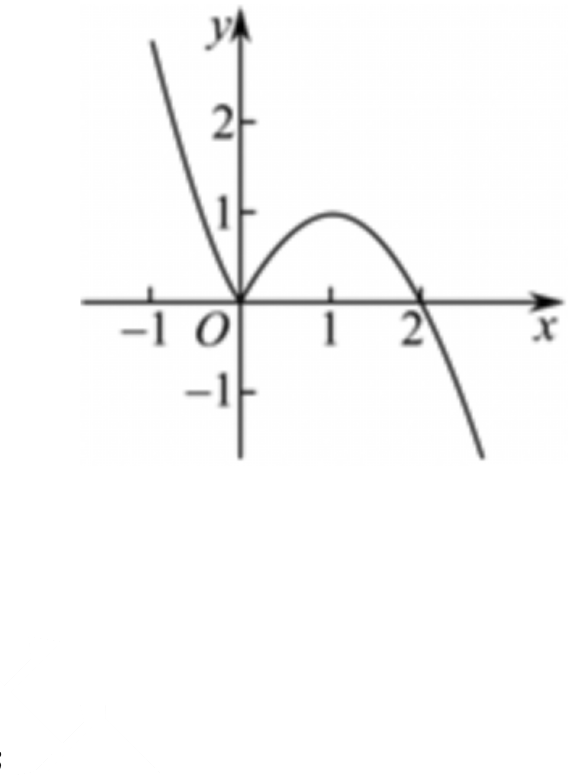
\includegraphics[width=0.20\textwidth]{figures/gao83_q15_graph.png}
\end{center}
\step{由 $[f(x)]^2+af(x)<0$ 得 $[f(x)+a]f(x)<0$，}
\step{当 $a=0$ 时，$[f(x)]^2<0$，不等式无解；}
\step{当 $a>0$ 时，由 $[f(x)+a]f(x)<0$ 得 $-a<f(x)<0$，}
\step{若不等式恰有 $1$ 个整数解，则整数解为 $3$，}
\step{又 $f(3)=-3$，$f(4)=-8$，所以 $-8\leqslant-a<-3$，所以 $3<a\leqslant8$；}
\step{当 $a<0$ 时，由 $[f(x)+a]f(x)<0$ 得 $0<f(x)<-a$，此时有多个解，故舍去；}
\step{综上所述，实数 $a$ 的取值范围为 $(3,8]$. 故选 $C$.}
\solend
\fi

\item 设函数 $f(x)=\begin{cases}\lvert2^x-1\rvert,&x\leqslant2\\ -x+7,&x>2\end{cases}$，若互不相等的实数 $a$、$b$、$c$ 满足 $f(a)=f(b)=f(c)$，
则 $2^a+2^b+2^c$ 的取值范围是\mbox{（\quad）}

\keepwithprev
A. $(8,9)$\qquad B. $(65,129)$\qquad C. $(64,128)$\qquad D. $(66,130)$

\ifanswer
\solbegin
\step{作出函数 $f(x)=\begin{cases}\lvert2^x-1\rvert,&x\leqslant2\\ -x+7,&x>2\end{cases}$ 的图象如图，}
\begin{center}
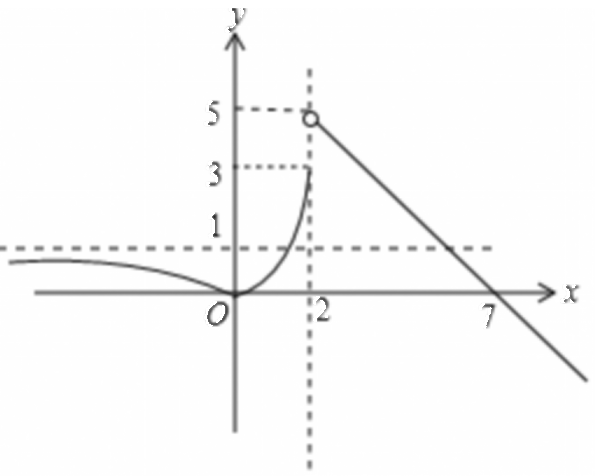
\includegraphics[width=0.22\textwidth]{figures/gao83_q16_graph.png}
\end{center}
\step{不妨设 $a<b<c$，由 $f(a)=f(b)$，得 $1-2^a=2^b-1$，则 $2^a+2^b=2$.}
\step{由 $f(-c)-c+6\in(0,1)$，得 $c\in(6,7)$，则 $64<2^c<128$，}
\step{所以 $66<2^a+2^b+2^c<130$，即 $2^a+2^b+2^c$ 的取值范围是 $(66,130)$. 故选 $D$.}
\solend
\fi

\end{enumerate}

\bigsec{三、解答题}

\begin{enumerate}
\setcounter{enumi}{16}

\item 已知幂函数 $f(x)$ 与一次函数 $g(x)$ 的图象都经过点 $(4,2)$，且 $f(9)=g(5)$.

（1）求 $f(x)$ 与 $g(x)$ 的解析式；

（2）求函数 $h(x)=g(x)-f(x)$ 在 $[0,4]$ 上的值域.

\ansspace*[8]

\ifanswer
\solbegin
\stepm{（1）}{设 $f(x)=x^\alpha$，$g(x)=kx+b$，则 $4^\alpha=2$，即 $\alpha=\dfrac12$，}
\step{$\begin{cases}4k+b=2\\ 3=5k+b\end{cases}$，则 $k=1$，$b=-2$，所以 $f(x)=\sqrt x$，$g(x)=x-2$；}
\stepm{（2）}{$h(x)=g(x)-f(x)=x-\sqrt x-2$，}
\step{令 $t=\sqrt x$，则 $t\in[0,2]$，原函数可化为 $p(t)=t^2-t-2$，}
\step{当 $t=\dfrac12$ 时，函数取得最小值 $-\dfrac94$，当 $t=2$ 时，函数取得最大值 $0$，}
\step{即函数值域为 $\left[-\dfrac94,0\right]$.}
\solend
\fi

\item 目前某县有 $100$ 万人. 经过 $x$ 年后为 $y$ 万人. 如果年平均增长率是 $1.2\%$. 请回答下列问题：

（1）写出 $y$ 关于 $x$ 的函数解析式.

（2）计算 $10$ 年后该县的人口总数（精确到 $0.1$ 万人）.

（3）计算大约多少年后该县的人口总数将达到 $120$ 万（精确到 $1$ 年）.

\ansspace*[9]

\ifanswer
\solbegin
\stepm{（1）}{当 $x=1$ 时，$y=100+100\times1.2\%=100(1+1.2\%)$，}
\step{当 $x=2$ 时，$y=100(1+1.2\%)+100(1+1.2\%)\times1.2\%=100(1+1.2\%)^2$，}
\step{当 $x=3$ 时，$y=100(1+1.2\%)^2+100(1+1.2\%)^2\times1.2\%=100(1+1.2\%)^3$，}
\step{$\cdots\cdots$}
\step{故 $y$ 关于 $x$ 的函数解析式为 $y=100(1+1.2\%)^x\,(x\in\N^*)$；}
\stepm{（2）}{当 $x=10$ 时，$y=100(1+1.2\%)^{10}=100\times1.012^{10}\approx112.7$，}
\step{故 $10$ 年后该县的人口总数约为 $112.7$ 万人；}
\stepm{（3）}{设 $x$ 年后该县的人口总数将达到 $120$ 万，即 $y=100(1+1.2\%)^x=120$，}
\step{解得 $x=\log_{1.012}\dfrac{120}{100}\approx16$，故大约 $16$ 年后该县的人口总数将达到 $120$ 万.}
\solend
\fi

\item 已知 $a>0$ 且 $a\neq1$，$m>0$，函数 $f(x)=(m^2+m-5)a^x$ 是指数函数，且 $f(2)=4$.

（1）求实数 $m$ 和 $a$ 的值；

（2）$f(2x)-2f(x)+2\geqslant nf(x)$ 对任意 $x\in[-1,2]$ 恒成立，求实数 $n$ 的取值范围；

（3）若关于 $x$ 的方程 $f(2x)-(2k+8)f(x)+2k+7b=0$ 有两个不相等的实数根，且一根
大于 $0$，另一根小于 $0$，其中 $k>0$，求整数 $b$ 的最大值.

\ansspace*[11]

\ifanswer
\solbegin
\stepm{（1）}{因为函数 $f(x)=(m^2+m-5)a^x$ 是指数函数，}
\step{所以 $m^2+m-5=1$，即 $m^2+m-6=0$，解得 $m=2$ 或 $m=-3$，}
\step{又 $m>0$，所以 $m=2$，又 $f(2)=a^2=4$，$a>0$ 且 $a\neq1$，所以 $a=2$；}
\stepm{（2）}{由（1）得 $f(x)=2^x$，}
\step{由题意 $2^{2x}-2\cdot2^x+2\geqslant n2^x$ 对任意 $x\in[-1,2]$ 恒成立，}
\step{所以 $n\leqslant2^x-2+\dfrac2{2^x}$ 对任意 $x\in[-1,2]$ 恒成立，则 $n\leqslant\left(2^x-2+\dfrac2{2^x}\right)_{\min}$，}
\step{记 $g(x)=2^x-2+\dfrac2{2^x}$，$x\in[-1,2]$，}
\step{令 $t=2^x$，因为 $x\in[-1,2]$，所以 $t\in\left[\dfrac12,4\right]$，则 $y=t+\dfrac2t-2$，$t\in\left[\dfrac12,4\right]$，}
\step{函数 $y=t+\dfrac2t-2$ 在 $\left[\dfrac12,\sqrt2\right]$ 上严格减，在 $[\sqrt2,4]$ 上严格增，}
\step{所以 $y=t+\dfrac2t-2$ 的最小值为 $\sqrt2+\dfrac2{\sqrt2}-2=2\sqrt2-2$，}
\step{所以 $n\leqslant2\sqrt2-2$，即实数 $n$ 的取值范围为 $(-\infty,2\sqrt2-2]$；}
\stepm{（3）}{方程 $f(2x)-(2k+8)f(x)+2k+7b=0$，}
\step{即方程 $2^{2x}-(2k+8)2^x+2k+7b=0$，即方程 $(2^x)^2-(2k+8)2^x+2k+7b=0$，}
\step{令 $t=2^x>0$，则方程 $t^2-(2k+8)t+2k+7b=0$，}
\step{因为关于 $x$ 的方程 $f(2x)-(2k+8)f(x)+2k+7b=0$ 的一根大于 $0$，另一根小于 $0$，}
\step{所以关于 $t$ 的方程 $t^2-(2k+8)t+2k+7b=0$ 的一根大于 $1$，另一根大于 $0$ 且小于 $1$，}
\step{记 $h(t)=t^2-(2k+8)t+2k+7b$，}
\step{所以 $\begin{cases}h(1)=1^2-(2k+8)\cdot1+2k+7b<0\\ h(0)=2k+7b>0\\ k>0\end{cases}$，所以 $\begin{cases}b<1\\ b>-\dfrac27k\\ k>0\end{cases}$，}
\step{所以整数 $b$ 的最大值为 $0$.}
\solend
\fi

\item 已知幂函数 $f(x)=(p^2-3p+3)x^{p^2-\frac32p-\frac12}$ 满足 $f(2)<f(4)$.

（1）求函数 $f(x)$ 的解析式；

（2）若函数 $g(x)=f^2(x)+mf(x)$，$x\in[1,9]$，是否存在实数 $m$ 使得 $g(x)$ 的最小值为 $0$？
若存在，求出 $m$ 的值；若不存在，说明理由.

（3）若函数 $h(x)=n-f(x+3)$，是否存在实数 $a$、$b\,(a<b)$，使函数 $h(x)$ 在 $[a,b]$ 上的
值域为 $[a,b]$？若存在，求出实数 $n$ 的取值范围；若不存在，说明理由.

\ansspace*[12]

\ifanswer
\solbegin
\stepm{（1）}{因为 $f(x)$ 是幂函数，所以 $p^2-3p+3=1$，解得 $p=1$ 或 $p=2$，}
\step{当 $p=1$ 时，$f(x)=\dfrac1x$，不满足 $f(2)<f(4)$.}
\step{当 $p=2$ 时，$f(x)=\sqrt x$，满足 $f(2)<f(4)$.}
\step{故 $p=2$，函数 $f(x)$ 的解析式为 $f(x)=\sqrt x$；}
\stepm{（2）}{由函数 $g(x)=f^2(x)+mf(x)$，即 $g(x)=(\sqrt x)^2+m\sqrt x$，}
\step{令 $t=\sqrt x$，因为 $x\in[1,9]$，所以 $t\in[1,3]$，}
\step{记 $k(x)=t^2+mt$，其对称轴 $t=-\dfrac m2$，}
\step{①当 $-\dfrac m2\leqslant1$，即 $m\geqslant-2$ 时，则 $k(x)_{\min}=k(1)=1+m=0$，解得 $m=-1$；}
\step{②当 $1<-\dfrac m2<3$ 时，即 $-6<m<-2$，则 $k(x)_{\min}=k\left(-\dfrac m2\right)=-\dfrac{m^2}4=0$，}
\step{解得 $m=0$，不满足，舍去；}
\step{③当 $-\dfrac m2\geqslant3$ 时，即 $m\leqslant-6$ 时，则 $k(x)_{\min}=k(3)=3m+9=0$，解得 $m=-3$，}
\step{不满足，舍去；}
\step{综上所述，存在 $m=-1$ 使得 $g(x)$ 的最小值为 $0$；}
\stepm{（3）}{由函数 $h(x)=n-f(x+3)=n-\sqrt{x+3}$ 在定义域内为严格减函数，}
\step{若存在实数 $a$、$b\,(a<b)$，使函数 $h(x)$ 在 $[a,b]$ 上的值域为 $[a,b]$，}
\step{则 $h(x)=\begin{cases}n-\sqrt{a+3}=b\text{ ①}\\ n-\sqrt{b+3}=a\text{ ②}\end{cases}$，}
\step{两式相减得 $\sqrt{a+3}-\sqrt{b+3}=a-b=(a+3)-(b+3)$，}
\step{所以 $\sqrt{a+3}+\sqrt{b+3}=1$ ③，}
\step{将③代入②得 $n=a+\sqrt{b+3}=a+1-\sqrt{a+3}$，}
\step{令 $t=\sqrt{a+3}$，因为 $a<b$，所以 $0\leqslant t<\dfrac12$，得 $n=t^2-t-2=\left(t-\dfrac12\right)^2-\dfrac94$，}
\step{故实数 $n$ 的取值范围为 $\left(-\dfrac94,-2\right]$.}
\solend
\fi

\item 定理（三角不等式），对于任意的 $a$、$b\in\R$，恒有 $\bigl\lvert\lvert a\rvert-\lvert b\rvert\bigr\rvert\leqslant\lvert a\pm b\rvert\leqslant\lvert a\rvert+\lvert b\rvert$. 定义：
已知 $n\in\N$ 且 $n\geqslant3$，对于有序数组 $a_1$、$a_2$、$\cdots$、$a_n$，称 $\lvert a_1-a_2\rvert+\lvert a_2-a_3\rvert+\cdots+\lvert a_{n-1}-a_n\rvert$
为有序数组 $a_1$、$a_2$、$\cdots$、$a_n$ 的波动距离，记作 $f(a_1,a_2,\cdots,a_n)$，即
$f(a_1,a_2,\cdots,a_n)=\lvert a_1-a_2\rvert+\lvert a_2-a_3\rvert+\cdots+\lvert a_{n-1}-a_n\rvert$，请根据上述信息解决以下几个问题：

（1）求函数 $y=\lvert x-2\rvert+\lvert x-4\rvert$ 的最小值，并指出函数取到最小值时 $x$ 的取值范围；

（2）①求有序数组 $2$、$5$、$3$、$4$ 的波动距离 $f(2,5,3,4)$；

②求证：若 $a$、$b$、$c$、$d\in\R$ 且 $a<b<c$，则 $f(a,b,c,d)\leqslant f(a,c,b,d)$；

（3）同理可证得命题“若 $a$、$b$、$c$、$d\in\R$ 且 $c<b<a$ 时，$f(a,b,c,d)\leqslant f(a,c,b,d)$”也
是真命题（注：该命题无需证明，需要时可直接使用）.

设两两不相等的四个实数 $a_1$、$a_2$、$a_3$、$a_4\in\{3^1,3^2,3^3,3^4\}$，求有序数组 $a_1$、$a_2$、$a_3$、$a_4$ 的
波动距离 $f(a_1,a_2,a_3,a_4)$ 的最大值.

\ansspace*[14]

\ifanswer
\solbegin
\stepm{（1）}{由三角不等式得 $\bigl\lvert\lvert a\rvert-\lvert b\rvert\bigr\rvert\leqslant\lvert a\pm b\rvert\leqslant\lvert a\rvert+\lvert b\rvert$，}
\step{当且仅当 $\lvert a+b\rvert^2=(\lvert a\rvert+\lvert b\rvert)^2$ 时，}
\step{即当 $-ab=\lvert ab\rvert$ 时，即当 $ab\leqslant0$ 时取等号，}
\step{由三角不等式得 $y=\lvert x-2\rvert+\lvert x-4\rvert\geqslant\lvert(x-2)-(x-4)\rvert=2$，}
\step{当且仅当 $(x-2)(x-4)\leqslant0$ 时，即 $2\leqslant x\leqslant4$ 时取等号，}
\step{因此，函数 $y=\lvert x-2\rvert+\lvert x-4\rvert$ 的最小值为 $2$，此时 $x$ 的取值范围是 $[2,4]$.}
\stepm{（2）}{①由题中定义得 $f(2,5,3,4)=\lvert2-5\rvert+\lvert5-3\rvert+\lvert3-4\rvert=6$；}
\step{②$f(a,b,c,d)-f(a,c,b,d)=\lvert a-b\rvert+\lvert c-d\rvert-\lvert a-c\rvert-\lvert b-d\rvert$，}
\step{因为 $a<b<c$，所以 $\lvert a-b\rvert-\lvert a-c\rvert=-\lvert b-c\rvert$，$\lvert c-d\rvert-\lvert b-d\rvert\leqslant\lvert b-c\rvert$，}
\step{所以 $f(a,b,c,d)-f(a,c,b,d)\leqslant0$，即 $f(a,b,c,d)\leqslant f(a,c,b,d)$，}
\stepm{（3）}{$f(a,b,c,d)=\lvert a-b\rvert+\lvert b-c\rvert+\lvert c-d\rvert$}
\step{$=\lvert d-c\rvert+\lvert c-b\rvert+\lvert b-a\rvert=f(d,c,b,a)$，}
\step{当 $f(a_1,a_2,a_3,a_4)$ 取得最大值时，$a_2=\max\{a_1,a_2,a_3\}$ 或 $a_2=\min\{a_1,a_2,a_3\}$，}
\step{同理 $a_3=\max\{a_2,a_3,a_4\}$ 或 $a_3=\min\{a_2,a_3,a_4\}$，}
\step{若 $a_2=\max\{a_1,a_2,a_3\}$，则 $a_2>a_3$，所以 $a_3=\min\{a_2,a_3,a_4\}$，}
\step{故 $f(a_1,a_2,a_3,a_4)=\lvert a_1-a_2\rvert+\lvert a_2-a_3\rvert+\lvert a_3-a_4\rvert=a_2-a_1+a_2-a_3+a_4-a_3$}
\step{$=2a_2+a_4-2a_3-a_1\leqslant2\times3^4+3^3-2\times3^1-3^2=174$，}
\step{当且仅当 $a_1=3^2$，$a_2=3^4$，$a_3=3^1$，$a_4=3^3$ 时取等号，}
\step{所以 $f(3^2,3^4,3^1,3^3)$ 为 $f(a_1,a_2,a_3,a_4)$ 的最大值，}
\step{若 $a_2=\min\{a_1,a_2,a_3\}$，则 $a_2<a_3$，所以 $a_3=\max\{a_2,a_3,a_4\}$，}
\step{同理可得 $f(3^3,3^4,3^1,3^2)$ 为 $f(a_1,a_2,a_3,a_4)$ 的最大值，}
\step{综上所述，$f(a_1,a_2,a_3,a_4)$ 的最大值为 $174$.}
\solend
\fi

\end{enumerate}

\end{document}
"
%
% 原始材料：微信公众号“魔都数学加油站”文章，连载“27学年高一83”；
% 原文标题“27学年高一83——2026-2027年上海市交附闵行高一上周末作业10.23”；
% 原文链接：https://mp.weixin.qq.com/s/t5AfTwQXg4Sj4i_Dl5rgXA。
% 页面标注发布时间 2026-10-26 20:15（上海）。
% 正文为 12 张 PNG 页（`原图/高一83_交附闵行_周末作业10.23/01..12.png`），
% 尺寸混排（第 1—8 页为 4762×6735，第 9—12 页为 2560×3620），均按页序读取。
%
% 篇幅与题号：原卷自第 3 题起编号（第 1、2 题不在原文内）。填空题 3—12（10 题）、
% 选择题 13—16（4 题）、解答题 17—21（5 题），共 19 题。
%
% 讲评版：19 题全部印【解析】，本稿不另提 \ans{}；选择题答案在解析末句“故选 C／B／C／D”。
%
% 副标题：原卷未印副标题。本稿按内容标作“函数与导数”（本卷考幂函数、指数函数、
% 对数与函数应用，属“函数与导数”模块；副标题只用知识模块名，见 README 说明）。
%
% 与原卷的排版差异：
%   ① 原卷每题下直接印【解析】，本稿按全稿惯例将解析置于答案版；
%   ② 原卷未印副标题，本稿补出；填空横线统一排 \blankline[4.4em]；
%   ③ 原卷数集记号排斜体 $R$、$Z$、$N$，本稿按全稿惯例改用 $\R$、$\Z$、$\N$；
%   ④ 第 17—21 题的子问用行内“（1）（2）（3）”段，解析中的子问标号用 \stepm；
%   ⑤ 解答题按惯例加 \ansspace；选择题括号排 \mbox{（\quad）}；
%   ⑥ 第 15、16 题解析各有一幅函数图象，裁自原图（第 6 页）后去粉色水印、转灰度，
%      仅答案版出。
%
% 行数核对：逐题数 \step/\stepm 条数，合计 145 条（Q3：1；Q4：1；Q5：4；Q6：5；
% Q7：2；Q8：7；Q9：10；Q10：5；Q11：6；Q12：8；Q13：3；Q14：4；Q15：8；
% Q16：4；Q17：6；Q18：9；Q19：19；Q20：21；Q21：22）。原卷解析的换行
% 按语意合并，未逐行强拆。
%
\documentclass[a4paper,11pt]{article}
\usepackage{common}

\begin{document}

\examtitlest[4]{2026--2027 年交附闵行高一上周末作业 10.23}{函数与导数}

\bigsec{一、填空题}

\begin{enumerate}
\setcounter{enumi}{2}

\item 已知 $10^a=2$，$10^b=5$，则 $10^{3a-2b}$ 的值为\blankline[4.4em].

\ifanswer
\solbegin
\step{$10^{3a-2b}=\dfrac{10^{3a}}{10^{2b}}=\dfrac{(10^a)^3}{(10^b)^2}=\dfrac{2^3}{5^2}=\dfrac8{25}$.}
\solend
\fi

\item 根式 $a\sqrt{-a}$ 化成分数指数幂是\blankline[4.4em].

\ifanswer
\solbegin
\step{$a\sqrt{-a}=a(-a)^{\frac12}=-(-a)(-a)^{\frac12}=-(-a)^{\frac32}$.}
\solend
\fi

\item 已知数列 $\{a_n\}$ 的通项公式为 $a_n=\left(\dfrac49\right)^{n-1}-\left(\dfrac23\right)^{n-1}$，在下列说法中：①有最大项；
②有最小项；③没有最大项；④没有最小项. 正确的是\blankline[3.6em]（填序号）.

\ifanswer
\solbegin
\step{令 $t=\left(\dfrac23\right)^{n-1}$，则 $t\in\left\{1,\dfrac23,\dfrac49,\dfrac8{27},\cdots\right\}\subset(0,1]$，$t$ 是关于 $n$ 的减函数，}
\step{则 $a_n=t^2-t=\left(t-\dfrac12\right)^2-\dfrac14$，}
\step{所以当 $t=1$ 即 $n=1$ 时 $a_n$ 取得最大为 $0$，当 $t=\dfrac49$ 即 $n=3$ 时 $a_n$ 取得最小为 $-\dfrac{20}{81}$，}
\step{所以 $a_n$ 既有最大项又有最小项，故①和②正确.}
\solend
\fi

\item 已知 $f(x)=\mathrm{e}^{x-\frac12}-\mathrm{e}^{-x+\frac12}+\dfrac{4x}{2x-1}$，则
$f\left(\dfrac1{2020}\right)+f\left(\dfrac2{2020}\right)+f\left(\dfrac3{2020}\right)+\cdots+f\left(\dfrac{1009}{2020}\right)+f\left(\dfrac{1011}{2020}\right)+\cdots+f\left(\dfrac{2019}{2020}\right)$ 的
值为\blankline[4.4em].

\ifanswer
\solbegin
\step{因为 $f(x)+f(1-x)=\mathrm{e}^{x-\frac12}-\mathrm{e}^{-x+\frac12}+\dfrac{4x}{2x-1}+\mathrm{e}^{(1-x)-\frac12}-\mathrm{e}^{-(1-x)+\frac12}+\dfrac{4(1-x)}{2(1-x)-1}$}
\step{$=\dfrac{4x}{2x-1}+\dfrac{4-4x}{1-2x}=\dfrac{4(2x-1)}{2x-1}=4$，}
\step{记 $S=f\left(\dfrac1{2020}\right)+f\left(\dfrac2{2020}\right)+\cdots+f\left(\dfrac{2019}{2020}\right)$，}
\step{又 $S=f\left(\dfrac{2019}{2020}\right)+f\left(\dfrac{2018}{2020}\right)+\cdots+f\left(\dfrac2{2020}\right)+f\left(\dfrac1{2020}\right)$，}
\step{对齐相加得 $2S=2018\times4$，所以 $S=4036$.}
\solend
\fi

\item 不等式 $2^{x^2-2x-3}<\left(\dfrac12\right)^{3(x-1)}$ 的解集为\blankline[4.4em].

\ifanswer
\solbegin
\step{由 $2^{x^2-2x-3}<\left(\dfrac12\right)^{3(x-1)}$ 得 $x^2-2x-3<-3(x-1)$，即 $x^2+x-6<0$，}
\step{故解集为 $(-3,2)$.}
\solend
\fi

\item 函数 $f(x)=x^{\ln5}+x^{\ln12}-13^{\ln x}$ 的零点是\blankline[4.4em]. 附：$a^{\log_bc}=c^{\log_ba}$
（$a>0$，$b>0$，$c>0$，$b\neq1$）.

\ifanswer
\solbegin
\step{函数 $f(x)=x^{\ln5}+x^{\ln12}-13^{\ln x}$，}
\step{若 $f(x)=x^{\ln5}+x^{\ln12}-13^{\ln x}=0$，变形得 $x^{\ln5}+x^{\ln12}=13^{\ln x}$，}
\step{又 $a^{\log_bc}=c^{\log_ba}$（$a>0$，$b>0$，$c>0$，$b\neq1$），得 $5^{\ln x}+12^{\ln x}=13^{\ln x}$，}
\step{令 $g(t)=\left(\dfrac5{13}\right)^t+\left(\dfrac{12}{13}\right)^t-1$，易得 $g(t)$ 严格减，所以 $g(t)=0$ 至多有一解，}
\step{即 $\left(\dfrac5{13}\right)^t+\left(\dfrac{12}{13}\right)^t-1=0$ 至多有一解，变形得方程 $5^t+12^t=13^t$ 至多有一解，}
\step{易得 $t=2$ 时，有 $5^2+12^2=13^2$ 成立，则方程 $5^t+12^t=13^t$ 有唯一解 $t=2$，}
\step{即 $\ln x=2$，解得 $x=\mathrm{e}^2$，即函数 $f(x)$ 的零点为 $\mathrm{e}^2$.}
\solend
\fi

\item 已知幂函数 $f(x)=(m^2-2m-2)x^{m^2+m-2}$ 在 $(0,+\infty)$ 上是严格减函数，则不等式
$f(x-1)<f(3-2x)$ 的解集为\blankline[4.4em].

\ifanswer
\solbegin
\step{因为 $f(x)$ 为幂函数，所以 $m^2-2m-2=1$，解得 $m=-1$ 或 $m=3$；}
\step{当 $m=3$ 时，$f(x)=x^{10}$ 在 $(0,+\infty)$ 上严格增，不合题意；}
\step{当 $m=-1$ 时，$f(x)=x^{-2}$ 在 $(0,+\infty)$ 上严格减，符合题意；}
\step{综上所述，$m=-1$；}
\step{因为 $f(x)=x^{-2}$ 的定义域为 $(-\infty,0)\cup(0,+\infty)$，$f(-x)=(-x)^{-2}=x^{-2}=f(x)$，}
\step{所以 $f(x)$ 为定义在 $(-\infty,0)\cup(0,+\infty)$ 上的偶函数，}
\step{故 $f(x-1)=f(\lvert x-1\rvert)$，$f(3-2x)=f(\lvert3-2x\rvert)$，}
\step{$f(x-1)<f(3-2x)\Rightarrow f(\lvert x-1\rvert)<f(\lvert3-2x\rvert)\Rightarrow\lvert x-1\rvert>\lvert3-2x\rvert$}
\step{且 $\lvert x-1\rvert\neq0$，$\lvert3-2x\rvert\neq0$，解得 $\dfrac43<x<\dfrac32$ 或 $\dfrac32<x<2$，}
\step{所以 $f(x-1)<f(3-2x)$ 的解集为 $\left(\dfrac43,\dfrac32\right)\cup\left(\dfrac32,2\right)$.}
\solend
\fi

\item 若实数 $x_1$、$x_2$ 满足 $\mathrm{e}^{x_1}+x_1-3=0$，$x_2\ln x_2+3x_2-1=0$，则 $\dfrac{x_1x_2+1}{x_2}$ 的值为\blankline[4.4em].

\ifanswer
\solbegin
\step{易得 $x_2>0$，则 $\ln x_2+3-\dfrac1{x_2}=0$，即 $\mathrm{e}^{-\ln x_2}+(-\ln x_2)-3=0$.}
\step{设 $f(x)=\mathrm{e}^x+x-3$，则函数 $f(x)$ 在 $(-\infty,+\infty)$ 上严格增.}
\step{由 $\mathrm{e}^{x_1}+x_1-3=0$，$\mathrm{e}^{-\ln x_2}+(-\ln x_2)-3=0$，得 $f(x_1)=0$，$f(-\ln x_2)=0$，}
\step{所以 $f(x_1)=f(-\ln x_2)$，得 $x_1=-\ln x_2$，即 $\ln x_2=-x_1$，所以 $x_2=\mathrm{e}^{-x_1}$，得 $\dfrac1{x_2}=\mathrm{e}^{x_1}$.}
\step{因为 $\mathrm{e}^{x_1}+x_1-3=0$，所以 $\mathrm{e}^{x_1}+x_1=3$，所以 $\dfrac{x_1x_2+1}{x_2}=x_1+\dfrac1{x_2}=\mathrm{e}^{x_1}+x_1=3$.}
\solend
\fi

\item 已知 $\alpha$、$\beta$ 是方程 $9^x-2m\cdot3^x+m^2-1=0$ 的两个根，若 $\alpha+\beta=1$，则 $\alpha\beta=\blankline[4.4em]$.

\ifanswer
\solbegin
\step{由题意得方程 $9^x-2m\cdot3^x+m^2-1=0$ 有两个根，}
\step{则方程 $t^2-2mt+m^2-1=0$ 有二正根，则 $\begin{cases}\Delta=4m^2-4(m^2-1)\geqslant0\\ 2m>0\\ m^2-1>0\end{cases}$，解得 $m>1$，}
\step{又 $\alpha$、$\beta$ 是方程 $9^x-2m\cdot3^x+m^2-1=0$ 的两个根，则 $3^\alpha\times3^\beta=m^2-1$，}
\step{又 $\alpha+\beta=1$，则 $m^2-1=3^{\alpha+\beta}=3$，解得 $m=2$ 或 $m=-2$（舍），}
\step{则 $3^\alpha+3^\beta=2m=4$，又 $\alpha=1-\beta$，则 $3^{1-\beta}+3^\beta=4$，解得 $\beta=0$ 或 $\beta=1$，}
\step{则 $\begin{cases}\alpha=1\\ \beta=0\end{cases}$ 或 $\begin{cases}\alpha=0\\ \beta=1\end{cases}$，则 $\alpha\beta=0$.}
\solend
\fi

\item 已知实数 $a,b,c\in(1,+\infty)$，满足 $a^{\log_ba}\cdot b^{\log_cb}\cdot c^{\log_ac}=100$，则 $abc$ 的最大值为\blankline[4.4em].

\ifanswer
\solbegin
\step{由换底公式得 $\log_ba=\dfrac{\ln a}{\ln b}$，$\log_cb=\dfrac{\ln b}{\ln c}$，$\log_ac=\dfrac{\ln c}{\ln a}$，}
\step{设 $X=\ln a$，$Y=\ln b$，$Z=\ln c$，得 $a=\mathrm{e}^X$，$b=\mathrm{e}^Y$，$c=\mathrm{e}^Z$，}
\step{代入得 $a^{\log_ba}\cdot b^{\log_cb}\cdot c^{\log_ac}=a^{\frac{\ln a}{\ln b}}\cdot b^{\frac{\ln b}{\ln c}}\cdot c^{\frac{\ln c}{\ln a}}=(\mathrm{e}^X)^{\frac XY}\cdot(\mathrm{e}^Y)^{\frac YZ}\cdot(\mathrm{e}^Z)^{\frac ZX}=100$，}
\step{即 $\mathrm{e}^{\frac{X^2}Y+\frac{Y^2}Z+\frac{Z^2}X}=100$，两边取对数得 $\dfrac{X^2}Y+\dfrac{Y^2}Z+\dfrac{Z^2}X=\ln100$.}
\step{由 $a,b,c\in(1,+\infty)$，得 $X>0$，$Y>0$，$Z>0$，}
\step{由柯西不等式，得 $\left(\dfrac{X^2}Y+\dfrac{Y^2}Z+\dfrac{Z^2}X\right)(X+Y+Z)\geqslant(X+Y+Z)^2$，}
\step{即 $X+Y+Z\leqslant\dfrac{X^2}Y+\dfrac{Y^2}Z+\dfrac{Z^2}X=\ln100$，当且仅当 $X=Y=Z$ 时取等号，}
\step{因此 $(X+Y+Z)_{\max}=\ln100$，所以 $(abc)_{\max}=\mathrm{e}^{(X+Y+Z)_{\max}}=\mathrm{e}^{\ln100}=100$.}
\solend
\fi

\end{enumerate}

\bigsec{二、选择题}

\begin{enumerate}
\setcounter{enumi}{12}

\item 已知集合 $A=\{x\mid x=2k,k\in\Z\}$，$B=\{x\mid x=4k+2,\,k\in\Z\}$，则 $A\cup B=\mbox{（\quad）}$

\keepwithprev
A. $B$\qquad B. $\R$\qquad C. $A$\qquad D. 以上都不是

\ifanswer
\solbegin
\step{$B=\{x\mid x=4k+2,k\in\Z\}=\{x\mid x=2(2k+1),k\in\Z\}$，它表示奇数的 $2$ 倍组成的集合，}
\step{$A=\{x\mid x=2k,k\in\Z\}$，即集合 $A$ 是整数的 $2$ 倍组成的集合，}
\step{则 $B\subseteq A$，则 $A\cup B=A$. 故选 $C$.}
\solend
\fi

\item 教室通风的目的是通过空气的流动，排出室内的污浊空气和致病微生物，降低室内二氧化碳和致病微生物的浓度，送进室外的新鲜空气. 按照国家标准，教室内空气中二氧化碳日平均最高容许浓度应小于等于 $0.1\%$. 经测定，刚下课时，空气中含有 $0.2\%$ 的二氧化碳，若开窗通风后教室内二氧化碳的浓度为 $y\%$，且 $y$ 随时间 $t$（单位：分钟）的变化规律可以用函数 $y=0.05+\lambda\mathrm{e}^{-\frac t{12}}\,(\lambda\in\R)$ 描述，则该教室内的二氧化碳浓度达到国家标准至少需要的时间为\mbox{（\quad）}

\keepwithprev
A. $10$ 分钟\qquad B. $14$ 分钟\qquad C. $15$ 分钟\qquad D. $20$ 分钟

\ifanswer
\solbegin
\step{由题意得，当 $t=0$ 时，$y=0.2$，即 $0.05+\lambda\mathrm{e}^0=0.2$，解得 $\lambda=0.15$，}
\step{所以 $y=0.05+0.15\mathrm{e}^{-\frac t{12}}$，由题意得 $0.05+0.15\mathrm{e}^{-\frac t{12}}\leqslant0.1$，即 $\mathrm{e}^{-\frac t{12}}\leqslant\dfrac13$，}
\step{两边取对数得 $-\dfrac t{12}\leqslant-\ln3$，所以 $t\geqslant12\ln3\approx13.2$，}
\step{所以该教室内的二氧化碳浓度达到国家标准至少需要的时间为 $14$ 分钟. 故选 $B$.}
\solend
\fi

\item 已知函数 $f(x)=\begin{cases}-x^2+2x,&x\geqslant0\\ x^2-2x,&x<0\end{cases}$，若关于 $x$ 的不等式 $[f(x)]^2+af(x)<0$ 恰有 $1$ 个整数
解，则实数 $a$ 的最大值为\mbox{（\quad）}

\keepwithprev
A. $-2$\qquad B. $3$\qquad C. $8$\qquad D. $9$

\ifanswer
\solbegin
\step{作出 $f(x)$ 的图象，如图所示：}
\begin{center}
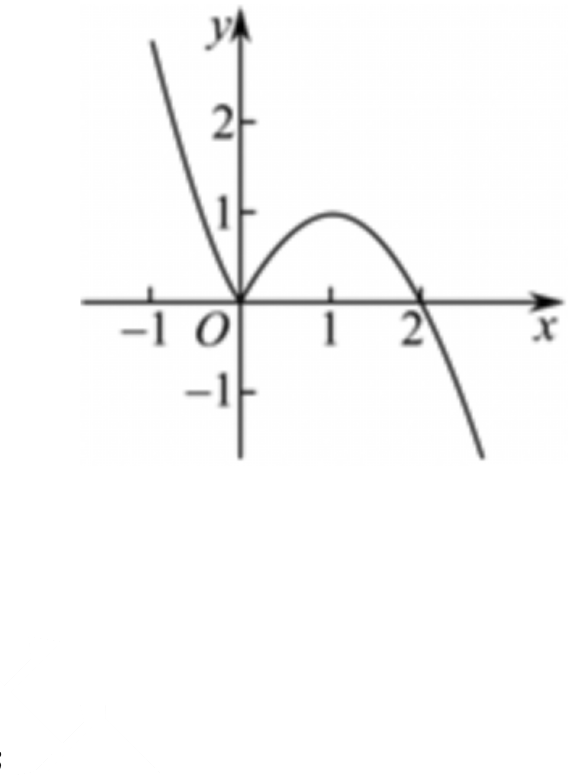
\includegraphics[width=0.20\textwidth]{figures/gao83_q15_graph.png}
\end{center}
\step{由 $[f(x)]^2+af(x)<0$ 得 $[f(x)+a]f(x)<0$，}
\step{当 $a=0$ 时，$[f(x)]^2<0$，不等式无解；}
\step{当 $a>0$ 时，由 $[f(x)+a]f(x)<0$ 得 $-a<f(x)<0$，}
\step{若不等式恰有 $1$ 个整数解，则整数解为 $3$，}
\step{又 $f(3)=-3$，$f(4)=-8$，所以 $-8\leqslant-a<-3$，所以 $3<a\leqslant8$；}
\step{当 $a<0$ 时，由 $[f(x)+a]f(x)<0$ 得 $0<f(x)<-a$，此时有多个解，故舍去；}
\step{综上所述，实数 $a$ 的取值范围为 $(3,8]$. 故选 $C$.}
\solend
\fi

\item 设函数 $f(x)=\begin{cases}\lvert2^x-1\rvert,&x\leqslant2\\ -x+7,&x>2\end{cases}$，若互不相等的实数 $a$、$b$、$c$ 满足 $f(a)=f(b)=f(c)$，
则 $2^a+2^b+2^c$ 的取值范围是\mbox{（\quad）}

\keepwithprev
A. $(8,9)$\qquad B. $(65,129)$\qquad C. $(64,128)$\qquad D. $(66,130)$

\ifanswer
\solbegin
\step{作出函数 $f(x)=\begin{cases}\lvert2^x-1\rvert,&x\leqslant2\\ -x+7,&x>2\end{cases}$ 的图象如图，}
\begin{center}
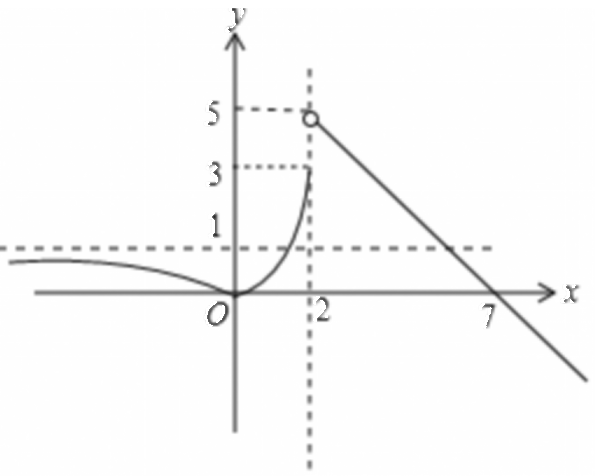
\includegraphics[width=0.22\textwidth]{figures/gao83_q16_graph.png}
\end{center}
\step{不妨设 $a<b<c$，由 $f(a)=f(b)$，得 $1-2^a=2^b-1$，则 $2^a+2^b=2$.}
\step{由 $f(-c)-c+6\in(0,1)$，得 $c\in(6,7)$，则 $64<2^c<128$，}
\step{所以 $66<2^a+2^b+2^c<130$，即 $2^a+2^b+2^c$ 的取值范围是 $(66,130)$. 故选 $D$.}
\solend
\fi

\end{enumerate}

\bigsec{三、解答题}

\begin{enumerate}
\setcounter{enumi}{16}

\item 已知幂函数 $f(x)$ 与一次函数 $g(x)$ 的图象都经过点 $(4,2)$，且 $f(9)=g(5)$.

（1）求 $f(x)$ 与 $g(x)$ 的解析式；

（2）求函数 $h(x)=g(x)-f(x)$ 在 $[0,4]$ 上的值域.

\ansspace*[8]

\ifanswer
\solbegin
\stepm{（1）}{设 $f(x)=x^\alpha$，$g(x)=kx+b$，则 $4^\alpha=2$，即 $\alpha=\dfrac12$，}
\step{$\begin{cases}4k+b=2\\ 3=5k+b\end{cases}$，则 $k=1$，$b=-2$，所以 $f(x)=\sqrt x$，$g(x)=x-2$；}
\stepm{（2）}{$h(x)=g(x)-f(x)=x-\sqrt x-2$，}
\step{令 $t=\sqrt x$，则 $t\in[0,2]$，原函数可化为 $p(t)=t^2-t-2$，}
\step{当 $t=\dfrac12$ 时，函数取得最小值 $-\dfrac94$，当 $t=2$ 时，函数取得最大值 $0$，}
\step{即函数值域为 $\left[-\dfrac94,0\right]$.}
\solend
\fi

\item 目前某县有 $100$ 万人. 经过 $x$ 年后为 $y$ 万人. 如果年平均增长率是 $1.2\%$. 请回答下列问题：

（1）写出 $y$ 关于 $x$ 的函数解析式.

（2）计算 $10$ 年后该县的人口总数（精确到 $0.1$ 万人）.

（3）计算大约多少年后该县的人口总数将达到 $120$ 万（精确到 $1$ 年）.

\ansspace*[9]

\ifanswer
\solbegin
\stepm{（1）}{当 $x=1$ 时，$y=100+100\times1.2\%=100(1+1.2\%)$，}
\step{当 $x=2$ 时，$y=100(1+1.2\%)+100(1+1.2\%)\times1.2\%=100(1+1.2\%)^2$，}
\step{当 $x=3$ 时，$y=100(1+1.2\%)^2+100(1+1.2\%)^2\times1.2\%=100(1+1.2\%)^3$，}
\step{$\cdots\cdots$}
\step{故 $y$ 关于 $x$ 的函数解析式为 $y=100(1+1.2\%)^x\,(x\in\N^*)$；}
\stepm{（2）}{当 $x=10$ 时，$y=100(1+1.2\%)^{10}=100\times1.012^{10}\approx112.7$，}
\step{故 $10$ 年后该县的人口总数约为 $112.7$ 万人；}
\stepm{（3）}{设 $x$ 年后该县的人口总数将达到 $120$ 万，即 $y=100(1+1.2\%)^x=120$，}
\step{解得 $x=\log_{1.012}\dfrac{120}{100}\approx16$，故大约 $16$ 年后该县的人口总数将达到 $120$ 万.}
\solend
\fi

\item 已知 $a>0$ 且 $a\neq1$，$m>0$，函数 $f(x)=(m^2+m-5)a^x$ 是指数函数，且 $f(2)=4$.

（1）求实数 $m$ 和 $a$ 的值；

（2）$f(2x)-2f(x)+2\geqslant nf(x)$ 对任意 $x\in[-1,2]$ 恒成立，求实数 $n$ 的取值范围；

（3）若关于 $x$ 的方程 $f(2x)-(2k+8)f(x)+2k+7b=0$ 有两个不相等的实数根，且一根
大于 $0$，另一根小于 $0$，其中 $k>0$，求整数 $b$ 的最大值.

\ansspace*[11]

\ifanswer
\solbegin
\stepm{（1）}{因为函数 $f(x)=(m^2+m-5)a^x$ 是指数函数，}
\step{所以 $m^2+m-5=1$，即 $m^2+m-6=0$，解得 $m=2$ 或 $m=-3$，}
\step{又 $m>0$，所以 $m=2$，又 $f(2)=a^2=4$，$a>0$ 且 $a\neq1$，所以 $a=2$；}
\stepm{（2）}{由（1）得 $f(x)=2^x$，}
\step{由题意 $2^{2x}-2\cdot2^x+2\geqslant n2^x$ 对任意 $x\in[-1,2]$ 恒成立，}
\step{所以 $n\leqslant2^x-2+\dfrac2{2^x}$ 对任意 $x\in[-1,2]$ 恒成立，则 $n\leqslant\left(2^x-2+\dfrac2{2^x}\right)_{\min}$，}
\step{记 $g(x)=2^x-2+\dfrac2{2^x}$，$x\in[-1,2]$，}
\step{令 $t=2^x$，因为 $x\in[-1,2]$，所以 $t\in\left[\dfrac12,4\right]$，则 $y=t+\dfrac2t-2$，$t\in\left[\dfrac12,4\right]$，}
\step{函数 $y=t+\dfrac2t-2$ 在 $\left[\dfrac12,\sqrt2\right]$ 上严格减，在 $[\sqrt2,4]$ 上严格增，}
\step{所以 $y=t+\dfrac2t-2$ 的最小值为 $\sqrt2+\dfrac2{\sqrt2}-2=2\sqrt2-2$，}
\step{所以 $n\leqslant2\sqrt2-2$，即实数 $n$ 的取值范围为 $(-\infty,2\sqrt2-2]$；}
\stepm{（3）}{方程 $f(2x)-(2k+8)f(x)+2k+7b=0$，}
\step{即方程 $2^{2x}-(2k+8)2^x+2k+7b=0$，即方程 $(2^x)^2-(2k+8)2^x+2k+7b=0$，}
\step{令 $t=2^x>0$，则方程 $t^2-(2k+8)t+2k+7b=0$，}
\step{因为关于 $x$ 的方程 $f(2x)-(2k+8)f(x)+2k+7b=0$ 的一根大于 $0$，另一根小于 $0$，}
\step{所以关于 $t$ 的方程 $t^2-(2k+8)t+2k+7b=0$ 的一根大于 $1$，另一根大于 $0$ 且小于 $1$，}
\step{记 $h(t)=t^2-(2k+8)t+2k+7b$，}
\step{所以 $\begin{cases}h(1)=1^2-(2k+8)\cdot1+2k+7b<0\\ h(0)=2k+7b>0\\ k>0\end{cases}$，所以 $\begin{cases}b<1\\ b>-\dfrac27k\\ k>0\end{cases}$，}
\step{所以整数 $b$ 的最大值为 $0$.}
\solend
\fi

\item 已知幂函数 $f(x)=(p^2-3p+3)x^{p^2-\frac32p-\frac12}$ 满足 $f(2)<f(4)$.

（1）求函数 $f(x)$ 的解析式；

（2）若函数 $g(x)=f^2(x)+mf(x)$，$x\in[1,9]$，是否存在实数 $m$ 使得 $g(x)$ 的最小值为 $0$？
若存在，求出 $m$ 的值；若不存在，说明理由.

（3）若函数 $h(x)=n-f(x+3)$，是否存在实数 $a$、$b\,(a<b)$，使函数 $h(x)$ 在 $[a,b]$ 上的
值域为 $[a,b]$？若存在，求出实数 $n$ 的取值范围；若不存在，说明理由.

\ansspace*[12]

\ifanswer
\solbegin
\stepm{（1）}{因为 $f(x)$ 是幂函数，所以 $p^2-3p+3=1$，解得 $p=1$ 或 $p=2$，}
\step{当 $p=1$ 时，$f(x)=\dfrac1x$，不满足 $f(2)<f(4)$.}
\step{当 $p=2$ 时，$f(x)=\sqrt x$，满足 $f(2)<f(4)$.}
\step{故 $p=2$，函数 $f(x)$ 的解析式为 $f(x)=\sqrt x$；}
\stepm{（2）}{由函数 $g(x)=f^2(x)+mf(x)$，即 $g(x)=(\sqrt x)^2+m\sqrt x$，}
\step{令 $t=\sqrt x$，因为 $x\in[1,9]$，所以 $t\in[1,3]$，}
\step{记 $k(x)=t^2+mt$，其对称轴 $t=-\dfrac m2$，}
\step{①当 $-\dfrac m2\leqslant1$，即 $m\geqslant-2$ 时，则 $k(x)_{\min}=k(1)=1+m=0$，解得 $m=-1$；}
\step{②当 $1<-\dfrac m2<3$ 时，即 $-6<m<-2$，则 $k(x)_{\min}=k\left(-\dfrac m2\right)=-\dfrac{m^2}4=0$，}
\step{解得 $m=0$，不满足，舍去；}
\step{③当 $-\dfrac m2\geqslant3$ 时，即 $m\leqslant-6$ 时，则 $k(x)_{\min}=k(3)=3m+9=0$，解得 $m=-3$，}
\step{不满足，舍去；}
\step{综上所述，存在 $m=-1$ 使得 $g(x)$ 的最小值为 $0$；}
\stepm{（3）}{由函数 $h(x)=n-f(x+3)=n-\sqrt{x+3}$ 在定义域内为严格减函数，}
\step{若存在实数 $a$、$b\,(a<b)$，使函数 $h(x)$ 在 $[a,b]$ 上的值域为 $[a,b]$，}
\step{则 $h(x)=\begin{cases}n-\sqrt{a+3}=b\text{ ①}\\ n-\sqrt{b+3}=a\text{ ②}\end{cases}$，}
\step{两式相减得 $\sqrt{a+3}-\sqrt{b+3}=a-b=(a+3)-(b+3)$，}
\step{所以 $\sqrt{a+3}+\sqrt{b+3}=1$ ③，}
\step{将③代入②得 $n=a+\sqrt{b+3}=a+1-\sqrt{a+3}$，}
\step{令 $t=\sqrt{a+3}$，因为 $a<b$，所以 $0\leqslant t<\dfrac12$，得 $n=t^2-t-2=\left(t-\dfrac12\right)^2-\dfrac94$，}
\step{故实数 $n$ 的取值范围为 $\left(-\dfrac94,-2\right]$.}
\solend
\fi

\item 定理（三角不等式），对于任意的 $a$、$b\in\R$，恒有 $\bigl\lvert\lvert a\rvert-\lvert b\rvert\bigr\rvert\leqslant\lvert a\pm b\rvert\leqslant\lvert a\rvert+\lvert b\rvert$. 定义：
已知 $n\in\N$ 且 $n\geqslant3$，对于有序数组 $a_1$、$a_2$、$\cdots$、$a_n$，称 $\lvert a_1-a_2\rvert+\lvert a_2-a_3\rvert+\cdots+\lvert a_{n-1}-a_n\rvert$
为有序数组 $a_1$、$a_2$、$\cdots$、$a_n$ 的波动距离，记作 $f(a_1,a_2,\cdots,a_n)$，即
$f(a_1,a_2,\cdots,a_n)=\lvert a_1-a_2\rvert+\lvert a_2-a_3\rvert+\cdots+\lvert a_{n-1}-a_n\rvert$，请根据上述信息解决以下几个问题：

（1）求函数 $y=\lvert x-2\rvert+\lvert x-4\rvert$ 的最小值，并指出函数取到最小值时 $x$ 的取值范围；

（2）①求有序数组 $2$、$5$、$3$、$4$ 的波动距离 $f(2,5,3,4)$；

②求证：若 $a$、$b$、$c$、$d\in\R$ 且 $a<b<c$，则 $f(a,b,c,d)\leqslant f(a,c,b,d)$；

（3）同理可证得命题“若 $a$、$b$、$c$、$d\in\R$ 且 $c<b<a$ 时，$f(a,b,c,d)\leqslant f(a,c,b,d)$”也
是真命题（注：该命题无需证明，需要时可直接使用）.

设两两不相等的四个实数 $a_1$、$a_2$、$a_3$、$a_4\in\{3^1,3^2,3^3,3^4\}$，求有序数组 $a_1$、$a_2$、$a_3$、$a_4$ 的
波动距离 $f(a_1,a_2,a_3,a_4)$ 的最大值.

\ansspace*[14]

\ifanswer
\solbegin
\stepm{（1）}{由三角不等式得 $\bigl\lvert\lvert a\rvert-\lvert b\rvert\bigr\rvert\leqslant\lvert a\pm b\rvert\leqslant\lvert a\rvert+\lvert b\rvert$，}
\step{当且仅当 $\lvert a+b\rvert^2=(\lvert a\rvert+\lvert b\rvert)^2$ 时，}
\step{即当 $-ab=\lvert ab\rvert$ 时，即当 $ab\leqslant0$ 时取等号，}
\step{由三角不等式得 $y=\lvert x-2\rvert+\lvert x-4\rvert\geqslant\lvert(x-2)-(x-4)\rvert=2$，}
\step{当且仅当 $(x-2)(x-4)\leqslant0$ 时，即 $2\leqslant x\leqslant4$ 时取等号，}
\step{因此，函数 $y=\lvert x-2\rvert+\lvert x-4\rvert$ 的最小值为 $2$，此时 $x$ 的取值范围是 $[2,4]$.}
\stepm{（2）}{①由题中定义得 $f(2,5,3,4)=\lvert2-5\rvert+\lvert5-3\rvert+\lvert3-4\rvert=6$；}
\step{②$f(a,b,c,d)-f(a,c,b,d)=\lvert a-b\rvert+\lvert c-d\rvert-\lvert a-c\rvert-\lvert b-d\rvert$，}
\step{因为 $a<b<c$，所以 $\lvert a-b\rvert-\lvert a-c\rvert=-\lvert b-c\rvert$，$\lvert c-d\rvert-\lvert b-d\rvert\leqslant\lvert b-c\rvert$，}
\step{所以 $f(a,b,c,d)-f(a,c,b,d)\leqslant0$，即 $f(a,b,c,d)\leqslant f(a,c,b,d)$，}
\stepm{（3）}{$f(a,b,c,d)=\lvert a-b\rvert+\lvert b-c\rvert+\lvert c-d\rvert$}
\step{$=\lvert d-c\rvert+\lvert c-b\rvert+\lvert b-a\rvert=f(d,c,b,a)$，}
\step{当 $f(a_1,a_2,a_3,a_4)$ 取得最大值时，$a_2=\max\{a_1,a_2,a_3\}$ 或 $a_2=\min\{a_1,a_2,a_3\}$，}
\step{同理 $a_3=\max\{a_2,a_3,a_4\}$ 或 $a_3=\min\{a_2,a_3,a_4\}$，}
\step{若 $a_2=\max\{a_1,a_2,a_3\}$，则 $a_2>a_3$，所以 $a_3=\min\{a_2,a_3,a_4\}$，}
\step{故 $f(a_1,a_2,a_3,a_4)=\lvert a_1-a_2\rvert+\lvert a_2-a_3\rvert+\lvert a_3-a_4\rvert=a_2-a_1+a_2-a_3+a_4-a_3$}
\step{$=2a_2+a_4-2a_3-a_1\leqslant2\times3^4+3^3-2\times3^1-3^2=174$，}
\step{当且仅当 $a_1=3^2$，$a_2=3^4$，$a_3=3^1$，$a_4=3^3$ 时取等号，}
\step{所以 $f(3^2,3^4,3^1,3^3)$ 为 $f(a_1,a_2,a_3,a_4)$ 的最大值，}
\step{若 $a_2=\min\{a_1,a_2,a_3\}$，则 $a_2<a_3$，所以 $a_3=\max\{a_2,a_3,a_4\}$，}
\step{同理可得 $f(3^3,3^4,3^1,3^2)$ 为 $f(a_1,a_2,a_3,a_4)$ 的最大值，}
\step{综上所述，$f(a_1,a_2,a_3,a_4)$ 的最大值为 $174$.}
\solend
\fi

\end{enumerate}

\end{document}
"
%
% 原始材料：微信公众号“魔都数学加油站”文章，连载“27学年高一83”；
% 原文标题“27学年高一83——2026-2027年上海市交附闵行高一上周末作业10.23”；
% 原文链接：https://mp.weixin.qq.com/s/t5AfTwQXg4Sj4i_Dl5rgXA。
% 页面标注发布时间 2026-10-26 20:15（上海）。
% 正文为 12 张 PNG 页（`原图/高一83_交附闵行_周末作业10.23/01..12.png`），
% 尺寸混排（第 1—8 页为 4762×6735，第 9—12 页为 2560×3620），均按页序读取。
%
% 篇幅与题号：原卷自第 3 题起编号（第 1、2 题不在原文内）。填空题 3—12（10 题）、
% 选择题 13—16（4 题）、解答题 17—21（5 题），共 19 题。
%
% 讲评版：19 题全部印【解析】，本稿不另提 \ans{}；选择题答案在解析末句“故选 C／B／C／D”。
%
% 副标题：原卷未印副标题。本稿按内容标作“函数与导数”（本卷考幂函数、指数函数、
% 对数与函数应用，属“函数与导数”模块；副标题只用知识模块名，见 README 说明）。
%
% 与原卷的排版差异：
%   ① 原卷每题下直接印【解析】，本稿按全稿惯例将解析置于答案版；
%   ② 原卷未印副标题，本稿补出；填空横线统一排 \blankline[4.4em]；
%   ③ 原卷数集记号排斜体 $R$、$Z$、$N$，本稿按全稿惯例改用 $\R$、$\Z$、$\N$；
%   ④ 第 17—21 题的子问用行内“（1）（2）（3）”段，解析中的子问标号用 \stepm；
%   ⑤ 解答题按惯例加 \ansspace；选择题括号排 \mbox{（\quad）}；
%   ⑥ 第 15、16 题解析各有一幅函数图象，裁自原图（第 6 页）后去粉色水印、转灰度，
%      仅答案版出。
%
% 行数核对：逐题数 \step/\stepm 条数，合计 145 条（Q3：1；Q4：1；Q5：4；Q6：5；
% Q7：2；Q8：7；Q9：10；Q10：5；Q11：6；Q12：8；Q13：3；Q14：4；Q15：8；
% Q16：4；Q17：6；Q18：9；Q19：19；Q20：21；Q21：22）。原卷解析的换行
% 按语意合并，未逐行强拆。
%
\documentclass[a4paper,11pt]{article}
\usepackage{common}

\begin{document}

\examtitlest[4]{2026--2027 年交附闵行高一上周末作业 10.23}{函数与导数}

\bigsec{一、填空题}

\begin{enumerate}
\setcounter{enumi}{2}

\item 已知 $10^a=2$，$10^b=5$，则 $10^{3a-2b}$ 的值为\blankline[4.4em].

\ifanswer
\solbegin
\step{$10^{3a-2b}=\dfrac{10^{3a}}{10^{2b}}=\dfrac{(10^a)^3}{(10^b)^2}=\dfrac{2^3}{5^2}=\dfrac8{25}$.}
\solend
\fi

\item 根式 $a\sqrt{-a}$ 化成分数指数幂是\blankline[4.4em].

\ifanswer
\solbegin
\step{$a\sqrt{-a}=a(-a)^{\frac12}=-(-a)(-a)^{\frac12}=-(-a)^{\frac32}$.}
\solend
\fi

\item 已知数列 $\{a_n\}$ 的通项公式为 $a_n=\left(\dfrac49\right)^{n-1}-\left(\dfrac23\right)^{n-1}$，在下列说法中：①有最大项；
②有最小项；③没有最大项；④没有最小项. 正确的是\blankline[3.6em]（填序号）.

\ifanswer
\solbegin
\step{令 $t=\left(\dfrac23\right)^{n-1}$，则 $t\in\left\{1,\dfrac23,\dfrac49,\dfrac8{27},\cdots\right\}\subset(0,1]$，$t$ 是关于 $n$ 的减函数，}
\step{则 $a_n=t^2-t=\left(t-\dfrac12\right)^2-\dfrac14$，}
\step{所以当 $t=1$ 即 $n=1$ 时 $a_n$ 取得最大为 $0$，当 $t=\dfrac49$ 即 $n=3$ 时 $a_n$ 取得最小为 $-\dfrac{20}{81}$，}
\step{所以 $a_n$ 既有最大项又有最小项，故①和②正确.}
\solend
\fi

\item 已知 $f(x)=\mathrm{e}^{x-\frac12}-\mathrm{e}^{-x+\frac12}+\dfrac{4x}{2x-1}$，则
$f\left(\dfrac1{2020}\right)+f\left(\dfrac2{2020}\right)+f\left(\dfrac3{2020}\right)+\cdots+f\left(\dfrac{1009}{2020}\right)+f\left(\dfrac{1011}{2020}\right)+\cdots+f\left(\dfrac{2019}{2020}\right)$ 的
值为\blankline[4.4em].

\ifanswer
\solbegin
\step{因为 $f(x)+f(1-x)=\mathrm{e}^{x-\frac12}-\mathrm{e}^{-x+\frac12}+\dfrac{4x}{2x-1}+\mathrm{e}^{(1-x)-\frac12}-\mathrm{e}^{-(1-x)+\frac12}+\dfrac{4(1-x)}{2(1-x)-1}$}
\step{$=\dfrac{4x}{2x-1}+\dfrac{4-4x}{1-2x}=\dfrac{4(2x-1)}{2x-1}=4$，}
\step{记 $S=f\left(\dfrac1{2020}\right)+f\left(\dfrac2{2020}\right)+\cdots+f\left(\dfrac{2019}{2020}\right)$，}
\step{又 $S=f\left(\dfrac{2019}{2020}\right)+f\left(\dfrac{2018}{2020}\right)+\cdots+f\left(\dfrac2{2020}\right)+f\left(\dfrac1{2020}\right)$，}
\step{对齐相加得 $2S=2018\times4$，所以 $S=4036$.}
\solend
\fi

\item 不等式 $2^{x^2-2x-3}<\left(\dfrac12\right)^{3(x-1)}$ 的解集为\blankline[4.4em].

\ifanswer
\solbegin
\step{由 $2^{x^2-2x-3}<\left(\dfrac12\right)^{3(x-1)}$ 得 $x^2-2x-3<-3(x-1)$，即 $x^2+x-6<0$，}
\step{故解集为 $(-3,2)$.}
\solend
\fi

\item 函数 $f(x)=x^{\ln5}+x^{\ln12}-13^{\ln x}$ 的零点是\blankline[4.4em]. 附：$a^{\log_bc}=c^{\log_ba}$
（$a>0$，$b>0$，$c>0$，$b\neq1$）.

\ifanswer
\solbegin
\step{函数 $f(x)=x^{\ln5}+x^{\ln12}-13^{\ln x}$，}
\step{若 $f(x)=x^{\ln5}+x^{\ln12}-13^{\ln x}=0$，变形得 $x^{\ln5}+x^{\ln12}=13^{\ln x}$，}
\step{又 $a^{\log_bc}=c^{\log_ba}$（$a>0$，$b>0$，$c>0$，$b\neq1$），得 $5^{\ln x}+12^{\ln x}=13^{\ln x}$，}
\step{令 $g(t)=\left(\dfrac5{13}\right)^t+\left(\dfrac{12}{13}\right)^t-1$，易得 $g(t)$ 严格减，所以 $g(t)=0$ 至多有一解，}
\step{即 $\left(\dfrac5{13}\right)^t+\left(\dfrac{12}{13}\right)^t-1=0$ 至多有一解，变形得方程 $5^t+12^t=13^t$ 至多有一解，}
\step{易得 $t=2$ 时，有 $5^2+12^2=13^2$ 成立，则方程 $5^t+12^t=13^t$ 有唯一解 $t=2$，}
\step{即 $\ln x=2$，解得 $x=\mathrm{e}^2$，即函数 $f(x)$ 的零点为 $\mathrm{e}^2$.}
\solend
\fi

\item 已知幂函数 $f(x)=(m^2-2m-2)x^{m^2+m-2}$ 在 $(0,+\infty)$ 上是严格减函数，则不等式
$f(x-1)<f(3-2x)$ 的解集为\blankline[4.4em].

\ifanswer
\solbegin
\step{因为 $f(x)$ 为幂函数，所以 $m^2-2m-2=1$，解得 $m=-1$ 或 $m=3$；}
\step{当 $m=3$ 时，$f(x)=x^{10}$ 在 $(0,+\infty)$ 上严格增，不合题意；}
\step{当 $m=-1$ 时，$f(x)=x^{-2}$ 在 $(0,+\infty)$ 上严格减，符合题意；}
\step{综上所述，$m=-1$；}
\step{因为 $f(x)=x^{-2}$ 的定义域为 $(-\infty,0)\cup(0,+\infty)$，$f(-x)=(-x)^{-2}=x^{-2}=f(x)$，}
\step{所以 $f(x)$ 为定义在 $(-\infty,0)\cup(0,+\infty)$ 上的偶函数，}
\step{故 $f(x-1)=f(\lvert x-1\rvert)$，$f(3-2x)=f(\lvert3-2x\rvert)$，}
\step{$f(x-1)<f(3-2x)\Rightarrow f(\lvert x-1\rvert)<f(\lvert3-2x\rvert)\Rightarrow\lvert x-1\rvert>\lvert3-2x\rvert$}
\step{且 $\lvert x-1\rvert\neq0$，$\lvert3-2x\rvert\neq0$，解得 $\dfrac43<x<\dfrac32$ 或 $\dfrac32<x<2$，}
\step{所以 $f(x-1)<f(3-2x)$ 的解集为 $\left(\dfrac43,\dfrac32\right)\cup\left(\dfrac32,2\right)$.}
\solend
\fi

\item 若实数 $x_1$、$x_2$ 满足 $\mathrm{e}^{x_1}+x_1-3=0$，$x_2\ln x_2+3x_2-1=0$，则 $\dfrac{x_1x_2+1}{x_2}$ 的值为\blankline[4.4em].

\ifanswer
\solbegin
\step{易得 $x_2>0$，则 $\ln x_2+3-\dfrac1{x_2}=0$，即 $\mathrm{e}^{-\ln x_2}+(-\ln x_2)-3=0$.}
\step{设 $f(x)=\mathrm{e}^x+x-3$，则函数 $f(x)$ 在 $(-\infty,+\infty)$ 上严格增.}
\step{由 $\mathrm{e}^{x_1}+x_1-3=0$，$\mathrm{e}^{-\ln x_2}+(-\ln x_2)-3=0$，得 $f(x_1)=0$，$f(-\ln x_2)=0$，}
\step{所以 $f(x_1)=f(-\ln x_2)$，得 $x_1=-\ln x_2$，即 $\ln x_2=-x_1$，所以 $x_2=\mathrm{e}^{-x_1}$，得 $\dfrac1{x_2}=\mathrm{e}^{x_1}$.}
\step{因为 $\mathrm{e}^{x_1}+x_1-3=0$，所以 $\mathrm{e}^{x_1}+x_1=3$，所以 $\dfrac{x_1x_2+1}{x_2}=x_1+\dfrac1{x_2}=\mathrm{e}^{x_1}+x_1=3$.}
\solend
\fi

\item 已知 $\alpha$、$\beta$ 是方程 $9^x-2m\cdot3^x+m^2-1=0$ 的两个根，若 $\alpha+\beta=1$，则 $\alpha\beta=\blankline[4.4em]$.

\ifanswer
\solbegin
\step{由题意得方程 $9^x-2m\cdot3^x+m^2-1=0$ 有两个根，}
\step{则方程 $t^2-2mt+m^2-1=0$ 有二正根，则 $\begin{cases}\Delta=4m^2-4(m^2-1)\geqslant0\\ 2m>0\\ m^2-1>0\end{cases}$，解得 $m>1$，}
\step{又 $\alpha$、$\beta$ 是方程 $9^x-2m\cdot3^x+m^2-1=0$ 的两个根，则 $3^\alpha\times3^\beta=m^2-1$，}
\step{又 $\alpha+\beta=1$，则 $m^2-1=3^{\alpha+\beta}=3$，解得 $m=2$ 或 $m=-2$（舍），}
\step{则 $3^\alpha+3^\beta=2m=4$，又 $\alpha=1-\beta$，则 $3^{1-\beta}+3^\beta=4$，解得 $\beta=0$ 或 $\beta=1$，}
\step{则 $\begin{cases}\alpha=1\\ \beta=0\end{cases}$ 或 $\begin{cases}\alpha=0\\ \beta=1\end{cases}$，则 $\alpha\beta=0$.}
\solend
\fi

\item 已知实数 $a,b,c\in(1,+\infty)$，满足 $a^{\log_ba}\cdot b^{\log_cb}\cdot c^{\log_ac}=100$，则 $abc$ 的最大值为\blankline[4.4em].

\ifanswer
\solbegin
\step{由换底公式得 $\log_ba=\dfrac{\ln a}{\ln b}$，$\log_cb=\dfrac{\ln b}{\ln c}$，$\log_ac=\dfrac{\ln c}{\ln a}$，}
\step{设 $X=\ln a$，$Y=\ln b$，$Z=\ln c$，得 $a=\mathrm{e}^X$，$b=\mathrm{e}^Y$，$c=\mathrm{e}^Z$，}
\step{代入得 $a^{\log_ba}\cdot b^{\log_cb}\cdot c^{\log_ac}=a^{\frac{\ln a}{\ln b}}\cdot b^{\frac{\ln b}{\ln c}}\cdot c^{\frac{\ln c}{\ln a}}=(\mathrm{e}^X)^{\frac XY}\cdot(\mathrm{e}^Y)^{\frac YZ}\cdot(\mathrm{e}^Z)^{\frac ZX}=100$，}
\step{即 $\mathrm{e}^{\frac{X^2}Y+\frac{Y^2}Z+\frac{Z^2}X}=100$，两边取对数得 $\dfrac{X^2}Y+\dfrac{Y^2}Z+\dfrac{Z^2}X=\ln100$.}
\step{由 $a,b,c\in(1,+\infty)$，得 $X>0$，$Y>0$，$Z>0$，}
\step{由柯西不等式，得 $\left(\dfrac{X^2}Y+\dfrac{Y^2}Z+\dfrac{Z^2}X\right)(X+Y+Z)\geqslant(X+Y+Z)^2$，}
\step{即 $X+Y+Z\leqslant\dfrac{X^2}Y+\dfrac{Y^2}Z+\dfrac{Z^2}X=\ln100$，当且仅当 $X=Y=Z$ 时取等号，}
\step{因此 $(X+Y+Z)_{\max}=\ln100$，所以 $(abc)_{\max}=\mathrm{e}^{(X+Y+Z)_{\max}}=\mathrm{e}^{\ln100}=100$.}
\solend
\fi

\end{enumerate}

\bigsec{二、选择题}

\begin{enumerate}
\setcounter{enumi}{12}

\item 已知集合 $A=\{x\mid x=2k,k\in\Z\}$，$B=\{x\mid x=4k+2,\,k\in\Z\}$，则 $A\cup B=\mbox{（\quad）}$

\keepwithprev
A. $B$\qquad B. $\R$\qquad C. $A$\qquad D. 以上都不是

\ifanswer
\solbegin
\step{$B=\{x\mid x=4k+2,k\in\Z\}=\{x\mid x=2(2k+1),k\in\Z\}$，它表示奇数的 $2$ 倍组成的集合，}
\step{$A=\{x\mid x=2k,k\in\Z\}$，即集合 $A$ 是整数的 $2$ 倍组成的集合，}
\step{则 $B\subseteq A$，则 $A\cup B=A$. 故选 $C$.}
\solend
\fi

\item 教室通风的目的是通过空气的流动，排出室内的污浊空气和致病微生物，降低室内二氧化碳和致病微生物的浓度，送进室外的新鲜空气. 按照国家标准，教室内空气中二氧化碳日平均最高容许浓度应小于等于 $0.1\%$. 经测定，刚下课时，空气中含有 $0.2\%$ 的二氧化碳，若开窗通风后教室内二氧化碳的浓度为 $y\%$，且 $y$ 随时间 $t$（单位：分钟）的变化规律可以用函数 $y=0.05+\lambda\mathrm{e}^{-\frac t{12}}\,(\lambda\in\R)$ 描述，则该教室内的二氧化碳浓度达到国家标准至少需要的时间为\mbox{（\quad）}

\keepwithprev
A. $10$ 分钟\qquad B. $14$ 分钟\qquad C. $15$ 分钟\qquad D. $20$ 分钟

\ifanswer
\solbegin
\step{由题意得，当 $t=0$ 时，$y=0.2$，即 $0.05+\lambda\mathrm{e}^0=0.2$，解得 $\lambda=0.15$，}
\step{所以 $y=0.05+0.15\mathrm{e}^{-\frac t{12}}$，由题意得 $0.05+0.15\mathrm{e}^{-\frac t{12}}\leqslant0.1$，即 $\mathrm{e}^{-\frac t{12}}\leqslant\dfrac13$，}
\step{两边取对数得 $-\dfrac t{12}\leqslant-\ln3$，所以 $t\geqslant12\ln3\approx13.2$，}
\step{所以该教室内的二氧化碳浓度达到国家标准至少需要的时间为 $14$ 分钟. 故选 $B$.}
\solend
\fi

\item 已知函数 $f(x)=\begin{cases}-x^2+2x,&x\geqslant0\\ x^2-2x,&x<0\end{cases}$，若关于 $x$ 的不等式 $[f(x)]^2+af(x)<0$ 恰有 $1$ 个整数
解，则实数 $a$ 的最大值为\mbox{（\quad）}

\keepwithprev
A. $-2$\qquad B. $3$\qquad C. $8$\qquad D. $9$

\ifanswer
\solbegin
\step{作出 $f(x)$ 的图象，如图所示：}
\begin{center}
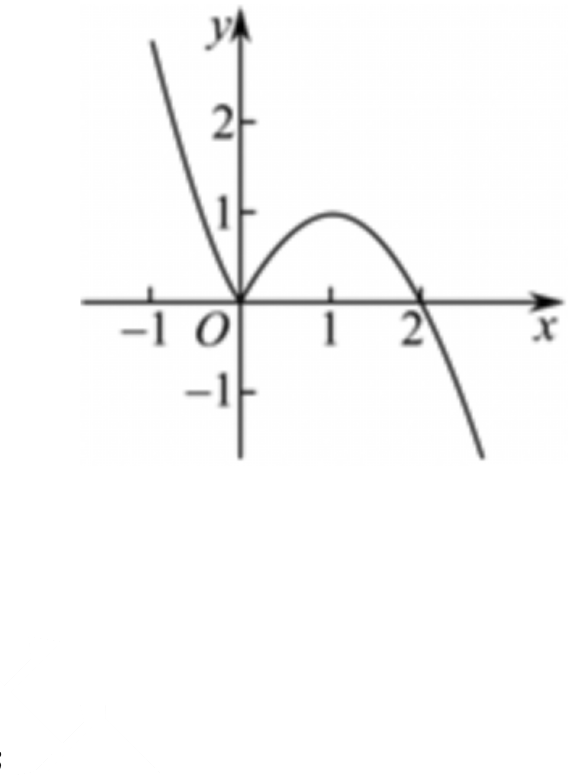
\includegraphics[width=0.20\textwidth]{figures/gao83_q15_graph.png}
\end{center}
\step{由 $[f(x)]^2+af(x)<0$ 得 $[f(x)+a]f(x)<0$，}
\step{当 $a=0$ 时，$[f(x)]^2<0$，不等式无解；}
\step{当 $a>0$ 时，由 $[f(x)+a]f(x)<0$ 得 $-a<f(x)<0$，}
\step{若不等式恰有 $1$ 个整数解，则整数解为 $3$，}
\step{又 $f(3)=-3$，$f(4)=-8$，所以 $-8\leqslant-a<-3$，所以 $3<a\leqslant8$；}
\step{当 $a<0$ 时，由 $[f(x)+a]f(x)<0$ 得 $0<f(x)<-a$，此时有多个解，故舍去；}
\step{综上所述，实数 $a$ 的取值范围为 $(3,8]$. 故选 $C$.}
\solend
\fi

\item 设函数 $f(x)=\begin{cases}\lvert2^x-1\rvert,&x\leqslant2\\ -x+7,&x>2\end{cases}$，若互不相等的实数 $a$、$b$、$c$ 满足 $f(a)=f(b)=f(c)$，
则 $2^a+2^b+2^c$ 的取值范围是\mbox{（\quad）}

\keepwithprev
A. $(8,9)$\qquad B. $(65,129)$\qquad C. $(64,128)$\qquad D. $(66,130)$

\ifanswer
\solbegin
\step{作出函数 $f(x)=\begin{cases}\lvert2^x-1\rvert,&x\leqslant2\\ -x+7,&x>2\end{cases}$ 的图象如图，}
\begin{center}
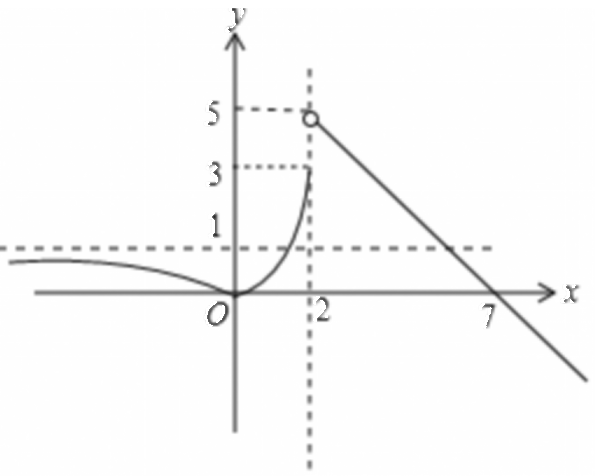
\includegraphics[width=0.22\textwidth]{figures/gao83_q16_graph.png}
\end{center}
\step{不妨设 $a<b<c$，由 $f(a)=f(b)$，得 $1-2^a=2^b-1$，则 $2^a+2^b=2$.}
\step{由 $f(-c)-c+6\in(0,1)$，得 $c\in(6,7)$，则 $64<2^c<128$，}
\step{所以 $66<2^a+2^b+2^c<130$，即 $2^a+2^b+2^c$ 的取值范围是 $(66,130)$. 故选 $D$.}
\solend
\fi

\end{enumerate}

\bigsec{三、解答题}

\begin{enumerate}
\setcounter{enumi}{16}

\item 已知幂函数 $f(x)$ 与一次函数 $g(x)$ 的图象都经过点 $(4,2)$，且 $f(9)=g(5)$.

（1）求 $f(x)$ 与 $g(x)$ 的解析式；

（2）求函数 $h(x)=g(x)-f(x)$ 在 $[0,4]$ 上的值域.

\ansspace*[8]

\ifanswer
\solbegin
\stepm{（1）}{设 $f(x)=x^\alpha$，$g(x)=kx+b$，则 $4^\alpha=2$，即 $\alpha=\dfrac12$，}
\step{$\begin{cases}4k+b=2\\ 3=5k+b\end{cases}$，则 $k=1$，$b=-2$，所以 $f(x)=\sqrt x$，$g(x)=x-2$；}
\stepm{（2）}{$h(x)=g(x)-f(x)=x-\sqrt x-2$，}
\step{令 $t=\sqrt x$，则 $t\in[0,2]$，原函数可化为 $p(t)=t^2-t-2$，}
\step{当 $t=\dfrac12$ 时，函数取得最小值 $-\dfrac94$，当 $t=2$ 时，函数取得最大值 $0$，}
\step{即函数值域为 $\left[-\dfrac94,0\right]$.}
\solend
\fi

\item 目前某县有 $100$ 万人. 经过 $x$ 年后为 $y$ 万人. 如果年平均增长率是 $1.2\%$. 请回答下列问题：

（1）写出 $y$ 关于 $x$ 的函数解析式.

（2）计算 $10$ 年后该县的人口总数（精确到 $0.1$ 万人）.

（3）计算大约多少年后该县的人口总数将达到 $120$ 万（精确到 $1$ 年）.

\ansspace*[9]

\ifanswer
\solbegin
\stepm{（1）}{当 $x=1$ 时，$y=100+100\times1.2\%=100(1+1.2\%)$，}
\step{当 $x=2$ 时，$y=100(1+1.2\%)+100(1+1.2\%)\times1.2\%=100(1+1.2\%)^2$，}
\step{当 $x=3$ 时，$y=100(1+1.2\%)^2+100(1+1.2\%)^2\times1.2\%=100(1+1.2\%)^3$，}
\step{$\cdots\cdots$}
\step{故 $y$ 关于 $x$ 的函数解析式为 $y=100(1+1.2\%)^x\,(x\in\N^*)$；}
\stepm{（2）}{当 $x=10$ 时，$y=100(1+1.2\%)^{10}=100\times1.012^{10}\approx112.7$，}
\step{故 $10$ 年后该县的人口总数约为 $112.7$ 万人；}
\stepm{（3）}{设 $x$ 年后该县的人口总数将达到 $120$ 万，即 $y=100(1+1.2\%)^x=120$，}
\step{解得 $x=\log_{1.012}\dfrac{120}{100}\approx16$，故大约 $16$ 年后该县的人口总数将达到 $120$ 万.}
\solend
\fi

\item 已知 $a>0$ 且 $a\neq1$，$m>0$，函数 $f(x)=(m^2+m-5)a^x$ 是指数函数，且 $f(2)=4$.

（1）求实数 $m$ 和 $a$ 的值；

（2）$f(2x)-2f(x)+2\geqslant nf(x)$ 对任意 $x\in[-1,2]$ 恒成立，求实数 $n$ 的取值范围；

（3）若关于 $x$ 的方程 $f(2x)-(2k+8)f(x)+2k+7b=0$ 有两个不相等的实数根，且一根
大于 $0$，另一根小于 $0$，其中 $k>0$，求整数 $b$ 的最大值.

\ansspace*[11]

\ifanswer
\solbegin
\stepm{（1）}{因为函数 $f(x)=(m^2+m-5)a^x$ 是指数函数，}
\step{所以 $m^2+m-5=1$，即 $m^2+m-6=0$，解得 $m=2$ 或 $m=-3$，}
\step{又 $m>0$，所以 $m=2$，又 $f(2)=a^2=4$，$a>0$ 且 $a\neq1$，所以 $a=2$；}
\stepm{（2）}{由（1）得 $f(x)=2^x$，}
\step{由题意 $2^{2x}-2\cdot2^x+2\geqslant n2^x$ 对任意 $x\in[-1,2]$ 恒成立，}
\step{所以 $n\leqslant2^x-2+\dfrac2{2^x}$ 对任意 $x\in[-1,2]$ 恒成立，则 $n\leqslant\left(2^x-2+\dfrac2{2^x}\right)_{\min}$，}
\step{记 $g(x)=2^x-2+\dfrac2{2^x}$，$x\in[-1,2]$，}
\step{令 $t=2^x$，因为 $x\in[-1,2]$，所以 $t\in\left[\dfrac12,4\right]$，则 $y=t+\dfrac2t-2$，$t\in\left[\dfrac12,4\right]$，}
\step{函数 $y=t+\dfrac2t-2$ 在 $\left[\dfrac12,\sqrt2\right]$ 上严格减，在 $[\sqrt2,4]$ 上严格增，}
\step{所以 $y=t+\dfrac2t-2$ 的最小值为 $\sqrt2+\dfrac2{\sqrt2}-2=2\sqrt2-2$，}
\step{所以 $n\leqslant2\sqrt2-2$，即实数 $n$ 的取值范围为 $(-\infty,2\sqrt2-2]$；}
\stepm{（3）}{方程 $f(2x)-(2k+8)f(x)+2k+7b=0$，}
\step{即方程 $2^{2x}-(2k+8)2^x+2k+7b=0$，即方程 $(2^x)^2-(2k+8)2^x+2k+7b=0$，}
\step{令 $t=2^x>0$，则方程 $t^2-(2k+8)t+2k+7b=0$，}
\step{因为关于 $x$ 的方程 $f(2x)-(2k+8)f(x)+2k+7b=0$ 的一根大于 $0$，另一根小于 $0$，}
\step{所以关于 $t$ 的方程 $t^2-(2k+8)t+2k+7b=0$ 的一根大于 $1$，另一根大于 $0$ 且小于 $1$，}
\step{记 $h(t)=t^2-(2k+8)t+2k+7b$，}
\step{所以 $\begin{cases}h(1)=1^2-(2k+8)\cdot1+2k+7b<0\\ h(0)=2k+7b>0\\ k>0\end{cases}$，所以 $\begin{cases}b<1\\ b>-\dfrac27k\\ k>0\end{cases}$，}
\step{所以整数 $b$ 的最大值为 $0$.}
\solend
\fi

\item 已知幂函数 $f(x)=(p^2-3p+3)x^{p^2-\frac32p-\frac12}$ 满足 $f(2)<f(4)$.

（1）求函数 $f(x)$ 的解析式；

（2）若函数 $g(x)=f^2(x)+mf(x)$，$x\in[1,9]$，是否存在实数 $m$ 使得 $g(x)$ 的最小值为 $0$？
若存在，求出 $m$ 的值；若不存在，说明理由.

（3）若函数 $h(x)=n-f(x+3)$，是否存在实数 $a$、$b\,(a<b)$，使函数 $h(x)$ 在 $[a,b]$ 上的
值域为 $[a,b]$？若存在，求出实数 $n$ 的取值范围；若不存在，说明理由.

\ansspace*[12]

\ifanswer
\solbegin
\stepm{（1）}{因为 $f(x)$ 是幂函数，所以 $p^2-3p+3=1$，解得 $p=1$ 或 $p=2$，}
\step{当 $p=1$ 时，$f(x)=\dfrac1x$，不满足 $f(2)<f(4)$.}
\step{当 $p=2$ 时，$f(x)=\sqrt x$，满足 $f(2)<f(4)$.}
\step{故 $p=2$，函数 $f(x)$ 的解析式为 $f(x)=\sqrt x$；}
\stepm{（2）}{由函数 $g(x)=f^2(x)+mf(x)$，即 $g(x)=(\sqrt x)^2+m\sqrt x$，}
\step{令 $t=\sqrt x$，因为 $x\in[1,9]$，所以 $t\in[1,3]$，}
\step{记 $k(x)=t^2+mt$，其对称轴 $t=-\dfrac m2$，}
\step{①当 $-\dfrac m2\leqslant1$，即 $m\geqslant-2$ 时，则 $k(x)_{\min}=k(1)=1+m=0$，解得 $m=-1$；}
\step{②当 $1<-\dfrac m2<3$ 时，即 $-6<m<-2$，则 $k(x)_{\min}=k\left(-\dfrac m2\right)=-\dfrac{m^2}4=0$，}
\step{解得 $m=0$，不满足，舍去；}
\step{③当 $-\dfrac m2\geqslant3$ 时，即 $m\leqslant-6$ 时，则 $k(x)_{\min}=k(3)=3m+9=0$，解得 $m=-3$，}
\step{不满足，舍去；}
\step{综上所述，存在 $m=-1$ 使得 $g(x)$ 的最小值为 $0$；}
\stepm{（3）}{由函数 $h(x)=n-f(x+3)=n-\sqrt{x+3}$ 在定义域内为严格减函数，}
\step{若存在实数 $a$、$b\,(a<b)$，使函数 $h(x)$ 在 $[a,b]$ 上的值域为 $[a,b]$，}
\step{则 $h(x)=\begin{cases}n-\sqrt{a+3}=b\text{ ①}\\ n-\sqrt{b+3}=a\text{ ②}\end{cases}$，}
\step{两式相减得 $\sqrt{a+3}-\sqrt{b+3}=a-b=(a+3)-(b+3)$，}
\step{所以 $\sqrt{a+3}+\sqrt{b+3}=1$ ③，}
\step{将③代入②得 $n=a+\sqrt{b+3}=a+1-\sqrt{a+3}$，}
\step{令 $t=\sqrt{a+3}$，因为 $a<b$，所以 $0\leqslant t<\dfrac12$，得 $n=t^2-t-2=\left(t-\dfrac12\right)^2-\dfrac94$，}
\step{故实数 $n$ 的取值范围为 $\left(-\dfrac94,-2\right]$.}
\solend
\fi

\item 定理（三角不等式），对于任意的 $a$、$b\in\R$，恒有 $\bigl\lvert\lvert a\rvert-\lvert b\rvert\bigr\rvert\leqslant\lvert a\pm b\rvert\leqslant\lvert a\rvert+\lvert b\rvert$. 定义：
已知 $n\in\N$ 且 $n\geqslant3$，对于有序数组 $a_1$、$a_2$、$\cdots$、$a_n$，称 $\lvert a_1-a_2\rvert+\lvert a_2-a_3\rvert+\cdots+\lvert a_{n-1}-a_n\rvert$
为有序数组 $a_1$、$a_2$、$\cdots$、$a_n$ 的波动距离，记作 $f(a_1,a_2,\cdots,a_n)$，即
$f(a_1,a_2,\cdots,a_n)=\lvert a_1-a_2\rvert+\lvert a_2-a_3\rvert+\cdots+\lvert a_{n-1}-a_n\rvert$，请根据上述信息解决以下几个问题：

（1）求函数 $y=\lvert x-2\rvert+\lvert x-4\rvert$ 的最小值，并指出函数取到最小值时 $x$ 的取值范围；

（2）①求有序数组 $2$、$5$、$3$、$4$ 的波动距离 $f(2,5,3,4)$；

②求证：若 $a$、$b$、$c$、$d\in\R$ 且 $a<b<c$，则 $f(a,b,c,d)\leqslant f(a,c,b,d)$；

（3）同理可证得命题“若 $a$、$b$、$c$、$d\in\R$ 且 $c<b<a$ 时，$f(a,b,c,d)\leqslant f(a,c,b,d)$”也
是真命题（注：该命题无需证明，需要时可直接使用）.

设两两不相等的四个实数 $a_1$、$a_2$、$a_3$、$a_4\in\{3^1,3^2,3^3,3^4\}$，求有序数组 $a_1$、$a_2$、$a_3$、$a_4$ 的
波动距离 $f(a_1,a_2,a_3,a_4)$ 的最大值.

\ansspace*[14]

\ifanswer
\solbegin
\stepm{（1）}{由三角不等式得 $\bigl\lvert\lvert a\rvert-\lvert b\rvert\bigr\rvert\leqslant\lvert a\pm b\rvert\leqslant\lvert a\rvert+\lvert b\rvert$，}
\step{当且仅当 $\lvert a+b\rvert^2=(\lvert a\rvert+\lvert b\rvert)^2$ 时，}
\step{即当 $-ab=\lvert ab\rvert$ 时，即当 $ab\leqslant0$ 时取等号，}
\step{由三角不等式得 $y=\lvert x-2\rvert+\lvert x-4\rvert\geqslant\lvert(x-2)-(x-4)\rvert=2$，}
\step{当且仅当 $(x-2)(x-4)\leqslant0$ 时，即 $2\leqslant x\leqslant4$ 时取等号，}
\step{因此，函数 $y=\lvert x-2\rvert+\lvert x-4\rvert$ 的最小值为 $2$，此时 $x$ 的取值范围是 $[2,4]$.}
\stepm{（2）}{①由题中定义得 $f(2,5,3,4)=\lvert2-5\rvert+\lvert5-3\rvert+\lvert3-4\rvert=6$；}
\step{②$f(a,b,c,d)-f(a,c,b,d)=\lvert a-b\rvert+\lvert c-d\rvert-\lvert a-c\rvert-\lvert b-d\rvert$，}
\step{因为 $a<b<c$，所以 $\lvert a-b\rvert-\lvert a-c\rvert=-\lvert b-c\rvert$，$\lvert c-d\rvert-\lvert b-d\rvert\leqslant\lvert b-c\rvert$，}
\step{所以 $f(a,b,c,d)-f(a,c,b,d)\leqslant0$，即 $f(a,b,c,d)\leqslant f(a,c,b,d)$，}
\stepm{（3）}{$f(a,b,c,d)=\lvert a-b\rvert+\lvert b-c\rvert+\lvert c-d\rvert$}
\step{$=\lvert d-c\rvert+\lvert c-b\rvert+\lvert b-a\rvert=f(d,c,b,a)$，}
\step{当 $f(a_1,a_2,a_3,a_4)$ 取得最大值时，$a_2=\max\{a_1,a_2,a_3\}$ 或 $a_2=\min\{a_1,a_2,a_3\}$，}
\step{同理 $a_3=\max\{a_2,a_3,a_4\}$ 或 $a_3=\min\{a_2,a_3,a_4\}$，}
\step{若 $a_2=\max\{a_1,a_2,a_3\}$，则 $a_2>a_3$，所以 $a_3=\min\{a_2,a_3,a_4\}$，}
\step{故 $f(a_1,a_2,a_3,a_4)=\lvert a_1-a_2\rvert+\lvert a_2-a_3\rvert+\lvert a_3-a_4\rvert=a_2-a_1+a_2-a_3+a_4-a_3$}
\step{$=2a_2+a_4-2a_3-a_1\leqslant2\times3^4+3^3-2\times3^1-3^2=174$，}
\step{当且仅当 $a_1=3^2$，$a_2=3^4$，$a_3=3^1$，$a_4=3^3$ 时取等号，}
\step{所以 $f(3^2,3^4,3^1,3^3)$ 为 $f(a_1,a_2,a_3,a_4)$ 的最大值，}
\step{若 $a_2=\min\{a_1,a_2,a_3\}$，则 $a_2<a_3$，所以 $a_3=\max\{a_2,a_3,a_4\}$，}
\step{同理可得 $f(3^3,3^4,3^1,3^2)$ 为 $f(a_1,a_2,a_3,a_4)$ 的最大值，}
\step{综上所述，$f(a_1,a_2,a_3,a_4)$ 的最大值为 $174$.}
\solend
\fi

\end{enumerate}

\end{document}
